\documentclass[a4paper, 11pt, openright]{book} % book template, paper size is b5

%%%%%%%%%%%%%%%%%%%%%%%%%%%%%%%%%%%%%%%%%%%%%%%%%%%%%%%%%%%%%%%%%%%%%%%%%%%%%%%%
% PACKAGES %%%%%%%%%%%%%%%%%%%%%%%%%%%%%%%%%%%%%%%%%%%%%%%%%%%%%%%%%%%%%%%%%%%%%
%%%%%%%%%%%%%%%%%%%%%%%%%%%%%%%%%%%%%%%%%%%%%%%%%%%%%%%%%%%%%%%%%%%%%%%%%%%%%%%%

% Suppress some warnings -------------------------------------------------------
\usepackage{silence}
\WarningsOff[everypage] % Suppress warnings related to package everypage
%\pdfsuppresswarningpagegroup=1

\setlength{\parskip}{0pt}        % no space between paragraphs

% Maths ------------------------------------------------------------------------
\usepackage{amsmath}             % principal package for serious mathematical typesetting
\usepackage{empheq}              % emphasize equations
\usepackage{mathtools}           % improved version of amsmath
\usepackage{amssymb}             % particular mathematical symbols
\usepackage{bm}                  % bold math formula, similar to '\mathbf'
\usepackage{mathrsfs}            % math upper case letter fonts
\usepackage{amsthm}              % to define theorems, lemmas, etc
\usepackage{thmtools}            % to define theorems, lemmas, etc

\declaretheoremstyle[
  headfont=\normalfont\bfseries,
  notefont=\normalfont\bfseries\itshape,
  bodyfont=\itshape,
  numbered=unless unique,
  spaceabove=1.0em plus 0.25em minus 0.25em,
  qed={$\blacksquare$}, %\qedsymbol
  spacebelow=1.0em plus 0.25em minus 0.25em,
]{defstyle}

\declaretheorem[
  style=defstyle,
  title=Definition,
  refname={definition},
  Refname={Definition}
]{definition}

\declaretheoremstyle[
  headfont=\normalfont\bfseries,
  notefont=\normalfont\bfseries\itshape,
  bodyfont=\normalfont,
  numbered=unless unique,
  spaceabove=1.0em plus 0.25em minus 0.25em,
  qed={$\blacksquare$}, %\qedsymbol
  spacebelow=1.0em plus 0.25em minus 0.25em,
]{exstyle}

\declaretheorem[
  style=exstyle,
  title=Example,
  refname={example},
  Refname={Example}
]{example}

\renewenvironment{bmatrix}%
  {\left[\hspace{-.75\arraycolsep}\array{*{\value{MaxMatrixCols}}{c}}}%
  {\endarray\hspace{-.75\arraycolsep}\right]}

\newenvironment{system}%
  {\left\{\begin{array}{@{}r@{~}c@{~}l}}%
    {\end{array}\hspace{-.75\arraycolsep}\right.}

\renewenvironment{cases}%
  {\left\{\begin{array}{@{}l@{\;}lr@{}}}%
  {\end{array}\hspace{-.75\arraycolsep}\right.}

% Document settings ------------------------------------------------------------
\usepackage{geometry}            % change margins of the document
\usepackage{acronym}             % to define abbreviations
\usepackage{rotating}            % rotate objects

% Text settings ----------------------------------------------------------------
\usepackage[dvipsnames]{xcolor}  % color the text
\usepackage{soul}                % to strike-through text
\usepackage{tcolorbox}           % create a colored box wrapping the text
\usepackage[final]{microtype}    % improves the spacing between words and letters
\usepackage{appendix}       % to create appendices
\usepackage[english]{babel}      % useful to interpret the language of the document
\usepackage[T1]{fontenc}         % to write correctly in Italian
\usepackage[utf8]{inputenc}      % to correctly write accented letter and other symbols
%\usepackage[latin1]{inputenc}    % codec input useful to write docs in Italian
%\usepackage[normalem]{ulem}      % underline command which will break over line ends
\usepackage{listings}            % to include code in the document
\usepackage{realboxes}           % to create boxes around text
\usepackage{url}                 % to write url in the document

\urlstyle{tt}                    % teletype font of the document (forced in the bibliography)
\lstset{                         % settings for the listings package
  basicstyle=\ttfamily,
  columns=fullflexible,
  keepspaces=false
}

\lstnewenvironment{mapleinline}[1][]
  {\lstset{
    frame=none,
    linewidth=1.0\textwidth,
    aboveskip=0.25em,
    belowskip=0.25em,
    #1
  }}{}

\lstnewenvironment{mapleboxed}[1][]
  {\lstset{
    frame=tbrl,
    linewidth=1.0\textwidth,
    belowskip=-0.5em,
    #1
  }}{}

% Fonts ------------------------------------------------------------------------
%\usepackage{lmodern}             % text font
\usepackage{mathspec}            % font selection for XeLaTeX
\defaultfontfeatures{Mapping=tex-text} % to support TeX conventions
\setallmainfonts[Numbers={Lining,Proportional}]{Adobe Caslon Pro} % normal document font
\setallsansfonts[Scale=1.0]{HvDTrial Brandon Grotesque} % sans-serif font (\textsf{})
\setallmonofonts[Scale=0.75]{JetBrains Mono} % mono spaced font (\texttt{})

\usepackage[sf,bf]{titlesec}     % to customize the titles of the document
\titleformat
{\chapter}                       % command
[display]                        % shape
{\sffamily\center\LARGE\bfseries} % format
{\underline{\MakeUppercase{\chaptertitlename}\quad\MakeUppercase{\thechapter}}}
{1.0em}                          % sep
{\huge\MakeUppercase}[\vspace{2.5em}] % before-code
\titleformat*{\section}{\sffamily\Large\bfseries\MakeUppercase}
\titleformat*{\subsection}{\sffamily\large\bfseries\MakeUppercase}
\titleformat*{\subsubsection}{\sffamily\bfseries\MakeUppercase}
\titleformat*{\paragraph}{\sffamily\bfseries\MakeUppercase}
\titleformat*{\subparagraph}{\sffamily\bfseries\MakeUppercase}
\usepackage{textgreek}           % to write greek letters in text mode
\usepackage{fontawesome5}        % to use icons in the document

% Units ------------------------------------------------------------------------
\usepackage{siunitx}             % write unit of measurements

% Citations --------------------------------------------------------------------

\definecolor{blue_ncs}{rgb}{0.0, 0.53, 0.74}
\usepackage[
  colorlinks  = true,
  linkcolor   = black,
  urlcolor    = blue_ncs,
  citecolor   = blue_ncs,
  anchorcolor = black
]{hyperref}                      % generate hyper-reference links in the pdf document
\usepackage{cleveref}            % to reference equations, figures, tables, etc

% Figures and tables -----------------------------------------------------------
\usepackage{graphicx}            % advanced package to load figures
\usepackage{booktabs}            % enhance table quality: midrule, toprule, etc
\usepackage{tabularx}            % to create tables with a fixed width
\usepackage{float}               % improve the interface to define figs and tables
\usepackage{multirow}            % multi rows cells in a table
\usepackage{longtable}           % long tables
\usepackage{makecell}            % to make cells in a table
\usepackage{multicol}            % multi columns cells in a table
\usepackage{caption}             % to customize the captions in floating environments
\usepackage{subcaption}          % again used to customize the captions
\usepackage{overpic}             % to put text over a figure
\newcolumntype{Y}{>{\centering\arraybackslash}X}
\renewcommand{\theadalign}{cl}
\renewcommand{\cellalign}{cl}

% Algorithms and code ----------------------------------------------------------
\usepackage{algpseudocode}       % to write algorithms
\usepackage{algorithm}           % to write algorithms
\usepackage{algorithmicx}        % to write algorithms

\algnewcommand{\IfThen}[2]{% \IfThenElse{<if>}{<then>}
  \State \algorithmicif\ #1\ \algorithmicthen\ #2}
\algnewcommand{\IfThenElse}[3]{% \IfThenElse{<if>}{<then>}{<else>}
  \State \algorithmicif\ #1\ \algorithmicthen\ #2\ \algorithmicelse\ #3}

\makeatletter
\newenvironment{breakablealgorithm}
  {% \begin{breakablealgorithm}
    \begin{center}
      \small
      \refstepcounter{algorithm}% New algorithm
      \hrule height.8pt depth0pt \kern2pt% \@fs@pre for \@fs@ruled
      \renewcommand{\caption}[2][\relax]{% Make a new \caption
        {\raggedright\textbf{\ALG@name~\thealgorithm} ##2\par}%
        \ifx\relax##1\relax % #1 is \relax
          \addcontentsline{loa}{algorithm}{\protect\numberline{\thealgorithm}##2}%
        \else % #1 is not \relax
          \addcontentsline{loa}{algorithm}{\protect\numberline{\thealgorithm}##1}%
        \fi
        \kern2pt\hrule\kern2pt
      }
  }{% \end{breakablealgorithm}
      \kern2pt\hrule\relax% \@fs@post for \@fs@ruled
    \end{center}
  }
\makeatother

% TikZ and PGFPlots ------------------------------------------------------------
\usepackage{tikz}                % to draw figures
\usepackage{pgfplots}            % external TikZ/PGF plots support
\pgfplotsset{compat=1.18}        % compatibility mode
%\pgfplotsset{plot coordinates/math parser=false} % to avoid math parser
%\pgfplotsset{/pgf/number format/assume math mode=true}
\usepgfplotslibrary{external}    % load the externalization library
\usetikzlibrary{external}        % use the externalization library
\tikzexternalize[mode=convert with system call, prefix=figures/externalized/]
\usepgfplotslibrary{fillbetween} % fill the area between two curves
\usepgfplotslibrary{colorbrewer} % colorbrewer library
\pgfplotsset{colormap/PuOr-4}    % colormap for the plots
\pgfkeys{/pgf/number format/.cd, 1000 sep={}} % no thousand separator in the plots

\makeatletter
  \tikzset{%
    external/system call={%
        xelatex %
        \tikzexternalcheckshellescape %
        -halt-on-error %
        -interaction=batchmode %
        -output-directory="out" %
        -jobname "\image" %
        "\texsource"%
    },
    /pgf/images/include external/.code={%
        \includegraphics{out/#1}%
    },%
  }
\makeatother

% layers definition
\pgfplotsset{
  layers/my layer set/.define layer set={
    main,
    back,
    middle,
    front,
  }{}
}

% include tikz images and set externalization filename
\newcommand{\includetikz}[1]{%
  % substitute dots and slash in filename with underscores
  \StrSubstitute{#1}{./}{}[\temp]%
  \StrSubstitute{\temp}{.}{_}[\temp]%
  \StrSubstitute{\temp}{/}{_}[\temp]%
  \tikzsetnextfilename{\temp}%
  \input{#1}%
}

%%%%%%%%%%%%%%%%%%%%%%%%%%%%%%%%%%%%%%%%%%%%%%%%%%%%%%%%%%%%%%%%%%%%%%%%%%%%%%%%
% DOCUMENT SETUP %%%%%%%%%%%%%%%%%%%%%%%%%%%%%%%%%%%%%%%%%%%%%%%%%%%%%%%%%%%%%%%
%%%%%%%%%%%%%%%%%%%%%%%%%%%%%%%%%%%%%%%%%%%%%%%%%%%%%%%%%%%%%%%%%%%%%%%%%%%%%%%%

% Set custom margins for the document ------------------------------------------
\newgeometry{top=1.25in, bottom=1.0in, left=1.0in, right=1.0in} % digital version
%\newgeometry{top=2.0cm, bottom=2.0cm, width=11cm, bindingoffset=12mm} % print version
%headsep=0.25in, headheight=20pt, heightrounded

% Write 10^0 instead of 1 (requires 'siunitx') ---------------------------------
\sisetup{retain-zero-exponent=false, parse-numbers=false, per-mode=symbol}

% Modify layout of command SIrange (requires 'siunitx') ------------------------
\sisetup{range-phrase = \text{ -- }}

% Set the indent length to zero ------------------------------------------------
\setlength\parindent{0pt}
\setlength\itemsep{0pt}

% Set new units (not present in the 'siunitx' package) -------------------------
\DeclareSIUnit\feet{ft}
\DeclareSIUnit\foot{ft}
\DeclareSIUnit\slugs{slugs}

% Set the path of the figure files ---------------------------------------------
\graphicspath{
  {figures/frontmatter/}
  {figures/chapter_1/}
  {figures/chapter_2/}
  {figures/chapter_3/}
  {figures/chapter_4/}
  {figures/appendix_1/}
  {figures/appendix_2/}
  {figures/appendix_3/}
  {figures/appendix_4/}
}

% Insert a date ----------------------------------------------------------------
\date{January 2024}

% Bibliography -----------------------------------------------------------------
\PassOptionsToPackage{%
  backend=biber, bibencoding=utf8, % instead of bibtex
  language=auto,                   % get the language of the main document
  style=numeric-comp,              % numeric citation style
  sorting=none,                    % sorted by appearance
  maxbibnames=10,                  % default: 3, et al.
  maxcitenames=10,                 % default: 1, et al.
  natbib=true,                     % natbib compatibility mode (\citep and \citet still work)
}{biblatex}
\usepackage{biblatex} % to display bibliography
\usepackage{bibentry} % to insert bibliography entries inline
\emergencystretch=1em


\renewcommand*{\mkbibnamefamily}[1]{% mkbibcompletename
  \ifitemannotation{jointfirst}
    {#1\textsuperscript{\dag}}
    {#1}}

\addbibresource{bibliography.bib}

% Reduce the margin of the summary/abstract ------------------------------------------
%\def\changemargin#1#2{
%  \list{}{\rightmargin#2\leftmargin#1}
%  \item[]}
%\let\endchangemargin=\endlist

%%%%%%%%%%%%%%%%%%%%%%%%%%%%%%%%%%%%%%%%%%%%%%%%%%%%%%%%%%%%%%%%%%%%%%%%%%%%%%%%
% DEFINITIONS OF COMMANDS AND VARIABLES %%%%%%%%%%%%%%%%%%%%%%%%%%%%%%%%%%%%%%%%
%%%%%%%%%%%%%%%%%%%%%%%%%%%%%%%%%%%%%%%%%%%%%%%%%%%%%%%%%%%%%%%%%%%%%%%%%%%%%%%%

% Create the 'abstract' environment (not present by default in the 'book' class)
\newcommand{\summaryname}{Abstract}
\newenvironment{abstract}{
  \begin{center}
    {\sffamily\Large\bfseries\MakeUppercase\summaryname}
  \end{center}
}

% Definitions of new table columns commands (require package 'array') ----------
\newcolumntype{L}[1]{>{\raggedright\let\newline\\\arraybackslash\hspace{0pt}}m{#1}}
\newcolumntype{C}[1]{>{\centering\let\newline\\\arraybackslash\hspace{0pt}}m{#1}}
\newcolumntype{R}[1]{>{\raggedleft\let\newline\\\arraybackslash\hspace{0pt}}m{#1}}
\newcolumntype{P}[1]{>{\centering\arraybackslash}p{#1}}
\newcolumntype{M}[1]{>{\centering\arraybackslash}m{#1}}

% Definitions of mathematical commands to typeset many things ------------------

\newtheorem{observation}{Observation}
\newtheorem{remark}{Remark}

% General commands
\newcommand{\eg}{\emph{e.g.}}
\newcommand{\ie}{\emph{i.e.}}
\newcommand{\USI}[1]{\unit{#1}}
\newcommand{\SSI}[2]{\SI{#1}{#2}}
\newcommand{\RSI}[3]{\lbrack\num{#1}{,}\ \num{#2}\rbrack\,\USI{#3}}

% Software programs
\newcommand{\MacOS}{\textsc{MacOS}\textsuperscript{\textregistered}}
\newcommand{\Windows}{\textsc{Windows}\textsuperscript{\textregistered}}
\newcommand{\Linux}{\textsc{Linux}\textsuperscript{\textregistered}}
\newcommand{\MapleSoft}{\textsc{MapleSoft}\textsuperscript{\textregistered}}
\newcommand{\Maple}{\textsc{Maple}\textsuperscript{\textregistered}}
\newcommand{\Wolfram}{\textsc{Wolfram}}
\newcommand{\Mathematica}{\textsc{Mathematica}\textsuperscript{\textregistered}}
\newcommand{\Matlab}{\textsc{Matlab}\textsuperscript{\textregistered}}
\newcommand{\Modelica}{\textsc{Modelica}}
\newcommand{\OpenModelica}{\textsc{OpenModelica}}
\newcommand{\ModelingToolkit}{\textsc{ModelingToolkit}}
\newcommand{\Simulink}{\textsc{Simulink}\textsuperscript{\textregistered}}
\newcommand{\Mex}{\textsc{Mex}}
\newcommand{\SFunction}{\textsc{S-Function}}
\newcommand{\SymPy}{\textsc{SymPy}}
\newcommand{\Axiom}{\textsc{Axiom}}
\newcommand{\Derive}{\textsc{Derive}}
\newcommand{\Macsyma}{\textsc{Macsyma}}
\newcommand{\MuPAD}{\textsc{MuPAD}}
\newcommand{\Reduce}{\textsc{Reduce}}
\newcommand{\TrussMe}{\textsc{TrussMe-Fem}}
\newcommand{\Ansys}{\textsc{Ansys}\textsuperscript{\textregistered}}

% Miscellaneous libraries, languages and tools
\newcommand{\cc}{C}
\newcommand{\cpp}{\cc{}++}
\newcommand{\Fortran}{\textsc{Fortran}}
\newcommand{\Python}{\textsc{Python}}
\newcommand{\html}{HTML}
\newcommand{\CGAL}{CGAL}
\newcommand{\LEM}{LEM}
\newcommand{\SIG}{SIG}
\newcommand{\LAST}{LAST}
\newcommand{\LULEM}{\textsc{LULEM}}
\newcommand{\Indigo}{\textsc{Indigo}}
\newcommand{\Doxygen}{\textsc{Doxygen}}
\newcommand{\Sphinx}{\textsc{Sphinx}}
\newcommand{\CMake}{\textsc{CMake}}
\newcommand{\Const}{\textsc{Const}}
\newcommand{\SharedPointer}{\textsc{SharedPointer}}

% Eigen namespace and classes
\newcommand{\Eigen}{\textsc{Eigen}}
\newcommand{\MatrixBase}{\textsc{MatrixBase}}

% Acme namespace and classes
\newcommand{\Acme}{\textsc{Acme}}
\newcommand{\Entity}{\textsc{Entity}}
\newcommand{\Entities}{\textsc{Entities}}
\newcommand{\Point}{\textsc{Point}}
\newcommand{\Line}{\textsc{Line}}
\newcommand{\Ray}{\textsc{Ray}}
\newcommand{\Plane}{\textsc{Plane}}
\newcommand{\Segment}{\textsc{Segment}}
\newcommand{\Triangle}{\textsc{Triangle}}
\newcommand{\Disk}{\textsc{Disk}}
\newcommand{\Ball}{\textsc{Ball}}
\newcommand{\Collection}{\textsc{Collection}}
\newcommand{\Aabb}{\textsc{AABB}}
\newcommand{\AabbTree}{\textsc{AABBtree}}

% Enve namespace and classes
\newcommand{\Enve}{\textsc{Enve}}
\newcommand{\TriangleGround}{\textsc{TriangleGround}}
\newcommand{\Mesh}{\textsc{Mesh}}
\newcommand{\Flat}{\textsc{Flat}}
\newcommand{\Rib}{\textsc{Rib}}
\newcommand{\Shape}{\textsc{Shape}}
\newcommand{\Shell}{\textsc{Shell}}
\newcommand{\Tire}{\textsc{Tire}}
\newcommand{\Road}{\textsc{Road}}

% Tire models
\newcommand{\MagicFormulae}{\textsc{Magic Formula}}
\newcommand{\Swift}{\textsc{Swift}\textsuperscript{\textregistered}}
\newcommand{\TMEasy}{\textsc{TMEasy}}
\newcommand{\FTire}{\textsc{FTire}\textsuperscript{\textregistered}}
\newcommand{\CDTire}{\textsc{CDTire}\textsuperscript{\textregistered}}

% Goodlooking check, cross and warning marks
\newcommand{\mycheckmark}{\textcolor{mycolor5}{\faCheck}}
\newcommand{\mycrossmark}{\textcolor{mycolor2}{\faTimes}}
\newcommand{\mywarnmark}{\textcolor{mycolor3}{\faExclamationTriangle}}

% Mathematical symbols
\newcommand{\code}[1]{\texttt{#1}}
\newcommand{\pt}[1]{\ensuremath{\mathbf{#1}}}
\newcommand{\vt}[1]{\ensuremath{\vec{\pt{#1}}}}
\newcommand{\et}[1]{\ensuremath{\hat{\pt{#1}}}}

\newcommand{\sett}[1]{\ensuremath{\mathcal{#1}}}
\newcommand{\boundary}[1]{\ensuremath{\partial{\sett{#1}}}}
\newcommand{\interior}[1]{\ensuremath{\mathring{\sett{#1}}}}

\newcommand{\de}{\mathrm{d}}

% Matrices and vectors
\newcommand{\dif}[2]{\ensuremath{{#1}_{#2}}}
\newcommand{\jac}[2]{\ensuremath{{#1}_{#2}}}
\newcommand{\hes}[2]{\ensuremath{{#1}_{#2}}}
\newcommand{\m}[1]{\ensuremath{\mathbf{#1}}}
\newcommand{\mx}{\ensuremath{\m{x}}}
\newcommand{\mxp}{\ensuremath{\mx^\prime}}
\newcommand{\mE}{\ensuremath{\m{E}(\mx, t)}}
\newcommand{\mg}{\ensuremath{\m{g}(\mx, t)}}
\newcommand{\ma}{\ensuremath{\m{a}(\mx, t)}}
\newcommand{\mA}{\ensuremath{\m{A}(\mx, t)}}
\newcommand{\mN}{\ensuremath{\m{N}(\mx, t)}}
\newcommand{\mK}{\ensuremath{\m{K}(\mx, t)}}
\newcommand{\mI}{\ensuremath{\m{I}}}
\newcommand{\mP}{\ensuremath{\m{P}}}
\newcommand{\mQ}{\ensuremath{\m{Q}}}
\newcommand{\mL}{\ensuremath{\m{L}(\mx, t)}}
\newcommand{\mU}{\ensuremath{\m{U}(\mx, t)}}
\newcommand{\mM}{\ensuremath{\m{M}(\mx, t)}}
\newcommand{\mb}{\ensuremath{\m{b}(\mx, t)}}
\newcommand{\mAd}{\ensuremath{\m{E}_{\m{a}}(\mx, t)}}
\newcommand{\mgd}{\ensuremath{\m{g}_{\m{a}}(\mx, t)}}
\newcommand{\mF}{\ensuremath{\m{F}(\mx, \mxp, t)}}
\newcommand{\mh}{\ensuremath{\m{h}(\mx, t)}}

\newcommand{\mv}{\ensuremath{\m{v}(\mx, t)}}
\newcommand{\mEv}{\ensuremath{\m{E}(\mx, \m{v}, t)}}
\newcommand{\mgv}{\ensuremath{\m{g}(\mx, \m{v}, t)}}
\newcommand{\mav}{\ensuremath{\m{a}(\mx, \m{v}, t)}}
\newcommand{\mvv}{\ensuremath{\m{v}(\mx, \m{v}, t)}}
\newcommand{\mAv}{\ensuremath{\m{A}(\mx, \m{v}, t)}}
\newcommand{\mNv}{\ensuremath{\m{N}(\mx, \m{v}, t)}}
\newcommand{\mKv}{\ensuremath{\m{K}(\mx, \m{v}, t)}}
\newcommand{\mLv}{\ensuremath{\m{L}(\mx, \m{v}, t)}}
\newcommand{\mUv}{\ensuremath{\m{U}(\mx, \m{v}, t)}}
\newcommand{\mMv}{\ensuremath{\m{M}(\mx, \m{v}, t)}}
\newcommand{\mbv}{\ensuremath{\m{b}(\mx, \m{v}, t)}}
\newcommand{\mAdv}{\ensuremath{\m{E}_{\m{a}}(\mx, \m{v}, t)}}
\newcommand{\mgdv}{\ensuremath{\m{g}_{\m{a}}(\mx, \m{v}, t)}}
\newcommand{\mFv}{\ensuremath{\m{F}(\mx, \mxp, \m{v}, t)}}
\newcommand{\mhv}{\ensuremath{\m{h}(\mx, \m{v}, t)}}
\newcommand{\mhiv}{\ensuremath{\m{h}_{i}(\mx, \m{v}, t)}}
\newcommand{\mhuv}{\ensuremath{\m{h}_{u}(\mx, \m{v}, t)}}

\newcommand{\cf}{\ensuremath{\,\mathrm{f}}}
\newcommand{\cm}{\ensuremath{\,\mathrm{m}}}
\newcommand{\cd}{\ensuremath{\,\mathrm{d}}}
\newcommand{\ca}{\ensuremath{\,\mathrm{a}}}
\newcommand{\cv}{\ensuremath{\,\mathrm{v}}}

\newcommand{\eqdef}{\mathrel{\overset{\mathrm{\tiny{def}}}{=}}}
\newcommand{\bfell}{\ensuremath{\mathcal{L}}}
\newcommand{\huvec}{\ensuremath{\hat{\mathbf{n}}}}
\newcommand{\euvec}{\ensuremath{\hat{\mathbf{e}}}}
\newcommand{\road}{\ensuremath{\mathcal{R}}}
\newcommand{\tire}{\ensuremath{\mathcal{T}}}
\newcommand{\cp}{\ensuremath{\mathcal{P}}}
\newcommand{\adh}{\ensuremath{\mathcal{A}}}
\newcommand{\sli}{\ensuremath{\mathcal{S}}}

\newcommand{\mini}{\ensuremath{\mathrm{\min}}}
\newcommand{\maxi}{\ensuremath{\mathrm{\max}}}
\newcommand{\meai}{\ensuremath{\mathrm{\mu}}}
\newcommand{\vari}{\ensuremath{\mathrm{\sigma^2}}}

\newcommand{\undx}{\ensuremath{\pt{x}}}
\newcommand{\undt}{\ensuremath{\vt{t}}}
\newcommand{\Fiala}{\textsc{Fiala}}
\newcommand{\NeoFiala}{\textsc{Neo-Fiala}}
\newcommand{\TreadSim}{\textsc{TreadSim}}
\newcommand{\TaMeTire}{\textsc{TaMeTire}\textsuperscript{\textregistered}}
\newcommand{\Hoosier}{\textsc{Hoosier}\textsuperscript{\textregistered}}

% Commands for the structural analysis
\newcommand{\Je}{\mathbf{J}_{e}}
\newcommand{\Ke}{\mathbf{K}_{e}}
\newcommand{\Ne}{N_{e}}
\newcommand{\Pe}{\mathbf{P}_{e}}
\renewcommand{\Re}{\mathbf{R}_{e}}
\newcommand{\Te}{\mathbf{T}_{e}}
%\newcommand*\circled[1]{\tikz[baseline=(char.base)]{\node[shape=circle,draw,inner sep=2pt] (char) {#1};}}
\newcommand*\circled[1]{{\large \textcircled{\small #1}}}

% Matlab colors
\definecolor{mycolor1}{rgb}{0.00000,0.44700,0.74100}
\definecolor{mycolor2}{rgb}{0.85000,0.32500,0.09800}
\definecolor{mycolor3}{rgb}{0.92900,0.69400,0.12500}
\definecolor{mycolor4}{rgb}{0.49400,0.18400,0.55600}
\definecolor{mycolor5}{rgb}{0.46600,0.67400,0.18800}
\definecolor{mycolor6}{rgb}{0.30100,0.74500,0.93300}
\definecolor{mycolor7}{rgb}{0.63500,0.07800,0.18400}

% Dynafit Low Tech colors
\definecolor{dlt_purple}{RGB}{71, 34, 121}
\definecolor{dlt_yellow}{RGB}{200, 209, 6}
\definecolor{dlt_pink}{RGB}{224, 36, 125}

% Tricks to fix the DOI link in the bibliography
\makeatletter
  \DeclareMathSymbol{0}{\mathalpha}{\eu@DigitsArabic@symfont}{`0}
  \DeclareMathSymbol{1}{\mathalpha}{\eu@DigitsArabic@symfont}{`1}
  \DeclareMathSymbol{2}{\mathalpha}{\eu@DigitsArabic@symfont}{`2}
  \DeclareMathSymbol{3}{\mathalpha}{\eu@DigitsArabic@symfont}{`3}
  \DeclareMathSymbol{4}{\mathalpha}{\eu@DigitsArabic@symfont}{`4}
  \DeclareMathSymbol{5}{\mathalpha}{\eu@DigitsArabic@symfont}{`5}
  \DeclareMathSymbol{6}{\mathalpha}{\eu@DigitsArabic@symfont}{`6}
  \DeclareMathSymbol{7}{\mathalpha}{\eu@DigitsArabic@symfont}{`7}
  \DeclareMathSymbol{8}{\mathalpha}{\eu@DigitsArabic@symfont}{`8}
  \DeclareMathSymbol{9}{\mathalpha}{\eu@DigitsArabic@symfont}{`9}
\makeatother

% Pages numbering --------------------------------------------------------------
\makeatletter
\newcommand*{\emptystyles}{% remove page style
\let\oldplain\ps@plain
\let\ps@plain\ps@empty
\pagestyle{empty}}

\newcommand*{\restorestyles}{% restore page style
\clearpage\thispagestyle{empty}
\let\ps@plain\oldplain
\pagestyle{headings}}

\let\ps@plain\ps@empty% remove page numbers from chapter pages
\makeatother

%%%%%%%%%%%%%%%%%%%%%%%%%%%%%%%%%%%%%%%%%%%%%%%%%%%%%%%%%%%%%%%%%%%%%%%%%%%%%%%%
% BEGIN DOCUMENT %%%%%%%%%%%%%%%%%%%%%%%%%%%%%%%%%%%%%%%%%%%%%%%%%%%%%%%%%%%%%%%
%%%%%%%%%%%%%%%%%%%%%%%%%%%%%%%%%%%%%%%%%%%%%%%%%%%%%%%%%%%%%%%%%%%%%%%%%%%%%%%%

\begin{document}

% Frontmatter ------------------------------------------------------------------
\emptystyles
%!TEX root = ../main.tex

\begin{titlepage}
%
\setlength\parindent{0pt}
\setlength{\topmargin}{-20mm}
\setlength{\voffset}{0mm}
%
\begin{center}
  \rule[0.1cm]{\textwidth}{0.6mm} \\ % horizontal lines
  \rule[0.5cm]{\textwidth}{0.3mm}
\end{center}
%
\vspace{-5mm}
%
\begin{figure}[h]
  \centering
  
\includegraphics[scale=0.5]{./figures/frontmatter/logo.png}
\end{figure}
%
\begin{center}
  %\LARGE{\textsc{University of Trento}} \\
  \Large{\textsc{Department of Industrial Engineering}} \\
  \vspace{2mm}
  \large{\textsl{Doctoral School in Materials, Mechatronics and Systems Engineering}} \\
  %\large{\text{XXXVI} \textsl{Cycle}}
\end{center}
%
\begin{center}
  \rule[0.1cm]{\textwidth}{0.3mm} \\ % horizontal lines
  \rule[0.5cm]{\textwidth}{0.6mm}
\end{center}
%
\vfill
%
\begin{center}
  \LARGE{\textbf{Symbolic Computation Methods for the Real-Time Numerical Solution of Dynamical Systems}} \\
\end{center}
%
\vfill
%
\begin{minipage}[t]{0.49\textwidth}
  \large{\textsc{Supervisors:}} \\
  Prof.~Enrico Bertolazzi \\[0.05em]
  Prof.~Francesco Biral
\end{minipage}
\hfill
\begin{minipage}[t]{0.49\textwidth}\raggedleft
  \large{\textsc{Ph.D. Candidate:}} \\
  Davide Stocco
  \vspace{5mm}
\end{minipage}
%
\vfill
%
\begin{center}
  \large{\textsc{Academic Year 2022/2023}}
\end{center}

\end{titlepage}
\hbox{}
\thispagestyle{empty}
\newpage

% Copyright --------------------------------------------------------------------
\subsection*{Copyright Notice}

The content of this thesis is the result of the author's original research work. Permission to include the following published material for non-commercial purposes is granted from the publishers' copyright policy. The published works are cited in the bibliography and are listed below.
%
\begin{itemize}
  \item \fullcite{stocco2021acme}
  \item \fullcite{stocco2024symbolic}
  \item \fullcite{stocco2024matrix}
  \item \fullcite{stocco2024novel}
  \item \fullcite{stocco2024physical}
\end{itemize}

\subsection*{Material Submitted for Publication}

This thesis contains material that is currently submitted for publication. The material has not yet been published previously, and a short adapted version of the content is provided in the thesis. The submitted works are cited in the bibliography and are listed below.
%
\begin{itemize}
  \item \fullcite{stocco2024trussme}
  \item \fullcite{stocco2024imece_solution}
  \item \fullcite{larcher2024imece_symbolic}
\end{itemize}
%
\dag{}: The author contributed equally to the work.

\vspace*{\fill}

\begin{center}
  Copyright \textcopyright{} 2024 Davide Stocco \\
\end{center}
\thispagestyle{empty}
\cleardoublepage

% Abstract ---------------------------------------------------------------------
%!TEX root = ../main.tex

\newgeometry{ top=2.5cm,bottom=2.5cm,left=3.7cm,right=3.7cm }
\begin{abstract}

  \acp{DAE} find extensive application in modeling complex systems, including electrical circuits, mechanical systems, chemical reactions, and in solving trajectory-prescribed path control problems and partial differential equations. The differential index of a \ac{DAE} system, indicating the minimum number of differentiations needed to transform it into an equivalent system of \acp{ODE}, serves as an indicator of the system's solution difficulty. Index reduction is a crucial preliminary step in the numerical integration of \acp{DAE}, which reduces the system's complexity significantly and allows the usage of standard \acp{ODE} solvers. Notably, index reduction is critical for addressing high-index \ac{DAE} systems. Conversely, if index reduction is not performed, high-order numerical solvers are required to achieve a low-precision solution to high-index \acp{DAE}. Although closed-form index reduction methods exist for specific \ac{DAE} classes like multi-body systems, reducing the index of generic first-order \ac{DAE} systems can pose challenges, particularly for large systems with many equations and variables.

  This research introduces a novel algorithm designed to reduce the index of generic first-order \acp{DAE}, which are linear in the states' derivatives, employing \acp{CAS} for symbolic equation manipulation. The algorithm uses a repeated application of symbolic matrix factorization to automatically separate differential and algebraic equations, followed by the symbolic differentiation of the separated algebraic equations to decrease by one the \acp{DAE} index. These steps are repeated until deemed necessary, typically until an index-0 \acp{DAE} (\acp{ODE}) or index-1 \acp{DAE} is obtained. Special attention is given to the mitigation of the so-called expression swell, a common issue in symbolic computation that can lead to excessive memory usage and slow computation times. Effective strategies based on hierarchical representations are proposed to address this issue, which affects the symbolic matrix factorization process. These strategies, aimed at easing the computational burden and time, represent advancements in symbolic matrix factorization and \acp{DAE} index reduction techniques.

  The proposed methodology is implemented in the open-source \Indigo{} library, employed for symbolic manipulation of \acp{DAE} in the \Maple{} environment, and for generating optimized code for numerical integration of the reduced system in \Matlab{}. Dependencies on external libraries are limited to the \LEM{} and \LAST{} \Maple{} open-source packages, which enact the symbolic matrix factorization with large expression management. Validation of the algorithm encompasses various benchmark problems, spanning mechanical systems, electrical circuits, trajectory-prescribed path control problems, and artificial \acp{DAE} with arbitrarily high indexes. The results demonstrate its effectiveness in reducing the index of these systems up to an index-11 test, highlighting its robustness across several applications. Furthermore, the generated code for numerical integration exhibits stability and efficiency, showcasing the algorithm's practical utility in real-world scenarios. This capability is particularly significant in the context of complex systems, where reducing the index of generic \acp{DAE} is crucial for accurate simulations. Overall, the proposed method provides users with a reliable means to address the index-reduction of high-index \acp{DAE}, offering a valuable tool for effectively tackling the numerical solution of complex dynamical systems.
\end{abstract}
\restoregeometry
\vspace*{\fill}

% Table of contents ------------------------------------------------------------
\setcounter{secnumdepth}{3}
\setcounter{tocdepth}{2}
\tableofcontents
\restorestyles

% List of abbreviations --------------------------------------------------------
\cleardoublepage
\phantomsection
\addcontentsline{toc}{chapter}{List of Abbreviations}
\chapter*{List of Abbreviations}
\markboth{LIST OF ABBREVIATIONS}{}
\begin{multicols}{2}
  \begin{acronym}[XXXXXXXX]
    \setlength{\itemsep}{-0.5em}
    \acro{AABB}{Axis-Aligned Bounding Box}
    \acro{AD}{Automatic Differentiation}
    \acro{ADAS}{Advanced Driver-Assistance Systems}
    \acro{AI}{Artificial Intelligence}
    \acro{API}{Application Programming Interface}
    \acro{BC}{Boundary Condition}
    \acro{BDF}{Backward Differentiation Formula}
    \acro{BLAS}{Basic Linear Algebra Subprograms}
    \acro{BSD}{Berkeley Software Distribution}
    \acro{BVH}{Bounding Volume Hierarchy}
    \acro{BVM}{Bounding Value Method}
    \acro{BVP}{Bounding Volume Primitive}
    \acro{CAS}{Computer Algebra System}
    \acro{CERN}{Conseil Europ{\'e}en pour la Recherche Nucl{\'e}aire}
    \acro{CPU}{Central Processing Unit}
    \acro{DAE}{Differential-Algebraic Equation}
    \acro{DE}{Discrete Element}
    \acro{DOF}{Degree of Freedom}
    \acro{DIL}{Driver In the Loop}
    \acro{DSM}{Direct Stiffness Method}
    \acro{FE}{Finite Element}
    \acro{FEA}{Finite Element Analysis}
    \acro{FEM}{Finite Element Method}
    \acro{FFLU}{Fraction-Free Lower-Upper}
    \acro{FSAE}{Formula SAE}
    \acro{GPU}{Graphics Processing Unit}
    \acro{GJ}{Gauss-Jordan}
    \acro{GUI}{Graphical User Interface}
    \acro{HIL}{Hardware In the Loop}
    \acro{HRT}{Hard Real-Time}
    \acro{IC}{Initial Condition}
    \acro{IVP}{Initial Value Problem}
    \acro{KKT}{Karush-Kuhn-Tucker}
    \acro{LLNL}{Lawrence Livermore National Laboratory}
    \acro{LAPACK}{Linear Algebra PACKage}
    \acro{LU}{Lower-Upper}
    \acro{MB}{Multi-Body}
    \acro{MBD}{Multi-Body Dynamics}
    \acro{MIT}{Massachusetts Institute of Technology}
    \acro{MBS}{Multi-Body System}
    \acro{MPL}{Mathematical Pseudo-Language}
    \acro{NASA}{National Aeronautics and Space Administration}
    \acro{NLP}{Non-Linear Programming}
    \acro{OC}{Optimal Control}
    \acro{OCP}{Optimal Control Problem}
    \acro{ODE}{Ordinary Differential Equation}
    \acro{OS}{Operative System}
    \acro{PDAE}{Partial Differential-Algebraic Equation}
    \acro{PDE}{Partial Differential Equation}
    \acro{RAM}{Random Access Memory}
    \acro{RDF}{Road Data Format}
    \acro{RK}{Runge-Kutta}
    \acro{RKF}{Runge-Kutta-Fehlberg}
    \acro{RT}{Real-Time}
    \acro{RTF}{Real-Time Factor}
    \acro{RMS}{Root Mean Square}
    \acro{SA}{Structural Analysis}
    \acro{SAE}{Society of Automotive Engineers}
    \acro{SIL}{Software In the Loop}
    \acro{SRT}{Soft Real-Time}
    \acro{SUNDIALS}{SUite of Nonlinear and DIfferential-ALgebraic equation Solvers}
    \acro{SVD}{Singular Value Decomposition}
    \acro{TIRF}{Tire Research Facility}
    \acro{TTC}{Tire Test Consortium}
    \acro{TPPC}{Trajectory Prescribed Path Control}
    \acro{UHD}{Ultra High Definition}
  \end{acronym}
\end{multicols}

% Mainmatter -------------------------------------------------------------------
%!TEX root = ../main.tex

\chapter{Introduction}
\label{chap1:introduction}

% % % % % % % % % % % % % % % % % % % % % % % % % % % % % % % % % % % % % % % %

\section{Background and Motivation}

In modern engineering practices, the numerical simulation of dynamic systems has become increasingly important, offering invaluable insights into the behavior of complex systems across diverse domains. From automotive engineering to aerospace, robotics, and electrical systems, numerical simulations are indispensable for understanding system behaviors, optimizing performance, and guiding design decisions. Central to many of these simulations are systems described by \acp{ODE} and \acp{DAE}. While \acp{ODE} are relatively straightforward to solve, they have limited applicability in modeling systems with constraints or algebraic relationships~\cite{brenan1995numerical}. \acp{DAE}, on the other hand, provide a more elegant framework for modeling complex systems by combining differential equations with algebraic constraints. This versatility makes \acp{DAE} a powerful tool for modeling a wide range of dynamic systems. However, their solution poses significant challenges due to their inherent mixed differential and algebraic nature. \acp{PDE} and \acp{PDAE} are also used to model dynamic systems. The relationship between \acp{PDAE} and \acp{PDE} is analogous to the relationship between \acp{ODE} and \acp{DAE}. Unsurprisingly, the solution of \acp{PDAE} is also significantly challenging, requiring special discretization techniques to reduce the system to a \acp{DAE}, for which more conventional solution methods can be employed~\cite{dedieuleveult2009global}. Nevertheless, the focus of this research is on \acp{DAE}, which are widely used in engineering applications and present distinctive challenges in terms of numerical integration and solution.

The inherent complexity and possible stiffness of \acp{DAE} pose significant obstacles to achieving fast simulations~\cite{burger2018dae, blundell2004multibody, dejalon1994kinematic}. Additionally, stiff systems, characterized by disparate timescales among variables, demand numerical methods capable of handling rapid changes without sacrificing stability or accuracy. Traditional numerical techniques, like explicit solvers, often fail in these scenarios, necessitating the adoption of implicit methods that lead to higher computational costs~\cite{petzold1982differential, brenan1995numerical}. Within this context, symbolic computation are promising for overcoming the challenges posed by \acp{DAE} in dynamic system simulation. Unlike purely numerical approaches, symbolic computation operates on mathematical expressions in their exact form. Such a capability proves valuable for lowering the structural complexities of \acp{DAE}. Indeed, symbolic techniques can systematically reduce \acp{DAE}' index, transforming them into forms more appropriate for numerical integration. This process not only unwinds the complexity of the equations but also enhances the speed and stability of numerical solvers, thereby improving the overall performance of simulations~\cite{petzold1982differential, brenan1995numerical, griepentrog1986differential}.

A key advantage of symbolic computation lies in its capacity to derive exact or partial solutions for specific components of the system. These solutions can then be leveraged to enhance the efficiency of numerical solvers by generating optimized code or simplifying the equations before numerical integration. By combining symbolic and numerical methods, researchers can exploit the strengths of each approach, thereby achieving the best performance and reliability in simulation. However, this hybrid computational framework does not come without its challenges. Such integration requires careful consideration of the algorithms, data structures, and computational strategies to ensure an optimal implementation. Indeed, symbolic operations cannot always replace numerical methods, as they may be computationally expensive or impractical for large-scale systems. Vice versa, numerical methods may struggle with overly complex symbolic expressions that could be simplified through symbolic computation, hindering the overall efficiency of the simulation. In other words, symbolic computation and numerical methods are complementary tools that carry different information and must be judiciously combined to achieve the much-desired performance improvements~\cite{cohen2002computer, cohen2003computer}. This research aims to close such a gap between symbolic computation and numerical methods, developing a comprehensive framework that leverages the strengths of both approaches to solve \acp{DAE} efficiently and accurately in dynamics simulations applied, but not limited, to vehicle dynamics.

Within the domain of vehicle simulation, the accurate and fast solution of systems described by \acp{DAE} holds paramount importance~\cite{burger2018dae,blundell2004multibody, dejalon1994kinematic, andreasson2016deployment, pankiewicz2003off}. In industries like automotive, the development of \ac{ADAS}, autonomous vehicles, and high-performance cars critically depends on robust simulations. These simulations must accurately account for the far from trivial relationships between mechanical components, control systems, and environmental factors such as driver inputs. As a consequence, vehicle dynamics simulations encounter a plethora of challenges, reflecting the complexity of real-world systems. The willingness to push the boundaries of vehicle performance, safety, and autonomous driving capabilities demands simulations that are not only accurate but also fast. This speed is crucial for \ac{RT} applications, where rapid decision-making and control are essential. Furthermore, \ac{AI} training and validation require extensive simulations. Thereby, faster simulations inherently lead to more efficient training and validation processes~\cite{piccinini2022predictive, piccinini2023physics}. Importantly, the challenges faced in vehicle dynamics simulations are not unique to this field but are representative of the broader challenges in dynamic system simulations. The need for effective simulations is a common theme across various engineering disciplines, highlighting the importance of developing advanced computational techniques.

A fast simulation does not come only from the numerical solver but also from the model's structure and the sub-models that compose it. For instance, in vehicle dynamics simulations, the tire-road interaction is a critical aspect that significantly impacts the overall performance and behavior of the vehicle~\cite{nakajima2019advanced}. The tire model's complexity and the computational cost associated with its simulation are crucial factors in determining the overall simulation speed. Another key aspect is the modeling of the vehicle's structure, which involves the simulation of flexible bodies and joints. The interaction between these components and the environment, such as the road surface, further complicates the simulation. Therefore, developing dedicated algorithms and models can significantly enhance the speed and accuracy of vehicle dynamics simulations~\cite{pankiewicz2003off}. In this regard, this research also aims to address these challenges by compounding the solutions of \acp{DAE} with tire-road interaction and vehicle structure deformation models suitable for \ac{HRT} applications.

% % % % % % % % % % % % % % % % % % % % % % % % % % % % % % % % % % % % % % % %

\section{Objectives and Significance}

The significance of this research lies in its impact on the simulation and analysis of complex dynamic systems, particularly in vehicle dynamics. By developing a hybrid computational framework that combines symbolic computation with numerical methods, this study addresses critical challenges associated with solving \acp{DAE}. The contributions have implications for academic and industrial applications, advancing the state of the art in dynamic system simulation. Specifically, the primary objectives of this thesis and their significance are the following.

\begin{itemize}
  \setlength\itemsep{0.0em}
  %
  \item \textbf{Enhance existing numerical methods with symbolic computation methods} -- This involves creating a robust framework combining numerical and symbolic methods to solve stiff high-index \acp{DAE} effectively. The framework aims to handle the complexities and specific requirements of simulations across various engineering disciplines. Indeed, traditional numerical methods often struggle with the complexity and stiffness of \acp{DAE}, leading to issues such as numerical instability. By integrating symbolic computation techniques, this study seeks to improve the simulation performances by preprocessing and simplifying equations, reducing computational overhead, providing exact solutions for sub-problems, and boosting numerical solvers' overall stability and performance. This results in more reliable and faster simulations, so crucial for advanced engineering systems' design and optimization.
  %
  \item \textbf{Develop and implement new algorithms for \acp{DAE} index reduction} -- The index of a \ac{DAE} serves as a measure of its complexity, with higher-index equations posing numerical challenges. The novel symbolic algorithms for index reduction presented in this thesis provide a systematic approach to transforming high-index \acp{DAE} into a form more suitable for standard numerical methods used with \acp{ODE}. The proposed algorithms are specifically designed to mitigate the expression swell phenomenon, a common issue in symbolic computation that can hinder the efficiency and scalability of the index reduction process. Besides expanding the applicability of numerical solvers to more complex systems, this also preserves the integrity and physical relevance of the original models. The ability to handle high-index \acp{DAE} effectively is particularly relevant in vehicle dynamics, robotics, and control systems, where such equations frequently arise.
  %
  \item \textbf{Validate the proposed methods through real-world simulation scenarios} -- Practical validation is crucial for demonstrating the effectiveness of the proposed methods. This objective involves applying the developed framework and algorithms to real-world simulation problems, such as the dynamics of rigid and flexible \ac{MB} systems, \ac{TPPC} problems, and electrical systems. The proposed methods' performance, accuracy, and computational efficiency are assessed in these contexts.
  %
  \item \textbf{Develop sub-models and techniques for \ac{HRT} vehicle dynamic simulations} -- In addition to the core research objectives, this research aims to develop dedicated algorithms and models for simulating the tire-road interaction and the vehicle's structural elements. These sub-models and techniques are integrated into the overall simulation framework, enhancing the speed and accuracy of vehicle dynamics simulations. The goal is to provide a comprehensive solution for simulating complex vehicle systems in \ac{HRT} applications.
\end{itemize}

In summary, this research aims to bridge the gap between symbolic computation and numerical methods for solving \acp{DAE} in vehicle simulations. Through the development of a hybrid framework, innovative algorithms, and practical tools, it contributes to the advancement of simulation techniques for complex dynamic systems. The validation through real-world applications underscores the practical significance and potential impact of the research. This thesis sets the stage for further exploration and application of symbolic computation in dynamic system simulation, offering new possibilities for modeling, analysis, and control in engineering.

% % % % % % % % % % % % % % % % % % % % % % % % % % % % % % % % % % % % % % % %

\section{Contributions}

Through the development of novel methodologies, algorithms, and software tools, this research makes significant contributions to the dynamic system simulation field. The primary contributions are listed below, citing for each one of them the related publications and open-source software libraries that have resulted from this study.
%
\begin{itemize}
  \setlength\itemsep{0.0em}
  %
  \item \textbf{Symbolic matrix factorization with expression swell mitigation~\cite{lem, last}} -- This research has developed advanced symbolic matrix factorization techniques to simultaneously address the expression swell phenomenon, a common challenge in symbolic computation. Such techniques also mitigate expression swell by introducing improved symbolic pivoting strategies and hierarchical representation methods, enhancing computational efficiency and scalability. These symbolic techniques are implemented within the \Maple{} \ac{CAS} on the \LEM{} and \LAST{} software libraries, providing a robust tool for preprocessing and simplifying complex equations before the numerical solution computation. This integration results in a framework apt to the symbolic index reduction algorithm and solution of linear systems.
  %
  \item \textbf{A novel algorithm for \acp{DAE} index reduction~\cite{indigo, stocco2024symbolic, stocco2024matrix}} -- A new symbolic algorithm for reducing the index of \acp{DAE} is developed, transforming high-index \acp{DAE} into a form more suitable for numerical integration methods used with \acp{ODE}. This algorithm addresses the complexities associated with high-index \acp{DAE}, facilitating their numerical solution while preserving the physical relevance of the models. Such an algorithm is implemented in the \Indigo{} software library, available to the research community. This library provides tools for systematically transforming high-index \acp{DAE}, enhancing the applicability and efficiency of numerical solvers in various engineering applications.
  %
  \item \textbf{Models for \ac{HRT} tire-road interaction~\cite{acme, enve, stocco2021acme, stocco2024novel}} -- Specialized algorithms and models for simulating tire-road interactions are developed, focusing on the dynamics and physical modeling of tires. These models account for complex factors such as tire deformation and contact mechanics, providing accurate and \ac{RT} simulations essential for vehicle dynamics studies. The tire-road interaction models are integrated into the overall simulation framework, improving the fidelity and performance of vehicle dynamics simulations. Such an integration supports advanced analyses and design optimizations in automotive engineering. The software libraries supporting the tire-road interaction modeling are \Acme{}, for 3D geometry operations, and \Enve{}, for tire-ground enveloping. Another software library is also developed for tire physical modeling, but it is not yet available to the public.
  %
  \item \textbf{Symbolic-numerical analysis and solution of structures through \ac{DSM} \cite{trussme, stocco2024trussme, larcher2024imece_symbolic}} -- The research extends the \ac{DSM} to the mixed symbolic-numerical analysis of structures. By leveraging symbolic computation, the \ac{DSM} approach reproduced in this research enables efficient assembly and solution of large-scale structural systems, particularly useful in design optimization and parametric studies. A comprehensive software package supporting the symbolic-numerical analysis and solution of structures is developed. This package, named \TrussMe{}, integrates symbolic preprocessing with numerical solution techniques and facilitates the efficient simulation and optimization of complex structural systems.
\end{itemize}
%
In essence, the research has resulted in the development of several software libraries, including tools for symbolic matrix factorization, \acp{DAE}' index reduction, tire-road interaction modeling, and structural analysis using \ac{DSM}. These libraries are designed to be user-friendly and accessible, promoting wider adoption and further development of advanced computational methods. The software libraries are made available to the community under the \ac{BSD} 3-Clause License, with detailed documentation and examples to facilitate their use in various applications. This open-access approach encourages collaboration and innovation in the field of dynamic system simulation.

% % % % % % % % % % % % % % % % % % % % % % % % % % % % % % % % % % % % % % % %

\section{Thesis Outline}

The main matter of this thesis is organized into several chapters, each dedicated to different aspects of the research objectives and contributions. The structure is designed to provide a comprehensive understanding of the challenges, methodologies, and results related to the numerical simulation of dynamic systems, particularly focusing on the integration of symbolic computation with numerical methods for the solution of \acp{DAE}. The software libraries supporting the index reduction and solution of implicit \ac{DAE} system of the form $\mF = \bm{0}$ are available in~\cite{lem, last, indigo}. The author also contributed to the development of other software libraries for the solution of \acp{ODE} and \acp{ODE} on manifolds of the form $\m{M}(\mx, t)\mxp = \m{f}(\mx, t)$, with $\m{M}(\mx, t)$ a non-singular matrix. These are respectively available in~\cite{lime, limerickey}, but they are not covered in this thesis.
%
\begin{enumerate}
  \setlength\itemsep{0.0em}
  %
  \item[\textbf{1.}] \textbf{Introduction} sets the stage for the thesis, introducing the research objectives, the significance of the problem, and the contributions of the study. It outlines the motivation behind exploring symbolic computation techniques in the context of dynamic system simulations, particularly but not limited to the case of vehicle dynamics. The introduction provides a high-level overview of the challenges associated with the efficient and accurate solution of dynamic systems in engineering applications. Furthermore, it outlines the challenges associated with solving \acp{DAE} and the potential benefits of the proposed hybrid computational framework. Notably, these chapters are based on the previous work presented in~\cite{stocco2024symbolic, stocco2024matrix}, as well as in the forthcoming~\cite{stocco2024imece_solution, larcher2024imece_symbolic}.
  %
  \item[\textbf{2.}] \textbf{Brief on Differential-Algebraic Equations} introduces the fundamental concepts of \acp{DAE}, their significance, the different types of indices that are associated with them, and explores the Hessenberg forms. It also discusses various solution methods for \acp{DAE}, including numerical direct discretization methods, like the Radau collocation. All these concepts will be later used in the development of the symbolic index reduction algorithm. The chapter concludes with a presentation of the index reduction methods and software tools for \acp{DAE} that are currently available.
  %
  \item[\textbf{3.}] \textbf{Essential Concepts and Techniques of Symbolic Computation} provides a brief introduction to computer algebra, as well as its applications in solving mathematical problems and engineering challenges. It begins with elementary concepts and progresses to commercial \acp{CAS}, focusing on the \Maple{} language. This chapter also discusses the phenomenon of expression swell and strategies to mitigate it through the hierarchical representations of expressions. It further explores expression complexity metrics, and symbolic matrix factorization techniques, including full-pivoting \ac{LU} and \ac{FFLU} factorizations. An improved symbolic pivoting strategy is introduced to mitigate expression swell and improve computational efficiency. The chapter concludes with a discussion on the implementation of symbolic linear algebra techniques in the \Maple{} environment.
  %
  \item[\textbf{4.}] \textbf{Solution of Dynamic Systems Described by Differential-Algebraic Equations} delves into the practical application of the theoretical and computational concepts discussed in previous chapters. Particularly, the chapter presents a novel symbolic index reduction algorithm for \acp{DAE} based on previously introduced symbolic matrix factorization techniques. The outlined algorithm is designed to reduce the index of generic first-order \acp{DAE} that are linear in the states' derivatives. Moreover, the chapter introduces a numerical integration scheme for the reduced-index \acp{DAE} that specifically leverages the hierarchical representation for the expression swell mitigation during the symbolic matrix factorization process. It concludes with a proof of the symbolic-numeric scheme's effectiveness.
  %
  \item[\textbf{5.}] \textbf{Application Fields and Examples} presents various practical applications of the developed techniques. It covers \ac{MBD}, \ac{TPPC}, and electrical circuits, providing specific examples for each field. The chapter demonstrates the effectiveness of the symbolic index reduction algorithm in reducing the index of \acp{DAE} arising in these applications, highlighting the robustness and efficiency of the proposed methods. The results are compared with existing symbolic and numerical approaches, showcasing the capabilities of the developed algorithm.
  %
  \item[\textbf{6.}] \textbf{Conclusions and Future Work} summarizes the key findings and suggests directions for future research. The chapter also speculates on potential future applications of the proposed techniques, such as \ac{OC} and nonlinear optimization.
\end{enumerate}

The appendices provide in-depth technical insights and detailed explanations on complementary topics that are relevant to the Chapter~\ref{chap5:applications} examples, as well as in the overall context of efficient vehicle dynamics simulations. Specifically, they focus on areas that are essential for a broad understanding of \ac{HRT} tire-road interaction simulations, as well as the symbolic-numerical analysis and solution of structures. Each appendix is designed to stand alone, allowing readers to refer to the sections most relevant to their interests and needs. However, the first three appendices are interconnected, constituting a thorough guide for simulating the tire-ground interaction in vehicle dynamics simulations.
%
\begin{enumerate}
  \setlength{\itemsep}{0.0em}
  %
  \item[\textbf{A.}] \textbf{\Acme{}: A Small 3D Geometry Library} explores the implementation and features of a novel 3D geometry library and is based on the work presented in~\cite{stocco2021acme} and open-source software library available in~\cite{acme}. It begins with a discussion on the role of computational geometry in \ac{HRT} simulations, followed by an introduction to the new library, detailing the design choices. The appendix then explores the data types supported by the library, including points, lines, rays, planes, segments, triangles, disks, and balls. It continues with a section on mesh tools, covering space partitioning and bounding volume hierarchies for fast intersection. The appendix concludes with a step-by-step example to demonstrate the practical application of the library.
  %
  \item[\textbf{B.}] \textbf{Tire-Ground Enveloping Modeling} provides a comprehensive guide to tire-ground enveloping modeling. It presents a novel tire-ground enveloping model for \ac{HRT} vehicle dynamics simulations, followed by the implementation of the algorithm, including its workflow and software architecture. The specific data types are discussed, highlighting their roles in the algorithm workflow, from tire envelope and mesh initialization to local contact parameters calculation. The appendix also includes simulations and discussions on quasi-static simulations on uneven road surfaces, full-vehicle model simulations, and \ac{RT} performance. Notably, this appendix is based on the previous work presented in~\cite{stocco2024novel}, with an open-source software library available in~\cite{enve}.
  %
  \item[\textbf{C.}] \textbf{Tire Physical Modeling} presents a novel tire physical model for \ac{HRT} vehicle dynamics simulations, previously introduced in~\cite{stocco2024physical}, with no software library distributed yet. It begins with an overview of the geometric representation of tire and road, the mechanics of tire-road vertical contact, and the associated contact patch length and pressure distribution. The discussion extends to tangential contact mechanics, including carcass deformation models, tire-road kinematic equations, tangential contact mechanics equations, and constitutive relations. The appendix then presents a numerical solution approach, addressing tire-road contact discretization, transition coordinates computation, and the solution method for the nonlinear system arising from the model equations. The final sections discuss the \ac{RT} performance and validation of the tire physical model.
  %
  \item[\textbf{D.}] \textbf{Symbolic-Numerical Analysis and Solution of Structures} begins with an introduction to symbolic structural analysis and then explains the \ac{DSM}, covering the elements' stiffness matrices, the global stiffness matrix assemblage, and the partitioning and solution of the linear system arising from the \ac{DSM}. The appendix provides a detailed description of the developed software, highlighting symbolic computation in \Maple{} and numerical computation in \Matlab{}, along with examples of their usage. It concludes with example applications, including design optimization and efficient simulation of parametric mechanisms using model reduction. It must be pointed out that this appendix is based on the works~\cite{stocco2024trussme, larcher2024imece_symbolic}, which are currently submitted for publication. The software libraries supporting the symbolic-numerical analysis and solution of structures are available in~\cite{lem, last, trussme}.
\end{enumerate}
%
A flowchart of the thesis structure is provided in Figure~\ref{chap1:fig:thesis_flowchart}, illustrating the logical progression of the chapters and appendices.

\begin{figure}[htb]
  \centering
  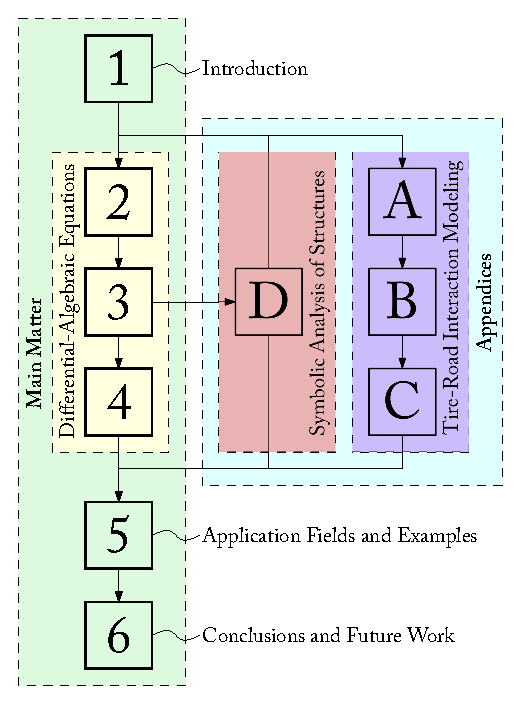
\includegraphics[width=9cm]{./figures/chapter_1/thesis_flowchart}
  \caption{Flowchart of the thesis structure, illustrating the logical progression of the chapters and appendices.}
  \label{chap1:fig:thesis_flowchart}
\end{figure}

% % % % % % % % % % % % % % % % % % % % % % % % % % % % % % % % % % % % % % % %

%!TEX root = ../main.tex

\chapter{Symbolic Computation and Applications}
\label{chapter:symbolic_computation}

Il calcolo simbolico è particolarmente utile per risolvere problemi che coinvolgono manipolazioni simboliche di espressioni matematiche piuttosto che semplici valori numerici. Ecco alcuni esempi di problemi in cui il calcolo simbolico si rivela prezioso:

Derivazione e Integrazione Simbolica:
Esempio 1: Calcolare la derivata di una funzione complessa, come ad esempio .
Esempio 2: Eseguire l'integrazione simbolica di una funzione come
Algebra Simbolica:
Esempio 3: Semplificare espressioni algebriche comple
Esempio 4: Risolvere sistemi di equazioni lineari o non lineari in forma simbolica.
Equazioni Differenziali Ordinarie (EDO):
Esempio 5: Risolvere un'equazione differenziale come
Esempio 6: Trovare una soluzione generale per un sistema di EDO complesso.
Matrici e Algebra Lineare:
Esempio 7: Calcolare l'inversa di una matrice simbolica.
Esempio 8: Trovare gli autovalori e gli autovettori di una matrice.
Teoria dei Numeri:
Esempio 9: Effettuare manipolazioni simboliche con espressioni che coinvolgono numeri irrazionali o complessi.
Esempio 10: Sviluppare algoritmi simbolici per la fattorizzazione di numeri o espressioni.


Chiarisco che l'analisi numerica solitamente coinvolge metodi computazionali basati su calcoli approssimati piuttosto che manipolazioni simboliche. Tuttavia, ci sono situazioni in cui il calcolo simbolico può essere incorporato nell'analisi numerica per migliorarne l'efficienza o risolvere specifici sotto-problemi. Ecco alcuni esempi:

Analisi di Errore:
Utilizzare il calcolo simbolico per derivare formule esatte per l'errore di approssimazione in un determinato metodo numerico, ad esempio, nell'approssimazione di una derivata o di un'integrale.
Ottimizzazione di Algoritmi Numerici:
Incorporare il calcolo simbolico per semplificare e ottimizzare passaggi critici in algoritmi numerici, ad esempio, nell'ottimizzazione di formule iterative o nella semplificazione di espressioni complesse all'interno di algoritmi.
Generazione di Funzioni Approssimanti:
Utilizzare il calcolo simbolico per derivare esattamente la forma chiusa di una funzione approssimante, ad esempio, attraverso metodi di interpolazione, semplificando così i calcoli numerici successivi.
Stabilità Numerica:
Analizzare la stabilità di un algoritmo numerico utilizzando il calcolo simbolico per esaminare il comportamento asintotico delle espressioni coinvolte nel processo numerico.
Risoluzione di Problemi Lineari o Non-Lineari:
Utilizzare tecniche di calcolo simbolico per semplificare le espressioni prima di applicare metodi numerici, riducendo così il numero di operazioni computazionali e migliorando l'efficienza computazionale.
Rappresentazione Esatta di Numeri Irrazionali:
Utilizzare il calcolo simbolico per rappresentare in modo esatto numeri irrazionali coinvolti in un problema numerico, evitando così errori di approssimazione.
Analisi di Sensibilità:
Utilizzare il calcolo simbolico per derivare espressioni analitiche per la sensibilità di una soluzione numerica rispetto alle variazioni nei parametri di input.
In queste situazioni, il calcolo simbolico può essere un complemento utile all'analisi numerica, contribuendo a una migliore comprensione del problema e ottimizzando l'implementazione degli algoritmi computazionali.
%!TEX root = ../main.tex

\chapter[DAEs Index Reduction and Numerical Solution]{Differential-Algebraic Equations Index Reduction and Numerical Solution}
\label{chap3:daes}

In this chapter, we present an algorithm for the index reduction of first-order \acp{DAE}. The proposed approach can be applied to generic \acp{DAE} and exploits neither a priori knowledge nor ad hoc techniques to leverage the specific formulation of the system. The index reduction is performed only by using symbolic manipulation and linear algebra techniques. It is based on the successive separation of the differential and algebraic equations of the system and the subsequent differentiation of the algebraic part. Improved symbolic matrix factorization is used to perform the \acp{DAE} partitioning, ensure numerical stability, and limit the expression swell of the reduced-index system. The effectiveness of the algorithm will be validated in the next chapter through a set of examples on a wide range of systems, including physical systems, engineering applications, and ``artificial'' \acp{DAE} with specific properties. The proposed symbolic index reduction algorithm is implemented in \Maple{} as part of an open-source library.

% % % % % % % % % % % % % % % % % % % % % % % % % % % % % % % % % % % % % % % %

\section{Differential-Algebraic Equations Index Reduction and Solution}
\label{chap3:sec:introduction}

As we already mentioned in Chapter~\ref{chap1:introduction}, \acp{DAE} are extensively used in dynamic system modeling. The challenge in numerically solving a \ac{DAE} system is assessed through its differentiation index, commonly referred to as ``the'' index~\cite{campbell1995index, campbell1995highindex}. Achieving accurate simulations necessitates converting high-index \acp{DAE} into low-index counterparts, posing a well-recognized challenge~\cite{petzold1982differential}. This process involves transforming a \ac{DAE} system into an equivalent system with a lower index through successive differentiation of the system equations. For this reason, the differentiation index is roughly defined as the number of times algebraic equations are differentiated to obtain an equivalent system of \acp{ODE} with invariants. Index reduction is a crucial step prior to the numerical integration of \acp{DAE}, as integrating high-index systems can be impractical. The primary obstacle lies in the necessity to solve non-linear systems of equations at each integration step, which can be computationally expensive and, in certain cases, numerically unstable. Specific numerical techniques, introduced in~\cite{petzold1982differential, thomsen1999numerical, baumgarte1972stabilization}, have been developed to address this challenge. However, these methods are not universally effective and may be inapplicable to some high-index \acp{DAE}. Consequently, index reduction becomes an indispensable preliminary stage before numerical integration~\cite{lamour2013differential}.

Given its complicated nature, index reduction has been the subject of extensive research and is often carried out by leveraging the specific formulation of the \ac{DAE} system, like in the multi-body modeling~\cite{zhou2005implicit, zhou2007symbolic, zhou2007symbolicseq, bayo1988modified, wehage1982generalized}. When the specific formulation of the \ac{DAE} system is not known a priori, or the system is not in a specific form, the index reduction process becomes more challenging. Many current simulation software packages for dynamic systems use index-reduction algorithms based on the \ac{SA} of the system, such as the Pantelides algorithm~\cite{pantelides1988consistent} and the dummy derivatives method~\cite{mattsson1993index}, which are subcases of the Pryce's $\Sigma$-method~\cite{pryce1998solving, pryce2001simple, nedialkov2007solvingI, nedialkov2007solvingII, nedialkov2008solvingIII, nedialkov2015algorithm, tan2016symbolic, mckenzie2017structural}. These algorithms are effective in reducing the index of most of the systems, but they can fail either for numerical cancellations~\cite{iwata2019index} or underestimation of the differentiation index~\cite{pantelides1988consistent, unger1995structural}, like in the case of Rei{\ss}ig's \acp{DAE} family~\cite{reissig2000differential}. Symbolic manipulation is proven to be successful in restating a \acp{DAE} on which the $\Sigma$-method fails to a \acp{DAE} on which the \ac{SA} may succeed~\cite{tan2016symbolic}.

Index reduction based on symbolic-numeric aided \ac{SA} has been successful in handling failures of the Pryce's $\Sigma$-method~\cite{tan2016symbolic} as well as in performing symbolically-informed \ac{SA}~\cite{chowdhry2004symbolic}. This latter \ac{SA} approach, which is named $\sigma v$-method, uses symbolic-numeric \ac{LU} factorization for variable substitution and rank determination on linear constant coefficient \acp{DAE}. A valuable attempt to use pure symbolic manipulation in \acp{DAE} index reduction is presented in~\cite{zhou2005implicit, zhou2007symbolic, zhou2007symbolicseq}, where implicit involutive form and \ac{LU} decomposition are successfully used to reduce the index of a simple constrained multi-body system. It is clear that index reduction algorithms based on pure symbolic matrix factorization represent a viable alternative to classic \ac{SA} techniques. However, symbolic matrix factorization feasibility is strongly tied to the performance of the symbolic computation kernel and its capabilities~\cite{zhou2008fraction}. Large expressions can lead to strong performance degradation of the kernel. Techniques aimed at limiting this decrease of performance while performing symbolic linear algebra operations are presented in~\cite{zhou2006hierarchical, zhou2007symbolic, zhou2007symbolicseq}. In these works, the hierarchical representation of expressions is applied to matrix factorization tasks. Nonetheless, the \LULEM{} package~\cite{carette2006linear}, which implements large expression management strategies in \ac{LU} decomposition, significantly outperforms the \Maple{}'s built-in matrix factorization routines.

The absence of user-invocable standalone functions within the \Maple{} environment that allows for the automatic index reduction of \acp{DAE}, and the inability to extract both the reduced-index system and invariants from the \texttt{dsolve} function, are the primary motivations of this research. Furthermore, recent advances in symbolic matrix factorization, combined with expressions hierarchical representation techniques, provide valuable tools that enable us to further investigate the applicability of a novel algorithm for the index reduction of \ac{DAE} systems, firstly presented in~\cite{stocco2024symbolic} as a preliminary work. The proposed methodology is similar to the previous work of~\citet{chowdhry2004symbolic} and extends it to generic first-order \acp{DAE}, linear in the states' derivatives. Nonetheless, the proposed algorithm does not work on the structural matrix of the system but on the \ac{DAE} system symbolic expressions. Specifically, the idea of using matrix factorization for variable substitution and rank determination is adopted to iteratively separate the differential and algebraic equations of the system. The algebraic equations are then differentiated to obtain an equivalent system with a lower differentiation index. Not less important, new libraries for symbolic matrix factorization (\LAST{}), large expression management (\LEM{}), and signature computation (\SIG{}) are presented. These libraries are based on the \LULEM{} package and extend the work of~\citet{zhou2006hierarchical, carette2006linear} and~\citet{zhou2007symbolic}. The newly presented libraries are designed to ensure the numerical stability of the numerically evaluated expressions, limit the expression swell, and provide an updated object-oriented interface. The effectiveness of the presented index reduction algorithm is validated through symbolic-numerical examples on a wide range of systems, including physical systems, engineering applications, as well as ``artificial'' systems with specific properties. The proposed algorithm is implemented in the \Maple{} environment and is available as a collection of open-source packages~\cite{last, lem}. Furthermore, the insights and the techniques presented in~\cite{zhou2006hierarchical, carette2006linear, zhou2007symbolic} are used to improve the presented algorithm to embed the hierarchical representation of expressions in a future implementation of the algorithm.

%This chapter is organized as follows. After this introduction (Section~\ref{chap3:sec:introduction}), the index reduction algorithm is presented in Section~\ref{chap3:sec:algorithm}. The expression swell mitigation, as well as the details on the symbolic matrix factorization, are discussed in Sections~\ref{chap3:sec:expression_swell} and \ref{chap3:sec:matrix_factorization}. The effectiveness of the algorithm is showcased through symbolic-numerical examples in Section~\ref{chap3:sec:example}. Finally, Sections~\ref{chap3:sec:future_work} and~\ref{chap3:sec:conclusions} report future developments and conclusions respectively. In~\ref{chap3:sec:cokernel} details on cokernel computation are reported. The newly developed object-oriented symbolic linear algebra (\ref{chap2:sec:last}), large expression management (\ref{chap2:sec:lem}) and signature computation (\ref{chap3:sec:signature}) package descriptions are also included in the appendices. The symbolic index reduction algorithm is implemented in the \Maple{} language and is available as part of the open-source \Indigo{} library~\cite{indigo}. Its usage is illustrated in~\ref{chap3:sec:index_reduction}.

% % % % % % % % % % % % % % % % % % % % % % % % % % % % % % % % % % % % % % % %

\section{A New Index Reduction Algorithm}
\label{chap3:sec:algorithm}

In this section, we explore the theoretical aspect of reducing the differential index of \ac{DAE} systems. Specifically, to systematically reduce the \ac{DAE} system's index, a novel iterative algorithm is presented. This algorithm comprises two main phases: initially, the separation of the differential equations from the algebraic equations inherent in \acp{DAE}; and subsequently, the differentiation of the algebraic ones to obtain an equivalent system with a reduced index. The algorithm that is presented in this section is implemented in the \Maple{} environment and is available as an open-source package~\cite{indigo}.

\subsection{Differential and Algebraic Equations Separation}
\label{chap3:sec:separation}

The initial phase of the index reduction procedure involves the partitioning of the \ac{DAE} system into its differential and algebraic equations. While in the case of small systems this can be accomplished through manual identification and isolation of the algebraic equations, this approach is inconvenient when dealing with large systems. An alternative method for automating the separation process leverages the cokernel, or left null space, of the \ac{DAE} system matrix, which is computed through matrix factorization techniques. The usage of the cokernel offers a more efficient and reliable means of accomplishing the separation task, variable substitution and not less importantly rank determination.

Consider a first-order system of \acp{DAE} $\mF$ of the form
%
\begin{equation}
  \label{chap3:eq:daes}
  \mF = \mA \, \mxp - \mb = \m{0}.
\end{equation}
%
We denote the cokernel and its orthogonal complement of $\mA$ with $\mK$ and $\mN$ respectively (see~\ref{chap3:sec:cokernel} for details on the cokernel computation with symbolic matrix factorization). Notice that the cokernel is the subspace obtained by the span of $\mK$'s columns. For this reason, hereafter, we refer to the cokernel as the matrix $\mK$ whose columns span the cokernel. Using $\mK$ and $\mN$ it is possible to separate the algebraic part of the \acp{DAE}~\eqref{chap3:eq:daes} as
%
\begin{equation}
  \label{chap3:eq:separated_daes}
  \begin{cases}
    \mE \, \mxp = \mg \\[0.1em]
    \ma = \m{0}
  \end{cases} \text{,} \quad \text{where} \qquad \mA = \begin{bmatrix}
    \mE \\[0.2em]
    \m{0}
  \end{bmatrix} \text{,}
  \quad \text{and} \quad
  \mb = \begin{bmatrix}
     \mg \\[0.2em]
     \ma
  \end{bmatrix} \text{.}
\end{equation}
%
The separated equations of the \acp{DAE} are obtained by the left product of $\mK$ and $\mN$ as
%
\begin{equation}
  \begin{array}{l@{~}c@{~}l}
    \mE &=& \mN \, \mA \text{,} \\[0.1em]
    \mg &=& \mN \, \mb \text{,} \\[0.1em]
    \ma &=& \mK \, \mb \text{.}
  \end{array}
\end{equation}
%
This results in an equivalent \ac{DAE} system, where the algebraic equations $\ma$ are now explicit. The details of the cokernel and its orthogonal complement computation are discussed in~\ref{chap3:sec:cokernel}.


\subsubsection{Cokernel Computation with Matrix Factorization}
\label{chap3:sec:cokernel}

The cokernel of a generic matrix $\m{A}$ is denoted as $\m{K}$ and satisfy $\m{K}\m{A} = \m{0}$. As mentioned before, the cokernel is the subspace obtained by the span of $\m{K}$'s columns. The orthogonal complement of the cokernel is denoted as $\m{N}$, moreover, the matrices $\m{N}$ and $\m{K}$ stacked compose a square non-singular matrix. It is common knowledge that matrix factorization techniques can be employed to compute the cokernel and its orthogonal complement. Among these techniques, the \ac{LU} factorization stands out as one of the most frequently used methods.

\paragraph{Lower-Upper Decomposition}

The full-pivoting \ac{LU} decomposition of a matrix $\m{A} \in \mathbb{R}^{m \times n}$ (with $m\geq n$) is represented as the product of matrices $\m{L}$ and $\m{U}$ with the permutation matrices $\mP$ and $\mQ$. It is characterized by the following properties:
%
\begin{itemize}
  \setlength{\itemsep}{0.0em}
  \item $\mP\m{A}\mQ = \m{L}\m{U}$;
  \item $\m{L} \in \mathbb{R}^{m \times m}$ is a lower-triangular matrix with all diagonal entries equal to $1$;
  \item $\m{U} \in \mathbb{R}^{m \times n}$ is an upper-triangular matrix;
  \item $\mP \in \mathbb{R}^{m \times m}$ and $\mQ \in \mathbb{R}^{n \times n}$ are the rows and columns permutation matrices, respectively.
\end{itemize}
%
If $\m{M}$ is defined such that $\m{M} = \m{L}^{-1}\mP$, then the following relation holds
%
\begin{equation}
    \m{M}\m{A}
    = \m{L}^{-1}\mP\m{A}
    = \m{L}^{-1}\mP\m{A}\mQ\mQ^\top
    = \m{L}^{-1}\m{L}\m{U}\mQ^\top
    = \m{U}\mQ^\top
    = \begin{bmatrix} \m{U}_1 \\[0.2em] \m{0} \end{bmatrix}\mQ^\top \text{.}
\end{equation}
%
If the identity matrix $\mI$ is partitioned as
%
\begin{equation}
  \mI = \begin{bmatrix}
    \mI_1 & \m{0} \\[0.2em]
    \m{0} & \mI_2
  \end{bmatrix} \text{,}
  %
  \quad \text{where} \quad
  %
  \begin{array}{l}
    \mI_1 \in \mathbb{R}^{m \times m} \quad \text{and} \quad
    \mI_2 \in \mathbb{R}^{(m-n)\times(m-n)}\text{,}
  \end{array}
\end{equation}
%
we can write
%
\begin{equation}
  \begin{bmatrix} \mI_1 & \m{0} \end{bmatrix} \, \m{M}\m{A} =
  \begin{bmatrix} \mI_1 & \m{0} \end{bmatrix}
  \begin{bmatrix} \m{U}_1 \\[0.2em] \m{0} \end{bmatrix} \mQ^\top = \m{U}_1 \mQ^\top
  %
  , \qquad \text{and} \qquad
  %
  \begin{bmatrix} \m{0} & \mI_2 \end{bmatrix} \, \m{M}\m{A} =
  \begin{bmatrix} \m{0} & \mI_2 \end{bmatrix}
  \begin{bmatrix} \m{U}_2 \\[0.2em] \m{0} \end{bmatrix} \mQ^\top = \m{0} \text{.}
\end{equation}
%
Eventually, the matrices $\m{N}$ and $\m{K}$ have the following form
%
\begin{equation*}
  \m{N} = \begin{bmatrix} \mI_1 & \m{0} \end{bmatrix} \, \m{M}
  %
  \quad \text{and} \quad
  %
  \m{K} = \begin{bmatrix} \m{0} & \mI_2 \end{bmatrix} \, \m{M},
\end{equation*}
%
where
%
\begin{equation*}
  \begin{array}{l}
      \m{K}\m{A} = \m{0} \\[0.2em]
      \m{N}\m{A} = \m{U}_1 ~ \text{is full-rank}
  \end{array} \, \text{,}
  %
  \quad \text{and} \quad
  %
  \begin{bmatrix} \m{N} \\[0.2em] \m{K} \end{bmatrix} \quad \text{is non-singular.}
\end{equation*}

\paragraph{Fraction-Free Lower-Upper Decomposition}

The \ac{FFLU} factorization is a variant of the \ac{LU} decomposition. It is based on the same principles as the standard \ac{LU} decomposition, but it is designed to avoid the appearance of fractions in the intermediate results. Similarly to the \ac{LU} case, the \ac{FFLU} decomposition of a matrix $\m{A} \in \mathbb{R}^{m \times n}$ (with $m\geq n$) is represented as the quintet of matrices $\m{L}$, $\m{U}$, $\m{D}$, $\mP$, and $\mQ$, and is characterized by the properties:
%
\begin{itemize}
  \setlength{\itemsep}{0.0em}
  \item $\mP\m{D}\m{A}\mQ = \m{L}\m{U}$;
  \item $\m{L} \in \mathbb{R}^{m \times m}$ is a lower-triangular matrix with all diagonal entries equal to $1$;
  \item $\m{D} \in \mathbb{R}^{m \times m}$ is a diagonal matrix;
  \item $\m{U} \in \mathbb{R}^{m \times n}$ is an upper-triangular matrix;
  \item $\mP \in \mathbb{R}^{m \times m}$ and $\mQ \in \mathbb{R}^{n \times n}$ are the rows and columns permutation matrices, respectively.
\end{itemize}
%
The procedure for computing the cokernel of a matrix $\m{A}$ using the \ac{FFLU} is similar to the case of the \ac{LU} decomposition. The only difference is in the computation of the matrix product $\m{M}\m{A}$. If $\m{M} = \m{L}^{-1}\mP\m{D}$, then $\m{M}\m{A}$ are written as
%
\begin{equation}
  \m{M}\m{A}
  = \m{L}^{-1}\mP\m{D}\m{A}
  = \m{L}^{-1}\mP\m{D}\m{A}\mQ\mQ^\top
  = \m{L}^{-1}\m{L}\m{U}\mQ^\top
  = \m{U}\mQ^\top = \begin{bmatrix} \m{U}_1 \\[0.2em] \m{0} \end{bmatrix}\mQ^\top \text{.}
\end{equation}
%
Then, the subspaces $\m{N}$ and $\m{K}$ are computed as in the \ac{LU} case.

\subsection{Algebraic Equations Differentiation}
\label{chap3:sec:differentiation}

The algebraic equations in the \ac{DAE} system~\eqref{chap3:eq:separated_daes} are now differentiated as
%
\begin{equation}
  \label{chap3:eq:diff_daes}
  \dfrac{\mathrm{d}}{\mathrm{d}t} \ma = \mAd \, \mxp - \mgd \text{.}
\end{equation}
%
The \acp{DAE}~\eqref{chap3:eq:separated_daes} after differentiation of algebraic equations now take a form similar to that of~\eqref{chap3:eq:daes}, where
%
\begin{equation}
  \label{chap3:eq:reduced_daes}
  \mA = \begin{bmatrix} \mE \\[0.2em] \mAd\end{bmatrix} \text{,}
  \quad \text{and} \quad
  \mb = \begin{bmatrix} \mg \\[0.2em] \mgd\end{bmatrix} \text{.}
\end{equation}
%
The set of invariants, which are collected in $\mh$, is updated adding the algebraic equations $\ma$
%
\begin{equation}
  \mh \quad \xleftarrow[\text{update}]{\text{\, Invariants \,}} \quad \overset{{\text{The old $\mh$}}}{\begin{bmatrix} \overbrace{\mh} \\[0.2em] \ma \end{bmatrix}} \text{.}
\end{equation}
%
The iterative procedure, involving the sequential separation and differentiation of the algebraic segment of the system, is iterated until $\mA$ is non-singular. When $\mA$ is non-singular the \ac{DAE} corresponds to a system of \acp{ODE} compounded by the invariants $\mh$, which are the collection of the hidden constraints produced in the index reduction process. The invariants $\mh$ can be initialized empty or with user-defined algebraic equations aimed at preserving crucial system properties, such as energy conservation and/or momentum conservation. A pseudocode of the index reduction algorithm can be found in Algorithm~\ref{chap3:alg:index_reduction}.

\begin{breakablealgorithm}
  \caption{Index reduction algorithm (without large expression management)~\cite{stocco2024symbolic}.}
  \label{chap3:alg:index_reduction}
  \begin{algorithmic}[1]
    \State \textbf{Require:} A \ac{DAE} system of the form $\mF \eqdef \mA \, \mxp - \mb = \m{0}$.
    \Procedure{ReduceIndex}{$\mF$} \Comment{Index reduction procedure}
      \State $\mh \gets \varnothing$ \Comment{The set of invariants}
      \State $\mA, \, \mb \gets \mathrm{GenerateMatrix}(\mF, \, \mxp)$ \Comment{The \ac{DAE} system matrix}
      \State $m \gets \mathrm{Size}(\mx)$\Comment{The size of $\mx$}
      \While{$\mA$ is singular}
        \State $\displaystyle\triangleright$ Differential and algebraic equations separation (Section~\ref{chap3:sec:separation})
        \State $\mL, \, \mU, \, \mP, \, \mQ \gets \mathrm{MatrixFactorization}(\mA)$ \Comment{LU or FFLU decomposition of $\mA$}
        \State $r \gets \mathrm{Rank}(\mU)$ \Comment{The rank of $\mU$ is equal to the rank of $\mA$}
        \State $\mI_1 \gets \mathrm{IdentityMatrix}(r, \, r)$ \Comment{The upper identity matrix}
        \State $\mI_2 \gets \mathrm{IdentityMatrix}(m-r, \, m-r)$ \Comment{The lower identity matrix}
        \State $\mE \gets \begin{bmatrix} \mI_1, \, \m{0} \end{bmatrix} \, \mU \, \mQ^\top$ \Comment{The reordered part of $\mA$}
        \State $\mg \gets \begin{bmatrix} \mI_1, \, \m{0} \end{bmatrix} \, \mL^{-1} \, \mP \, \mb$ \Comment{The differential part of $\mb$}
        \State $\ma \gets \begin{bmatrix} \m{0}, \, \mI_2 \end{bmatrix} \, \mL^{-1} \, \mP \, \mb$ \Comment{The algebraic part of $\mb$}
        \State $\displaystyle\triangleright$ Algebraic equations differentiation (Section~\ref{chap3:sec:differentiation})
        \State $\mAd, \, \mgd \gets \mathrm{GenerateMatrix}(\mathrm{Diff}(\ma, \, t), \, \mxp)$ \Comment{Differentiate the equations $\ma$}
        \State $\mA \gets \begin{bmatrix} \mE \\ \mAd \end{bmatrix}$ and $\mb \gets \begin{bmatrix} \mg \\ \mgd \end{bmatrix}$
        \Comment{The new matrix $\mA$ and vector $\mb$}
        \State $\mh \gets \mh \cup \ma$ \Comment{Add the algebraic equations to the set of invariants}
      \EndWhile \\
      \Return $\mA, \, \mb, \, \mh$ \Comment{The \acp{DAE} reduced to an \ac{ODE} system with invariants}
    \EndProcedure
  \end{algorithmic}
\end{breakablealgorithm}

\subsection{A Step-by-Step Example}
\label{chap3:sec:step_by_step}

Within this Section, we present the step-by-step results of the index reduction algorithm. To do so we exploit a simple non-stiff index-3 problem found in \Wolfram{}~\Mathematica{} documentation~\cite{mathematica}. The initial value problem is defined as follows
%
\begin{equation}
  \label{chap3:eq:index_3}
  \mF = \begin{bmatrix}
    x^{\prime}_{2} - x_{1} - \cos(t) \\
    x^{\prime}_{3} - x_{2} - \sin(t) \\
    x_{3} - \cos(t)
  \end{bmatrix},
\end{equation}
%
with states $\mx = [x_{1}, \, x_{2}, \, x_{3}]^\top$ and initial conditions $\mx_{0} = [-1, \, 0, \, 1]^\top$. Notice that the analytical solution of this problem is $\mx_\text{exact} = [\sin(t) - 2\cos(t), \, 2\sin(t), \, \cos(t)]^\top$. The index reduction algorithm is applied to the \ac{DAE} system~\eqref{chap3:eq:index_3} and the step-by-step results for the matrices $\mE$, $\mg$, and $\ma$ are reported here below.
%
\begin{equation*}
  \begin{array}{l}
    \text{Index-3 \acp{DAE}:} \quad \mE = \begin{bmatrix}
      0 & 1 & 0 \\
      0 & 0 & 1
    \end{bmatrix}, \quad
    \mg = \begin{bmatrix}
      \sin(t) - x_{1} \\
      \sin(t) - x_{2}
    \end{bmatrix}, \quad
    \ma = \begin{bmatrix}
      \cos(t) - x_{3}
    \end{bmatrix}. \\[1.0em]
    %
    \text{Index-2 \acp{DAE}:} \quad \mE = \begin{bmatrix}
      0 & 1 & 0 \\
      0 & 0 & 1
    \end{bmatrix}, \quad
    \mg = \begin{bmatrix}
      \sin(t) - x_{1} \\
      \sin(t) - x_{2}
    \end{bmatrix}, \quad
    \ma = \begin{bmatrix}
      2\sin(t) - x_{2}
    \end{bmatrix}. \\[1.0em]
    %
    \text{Index-1 \acp{DAE}:} \quad \mE = \begin{bmatrix}
      0 & 0 & 1 \\
      0 & 1 & 0
    \end{bmatrix}, \quad
    \mg = \begin{bmatrix}
      \sin(t) - x_{2} \\
      \sin(t) - x_{1}
    \end{bmatrix}, \quad
    \ma = \begin{bmatrix}
      \sin(t) - 2\cos(t) - x_{1}
    \end{bmatrix}. \\[1.0em]
    %
    \text{Index-0 \acp{DAE}:} \quad \mE = \begin{bmatrix}
      0 & 0 & 1 \\
      0 & 1 & 0 \\
      1 & 0 & 0
    \end{bmatrix}, \quad
    \mg = \begin{bmatrix}
      \sin(t) - x_{2} \\
      \sin(t) - x_{1} \\
      2\sin(t) + \cos(t)
    \end{bmatrix}, \quad
    \ma = \varnothing.
  \end{array}
\end{equation*}
%
The final form of the system is an index-0 \acp{DAE} system is then
%
\begin{equation}
  \label{chap3:eq:index_3_reduced}
  \mF = \begin{bmatrix}
    x^{\prime}_{2} - x_{1} - \cos(t) \\
    x^{\prime}_{3} - x_{2} - \sin(t) \\
    x^{\prime}_{1} - \cos(t) - 2\sin(t)
  \end{bmatrix},
  %
  \quad \text{with invariants} \quad
  %
  \mh = \begin{bmatrix}
    \cos(t) - x_{3} \\
    2\sin(t) - x_{2} \\
    \sin(t) - 2\cos(t) - x_{1}
  \end{bmatrix}.
\end{equation}
%
Although the just presented example is not so complex and relevant for a real validation of the algorithm, it is useful to demonstrate the step-by-step results of the index reduction algorithm. Furthermore, the expression complexities encountered throughout the index reduction algorithm applied to the Index-3 problem are reported below in \tablename{}~\ref{chap3:tab:index_3}.

\begin{table}
  \caption{Expression complexity encountered throughout the index reduction of the index-3 step-by-step example problem~\cite{mathematica} \ac{DAE} system index reduction. \emph{Legend}: $\cf$ = functions, $\ca$ = additions, $\cm$ = multiplications, and $\cd$ = divisions.}
  \label{chap3:tab:index_3}
  \centering
  {\footnotesize\begin{tabular}{cccc}
    \multicolumn{4}{c}{\textbf{Index-3 \acp{DAE}~\cite{mathematica}}} \\
    \toprule
    \textbf{Original \acp{DAE}} & \multicolumn{3}{c}{$\mF = 10\cf + 5\ca$ \quad $\mh = 0$} \\
    \midrule
    \textbf{Reduction step} & $\mE$ & $\mg$ & $\ma$ \\
    \midrule
    Index-3 \acp{DAE} & $0$ & $4\cf + 2\ca$ & $2\cf + 1\ca$ \\
    Index-2 \acp{DAE} & $0$ & $4\cf + 2\ca$ & $2\cf + 1\cm + 1\ca$ \\
    Index-1 \acp{DAE} & $0$ & $4\cf + 2\ca$ & $3\cf + 1\cm + 1\ca$ \\
    Index-0 \acp{DAE} & $0$ & $6\cf + 1\cm + 3\ca$ & $0$ \\
    \midrule
    \textbf{Reduced \acp{DAE}} & \multicolumn{3}{c}{$\mF = 12\cf + 1\cm + 6\ca$ \quad $\mh = 7\cf + 2\cm + 4\ca$} \\
    \bottomrule
    \end{tabular}}
\end{table}

\subsection{Acknowledging some Algorithm Limitations}

While the algorithm just presented is relatively straightforward to implement, it does have two major sources of potential issues that are both determined by the technology used and the fundamental theory.
%
\begin{itemize}
    \item \emph{Expression complexity}. Symbolic manipulation often leads to a growth in expression complexity. For this reason, expression simplification may not always be feasible due to software limitations or excessive CPU time demands. Making the algorithm insensitive to expression swell is thus crucial to its effectiveness.
    \item \emph{Numerical stability of symbolic matrix factorization}. The description of the algorithm involves the manipulation of matrices and vectors with either symbolic or mixed symbolic-numeric entries. Ensuring that symbolic matrix factorization maintains numerical stability is a critical requirement of the algorithm. In the case of \ac{LU} decomposition, inadequate pivoting strategies can lead to the generation of singular matrices, which in turn can cause the algorithm to fail~\cite{zhou2005implicit, zhou2007symbolic, giesbrecht2014symbolic}.
\end{itemize}
%
These are the two main points that we acknowledge in the implementation of the algorithm. In the forthcoming sections, each of these matters is discussed in detail, with recommendations on techniques and open-source software solutions that are used to address them.

\section{Index Reduction Algorithm with Expression Swell Mitigation}

The most interesting and relevant aspect to be explored is the connection between the hierarchical representation of expressions (see Section~\ref{chap2:sec:lem}) and the \ac{DAE} index reduction. The use of veiling variables may be used to hide some parts of the expressions by the collection of common sub-expressions. Even if this may appear to be a substantial improvement, it is not so frequent to encounter expressions that are common to all the equations of the \ac{DAE} system. Still, this concept can be extended to mitigate the expression swell during matrix factorization (see Section~\ref{chap2:sec:last}). The veiling variables $\mv$ would then include the states $\mx$ of the \ac{DAE} system. In this manner, the hierarchical representation of the expression serves as a system augmentation technique as well as a means to limit expression swell during the index reduction procedure. The augmented \ac{DAE} system would then be expressed as
%
\begin{equation}
  \label{chap3:eq:augmented_dae}
  \mFv = \mAv \, \mx^\prime - \mbv = \m{0},
  %
  \qquad \text{where} \qquad
  %
  \mv = \begin{bmatrix}
    v_{1}(\mx, t) \\
    v_{2}(v_{1}, \mx, t) \\
    \vdots \\
    v_{n}(v_{1}, \dots, v_{n-1}, \mx, t) \\
  \end{bmatrix}.
\end{equation}
%
Notice that if the matrix $\mAv$ is non-singular, the augmented \ac{DAE} system~\eqref{chap3:eq:augmented_dae} has index-1. This is a crucial aspect to be taken into consideration since, as demonstrated in Section~\ref{chap3:sec:daes_complexity}, the final reduction to index-0 \acp{DAE} is costly. Furthermore, the vector $\mv$ and its Jacobian with respect to the states $\mx$ can be sequentially evaluated for additional reduction of the computational burden. Nonetheless, the augmented formulation~\eqref{chap3:eq:augmented_dae} allows for the full exploitation of the signature technique to detect null expressions without the need for symbolic simplification~\cite{monagan1994signature}. Eventually, this will be the subject of future research and implementations that will exploit index-1 \acp{DAE} integrators similarly to the other state-of-the-art \acp{DAE} solver presented in the Introduction. A pseudocode and a flowchart of the index reduction algorithm with expression swell mitigation can be found in Algorithm~\ref{chap3:alg:index_reduction_veil} and \figurename~\ref{chap3:fig:index_reduction_veil}, respectively.

\begin{figure}[htp]
  \centering
  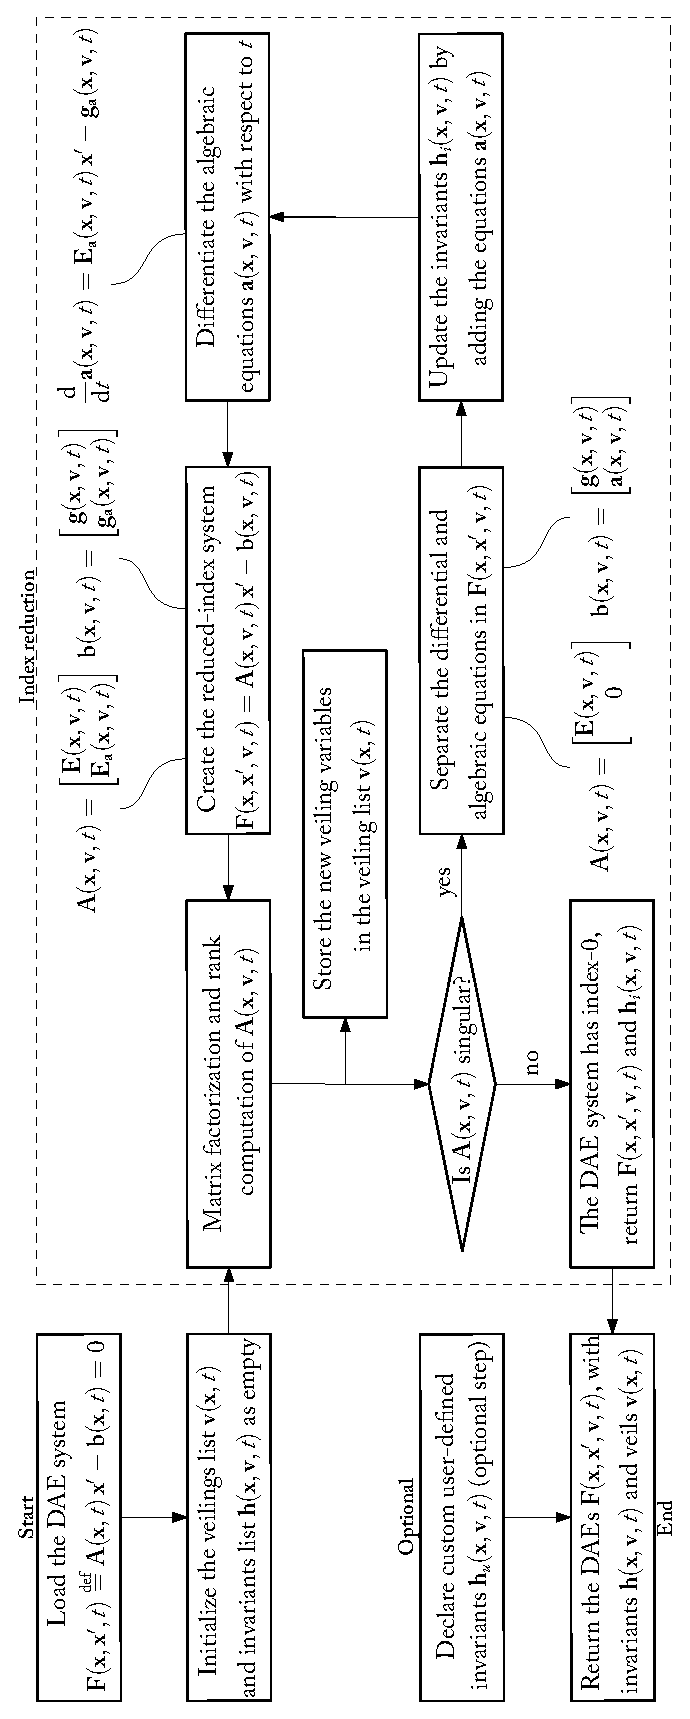
\includegraphics[angle=0, width=0.5\columnwidth]{dae_flowchart_veil}
  \caption{Flowchart of the index reduction algorithm with expression swell mitigation.}
  \label{chap3:fig:index_reduction_veil}
\end{figure}

\begin{breakablealgorithm}
  \caption{Index reduction algorithm with expression swell mitigation.}
  \label{chap3:alg:index_reduction_veil}
  \begin{algorithmic}[1]
    \State \textbf{Require:} A \ac{DAE} system of the form $\mFv \eqdef \mAv \, \mxp - \mbv = \m{0}$.
    \Procedure{ReduceIndex}{$\mFv$} \Comment{Index reduction procedure}
      \State $\mhiv \gets \varnothing$ \Comment{The set of invariants}
      \State $\mv \gets \varnothing$ \Comment{The veiling variables vector}
      \State $\mAv, \, \mbv \gets \mathrm{GenerateMatrix}(\mFv, \, \mxp)$ \Comment{The \ac{DAE} system matrix}
      \State $m \gets \mathrm{Size}(\mx)$\Comment{The size of $\mx$}
      \While{$\mAv$ is singular}
        \State $\displaystyle\triangleright$ Differential and algebraic equations separation (Section~\ref{chap3:sec:separation})
        \State $\mLv, \, \mUv, \, \mP, \, \mQ, \, \m{v}_d(\mx, \m{v}, \, t) \gets \mathrm{MatrixFactorization}(\mAv)$ \Comment{\ac{LU} or \ac{FFLU} decomposition of $\mAv$ with new veiling variables $\m{v}_d(\mx, \m{v}, \, t)$}
        \State $\mv \gets \mv \cup \m{v}_d(\mx, \m{v}, \, t)$ \Comment{Update the veiling variables vector}
        \State $r \gets \mathrm{Rank}(\mUv)$ \Comment{The rank of $\mUv$ is equal to the rank of $\mAv$}
        \State $\mI_1 \gets \mathrm{IdentityMatrix}(r, \, r)$ \Comment{The upper identity matrix}
        \State $\mI_2 \gets \mathrm{IdentityMatrix}(m-r, \, m-r)$ \Comment{The lower identity matrix}
        \State $\mEv \gets \begin{bmatrix} \mI_1, \, \m{0} \end{bmatrix} \, \mUv \, \mQ^\top$ \Comment{The reordered part of $\mAv$}
        \State $\mgv \gets \begin{bmatrix} \mI_1, \, \m{0} \end{bmatrix} \, \mLv^{-1} \, \mP \, \mbv$ \Comment{The differential part of $\mbv$}
        \State $\mav \gets \begin{bmatrix} \m{0}, \, \mI_2 \end{bmatrix} \, \mLv^{-1} \, \mP \, \mbv$ \Comment{The algebraic part of $\mbv$}
        \State $\displaystyle\triangleright$ Algebraic equations differentiation (Section~\ref{chap3:sec:differentiation})
        \State $\jac{\m{v}}{\mx}(\mx, \m{v}, \, t) \gets \mathrm{Jacobian}(\mv, \, \mx)$ \Comment{The Jacobian of $\mav$ with respect to $\mx$}
        \State $\mav \gets \mathrm{Diff}(\mav, \, t)$ \Comment{Differentiate the equations $\mav$}
        \State $\mav \gets \mathrm{Substitute}(\jac{\m{v}}{\mx}(\mx, \m{v}, \, t), \mav)$ \Comment{Remove the $\mv$ derivatives from $\mav$}
        \State $\mAdv, \, \mgdv \gets \mathrm{GenerateMatrix}(\mav, \, \mxp)$ \Comment{Differentiate the equations $\mav$}
        \State $\mAv \gets \begin{bmatrix} \mEv \\ \mAdv \end{bmatrix}$ and $\mbv \gets \begin{bmatrix} \mgv \\ \mgdv \end{bmatrix}$
        \Comment{The new matrix $\mAv$ and vector $\mbv$}
        \State $\mhiv \gets \mhiv \cup \mav$ \Comment{Add the algebraic equations to the set of invariants}
      \EndWhile \\
      \Return $\mAv, \, \mbv, \, \mhiv, \, \mv$ \Comment{The \acp{DAE} reduced to an \ac{ODE} system with invariants}
    \EndProcedure
  \end{algorithmic}
\end{breakablealgorithm}

% % % % % % % % % % % % % % % % % % % % % % % % % % % % % % % % % % % % % % % %

\section{Index Reduction and Numerical Integration Scheme}
\label{chap3:sec:indigo}

After this fairly long discussion on the actual implementation aspects of the index reduction algorithm, we can now present the \Indigo{} index reduction and integration toolbox~\cite{indigo}. This toolbox consists of two main components: a \Maple{} package to carry out symbolic index reduction of \ac{DAE} systems, and a \Matlab{} toolbox to perform numerical integration of the reduced-index system. \Indigo{} is designed to be used in conjunction with the \LEM{} package, to limit the expression swell, and the \LAST{} package, to conveniently factorize matrices. In the following paragraphs, we briefly discuss the usage of the \Indigo{} package.

\subsection{Index Reduction}

The index reduction algorithm implemented in the \Indigo{} \Maple{} package is the one presented in Section~\ref{chap3:sec:algorithm}. To reduce the index of a \ac{DAE} system in the \Maple{} environment we need to first create an \Indigo{} object instance.
%
\begin{verbatim}
> Indigo_obj := Object(Indigo);
> Indigo_obj:-InitLAST();
\end{verbatim}
%
Then, the system of \acp{DAE} \texttt{eqns} with coordinates \texttt{vars} is loaded.
%
\begin{verbatim}
> Indigo_obj:-LoadEquations('Generic', eqns, vars);
\end{verbatim}
%
The \texttt{Generic} symbol is used to specify the type of the system. Notice that in this example, we assume that the equations of the system are already available in the \Maple{} session. The automatic index reduction process can be performed by calling the \texttt{ReduceIndex} method, which iterates the separation and differentiation steps until an index-$0$ \ac{DAE} system is obtained.
%
\begin{verbatim}
> Indigo_obj:-ReduceIndex();
\end{verbatim}
%
Intermediate results of the process are stored internally in the \Indigo{} object and are available on demand. Once the index reduction process is completed, the user can generate the \texttt{SliderCrank} \Matlab{} class file to perform numerical integration of the reduced-index system.
%
\begin{verbatim}
> Indigo_obj:-GenerateMatlabCode(name, type, data=pars);
\end{verbatim}
%
A file \texttt{name.m} is generated in the current directory. As it is explained in the next section, The string parameter \texttt{type} can be either \texttt{Implicit}, \texttt{SemiExplicit} or \texttt{Explicit} depending on the desired numerical integration scheme. The optional parameter \texttt{data} introduces default internal object data.

\subsection{Numerical Integration Scheme}

The \Indigo{} \Matlab{} toolbox is an object-oriented library that allows the user to exploit the automatically generated code of the reduced-index system. It is capable of integrating systems of \acp{ODE} and \acp{DAE} using a variety of Runge-Kutta numerical integration schemes. In particular, the system of equations which is integrated is composed of the following elements.
%
\begin{itemize}
  \setlength{\itemsep}{0pt}
    \item A differential part, which can be expressed by one of the following classes:
    %
    \begin{equation}
        \begin{array}{ccl}
            \m{F}(\mx, \mx^\prime, \m{v}, t) = \m{0} & \hspace{0.5cm} &
            \text{\texttt{Implicit} system class,} \\[0.5mm]
            \m{A}(\mx, \m{v}, t) \, \mx^\prime = \m{b}(\mx, \m{v}, t) & \hspace{0.5cm} &
            \text{\texttt{SemiExplicit} system class,} \\[0.5mm]
            \mx^\prime = \m{f}(\mx, \m{v}, t) & \hspace{0.5cm} &
            \text{\texttt{Explicit} system class.}
        \end{array}
    \end{equation}
    %
    \item The invariants, composed of the hidden constraints obtained from the index reduction process $\mhiv$, and optional user-defined invariants $\mhuv$, namely
    %
    \begin{equation}
        \label{chap3:eq:inv_part}
        \m{h}(\mx, \m{v}, t) = \begin{bmatrix}
            \mhiv \\[0.5mm]
            \mhuv
        \end{bmatrix} = \m{0} \text{.}
    \end{equation}
    %
    \item The veils, which are the set of the expression hierarchical representation variables used in \LEM{} to limit the expression swell
    %
    \begin{equation}
        \m{v}(\mx, t) = \begin{bmatrix}
            v_{1}(\mx, t) \\[0.5mm]
            v_{2}(v_{1}, \mx, t) \\
            \vdots \\
            v_{n}(v_{1}, \dots, v_{n-1}, \mx, t)
        \end{bmatrix} \text{.}
    \end{equation}
\end{itemize}

To respect the invariants during the integration the \emph{standard projection} method is applied~\cite{hairer2000symmetric}. This method consists of projecting the solution $\mx$ of the numerically integrated reduced-index system onto the invariants manifold $\m{h}(\mx, \m{v}, t) = \m{0}$, which is equivalent to the following constrained minimization
%
\begin{equation}
  \underset{\widetilde{\mx}}{\textrm{minimize}} \quad \dfrac{1}{2}\left(\mx - \widetilde{\mx}\right)^2
    \quad \textrm{subject to} \quad
    \m{h}(\mx, \m{v}, t) = \m{0}.
\end{equation}

To integrate the system generated through the \Matlab{} package or a custom system \texttt{sys}, the user must first instantiate a \Indigo{} Runge-Kutta solver.
%
\begin{verbatim}
>>> solver = IndigoSolver('solver_name');
>>> solver.set_system(sys);
\end{verbatim}
%
Once the solver is instantiated, it is only necessary to specify the initial conditions and the integration time vector.
%
\begin{verbatim}
>>> [x, t, v, h] = solver.solve(t_ini:d_t:t_end, ics);
\end{verbatim}
%
The solver returns the solution of the system in the form of multiple outputs: \texttt{x} contains the integrated solution, \texttt{x\_dot} the states' time derivative, \texttt{t} the time vector, \texttt{v} the veiling variables, and finally \texttt{h} the values of the invariants over the specified time mesh \texttt{t\_ini:d\_t:t\_end}.

% % % % % % % % % % % % % % % % % % % % % % % % % % % % % % % % % % % % % % % %

\section{Proofing the Symbolic-Numeric Scheme}
\label{chap3:sec:example}

In this section, we showcase an example of a high-index \ac{DAE} system: an index-3 problem with an analytical solution, which describes the motion of a particle on a 3D torus surface~\cite{campbell1995constraint}. This example is employed to validate the numerical stability of the reduced-index system, as well as the good conditioning of both the symbolic matrix factorization and the numerical integration scheme. To ease the understanding of the results, we purposely avoid the use of the veiling variables in this example. However, the veiling variables just add an evaluation layer to the expressions, and they do not affect the numerical stability of the algorithm.

\subsection{Expression Complexity of the Reduced-Index Systems}
\label{chap3:sec:daes_complexity}

As a first demonstration of the proposed index reduction algorithm capabilities, we first consider the given example from a purely symbolic perspective. In particular, we consider the computational cost of the expressions generated during the presented procedure. The compactness of the expressions generated during the index reduction algorithm is a crucial aspect, as it ensures that limited computational overhead is introduced in the numerical integration of the reduced-index system, as well as in the projection of the solution on the hidden constraints. Specifically, the index reduction algorithm is applied to the \ac{DAE} system and reduced to index-0. For each reduction stage of the example considered, the computational cost is reported in \tablename{}~\ref{chap3:tab:torus}.

\begin{table}[htp]
  \caption{Expression complexity encountered throughout the index reduction of the robotic arm problem~\cite{brenan1995numerical} \ac{DAE} system index reduction. \emph{Legend}: $\cf$ = functions, $\ca$ = additions, $\cm$ = multiplications, and $\cd$ = divisions.}
  \label{chap3:tab:torus}
  \centering
  {\footnotesize\begin{tabular}{cccc}
    \multicolumn{4}{c}{\textbf{Particle Motion~\cite{campbell1995constraint}}} \\
    \toprule
    \textbf{Original \acp{DAE}} & \multicolumn{3}{c}{$\mF = 47\cf + 30\cm + 23\ca$ \quad $\mh = 0$} \\
    \midrule
    \textbf{Reduction step} & $\mE$ & $\mg$ & $\ma$ \\
    \midrule
    Index-3 \acp{DAE} & $0$ & $39\cf + 36\cm + 13\ca$ & $7\cf + 10\cm + 6\ca$ \\
    Index-2 \acp{DAE} & $0$ & $39\cf + 36\cm + 13\ca$ & $22\cf + 20\cm + 8\ca$ \\
    Index-1 \acp{DAE} & $0$ & $39\cf + 36\cm + 13\ca$ & $68\cf + 72\cm + 33\ca$ \\
    Index-0 \acp{DAE} & $388\cf + 424\cm + 180\ca$ & $79\cf + 77\cm + 26\ca$ & $0$ \\
    \midrule
    \textbf{Reduced \acp{DAE}} & \multicolumn{3}{c}{$\mF = 258\cf + 239\cm + 109\ca$ \quad $\mh = 97\cf + 102\cm + 47\ca$} \\
    \bottomrule
    \end{tabular}}
\end{table}

\subsection{Numerical Integration of the Reduced-Index System}
\label{chap3:sec:numerical_integration}

The numerical stability and consistency of the reduced-index system are demonstrated by exploiting the analytical solution of the problem in~\cite{campbell1995constraint}. Specifically, the \ac{DAE} system consists of three position variables $[x_{1}, \, x_{2}, \, x_{3}]^\top$, three velocity variables $[u_{1}, \, u_{2}, \, u_{3}]^\top$, and one constraint with Lagrange multiplier $\lambda$. The solution manifold is 4D, and the exact solution is
%
\begin{equation}
  \label{chap3:eq:torus_solution}
  \mx_\text{exact} = \begin{bmatrix}
    x_{1} \\ x_{2} \\ x_{3}
  \end{bmatrix} = \begin{bmatrix}
    (\rho \cos(2\pi - t) + r) \cos(t) \\
    (\rho \cos(2\pi - t) + r) \sin(t) \\
    \rho \sin(2\pi - t)
  \end{bmatrix} \, \text{.}
\end{equation}
%
The initial value problem is defined as follows
%
\begin{equation}
  \label{chap3:eq:torus}
  \mF = \begin{bmatrix}
    x^{\prime}_{1} - u_{1} \\
    x^{\prime}_{2} - u_{2} \\
    x^{\prime}_{3} - u_{3} \\
    u^{\prime}_{1} - u_{3}\cos(t) + x_{3}\sin(t) + u_{2} - 2 c x_{1}\lambda \\
    u^{\prime}_{2} - u_{3}\sin(t) - x_{3}\cos(t) - u_{1} - 2 c x_{2}\lambda \\
    u^{\prime}_{3} + x_{3} - 2x_{3}\lambda \\
    x_{1}^2 + x_{2}^2 + x_{3}^2 - 2r(x_{1}^2 + x_{2}^2)^{1/2} + r^2 - \rho^2
  \end{bmatrix} \, \text{,}
\end{equation}
%
with $c = 1 - {r} / {(x_{1}^2 + x_{2}^2)^{1/2}}$, states $\mx = [x_{1}, \, x_{2}, \, x_{3}, \, u_{1}, \, u_{2}, \, u_{3}, \, \lambda]^{\top}$, initial conditions $\mx_{0} = [15, \, 0, \, 0, \, 0, \, 15, \, -5, \, \lambda]^{\top}$, and parameters $\rho = 5$ and $r = 10$.

The numerical integration of the reduced-index system is performed through Implicit Euler, RadauIIA3, and RadauIIA5 Runge-Kutta methods. To respect the invariants during the integration the \emph{standard projection} method is applied~\cite{hairer2000symmetric}. This method consists of projecting the solution $\mx$ of the numerically integrated system onto the invariants on the hidden constraints $\mh = \m{0}$, which is equivalent to the constrained minimization
%
\begin{equation}
  \underset{\tilde{\mx}}{\textrm{minimize}} \quad \dfrac{1}{2}\left(\mx - \tilde{\mx}\right)^2
    \quad \textrm{subject to} \quad
    \mh = \m{0}.
\end{equation}
%
To verify that the projection is performed correctly and does not affect the order of the Runge-Kutta method, numerical integration is performed in the interval $t \in [0, \, 2\pi]$ seconds with different integration time steps $\Delta t$. The error of the numerical integration $\varepsilon = \| \, \mx - \mx_\text{exact} \, \|_{\infty}$ is reported in \figurename~\ref{chap3:fig:torus_order}. As can be seen, the implemented projection preserves the order of the method for all the integration time steps. It is important to highlight that to obtain such results the absolute error tolerances of the integrator and the projection are both set to $\varepsilon = 10^{-10}$. The same tolerances are used in the numerical integration of the reduced-index system in the interval $t \in [0, \, 400\pi]$ seconds with step $\Delta t = 0.025$ seconds. The results are reported in \figurename~\ref{chap3:fig:torus_integration}, where Implicit Euler, RadauIIA3, and RadauIIA5 Runge-Kutta methods are employed, and the projection on the hidden constraints $\mh$ is performed. The effect of the projection is highlighted on the bottom left plot.

\begin{figure}[htp]
  \centering
  \includetikz{figures/chapter_3/torus_order.tex}
  \includetikz{figures/chapter_3/torus_hidden.tex}
  \caption{Numerical integration error $\varepsilon = \| \, \mx - \mx_\text{exact} \, \|_{\infty}$ of the \acp{DAE}~\eqref{chap3:eq:torus} over different integration time steps $\Delta t$, along with the computed order of the method (left). The projection on the hidden constraints is performed and the invariants violation $\| \, \mh \, \|_{\infty}$ is reported (right). Notice that the implemented projection preserves the order of the method for all the integration time steps. The tests are performed in the interval $t \in [0, \, 2\pi]$ seconds, using Implicit Euler, RadauIIA3, and RadauIIA5 Runge-Kutta methods.}
  \label{chap3:fig:torus_order}
\end{figure}

\begin{figure}[htp]
  \centering
  \includetikz{figures/chapter_3/torus_implicit_euler.tex}
  \includetikz{figures/chapter_3/torus_radauiia3.tex}
  \includetikz{figures/chapter_3/torus_radauiia5.tex}
  \includetikz{figures/chapter_3/torus_radauiia5_noproj.tex}
  \caption{Numerically integrated solution of the \acp{DAE}~\eqref{chap3:eq:torus} in the interval $t \in [0, \, 400\pi]$ seconds, with step $\Delta t = 0.025$ seconds, using Implicit Euler (top left), RadauIIA3 (top right), and RadauIIA5 (bottom left and right) Runge-Kutta methods. The first three plots show the numerical integration of the reduced-index system with projection on the hidden constraints $\mh$ produced by the index reduction algorithm. On the bottom right plot, the numerical integration of the reduced-index system is performed without projection on the manifold $\mh$ and substantial drift is observed.}
  \label{chap3:fig:torus_integration}
\end{figure}

% % % % % % % % % % % % % % % % % % % % % % % % % % % % % % % % % % % % % % % %
%!TEX root = ../main.tex

\chapter[Solution of Dynamic Systems Described by DAEs]{Solution of Dynamic Systems Described by Differential-Algebraic Equations}
\label{chap4:daes}

In this chapter, we present an algorithm for the index reduction of first-order \acp{DAE}. The proposed approach can be applied to generic \acp{DAE} and exploits neither a priori knowledge nor ad hoc techniques to leverage the specific formulation of the system. The index reduction is performed only by using symbolic manipulation and linear algebra techniques. It is based on the successive separation of the differential and algebraic equations of the system and the subsequent differentiation of the algebraic part. Improved symbolic matrix factorization is used to perform the \acp{DAE} partitioning, ensure numerical stability, and limit the expression swell of the reduced-index system. The effectiveness of the algorithm will be validated in the next chapter through a set of examples on a wide range of systems, including physical systems, engineering applications, and ``artificial'' \acp{DAE} with specific properties. The proposed symbolic index reduction algorithm is implemented in \Maple{} as part of an open-source library.

% % % % % % % % % % % % % % % % % % % % % % % % % % % % % % % % % % % % % % % %

\section{Differential-Algebraic Equations Index Reduction and Solution}
\label{chap4:sec:introduction}

As we already mentioned in the previous chapters, \acp{DAE} are extensively used in dynamic system modeling. The challenge in numerically solving a \ac{DAE} system is assessed through its differentiation index, commonly referred to as ``the'' index~\cite{campbell1995index, campbell1995highindex}. Achieving accurate simulations necessitates converting high-index \acp{DAE} into low-index counterparts, posing a well-recognized challenge~\cite{petzold1982differential}. This process involves transforming a \ac{DAE} system into an equivalent system with a lower index through successive differentiation of the system equations. For this reason, the differentiation index is roughly defined as the number of times algebraic equations are differentiated to obtain an equivalent system of \acp{ODE} with invariants. Index reduction is a crucial step prior to the numerical integration of \acp{DAE}, as integrating high-index systems can be impractical. The primary obstacle lies in the necessity to solve nonlinear systems of equations at each integration step, which can be computationally expensive and, in certain cases, numerically unstable. Specific numerical techniques, introduced in~\cite{petzold1982differential, thomsen1999numerical, baumgarte1972stabilization}, have been developed to address this challenge. However, these methods are not universally effective and may be inapplicable to some high-index \acp{DAE}. Consequently, index reduction becomes an indispensable preliminary stage before numerical integration~\cite{lamour2013differential}.

Given its complicated nature, index reduction is the subject of extensive research and is often carried out by leveraging the specific formulation of the \ac{DAE} system, like in the multi-body modeling~\cite{zhou2005implicit, zhou2007symbolic, zhou2007symbolicseq, bayo1988modified, wehage1982generalized}. When the specific formulation of the \ac{DAE} system is not known a priori, or the system is not in a specific form, the index reduction process becomes more challenging. Many current simulation software packages for dynamic systems use index-reduction algorithms based on the \ac{SA} of the system, such as the Pantelides algorithm~\cite{pantelides1988consistent} and the dummy derivatives method~\cite{mattsson1993index}, which are subcases of the Pryce's $\Sigma$-method~\cite{pryce1998solving, pryce2001simple, nedialkov2007solvingI, nedialkov2007solvingII, nedialkov2008solvingIII, nedialkov2015algorithm, tan2016symbolic, mckenzie2017structural}. These algorithms are effective in reducing the index of most of the systems, but they can fail either for numerical cancellations~\cite{iwata2019index} or underestimation of the differentiation index~\cite{pantelides1988consistent, unger1995structural}, like in the case of Rei{\ss}ig's \acp{DAE} family~\cite{reissig2000differential}. Symbolic manipulation is proven to be successful in restating a \acp{DAE} on which the $\Sigma$-method fails to a \acp{DAE} on which the \ac{SA} may succeed~\cite{tan2016symbolic}.

Index reduction based on symbolic-numeric aided \ac{SA} has been successful in handling failures of the Pryce's $\Sigma$-method~\cite{tan2016symbolic} as well as in performing symbolically-informed \ac{SA}~\cite{chowdhry2004symbolic}. This latter \ac{SA} approach, which is named $\sigma v$-method, uses symbolic-numeric \ac{LU} factorization for variable substitution and rank determination on linear constant coefficient \acp{DAE}. A valuable attempt to use pure symbolic manipulation in \acp{DAE} index reduction is presented in~\cite{zhou2005implicit, zhou2007symbolic, zhou2007symbolicseq}, where implicit involutive form and \ac{LU} decomposition are successfully used to reduce the index of a simple constrained multi-body system. It is clear that index reduction algorithms based on pure symbolic matrix factorization represent a viable alternative to classic \ac{SA} techniques. However, symbolic matrix factorization feasibility is strongly tied to the performance of the symbolic computation kernel and its capabilities~\cite{zhou2008fraction}. Large expressions can lead to strong performance degradation of the kernel. Techniques aimed at limiting this decrease of performance while performing symbolic linear algebra operations are presented in~\cite{zhou2006hierarchical, zhou2007symbolic, zhou2007symbolicseq}. In these works, the hierarchical representation of expressions is applied to matrix factorization tasks. Nonetheless, the \LULEM{} package~\cite{carette2006linear}, which implements large expression management strategies in \ac{LU} decomposition, significantly outperforms the \Maple{}'s built-in matrix factorization routines.

The absence of user-invocable standalone functions within the \Maple{} environment that allows for the automatic index reduction of \acp{DAE}, and the inability to extract both the reduced-index system and invariants from the \texttt{dsolve} function, are the primary motivations of this research. Furthermore, recent advances in symbolic matrix factorization, combined with expressions hierarchical representation techniques, provide valuable tools that enable us to further investigate the applicability of a novel algorithm for the index reduction of \ac{DAE} systems, firstly presented in~\cite{stocco2024symbolic} as a preliminary work. The proposed methodology is similar to the previous work of~\citet{chowdhry2004symbolic} and extends it to generic first-order \acp{DAE}, linear in the states' derivatives. Nonetheless, the proposed algorithm does not work on the structural matrix of the system but on the \ac{DAE} system symbolic expressions. Specifically, the idea of using matrix factorization for variable substitution and rank determination is adopted to iteratively separate the differential and algebraic equations of the system. The algebraic equations are then differentiated to obtain an equivalent system with a lower differentiation index. Not less important, new libraries for symbolic matrix factorization (\LAST{}), large expression management (\LEM{}), and signature computation (\SIG{}) are presented. These libraries are based on the \LULEM{} package and extend the work of~\citet{zhou2006hierarchical, carette2006linear} and~\citet{zhou2007symbolic}. The newly presented libraries are designed to ensure the numerical stability of the numerically evaluated expressions, limit the expression swell, and provide an updated object-oriented interface. The effectiveness of the presented index reduction algorithm is validated through symbolic-numerical examples on a wide range of systems, including physical systems, engineering applications, as well as ``artificial'' systems with specific properties. The proposed algorithm is implemented in the \Maple{} environment and is available as a collection of open-source packages~\cite{last, lem}. Furthermore, the insights and the techniques presented in~\cite{zhou2006hierarchical, carette2006linear, zhou2007symbolic} are used to improve the presented algorithm to embed the hierarchical representation of expressions in a future implementation of the algorithm.

%This chapter is organized as follows. After this introduction (Section~\ref{chap4:sec:introduction}), the index reduction algorithm is presented in Section~\ref{chap4:sec:algorithm}. The expression swell mitigation, as well as the details on the symbolic matrix factorization, are discussed in Sections~\ref{chap4:sec:expression_swell} and \ref{chap4:sec:matrix_factorization}. The effectiveness of the algorithm is showcased through symbolic-numerical examples in Section~\ref{chap4:sec:example}. Finally, Sections~\ref{chap4:sec:future_work} and~\ref{chap4:sec:conclusions} report future developments and conclusions respectively. In~\ref{chap4:sec:cokernel} details on cokernel computation are reported. The newly developed object-oriented symbolic linear algebra (\ref{chap3:sec:last}), large expression management (\ref{chap3:sec:lem}) and signature computation (\ref{chap4:sec:signature}) package descriptions are also included in the appendices. The symbolic index reduction algorithm is implemented in the \Maple{} language and is available as part of the open-source \Indigo{} library~\cite{indigo}. Its usage is illustrated in~\ref{chap4:sec:index_reduction}.

% % % % % % % % % % % % % % % % % % % % % % % % % % % % % % % % % % % % % % % %

\section{A New Index Reduction Algorithm}
\label{chap4:sec:algorithm}

In this section, we explore the theoretical aspect of reducing the differential index of \ac{DAE} systems. Specifically, to systematically reduce the \ac{DAE} system's index, a novel iterative algorithm is presented. This algorithm comprises two main phases: initially, the separation of the differential equations from the algebraic equations inherent in \acp{DAE}; and subsequently, the differentiation of the algebraic ones to obtain an equivalent system with a reduced index. The algorithm that is presented in this section is implemented in the \Maple{} environment and is available as an open-source package~\cite{indigo}.

\subsection{Differential and Algebraic Equations Separation}
\label{chap4:sec:separation}

The initial phase of the index reduction procedure involves the partitioning of the \ac{DAE} system into its differential and algebraic equations. While in the case of small systems this can be accomplished through manual identification and isolation of the algebraic equations, this approach is inconvenient when dealing with large systems. An alternative method for automating the separation process leverages the cokernel, or left null space, of the \ac{DAE} system matrix, which is computed through matrix factorization techniques. The usage of the cokernel offers a more efficient and reliable means of accomplishing the separation task, variable substitution and not less importantly rank determination.

Consider a first-order system of \acp{DAE} $\mF$ of the form
%
\begin{equation}
  \label{chap4:eq:daes}
  \mF = \mA \, \mxp - \mb = \m{0} \, \text{.}
\end{equation}
%
We denote the cokernel and its orthogonal complement of $\mA$ with $\mK$ and $\mN$ respectively (see~\ref{chap4:sec:cokernel} for details on the cokernel computation with symbolic matrix factorization). Notice that the cokernel is the subspace obtained by the span of $\mK$'s columns. For this reason, hereafter, we refer to the cokernel as the matrix $\mK$ whose columns span the cokernel. Using $\mK$ and $\mN$ it is possible to separate the algebraic part of the \acp{DAE}~\eqref{chap4:eq:daes} as
%
\begin{equation}
  \label{chap4:eq:separated_daes}
  \mA \, \mxp = \mb \, \text{,} \quad \text{and thus} \quad \begin{system}
    \mE \, \mxp &=& \mg \\[0.1em]
    \m{0}       &=& \ma
  \end{system} \, \text{,}
\end{equation}
\begin{equation*}
  \text{where} \quad \mA = \begin{bmatrix}
    \mE \\[0.2em]
    \m{0}
  \end{bmatrix} \, \text{,}
  \quad \text{and} \quad
  \mb = \begin{bmatrix}
     \mg \\[0.2em]
     \ma
  \end{bmatrix} \, \text{.}
\end{equation*}
%
The separated equations of the \acp{DAE} are obtained by the left product of $\mK$ and $\mN$ as
%
\begin{equation*}
  \begin{array}{r@{~}c@{~}l}
    \mE &=& \mN \, \mA \, \text{,} \\[0.1em]
    \mg &=& \mN \, \mb \, \text{,} \\[0.1em]
    \ma &=& \mK \, \mb \, \text{.}
  \end{array}
\end{equation*}
%
This results in an equivalent \ac{DAE} system, where the algebraic equations $\ma$ are now explicit. The details of the cokernel and its orthogonal complement computation are discussed in~\ref{chap4:sec:cokernel}.


\subsubsection{Cokernel Computation with Matrix Factorization}
\label{chap4:sec:cokernel}

The cokernel of a generic matrix $\m{A}$ is denoted as $\m{K}$ and satisfy $\m{K}\m{A} = \m{0}$. As mentioned before, the cokernel is the subspace obtained by the span of $\m{K}$'s columns. The orthogonal complement of the cokernel is denoted as $\m{N}$, moreover, the matrices $\m{N}$ and $\m{K}$ stacked compose a square non-singular matrix. It is common knowledge that matrix factorization techniques can be employed to compute the cokernel and its orthogonal complement. Among these techniques, the \ac{LU} factorization stands out as one of the most frequently used methods.

\paragraph{Lower-Upper Decomposition}

The full-pivoting \ac{LU} decomposition of a matrix $\m{A} \in \mathbb{R}^{m \times n}$ (with $m\geq n$) is represented as the product of matrices $\m{L}$ and $\m{U}$ with the permutation matrices $\mP$ and $\mQ$. It is characterized by the following properties:
%
\begin{itemize}
  \setlength{\itemsep}{0.0em}
  \item $\mP\m{A}\mQ = \m{L}\m{U}$;
  \item $\m{L} \in \mathbb{R}^{m \times m}$ is a lower-triangular matrix with all diagonal entries equal to $1$;
  \item $\m{U} \in \mathbb{R}^{m \times n}$ is an upper-triangular matrix;
  \item $\mP \in \mathbb{R}^{m \times m}$ and $\mQ \in \mathbb{R}^{n \times n}$ are the rows and columns permutation matrices, respectively.
\end{itemize}
%
If $\m{M}$ is defined such that $\m{M} = \m{L}^{-1}\mP$, then the following relation holds
%
\begin{equation*}
    \m{M}\m{A}
    = \m{L}^{-1}\mP\m{A}
    = \m{L}^{-1}\mP\m{A}\mQ\mQ^\top
    = \m{L}^{-1}\m{L}\m{U}\mQ^\top
    = \m{U}\mQ^\top
    = \begin{bmatrix} \m{U}_1 \\[0.2em] \m{0} \end{bmatrix}\mQ^\top \, \text{.}
\end{equation*}
%
If the identity matrix $\mI$ is partitioned as
%
\begin{equation*}
  \mI = \begin{bmatrix}
    \mI_1 & \m{0} \\[0.2em]
    \m{0} & \mI_2
  \end{bmatrix} \text{,}
  %
  \quad \text{where} \quad
  %
  \begin{array}{l}
    \mI_1 \in \mathbb{R}^{m \times m} \quad \text{and} \quad
    \mI_2 \in \mathbb{R}^{(m-n)\times(m-n)} \, \text{,}
  \end{array}
\end{equation*}
%
we can write
%
\begin{equation*}
  \begin{bmatrix} \mI_1 & \m{0} \end{bmatrix} \, \m{M}\m{A} =
  \begin{bmatrix} \mI_1 & \m{0} \end{bmatrix}
  \begin{bmatrix} \m{U}_1 \\[0.2em] \m{0} \end{bmatrix} \mQ^\top = \m{U}_1 \mQ^\top \, \text{,}
\end{equation*}
%
and
%
\begin{equation*}
  \begin{bmatrix} \m{0} & \mI_2 \end{bmatrix} \, \m{M}\m{A} =
  \begin{bmatrix} \m{0} & \mI_2 \end{bmatrix}
  \begin{bmatrix} \m{U}_2 \\[0.2em] \m{0} \end{bmatrix} \mQ^\top = \m{0} \, \text{.}
\end{equation*}
%
Eventually, the matrices $\m{N}$ and $\m{K}$ have the following form
%
\begin{equation*}
  \m{N} = \begin{bmatrix} \mI_1 & \m{0} \end{bmatrix} \, \m{M}
  %
  \quad \text{and} \quad
  %
  \m{K} = \begin{bmatrix} \m{0} & \mI_2 \end{bmatrix} \, \m{M} \, \text{,}
\end{equation*}
%
where
%
\begin{equation*}
  \begin{array}{l}
      \m{K}\m{A} = \m{0} \\[0.2em]
      \m{N}\m{A} = \m{U}_1 \mQ^\top ~ \text{is full-rank}
  \end{array} \, \text{,}
  %
  \quad \text{and} \quad
  %
  \begin{bmatrix} \m{N} \\[0.2em] \m{K} \end{bmatrix} \quad \text{is non-singular.}
\end{equation*}

\paragraph{Fraction-Free Lower-Upper Decomposition}

The \ac{FFLU} factorization is a variant of the \ac{LU} decomposition. It is based on the same principles as the standard \ac{LU} decomposition, but it is designed to avoid the appearance of fractions in the intermediate results. Similarly to the \ac{LU} case, the \ac{FFLU} decomposition of a matrix $\m{A} \in \mathbb{R}^{m \times n}$ (with $m\geq n$) is represented as the quintet of matrices $\m{L}$, $\m{U}$, $\m{D}$, $\mP$, and $\mQ$, and is characterized by the properties:
%
\begin{itemize}
  \setlength{\itemsep}{0.0em}
  \item $\mP\m{D}\m{A}\mQ = \m{L}\m{U}$;
  \item $\m{L} \in \mathbb{R}^{m \times m}$ is a lower-triangular matrix with all diagonal entries equal to $1$;
  \item $\m{D} \in \mathbb{R}^{m \times m}$ is a diagonal matrix;
  \item $\m{U} \in \mathbb{R}^{m \times n}$ is an upper-triangular matrix;
  \item $\mP \in \mathbb{R}^{m \times m}$ and $\mQ \in \mathbb{R}^{n \times n}$ are the rows and columns permutation matrices, respectively.
\end{itemize}
%
The procedure for computing the cokernel of a matrix $\m{A}$ using the \ac{FFLU} is similar to the case of the \ac{LU} decomposition. The only difference is in the computation of the matrix product $\m{M}\m{A}$. If $\m{M} = \m{L}^{-1}\mP\m{D}$, then $\m{M}\m{A}$ are written as
%
\begin{equation*}
  \m{M}\m{A}
  = \m{L}^{-1}\mP\m{D}\m{A}
  = \m{L}^{-1}\mP\m{D}\m{A}\mQ\mQ^\top
  = \m{L}^{-1}\m{L}\m{U}\mQ^\top
  = \m{U}\mQ^\top = \begin{bmatrix} \m{U}_1 \\[0.2em] \m{0} \end{bmatrix}\mQ^\top \, \text{.}
\end{equation*}
%
Then, the subspaces $\m{N}$ and $\m{K}$ are computed as in the \ac{LU} case.

\subsection{Algebraic Equations Differentiation}
\label{chap4:sec:differentiation}

The algebraic equations in the \ac{DAE} system~\eqref{chap4:eq:separated_daes} are now differentiated as
%
\begin{equation*}
  \dfrac{\mathrm{d}}{\mathrm{d}t} \ma = \mAd \, \mxp - \mgd \, \text{.}
\end{equation*}
%
The \acp{DAE}~\eqref{chap4:eq:separated_daes} after differentiation of algebraic equations now take a form similar to that of~\eqref{chap4:eq:daes}, where
%
\begin{equation*}
  \mA = \begin{bmatrix} \mE \\[0.2em] \mAd\end{bmatrix} \, \text{,}
  \quad \text{and} \quad
  \mb = \begin{bmatrix} \mg \\[0.2em] \mgd\end{bmatrix} \, \text{.}
\end{equation*}
%
The set of invariants, which are collected in $\mh$, is updated adding the algebraic equations $\ma$
%
\begin{equation*}
  \mh \quad \xleftarrow[\text{update}]{\text{\, Invariants \,}} \quad \overset{{\text{The old $\mh$}}}{\begin{bmatrix} \overbrace{\mh} \\[0.2em] \ma \end{bmatrix}} \, \text{.}
\end{equation*}
%
The iterative procedure, involving the sequential separation and differentiation of the algebraic segment of the system, is iterated until $\mA$ is non-singular. When $\mA$ is non-singular the \ac{DAE} corresponds to a system of \acp{ODE} compounded by the invariants $\mh$, which are the collection of the hidden constraints produced in the index reduction process. The invariants $\mh$ can be initialized empty or with user-defined algebraic equations aimed at preserving crucial system properties, such as energy conservation and/or momentum conservation. A pseudocode of the index reduction algorithm can be found in Algorithm~\ref{chap4:alg:index_reduction}. Notice that in the algorithm, the choice of permutation matrices $\mP$ and $\mQ$ computed during the matrix factorization are dependent on the state variables $\mx$ and free variable $t$. However, during the numerical integration of the reduced-index system, the pivoting choice is assumed not to change, therefore the permutation matrices are fixed and their dependencies are dropped.

\begin{breakablealgorithm}
  \caption{Index reduction algorithm (without large expression management)~\cite{stocco2024symbolic}.}
  \label{chap4:alg:index_reduction}
  \begin{algorithmic}[1]
    \State \textbf{Require:} A \ac{DAE} system of the form $\mF = \mA \, \mxp - \mb = \m{0}$.
    \Procedure{ReduceIndex}{$\mF$} \Comment{Index reduction procedure}
      \State $\mh \gets \varnothing$ \Comment{The set of invariants}
      \State $\mA, \, \mb \gets \mathrm{GenerateMatrix}(\mF, \, \mxp)$ \Comment{The \ac{DAE} system matrix}
      \State $m \gets \mathrm{Size}(\mx)$\Comment{The size of $\mx$}
      \While{$\mA$ is singular}
        \State $\displaystyle\triangleright$ Differential and algebraic equations separation (Section~\ref{chap4:sec:separation})
        \State $\mL, \, \mU, \, \mP, \, \mQ \gets \mathrm{MatrixFactorization}(\mA)$ \Comment{Factorization of $\mA$}
        \State $r \gets \mathrm{Rank}(\mU)$ \Comment{The rank of $\mU$ is equal to the rank of $\mA$}
        \State $\mI_1 \gets \mathrm{IdentityMatrix}(r, \, r)$ \Comment{The upper identity matrix}
        \State $\mI_2 \gets \mathrm{IdentityMatrix}(m-r, \, m-r)$ \Comment{The lower identity matrix}
        \State $\mE \gets [\mI_1, \, \m{0}] \, \mU \, \mQ^\top$ \Comment{The reordered part of $\mA$}
        \State $\mg \gets [\mI_1, \, \m{0}] \, \mL^{-1} \, \mP \, \mb$ \Comment{The differential part of $\mb$}
        \State $\ma \gets [\m{0}, \, \mI_2] \, \mL^{-1} \, \mP \, \mb$ \Comment{The algebraic part of $\mb$}
        \State $\displaystyle\triangleright$ Algebraic equations differentiation (Section~\ref{chap4:sec:differentiation})
        \State $\mAd, \, \mgd \gets \mathrm{GenerateMatrix}(\mathrm{Diff}(\ma, \, t), \, \mxp)$ \Comment{Differentiate $\ma$}
        \State $\mA \gets \begin{bmatrix} \mE \\ \mAd \end{bmatrix}$ and $\mb \gets \begin{bmatrix} \mg \\ \mgd \end{bmatrix}$ \Comment{The new $\mA$ and $\mb$}
        \State $\mh \gets \mh \cup \ma$ \Comment{Add the algebraic equations to the set of invariants}
      \EndWhile \\
      \Return $\mA, \, \mb, \, \mh$ \Comment{The \acp{DAE} reduced to an \ac{ODE} system with invariants}
    \EndProcedure
  \end{algorithmic}
\end{breakablealgorithm}

\subsection{A Step-by-Step Example}
\label{chap4:sec:step_by_step}

Within this Section, we present the step-by-step results of the index reduction algorithm. To do so we exploit a simple non-stiff index-3 problem found in \Wolfram{}~\Mathematica{} documentation~\cite{mathematica}. The initial value problem is defined as follows
%
\begin{equation}
  \label{chap4:eq:index_3}
  \mF = \begin{bmatrix}
    x^{\prime}_{2} + x_{1} - \sin(t) \\
    x^{\prime}_{3} + x_{2} - \sin(t) \\
    x_{3} - \cos(t)
  \end{bmatrix} \, \text{,}
\end{equation}
%
with states $\mx = [x_{1}, \, x_{2}, \, x_{3}]^\top$ and \acp{IC} $\mx_{0} = [-1, \, 0, \, 1]^\top$. Notice that the analytical solution of this problem is $\mx_\text{exact} = [\sin(t) - 2\cos(t), \, 2\sin(t), \, \cos(t)]^\top$. The index reduction algorithm is applied to the \ac{DAE} system~\eqref{chap4:eq:index_3} and the step-by-step results for the matrices $\mE$, $\mg$, and $\ma$ are reported here below.
%
\begin{equation*}
  \begin{array}{l}
    \text{Index-3 \acp{DAE}:} \quad \mE = \begin{bmatrix}
      0 & 1 & 0 \\
      0 & 0 & 1
    \end{bmatrix} \, \text{,} \quad
    \mg = \begin{bmatrix}
      \sin(t) - x_{1} \\
      \sin(t) - x_{2}
    \end{bmatrix} \, \text{,} \\[0.5em]
    \phantom{\text{Index-3 \acp{DAE}:}} \quad \ma = \begin{bmatrix}
      \cos(t) - x_{3}
    \end{bmatrix} \, \text{.} \\[1.0em]
  \end{array}
\end{equation*}
% TO FORCE PAGE BREAK
\begin{equation*}
  \begin{array}{l}
    \text{Index-2 \acp{DAE}:} \quad \mE = \begin{bmatrix}
      0 & 1 & 0 \\
      0 & 0 & 1
    \end{bmatrix} \, \text{,} \quad
    \mg = \begin{bmatrix}
      \sin(t) - x_{1} \\
      \sin(t) - x_{2}
    \end{bmatrix} \, \text{,} \\[0.5em]
    \phantom{\text{Index-2 \acp{DAE}:}} \quad \ma = \begin{bmatrix}
      2\sin(t) - x_{2}
    \end{bmatrix} \, \text{.} \\[1.0em]
    %
    \text{Index-1 \acp{DAE}:} \quad \mE = \begin{bmatrix}
      0 & 0 & 1 \\
      0 & 1 & 0
    \end{bmatrix} \, \text{,} \quad
    \mg = \begin{bmatrix}
      \sin(t) - x_{2} \\
      \sin(t) - x_{1}
    \end{bmatrix} \, \text{,} \\[0.5em]
    \phantom{\text{Index-1 \acp{DAE}:}} \quad \ma = \begin{bmatrix}
      \sin(t) - 2\cos(t) - x_{1}
    \end{bmatrix} \, \text{.} \\[1.0em]
    %
    \text{Index-0 \acp{DAE}:} \quad \mE = \begin{bmatrix}
      0 & 0 & 1 \\
      0 & 1 & 0 \\
      1 & 0 & 0
    \end{bmatrix} \, \text{,} \quad
    \mg = \begin{bmatrix}
      \sin(t) - x_{2} \\
      \sin(t) - x_{1} \\
      2\sin(t) + \cos(t)
    \end{bmatrix} \, \text{,} \\[0.5em]
    \phantom{\text{Index-0 \acp{DAE}:}} \quad \ma = \varnothing \, \text{.}
  \end{array}
\end{equation*}
%
The final form of the system is an index-0 \acp{DAE} system is then
%
\begin{equation*}
  \mF = \begin{bmatrix}
    x^{\prime}_{2} - x_{1} - \cos(t) \\
    x^{\prime}_{3} - x_{2} - \sin(t) \\
    x^{\prime}_{1} - \cos(t) - 2\sin(t)
  \end{bmatrix} \, \text{,}
\end{equation*}
%
with invariants
%
\begin{equation*}
  \mh = \begin{bmatrix}
    \cos(t) - x_{3} \\
    2\sin(t) - x_{2} \\
    \sin(t) - 2\cos(t) - x_{1}
  \end{bmatrix} \, \text{.}
\end{equation*}
%
Although the just presented example is not so complex and relevant for a real validation of the algorithm, it is useful to demonstrate the step-by-step results of the index reduction algorithm. Furthermore, the expression complexities encountered throughout the index reduction algorithm applied to the Index-3 problem are reported below in Table~\ref{chap4:tab:index_3}.

\begin{table}[htb]
  \caption{Expression complexity encountered throughout the index reduction of the index-3 step-by-step example problem~\cite{mathematica} \ac{DAE} system index reduction with both the \ac{LU} and \ac{FFLU} factorization techniques. \emph{Legend}: $\cf$ = functions, $\ca$ = additions, $\cm$ = multiplications, and $\cd$ = divisions.}
  \label{chap4:tab:index_3}
  \centering
  {\small\begin{tabular}{cccc}
    \multicolumn{4}{c}{\textbf{Index-3 \acp{DAE}} (LU Factorization)~\cite{mathematica}} \\
    \toprule
    \textbf{Original \acp{DAE}} & \multicolumn{3}{c}{$\mF = 10\cf + 5\ca$ \quad $\mh = 0$} \\
    \midrule
    \textbf{Reduction step} & $\mE$ & $\mg$ & $\ma$ \\
    \midrule
    Index-3 \acp{DAE} & $0$ & $4\cf + 2\ca$ & $2\cf + 1\ca$ \\
    Index-2 \acp{DAE} & $0$ & $4\cf + 2\ca$ & $2\cf + 1\cm + 1\ca$ \\
    Index-1 \acp{DAE} & $0$ & $4\cf + 2\ca$ & $3\cf + 1\cm + 1\ca$ \\
    Index-0 \acp{DAE} & $0$ & $6\cf + 1\cm + 3\ca$ & $0$ \\
    \midrule
    \textbf{Reduced \acp{DAE}} & \multicolumn{3}{c}{$\mF = 12\cf + 1\cm + 6\ca$ \quad $\mh = 7\cf + 2\cm + 4\ca$} \\
    \bottomrule \\[0.5em]
    %
    \multicolumn{4}{c}{\textbf{Index-3 \acp{DAE}} (FFLU Factorization)~\cite{mathematica}} \\
    \toprule
    \textbf{Original \acp{DAE}} & \multicolumn{3}{c}{$\mF = 10\cf + 5\ca$ \quad $\mh = 0$} \\
    \midrule
    \textbf{Reduction step} & $\mE$ & $\mg$ & $\ma$ \\
    \midrule
    Index-3 \acp{DAE} & $0$ & $4\cf + 2\ca$ & $2\cf + 1\ca$ \\
    Index-2 \acp{DAE} & $0$ & $4\cf + 2\ca$ & $2\cf + 1\cm + 2\ca$ \\
    Index-1 \acp{DAE} & $0$ & $4\cf + 2\ca$ & $3\cf + 1\cm + 2\ca$ \\
    Index-0 \acp{DAE} & $0$ & $6\cf + 1\cm + 3\ca$ & $0$ \\
    \midrule
    \textbf{Reduced \acp{DAE}} & \multicolumn{3}{c}{$\mF = 12\cf + 1\cm + 6\ca$ \quad $\mh = 7\cf + 2\cm + 4\ca$} \\
    \bottomrule
    \end{tabular}}
\end{table}

\subsection{Acknowledging some Algorithm Limitations}

While the algorithm just presented is relatively straightforward to implement, it does have two major sources of potential issues that are both determined by the technology used and the fundamental theory.
%
\begin{itemize}
  \setlength{\itemsep}{0.0em}
  \item \emph{Expression complexity}. Symbolic manipulation often leads to a growth in expression complexity. For this reason, expression simplification may not always be feasible due to software limitations or excessive \ac{CPU} time demands. Making the algorithm insensitive to expression swell is thus crucial to its effectiveness.
  \item \emph{Numerical stability of symbolic matrix factorization}. The description of the algorithm involves the manipulation of matrices and vectors with either symbolic or mixed symbolic-numeric entries. Ensuring that symbolic matrix factorization maintains numerical stability is a critical requirement of the algorithm. In the case of \ac{LU} decomposition, inadequate pivoting strategies can lead to the generation of singular matrices, which in turn can cause the algorithm to fail~\cite{zhou2005implicit, zhou2007symbolic, giesbrecht2014symbolic}.
\end{itemize}
%
These are the two main points that we acknowledge in the implementation of the algorithm. In the forthcoming sections, each of these matters is discussed in detail, with recommendations on techniques and open-source software solutions that are used to address them.

% % % % % % % % % % % % % % % % % % % % % % % % % % % % % % % % % % % % % % % %

\section{Index Reduction with Expression Swell Mitigation}

The most interesting and relevant aspect to be explored is the connection between the hierarchical representation of expressions (see Section~\ref{chap3:sec:lem}) and the \ac{DAE} index reduction. The use of veiling variables may be used to hide some parts of the expressions by the collection of common sub-expressions. Even if this may appear to be a substantial improvement, it is not so frequent to encounter expressions that are common to all the equations of the \ac{DAE} system. Still, this concept can be extended to mitigate the expression swell during matrix factorization (see Section~\ref{chap3:sec:last}). The veiling variables $\mv$ would then include the states $\mx$ of the \ac{DAE} system. In this manner, the hierarchical representation of the expression serves as a system augmentation technique as well as a means to limit expression swell during the index reduction procedure. The augmented \ac{DAE} system would then be expressed as
%
\begin{subequations}
  \label{chap4:eq:augmented_dae}
  \begin{align}
    & \mFv = \mAv \, \mx^\prime - \mbv = \m{0} \, \text{,} \label{chap4:eq:augmented_dae_eqns} \\
    %
    & \text{where} \quad
    %
    \mv = \begin{bmatrix}
      v_{1}(\mx, t) \\
      v_{2}(v_{1}, \mx, t) \\
      \vdots \\
      v_{n}(v_{1}, \dots, v_{n-1}, \mx, t) \\
    \end{bmatrix} \, \text{.}
    \label{chap4:eq:augmented_dae_veil}
  \end{align}
\end{subequations}
%
Notice that if the matrix $\mAv$ is non-singular, the augmented \ac{DAE} system~\eqref{chap4:eq:augmented_dae} has index-1. This is a crucial aspect to be taken into consideration since, as demonstrated in Section~\ref{chap4:sec:daes_complexity}, the final reduction to index-0 \acp{DAE} is costly. Furthermore, the vector $\mv$ and its Jacobian with respect to the states $\mx$ can be sequentially evaluated for additional reduction of the computational burden. Nonetheless, the augmented formulation~\eqref{chap4:eq:augmented_dae} allows for the full exploitation of the signature technique to detect null expressions without the need for symbolic simplification~\cite{monagan1994signature}. Eventually, this will be the subject of future research and implementations that will exploit index-1 \acp{DAE} integrators similarly to the other state-of-the-art \acp{DAE} solver presented in the Introduction. A pseudocode and a flowchart of the index reduction algorithm with expression swell mitigation can be found in Algorithm~\ref{chap4:alg:index_reduction_veil} and \figurename~\ref{chap4:fig:index_reduction_veil}, respectively. Similarly to Algorithm~\ref{chap4:alg:index_reduction}, the choice of permutation matrices $\mP$ and $\mQ$ computed during the matrix factorization are dependent on the state variables $\mx$ and free variable $t$. However, their dependencies are dropped in the algorithm since the pivoting choice is assumed not to change during the numerical integration of the reduced-index system.

\begin{breakablealgorithm}
  \caption{Index reduction algorithm with expression swell mitigation.}
  \label{chap4:alg:index_reduction_veil}
  \begin{algorithmic}[1]
    \State \textbf{Require:} A \ac{DAE} system of the form $\mFv = \mAv \, \mxp - \mbv = \m{0}$.
    \Procedure{ReduceIndex}{$\mFv$} \Comment{Index reduction procedure}
      \State $\mhiv \gets \varnothing$ \Comment{The set of invariants}
      \State $\mv \gets \varnothing$ \Comment{The veiling variables vector}
      \State $\mAv, \, \mbv \gets \mathrm{GenerateMatrix}(\mFv, \, \mxp)$ \Comment{The \ac{DAE} system matrix}
      \State $m \gets \mathrm{Size}(\mx)$\Comment{The size of $\mx$}
      \While{$\mAv$ is singular}
        \State $\displaystyle\triangleright$ Differential and algebraic equations separation (Section~\ref{chap4:sec:separation})
        \State $\mLv, \, \mUv, \, \mP, \, \mQ \gets \mathrm{MatrixFactorization}(\mAv)$ \Comment{Factorization step}
        \State $\m{v}_d(\mx, \m{v}, \, t) \gets \mathrm{NewVeilings}(\mAv, \, \mv)$ \Comment{New veils from factorization}
        \State $\mv \gets \mv \cup \m{v}_d(\mx, \m{v}, \, t)$ \Comment{Update the veiling variables vector}
        \State $r \gets \mathrm{Rank}(\mUv)$ \Comment{The rank of $\mUv$ is equal to the rank of $\mAv$}
        \State $\mI_1 \gets \mathrm{IdentityMatrix}(r, \, r)$ \Comment{The upper identity matrix}
        \State $\mI_2 \gets \mathrm{IdentityMatrix}(m-r, \, m-r)$ \Comment{The lower identity matrix}
        \State $\mEv \gets [\mI_1, \, \m{0}] \, \mUv \, \mQ^\top$ \Comment{The reordered part of $\mAv$}
        \State $\mgv \gets [\mI_1, \, \m{0}] \, \mLv^{-1} \, \mP \, \mbv$ \Comment{The differential part of $\mbv$}
        \State $\mav \gets [\m{0}, \, \mI_2] \, \mLv^{-1} \, \mP \, \mbv$ \Comment{The algebraic part of $\mbv$}
        \State $\displaystyle\triangleright$ Algebraic equations differentiation (Section~\ref{chap4:sec:differentiation})
        \State $\jac{\m{v}}{\mx}(\mx, \m{v}, \, t) \gets \mathrm{Jacobian}(\mv, \, \mx)$ \Comment{The Jacobian of $\mav$ with respect to $\mx$}
        \State $\mav \gets \mathrm{Diff}(\mav, \, t)$ \Comment{Differentiate $\mav$}
        \State $\mav \gets \mathrm{Substitute}(\jac{\m{v}}{\mx}(\mx, \m{v}, \, t), \mav)$ \Comment{Remove derivatives from $\mav$}
        \State $\mAdv, \, \mgdv \gets \mathrm{GenerateMatrix}(\mav, \, \mxp)$ \Comment{Get new system blocks}
        \State $\mAv \gets \begin{bmatrix} \mEv \\ \mAdv \end{bmatrix}$ \Comment{The new matrix $\mAv$}
        \State $\mbv \gets \begin{bmatrix} \mgv \\ \mgdv \end{bmatrix}$ \Comment{The new vector $\mbv$}
        \State $\mhiv \gets \mhiv \cup \mav$ \Comment{Add the $\mav$ to the set of invariants}
      \EndWhile \\
      \Return $\mAv, \, \mbv, \, \mhiv, \, \mv$ \Comment{The reduced \acp{DAE}}
    \EndProcedure
  \end{algorithmic}
\end{breakablealgorithm}

\begin{sidewaysfigure}[htbp]
  \centering
  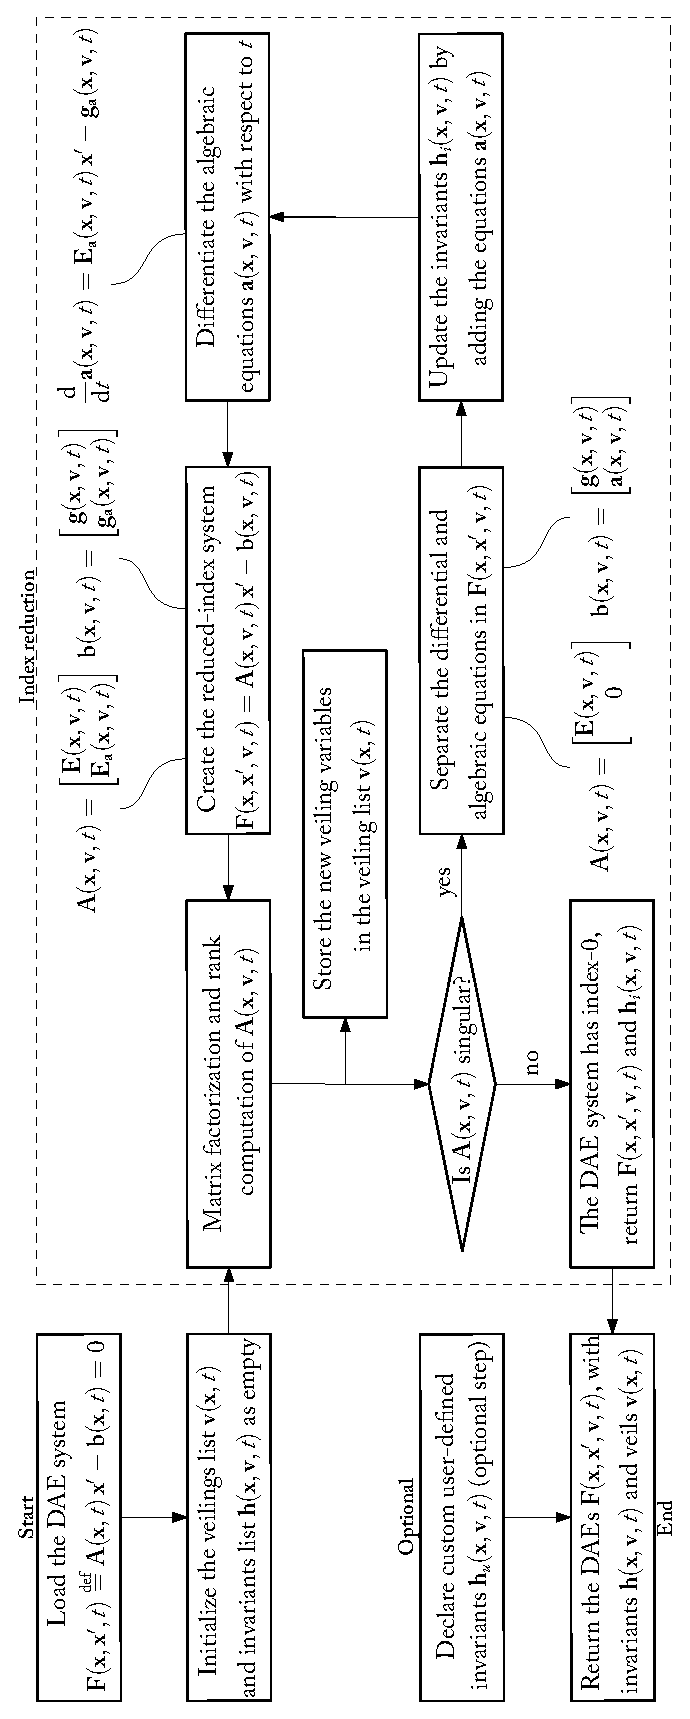
\includegraphics[angle=270, width=\textwidth]{dae_flowchart_veil}
  \caption{Flowchart of the index reduction algorithm with expression swell mitigation.}
  \label{chap4:fig:index_reduction_veil}
\end{sidewaysfigure}

% % % % % % % % % % % % % % % % % % % % % % % % % % % % % % % % % % % % % % % %

\section{The Symbolic-Numeric Solution Scheme}
\label{chap4:sec:indigo}

After this fairly long discussion on the actual implementation aspects of the index reduction algorithm, we can now present the \Indigo{} index reduction and integration toolbox~\cite{indigo}. This toolbox consists of two main components: a \Maple{} package to carry out symbolic index reduction of \ac{DAE} systems, and a \Matlab{} toolbox to perform numerical integration of the reduced-index system. \Indigo{} is designed to be used in conjunction with the \LEM{} package, to limit the expression swell, and the \LAST{} package, to conveniently factorize matrices. In the following paragraphs, we briefly discuss the usage of the \Indigo{} package.

\subsection{Index Reduction}

The index reduction algorithm implemented in the \Indigo{} \Maple{} package is the one presented in Section~\ref{chap4:sec:algorithm}. To reduce the index of a \ac{DAE} system in the \Maple{} environment we need to first create an \Indigo{} object instance.
%
\begin{verbatim}
> Indigo_obj := Object(Indigo);
> Indigo_obj:-InitLAST();
\end{verbatim}
%
Then, the system of \acp{DAE} \texttt{eqns} with coordinates \texttt{vars} is loaded.
%
\begin{verbatim}
> Indigo_obj:-LoadEquations('Generic', eqns, vars);
\end{verbatim}
%
The \texttt{Generic} symbol is used to specify the type of the system. Notice that in this example, we assume that the equations of the system are already available in the \Maple{} session. The automatic index reduction process can be performed by calling the \texttt{ReduceIndex} method, which iterates the separation and differentiation steps until an index-$0$ \ac{DAE} system is obtained.
%
\begin{verbatim}
> Indigo_obj:-ReduceIndex();
\end{verbatim}
%
Intermediate results of the process are stored internally in the \Indigo{} object and are available on demand. Once the index reduction process is completed, the user can generate the \texttt{name} \Matlab{} class file to perform numerical integration of the reduced-index system.
%
\begin{verbatim}
> Indigo_obj:-GenerateMatlabCode(name, type, data=pars);
\end{verbatim}
%
A file \texttt{name.m} is generated in the current directory. As it is explained in the next section, The string parameter \texttt{type} can be either \texttt{Implicit}, \texttt{SemiExplicit} or \texttt{Explicit} depending on the desired numerical integration scheme. The optional parameter \texttt{data} introduces default internal object data.

\subsection{Numerical Integration Scheme}

The \Indigo{} \Matlab{} toolbox is an object-oriented library that allows the user to exploit the automatically generated code of the reduced-index system. It is capable of integrating systems of \acp{ODE} and \acp{DAE} using a variety of \ac{RK} numerical integration schemes. In particular, the system of equations which is integrated is composed of the following elements.
%
\begin{itemize}
  \setlength{\itemsep}{0.0em}
  \item A differential part, which can be expressed by one of the following classes:
  %
  \begin{equation*}
      \begin{array}{ccl}
          \m{F}(\mx, \mx^\prime, \m{v}, t) = \m{0} & \hspace{0.5cm} &
          \text{\texttt{Implicit} system class,} \\[0.5mm]
          \m{A}(\mx, \m{v}, t) \, \mx^\prime = \m{b}(\mx, \m{v}, t) & \hspace{0.5cm} &
          \text{\texttt{SemiExplicit} system class,} \\[0.5mm]
          \mx^\prime = \m{f}(\mx, \m{v}, t) & \hspace{0.5cm} &
          \text{\texttt{Explicit} system class.}
      \end{array}
  \end{equation*}
  %
  \item The invariants, composed of the hidden constraints obtained from the index reduction process $\mhiv$, and optional user-defined invariants $\mhuv$, namely
  %
  \begin{equation*}
    \m{h}(\mx, \m{v}, t) = \begin{bmatrix}
        \mhiv \\[0.5mm]
        \mhuv
    \end{bmatrix} = \m{0} \, \text{.}
  \end{equation*}
  %
  \item The veils, which are the set of the expression hierarchical representation variables used in \LEM{} to limit the expression swell
  %
  \begin{equation*}
      \m{v}(\mx, t) = \begin{bmatrix}
          v_{1}(\mx, t) \\[0.5mm]
          v_{2}(v_{1}, \mx, t) \\
          \vdots \\
          v_{n}(v_{1}, \dots, v_{n-1}, \mx, t)
      \end{bmatrix} \, \text{.}
  \end{equation*}
\end{itemize}

To respect the invariants during the integration the \emph{standard projection} method is applied~\cite{hairer2000symmetric}. This method consists of projecting the solution $\mx$ of the numerically integrated reduced-index system onto the invariants manifold $\m{h}(\mx, \m{v}, t) = \m{0}$, which is equivalent to the following constrained minimization
%
\begin{equation*}
  \underset{\widetilde{\mx}}{\textrm{minimize}} \quad \dfrac{1}{2}\left(\mx - \widetilde{\mx}\right)^2
    \quad \textrm{subject to} \quad
    \m{h}(\mx, \m{v}, t) = \m{0}.
\end{equation*}

To integrate the system generated through the \Matlab{} package or a custom system \texttt{sys}, the user must first instantiate a \Indigo{} \ac{RK} solver.
%
\begin{verbatim}
>>> solver = IndigoSolver('solver_name');
>>> solver.set_system(sys);
\end{verbatim}
%
Once the solver is instantiated, it is only necessary to specify the \acp{IC} and the integration time vector.
%
\begin{verbatim}
>>> [x, t, v, h] = solver.solve(t_ini:d_t:t_end, ics);
\end{verbatim}
%
The solver returns the solution of the system in the form of multiple outputs: \texttt{x} contains the integrated solution, \texttt{x\_dot} the states' time derivative, \texttt{t} the time vector, \texttt{v} the veiling variables, and finally \texttt{h} the values of the invariants over the specified time mesh \texttt{t\_ini:d\_t:t\_end}.

\subsection{Proving the Algorithm Implementation}
\label{chap4:sec:example}

In this section, we showcase an example of a high-index \ac{DAE} system: an index-3 problem with an analytical solution, which describes the motion of a particle on a 3D torus surface~\cite{campbell1995constraint}. This example is employed to validate the numerical stability of the reduced-index system, as well as the good conditioning of both the symbolic matrix factorization and the numerical integration scheme. To ease the understanding of the results, we purposely avoid the use of the veiling variables in this example. However, the veiling variables just add an evaluation layer to the expressions, and they do not affect the numerical properties of the integrator.

\subsubsection{Expression Complexity of the Reduced-Index Systems}
\label{chap4:sec:daes_complexity}

As a first demonstration of the proposed index reduction algorithm capabilities, we first consider the given example from a purely symbolic perspective. In particular, we consider the computational cost of the expressions generated during the presented procedure, both with \ac{LU} and \ac{FFLU} factorization of the system matrix. The compactness of the expressions generated during the index reduction algorithm is a crucial aspect, as it ensures that limited computational overhead is introduced in the numerical integration of the reduced-index system, as well as in the projection of the solution on the hidden constraints. Specifically, the index reduction algorithm is applied to the \ac{DAE} system and reduced to index-0. For each reduction stage of the example considered, the computational cost is reported in Table~\ref{chap4:tab:torus}. Notably, the results show that the expression complexity is similar for both \ac{LU} and \ac{FFLU} factorization, with a slight increase in the number of multiplications and divisions for the latter.

\begin{table}[htb]
  \caption{Expression complexity encountered throughout the index reduction of the particle motion \ac{DAE} system with both the \ac{LU} and \ac{FFLU} factorization techniques. \emph{Legend}: $\cf$ = functions, $\ca$ = additions, $\cm$ = multiplications, and $\cd$ = divisions.}
  \label{chap4:tab:torus}
  \centering
  {\small\begin{tabular}{cccc}
    \multicolumn{4}{c}{\textbf{Particle Motion} (LU Factorization)~\cite{campbell1995constraint}} \\
    \toprule
    \textbf{Original \acp{DAE}} & \multicolumn{3}{c}{$\mF = 47\cf + 30\cm + 23\ca$ \quad $\mh = 0$} \\
    \midrule
    \textbf{Reduction step} & $\mE$ & $\mg$ & $\ma$ \\
    \midrule
    Index-3 \acp{DAE} & $0$ & $39\cf + 36\cm + 13\ca$ & $7\cf + 10\cm + 6\ca$ \\
    Index-2 \acp{DAE} & $0$ & $39\cf + 36\cm + 13\ca$ & $22\cf + 20\cm + 8\ca$ \\
    Index-1 \acp{DAE} & $0$ & $39\cf + 36\cm + 13\ca$ & $68\cf + 72\cm + 33\ca$ \\
    Index-0 \acp{DAE} & $388\cf + 424\cm + 180\ca$ & $79\cf + 77\cm + 26\ca$ & $0$ \\
    \midrule
    \textbf{Reduced \acp{DAE}} & \multicolumn{3}{c}{$\mF = 258\cf + 239\cm + 109\ca$ \quad $\mh = 97\cf + 102\cm + 47\ca$} \\
    \bottomrule \\[0.5em]
    %
    \multicolumn{4}{c}{\textbf{Particle Motion} (FFLU Factorization)~\cite{campbell1995constraint}} \\
    \toprule
    \textbf{Original \acp{DAE}} & \multicolumn{3}{c}{$\mF = 47\cf + 30\cm + 23\ca$ \quad $\mh = 0$} \\
    \midrule
    \textbf{Reduction step} & $\mE$ & $\mg$ & $\ma$ \\
    \midrule
    Index-3 \acp{DAE} & $0$ & $39\cf + 36\cm + 13\ca$ & $7\cf + 10\cm + 6\ca$ \\
    Index-2 \acp{DAE} & $0$ & $39\cf + 36\cm + 13\ca$ & $26\cf + 23\cm + 8\ca$ \\
    Index-1 \acp{DAE} & $0$ & $39\cf + 36\cm + 13\ca$ & $68\cf + 72\cm + 33\ca$ \\
    Index-0 \acp{DAE} & $388\cf + 424\cm + 180\ca$ & $79\cf + 77\cm + 26\ca$ & $0$ \\
    \midrule
    \textbf{Reduced \acp{DAE}} & \multicolumn{3}{c}{$\mF = 258\cf + 239\cm + 109\ca$ \quad $\mh = 97\cf + 105\cm + 47\ca$} \\
    \bottomrule
    \end{tabular}}
\end{table}

\subsubsection{Numerical Integration of the Reduced-Index System}
\label{chap4:sec:numerical_integration}

The numerical stability and consistency of the reduced-index system are demonstrated by exploiting the analytical solution of the problem in~\cite{campbell1995constraint}. Specifically, the \ac{DAE} system consists of three position variables $[x_{1}, \, x_{2}, \, x_{3}]^\top$, three velocity variables $[u_{1}, \, u_{2}, \, u_{3}]^\top$, and one constraint with Lagrange multiplier $\lambda$. The solution manifold is 4D, and the exact solution is
%
\begin{equation*}
  \mx_\text{exact} = \begin{bmatrix}
    x_{1} \\ x_{2} \\ x_{3}
  \end{bmatrix} = \begin{bmatrix}
    (\rho \cos(2\pi - t) + r) \cos(t) \\
    (\rho \cos(2\pi - t) + r) \sin(t) \\
    \rho \sin(2\pi - t)
  \end{bmatrix} \, \text{.}
\end{equation*}
%
The initial value problem is defined as follows
%
\begin{equation}
  \label{chap4:eq:torus}
  \mF = \begin{bmatrix}
    x^{\prime}_{1} - u_{1} \\
    x^{\prime}_{2} - u_{2} \\
    x^{\prime}_{3} - u_{3} \\
    u^{\prime}_{1} - u_{3}\cos(t) + x_{3}\sin(t) + u_{2} - 2 c x_{1}\lambda \\
    u^{\prime}_{2} - u_{3}\sin(t) - x_{3}\cos(t) - u_{1} - 2 c x_{2}\lambda \\
    u^{\prime}_{3} + x_{3} - 2x_{3}\lambda \\
    x_{1}^2 + x_{2}^2 + x_{3}^2 - 2r(x_{1}^2 + x_{2}^2)^{1/2} + r^2 - \rho^2
  \end{bmatrix} \, \text{,}
\end{equation}
%
with parameters $\rho = 5$ and $r = 10$, $c = 1 - {r} / {(x_{1}^2 + x_{2}^2)^{1/2}}$, states $\mx = [x_{1}, \, x_{2}, \, x_{3}, \, u_{1},$ $u_{2}, \, u_{3}, \, \lambda]^{\top}$, and \acp{IC} $\mx_{0} = [15, \, 0, \, 0, \, 0, \, 15, \, -5, \, \lambda]^{\top}$.

The numerical integration of the reduced-index system is performed through Implicit Euler, RadauIIA3, and RadauIIA5 \ac{RK} methods. To respect the invariants during the integration the \emph{standard projection} method is applied~\cite{hairer2000symmetric}. This method consists of projecting the solution $\mx$ of the numerically integrated system onto the invariants on the hidden constraints $\mh = \m{0}$, which is equivalent to the constrained minimization
%
\begin{equation*}
  \underset{\tilde{\mx}}{\textrm{minimize}} \quad \dfrac{1}{2}\left(\mx - \tilde{\mx}\right)^2
    \quad \textrm{subject to} \quad
    \mh = \m{0} \, \text{.}
\end{equation*}
%
To verify that the projection is performed correctly and does not affect the order of the \ac{RK} method, numerical integration is performed in the interval $t \in [0, \, 2\pi]$ seconds with different integration time steps $\Delta t$. The error of the numerical integration $\varepsilon = \| \mx - \mx_\text{exact} \|_{\infty}$ is reported in \figurename~\ref{chap4:fig:torus_order}. As it can be seen, the implemented projection preserves the order of the method for all the integration time steps. It is important to highlight that to obtain such results the absolute error tolerances of the integrator and the projection are both set to $\varepsilon = 10^{-10}$. The same tolerances are used in the numerical integration of the reduced-index system in the interval $t \in [0, \, 400\pi]$ seconds with step $\Delta t = 0.025$ seconds. The results are reported in \figurename~\ref{chap4:fig:torus_integration}, where Implicit Euler, RadauIIA3, and RadauIIA5 \ac{RK} methods are employed, and the projection on the hidden constraints $\mh$ is performed. The effect of the projection is highlighted on the bottom left plot.

\begin{figure}[htb]
  \centering
  \small{\includetikz{figures/chapter_4/torus_order_hidden.tex}}
  \caption{Numerical integration error $\varepsilon = \| \mx - \mx_\text{exact} \|_{\infty}$ of the \acp{DAE}~\eqref{chap4:eq:torus} over different integration time steps $\Delta t$, along with the computed order of the method (left). The projection on the hidden constraints is performed and the invariants violation $\| \mh \|_{\infty}$ is reported (right). Notice that the implemented projection preserves the order of the method for all the integration time steps. The tests are performed in $t \in [0, \, 2\pi]$ seconds, using Implicit Euler, RadauIIA3, and RadauIIA5 \ac{RK} methods.}
  \label{chap4:fig:torus_order}
\end{figure}

\begin{figure}[htbp]
  \centering
  \small{\includetikz{figures/chapter_4/torus_implicit_euler.tex}}%
  \hspace{0.25cm}%
  \small{\includetikz{figures/chapter_4/torus_radauiia3.tex}}
  \small{\includetikz{figures/chapter_4/torus_radauiia5.tex}}%
  \hspace{0.25cm}%
  \small{\includetikz{figures/chapter_4/torus_radauiia5_noproj.tex}}
  \caption{Numerically integrated solution of the \acp{DAE}~\eqref{chap4:eq:torus} in the interval $t \in [0, \, 400\pi]$ seconds, with step $\Delta t = 0.025$ seconds, using Implicit Euler (top left), RadauIIA3 (top right), and RadauIIA5 (bottom left and right) \ac{RK} methods.}
  %The first three plots show the numerical integration of the reduced-index system with projection on the hidden constraints $\mh$ produced by the index reduction algorithm. On the bottom right plot, the numerical integration of the reduced-index system is performed without projection on the manifold $\mh$ and substantial drift is observed.}
  \label{chap4:fig:torus_integration}
\end{figure}

% % % % % % % % % % % % % % % % % % % % % % % % % % % % % % % % % % % % % % % %
%!TEX root = ../main.tex

\chapter{Application Fields and Examples}
\label{chap5:applications}

In the previous chapter, we presented a methodology for the automatic index reduction of \ac{DAE} systems. The index reduction algorithm is based on the separation of the system into differential and algebraic parts with the help of symbolic linear algebra, \ie{}, \ac{LU} or \ac{FFLU} matrix factorization. No information on the \ac{DAE} system structure is leveraged during the reduction algorithm and, for this reason, this methodology can be applied to generic \acp{DAE} linear in the state derivatives. Numerical integration goodness is showcased by assessing the order of the numerical integration scheme and the accuracy of the projection. In this chapter, we take for granted the correctness of the proposed methodology and we focus on the application and capabilities of the index reduction algorithm. Hence, the algorithm is applied to a variety of \ac{DAE} systems, which are specifically chosen to demonstrate the capabilities, the potential, as well as the wide range of applicability of the proposed methodology. The examples are divided into three main categories: \emph{multibody dynamics}, \emph{trajectory prescribed path control}, and \emph{electrical networks}. Each of these categories is characterized by a different structure of the \ac{DAE} system, which will be analyzed in detail and will help us to understand the effectiveness of the proposed methodology. The examples are mainly taken from the testsets~\cite{lioen1998test, mazzia2003test, mazzia2008test, mazzia2012test} and are the following.
%
\begin{enumerate}
  \setlength\itemsep{0.0em}
  \item Multibody dynamics field:
  \begin{enumerate}
    \setlength\itemsep{0.0em}
    \item car-axis system~\cite{lioen1998test, mazzia2008test};
    \item flexible slider-crank mechanism~\cite{lioen1998test, mazzia2008test};
    \item the multi-pendula system~\cite{nedialkov2008solvingIII};
    \item double-wishbone suspension system~\cite{lioen1998test, mazzia2008test}.
  \end{enumerate}
  \item Trajectory prescribed path control applications:
  \begin{enumerate}
    \setlength\itemsep{0.0em}
    \item initial stage space shuttle reentry problem~\cite{brenan1995numerical};
    \item final stage space shuttle reentry problem~\cite{brenan1995numerical};
    \item the robotic arm system~\cite{pryce1998solving}.
  \end{enumerate}
  \item Electrical networks field:
  \begin{enumerate}
    \setlength\itemsep{0.0em}
    \item eight-nodes transistor-amplifier~\cite{lioen1998test, mazzia2008test};
    \item electric ring modulator~\cite{lioen1998test, mazzia2008test};
    \item cascaded differential amplifier~\cite{brenan1995numerical}.
  \end{enumerate}
\end{enumerate}

A comparison between the built-in joint index reduction algorithm and numerical integration schemes offered by \Maple{} with those of \Indigo{} will demonstrate the effectiveness of the proposed methodology and software implementation. It must be pointed out that, to ensure a fair comparison, the same numerical integration method is used in both software packages, \ie{}, the \ac{RKF} 4(5) method with a relative tolerance of $10^{-6}$ and an absolute tolerance of $10^{-7}$. Only when it is not possible to integrate the system with the chosen method, the integration is performed with the RadauIIA5 method in \Indigo{} and the implicit Rosenbrock 3(4) method in \Maple{}. The computation time limit is set to \SI{100}{\second} for both index reduction and code generation. Numerical integration is not limited by time, but the results are reported only if the integration is thoroughly completed.

For the sake of completeness, we also compare \emph{some} of our results with those obtained by the \Matlab{} symbolic toolbox, which works under a \MuPAD{} \ac{CAS}. Notably, \Matlab{} is capable of performing \acp{DAE} index reduction through either the Pantelides algorithm (\texttt{reduceDAEToODE} function)~\cite{pantelides1988consistent} or the Gaussian elimination method (\texttt{reduceDAEIndex} function). The latter is claimed to be more robust and, to some extent, might be similar to the approach proposed in this work, although its working principles are not fully disclosed and its success is guaranteed only if semilinear \ac{DAE} systems are considered. However, the Pantelides algorithm is reported to be less robust and to have a higher computational cost~\cite{matlabdaes}. For the same examples, we also include the results obtained by the \Mathematica{} symbolic toolbox, which is capable of performing \acp{DAE} index reduction through the Pantelides algorithm as well. It is worth noticing that \Mathematica{} does not provide access to the reduced index \ac{DAE} system, moreover, \Matlab{} has no built-in function to compute the computational cost of each equation in the reduced-index \ac{DAE} system. This makes the comparison with the proposed methodology and software package more challenging. For this reason, we will only limit our considerations to overall performance, \ie{}, the success of both index reduction process and numerical integration processes. A summary of this comparison will be later reported in Table~\eqref{chap5:tab:numerical_integration}.

But before we proceed with the examples, it is also worth mentioning that during the index reduction process, the trigonometric identities provided by Weierstra{\ss}~\eqref{chap3:eq:weierstrass} or~\eqref{chap3:eq:zhou} can be used to slightly reformulate the \acp{DAE}expressions, as well as to obtain polynomials expressions and improve the detection of symbolic eliminations (see Section~\ref{chap3:sec:signature}). However, the use of such trigonometric identities does not typically lead to a significant improvement in the computational cost of the expressions generated during the index reduction procedure as the polynomial expressions obtained are hard to simplify as well. Furthermore, such transformations impose a change of coordinates in the original \ac{DAE} system, which may be undesirable in some applications. For this reason, no reformulation is performed in the examples presented in this chapter.

\section{Multibody Dynamics}
\label{chap5:sec:mbd}

Historically, the \ac{MBD} problems appeared in the early 60s when the first computer simulations of mechanical systems were performed. Over the years, such systems have been studied extensively, and many numerical or hybrid symbolic-numeric methods have been developed to solve them. As a consequence, the \ac{MBD} field has become one of the most important areas of research in the mechanical engineering domain having a wide range of applications. In this section, we present four examples of \ac{MBD} problems, which are solved using the proposed index reduction algorithm. But first, we provide a brief overview of the \ac{MBD} problems, their mathematical formulation, as well as the formal index reduction of the corresponding generic \ac{MB} \acp{DAE}.

The \ac{MBD} category is characterized by \ac{DAE} systems that describe the motion of a mechanism composed of interconnected rigid or flexible bodies. Within these systems, the differential equations represent motion equations, while the algebraic equations correspond to kinematic constraints, collectively constituting these \ac{MB} problems. Typically, such problems are posed as Hessenberg semi-explicit index-3 \acp{DAE} of the form
%
\begin{equation}
  \begin{cases}
    \m{p} = \m{q}^{\prime} \\
    \m{M}(\m{q}, \m{p}, t)\m{p}^{\prime} - \jac{\bm{\Phi}}{\m{q}}(\m{q}, t)^{\top}\bm{\lambda} = \m{f}(\m{q}, \m{p} ,t) \\
    \bm{\Phi}(\m{q}, t) = \m{0}
  \end{cases} \, \text{,}
  \qquad \text{with} \qquad \jac{\bm{\Phi}}{\m{q}}(\m{q}, t) = \dfrac{\partial}{\partial\m{q}}\bm{\Phi}(\m{q}, t)
  \, \text{,}
  \label{chap5:eq:mbd_fo}
\end{equation}
%
where $\m{q} \in \mathbb{R}^{n}$ and $\m{p} \in \mathbb{R}^{n}$ indicate respectively the generalized coordinates and the generalized velocities, $\m{M}(\m{q}, \m{p}, t) \in \mathbb{R}^{n\times n}$ is the mass matrix, $\bm{\Phi}(\m{q}, t) \in \mathbb{R}^{m}$ is the constraint vector, $\bm{\lambda} \in \mathbb{R}^{m}$ is the vector of Lagrange multipliers, and lastly $\m{f}(\m{q}, \m{p}, t) \in \mathbb{R}^{n}$ collects all the contributions from Coriolis and centrifugal effects, as well as external forces.

\paragraph{Index Reduction of Multibody Dynamics Equations}

To solve the problem in~\eqref{chap5:eq:mbd_fo}, one of the possible approaches is to transform the problem into a system of \acp{ODE} with invariants. Moreover, one may also isolate the Lagrange multipliers $\bm{\lambda}$ and write them explicitly in terms of the state variables so as to obtain an index-1 \acp{DAE} representation of the \ac{MBD} problem. In such cases, the index reduction can be performed by exploiting the structure of the problem, as well as the properties of the mass matrix $\m{M}(\m{q}, \m{p}, t)$ and constraint vector $\bm{\Phi}(\m{q}, t)$. To do so, we first need to differentiate the constraint $\bm{\Phi}(\m{q}, t)$, this yields to
%
\begin{equation}
  \dfrac{\de{}}{\de{} t}\bm{\Phi}(\m{q}, t) = \jac{\bm{\Phi}}{\m{q}}(\m{q}, t) + \jac{\bm{\Phi}}{t}(\m{q}, t) = \m{0}
  \, \text{,}
  \qquad \text{with} \qquad \jac{\bm{\Phi}}{t}(\m{q}, t) = \dfrac{\partial}{\partial t}\bm{\Phi}(\m{q}, t)
  \, \text{.}
  \label{chap5:eq:mbd_hidden_1}
\end{equation}
%
Notice that when constraint does not depend on time~\eqref{chap5:eq:mbd_hidden_1} expresses the intuitive idea that generalized velocity $\m{p}$ must be orthogonal to constraint's gradient. This provides also the opportunity to highlight that constraint $\bm{\Phi}(\m{q}, t)$ imposes relationships also at the velocity and acceleration level, \ie{},~\eqref{chap5:eq:mbd_hidden_1} restricts the set of feasible velocities. Finally, it must be noticed that~\eqref{chap5:eq:mbd_hidden_1} is still algebraic in the $\m{p}$ coordinates, thus in order to obtain a fully differential relationship, another differentiation is needed. This results in the following equation
%
\begin{equation}
  \dfrac{\de{}^2}{\de{}t^2}\bm{\Phi}(\m{q}, t) = \hes{\bm{\Phi}}{\m{q}t}(\m{q}, t)\m{p} + \jac{\bm{\Phi}}{\m{q}}(\m{q}, t)\m{p}^{\prime} + \dif{\bm{\Phi}}{tt}(\m{q}, t) = \m{0} \, \text{,}
  \label{chap5:eq:mbd_hidden_2}
\end{equation}
\begin{equation*}
  \text{with} \qquad
  \dif{\bm{\Phi}}{tt}(\m{q}, t) = \dfrac{\partial^2}{\partial t^2}\bm{\Phi}(\m{q}, t) \, \text{,}
  \qquad \text{and} \qquad
  \hes{\bm{\Phi}}{\m{q}t}(\m{q}, t) = \dfrac{\de{}}{\de{} t}\,\jac{\bm{\Phi}}{\m{q}}(\m{q}, t) \, \text{,}
\end{equation*}
%
which does not impose any algebraic constraint on the mechanical system states and leads to the following index-1 \ac{DAE} system
%
\begin{equation}
  \begin{cases}
    \m{q}^{\prime} = \m{p} \\
    \m{M}(\m{q}, \m{p}, t)\m{p}^{\prime} - \jac{\bm{\Phi}}{\m{q}}(\m{q}, t)^{\top}\bm{\lambda} = \m{f}(\m{q},\m{p},t) \\
    -\jac{\bm{\Phi}}{\m{q}}(\m{q}, t)\m{p}^{\prime} = \hes{\bm{\Phi}}{\m{q}t}(\m{q}, t)\m{p} + \dif{\bm{\Phi}}{tt}(\m{q}, t)
  \end{cases} \, \text{.}
  \label{chap5:eq:mbd_ode}
\end{equation}
%
System~\eqref{chap5:eq:mbd_ode} can be also written in compact matrix notation as
%
\begin{equation}
  \label{chap5:eq:mbd_ode_matrix}
  \begin{bmatrix}
    \m{I} & \m{0} & \m{0} \\
    \m{0}      & \m{M}(\m{q}, \m{p}, t) & -\jac{\bm{\Phi}}{\m{q}}(\m{q}, t)^{\top} \\
    \m{0}      & -\jac{\bm{\Phi}}{\m{q}}(\m{q}, t) & \m{0}
  \end{bmatrix}
  \begin{bmatrix}
    \m{q}^{\prime} \\
    \m{p}^{\prime} \\
    \bm{\lambda}
  \end{bmatrix}
  =
  \begin{bmatrix}
    \m{p} \\
    \m{f}(\m{q},\m{p},t) \\
    \hes{\bm{\Phi}}{\m{q}t}(\m{q}, t)\m{p} + \dif{\bm{\Phi}}{tt}(\m{q}, t)
  \end{bmatrix} \, \text{.}
\end{equation}
%
It is easy to notice that if the left-hand side matrix of~\eqref{chap5:eq:mbd_ode_matrix} is invertible, then we can write the system in explicit form. In specific, the matrix is invertible if and only if the sub-block
%
\begin{equation*}
  \begin{bmatrix}
    \m{M}(\m{q}, \m{p}, t) & -\jac{\bm{\Phi}}{\m{q}}(\m{q}, t)^{\top} \\
    -\jac{\bm{\Phi}}{\m{q}}(\m{q}, t) & \m{0}
  \end{bmatrix}
  \in\mathbb{R}^{(n+m)\times(n+m)}
\end{equation*}
%
is non-singular. To prove its non-singularity the rank additivity formula is applied as follows
%
\begin{equation*}
  \mathrm{rank}\left(
  \begin{bmatrix}
    \m{M}(\m{q}, \m{p}, t) & -\jac{\bm{\Phi}}{\m{q}}(\m{q}, t)^{\top} \\
    -\jac{\bm{\Phi}}{\m{q}}(\m{q}, t) & \m{0}
  \end{bmatrix}\right)
  = \mathrm{rank}\left(\m{M}(\m{q}, \m{p}, t)\right) + \mathrm{rank}\left( \jac{\bm{\Phi}}{\m{q}}(\m{q}, t)\m{M}(\m{q}, \m{p}, t)^{-1} \jac{\bm{\Phi}}{\m{q}}(\m{q}, t)^{\top}\right) \, \text{.}
\end{equation*}
%
Since $\m{M}(\m{q}, \m{p}, t)$ is positive definite (and thus also non-singular), then $\forall\m{q} \in \mathbb{R}^{n}, \mathrm{rank}({\m{M}(\m{q}, \m{p}, t)}) = n$. Moreover, the second term in the right-hand side of the equation above is non-negative and it is zero if and only if
%
\begin{equation}
  \mathrm{rank}\left( \jac{\bm{\Phi}}{\m{q}}(\m{q}, t) \m{M}(\m{q}, \m{p}, t)^{-1} \jac{\bm{\Phi}}{\m{q}}(\m{q}, t)^{\top}\right) = m \, \text{,}
  \label{chap5:eq:compression}
\end{equation}
%
which is not generally true. However, if we assume that the constraints are \emph{locally} linearly independent, then $\forall\m{q}\in\mathbb{R}^{n},\forall t$, the rank of the Jacobian matrix $\jac{\bm{\Phi}}{\m{q}}(\m{q}, t) = m$. Therefore, the matrix in~\eqref{chap5:eq:mbd_ode_matrix} is invertible and the overall system can be written explicitly as
%
\begin{equation*}
  \begin{bmatrix}
    \m{q}^{\prime} \\ \m{p}^{\prime} \\ \bm{\lambda}
  \end{bmatrix} = \begin{bmatrix}
    \m{I} & \m{0} & \m{0} \\
    \m{0} & \m{M}(\m{q}, \m{p}, t) & -\jac{\bm{\Phi}}{\m{q}}(\m{q}, t)^{\top} \\
    \m{0} & -\jac{\bm{\Phi}}{\m{q}}(\m{q}, t) & \m{0}
  \end{bmatrix}^{-1}
  \begin{bmatrix}
    \m{p} \\
    \m{f}(\m{q},\m{p},t) \\
    \hes{\bm{\Phi}}{\m{q}t}(\m{q}, t)\m{p} + \dif{\bm{\Phi}}{tt}(\m{q}, t)
  \end{bmatrix}
\end{equation*}
%
An explicit expression for the inverse matrix above can be obtained through tedious symbolic calculations. However, regardless of the specific solution, we want to stress a very important point: by differentiating the constraint twice we are now able to explicitly write an expression for the Lagrange multipliers (index-1 variables). If the accelerations $\m{p}^{\prime}$ are isolated from~\eqref{chap5:eq:mbd_ode_matrix} and substituted into~\eqref{chap5:eq:mbd_hidden_2}, we obtain
%
\begin{equation}
  \m{p}^{\prime} = \m{M}(\m{q}, \m{q}^{\prime}, t)^{-1} \jac{\bm{\Phi}}{\m{q}}(\m{q}, t)^{\top}\bm{\lambda} + \m{M}(\m{q}, \m{q}^{\prime}, t)^{-1}\m{f}(\m{q},\m{p},t) = \m{0} \, \text{.}
  \label{chap5:eq:gen_vel}
\end{equation}
%
Then, substituting~\eqref{chap5:eq:gen_vel} into~\eqref{chap5:eq:mbd_hidden_2} we obtain the following expression
%
\begin{equation}
  \hes{\bm{\Phi}}{\m{q}t}(\m{q}, t)\m{p} + \jac{\bm{\Phi}}{\m{q}}(\m{q}, t)\m{M}(\m{q}, \m{q}^{\prime}, t)^{-1} \jac{\bm{\Phi}}{\m{q}}(\m{q}, t)^{\top}\bm{\lambda} + \jac{\bm{\Phi}}{\m{q}}(\m{q}, t)\m{M}(\m{q}, \m{q}^{\prime}, t)^{-1} \m{f}(\m{q},\m{p},t)+\dif{\bm{\Phi}}{tt}(\m{q}, t) = 0 \, \text{.}
\end{equation}
%
Here the non-singular matrix in~\eqref{chap5:eq:compression} can be easily recognized, therefore the expression for the Lagrange multipliers is given by
%
\begin{equation*}
  \bm{\lambda} = -\left(\jac{\bm{\Phi}}{\m{q}}(\m{q}, t)\m{M}(\m{q}, \m{q}^{\prime}, t)^{-1} \jac{\bm{\Phi}}{\m{q}}(\m{q}, t)^{\top}\right)^{-1} \Big(\hes{\bm{\Phi}}{\m{q}t}(\m{q}, t)\m{p} + \jac{\bm{\Phi}}{\m{q}}(\m{q}, t)\m{M}(\m{q}, \m{q}^{\prime}, t)^{-1}\m{f}(\m{q},\m{p},t) + \dif{\bm{\Phi}}{tt}(\m{q}, t)\Big) \, \text{,}
\end{equation*}
%
which can be either substituted into the explicit form of the \ac{DAE} system~\eqref{chap5:eq:mbd_ode} or properly applied to obtain a numerically efficient representation of the \ac{MBD} problem, \ie{},
%
\begin{equation*}
  \text{a set of \acp{ODE}} \qquad
  \begin{cases}
    \m{q}^{\prime} = \m{p} \\
    \m{p}^{\prime} = \dot{\m{p}}
  \end{cases} \, \text{,} \\
\end{equation*}
%
where $\dot{\m{p}}$ is obtained by solving the linear system
%
\begin{equation*}
  \begin{bmatrix}
    \m{M}(\m{q}, \m{p}, t) & -\jac{\bm{\Phi}}{\m{q}}(\m{q}, t)^{\top} \\
    -\jac{\bm{\Phi}}{\m{q}}(\m{q}, t) & \m{0}
  \end{bmatrix}
  \begin{bmatrix}
    \dot{\m{p}} \\ \bm{\lambda}
  \end{bmatrix} = \begin{bmatrix}
    \m{f}(\m{q},\m{p},t) \\
    \hes{\bm{\Phi}}{\m{q}t}(\m{q}, t)\m{p} + \dif{\bm{\Phi}}{tt}(\m{q}, t)
  \end{bmatrix} \, \text{.}
\end{equation*}

Technically, mechanical systems subject to holonomic constraints are represented by \acp{DAE} systems of index 3, \ie{}, the differential index is one plus the number of differentiations of the constraint that are needed in order to be able to eliminate the Lagrange multipliers. Otherwise, equivalently, the number of times that we need to differentiate the constraint in order to obtain a differential equation also for each of the Lagrange multipliers.

\paragraph{Explicit Matrix Inverse}

For the sake of completeness, we provide the explicit expression for the inverse of matrix in~\eqref{chap5:eq:mbd_ode_matrix}, which is given by
%
\begin{equation*}
  \begin{bmatrix}
    \m{I} & \m{0} & \m{0} \\
    \m{0} & \m{M}(\m{q}, \m{p}, t) & -\jac{\bm{\Phi}}{\m{q}}(\m{q}, t)^{\top} \\
    \m{0} & -\jac{\bm{\Phi}}{\m{q}}(\m{q}, t) & \m{0}
  \end{bmatrix}^{-1}
  =
  \begin{bmatrix}
  \m{I} & \m{0} & \m{0} \\
  \m{0} & \m{X}_{11} & \m{X}_{12} \\
  \m{0} & \m{X}_{21} & \m{X}_{22}
  \end{bmatrix}
\end{equation*}
%
where the quantities $\m{X}_{11} \in \mathbb{R}^{n \times n}$, $\m{X}_{12} \in \mathbb{R}^{n \times m}$, $\m{X}_{21} \in \mathbb{R}^{m \times n}$, and $\m{X}_{22} \in \mathbb{R}^{m \times m}$ are defined as follows
%
\begin{equation*}
    \m{X}_{11} = \m{M}(\m{q}, \m{p}, t)^{-1} - \m{M}(\m{q}, \m{p}, t)^{-1} \jac{\bm{\Phi}}{\m{q}}(\m{q}, t)^{\top} \left(\jac{\bm{\Phi}}{\m{q}}(\m{q}, t) \m{M}(\m{q}, \m{p}, t)^{-1}\jac{\bm{\Phi}}{\m{q}}(\m{q}, t)^{\top}\right)^{-1} \jac{\bm{\Phi}}{\m{q}}(\m{q}, t)\m{M}(\m{q}, \m{p}, t)^{-1} \, \text{,}
\end{equation*}
\begin{equation*}
  \m{X}_{12} = -\m{M}(\m{q}, \m{p}, t)^{-1}\jac{\bm{\Phi}}{\m{q}}(\m{q}, t)^{\top} \left(\jac{\bm{\Phi}}{\m{q}}(\m{q}, t)\m{M}(\m{q}, \m{p}, t)^{-1} \jac{\bm{\Phi}}{\m{q}}(\m{q}, t)^{\top}\right)^{-1} \, \text{,}
\end{equation*}
\begin{equation*}
  \m{X}_{21} = -\left(\jac{\bm{\Phi}}{\m{q}}(\m{q}, t) \m{M}(\m{q}, \m{p}, t)^{-1}\jac{\bm{\Phi}}{\m{q}}(\m{q}, t)^{\top}\right)^{-1} \jac{\bm{\Phi}}{\m{q}}(\m{q}, t)\m{M}(\m{q}, \m{p}, t)^{-1} \, \text{,}
\end{equation*}
\begin{equation*}
  \m{X}_{22} = -\left(\jac{\bm{\Phi}}{\m{q}}(\m{q}, t) \m{M}(\m{q}, \m{p}, t)^{-1}\jac{\bm{\Phi}}{\m{q}}(\m{q}, t)^{\top}\right)^{-1} \, \text{.}
\end{equation*}
%
Notice that $\m{X}_{12} = \m{X}_{21}^{\top}$, as expected. Moreover, the matrix $\jac{\bm{\Phi}}{\m{q}}(\m{q}, t)\m{M}(\m{q}, \m{p}, t)^{-1} \jac{\bm{\Phi}}{\m{q}}(\m{q}, t)^{\top}$ also appears in~\eqref{chap5:eq:compression}, for which invertibility must be guaranteed.

\subsection{Car-Axis Dynamics}

After the introduction of the \ac{MBD} problems, we now present the first example, which is the car-axis dynamics problem. This example is taken from~\cite{lioen1998test, mazzia2008test} and is used to model the motion of a car as riding over an uneven road. Here, the system is modeled as two springs connected to two bars. The bottom of the left tire is the origin. The chassis is represented by a bar of mass $m$, and its position is given by $\m{q} = [x_l, y_l, x_r, y_r]^\top$, as also illustrated in Figure~\ref{chap5:fig:car_axis}. The left tire is always on a flat surface, while the right tire periodically rides over a sinusoidal road surface of height $y_b(t) = h\sin(\omega t)$. The distance between the wheels is fixed, and the car chassis must always have a fixed length, hence, the following constraints are imposed
%
\begin{equation*}
  \bm{\Phi}(\m{q}) = \begin{bmatrix}
    x_l x_b - y_l y_b \\
    (x_l - x_r)^2 + (y_l - y_r)^2 - \ell^2
  \end{bmatrix} = \m{0} \, \text{.}
\end{equation*}
%
The equations of motion for the car are derived using Lagrangian mechanics. The mass matrix $\m{M}$, and the force vector $\m{f}$ are given by
%
\begin{equation*}
  \m{M}(\m{q}) = \mathrm{diag}\left(
    (\ell_0-\ell_l)\dfrac{x_l}{\ell_l},
    (\ell_0-\ell_l)\dfrac{x_l}{\ell_l},
    (\ell_0-\ell_r)\dfrac{x_r}{\ell_r},
    (\ell_0-\ell_r)\dfrac{x_r}{\ell_r}
  \right)
  \quad \text{and} \quad
  \m{f} = \left[
    0, -\varepsilon^2\dfrac{m}{2},
    0, -\varepsilon^2\dfrac{m}{2}
  \right]^{\top}
  \, \text{,}
\end{equation*}
%
where
%
\begin{equation*}
  \ell_l = \sqrt{x_l^2 + y_l^2}
  \quad \text{and} \quad
  \ell_r = \sqrt{(x_r - x_b)^2 + (y_r - y_b)^2}
\end{equation*}
%
are respectively the length of the left and right springs, $\ell_0$ is the relaxed length of both springs, $h$ is the amplitude of the bump, and $1/\varepsilon^2$ is the Hooke's constant of the springs. The parameters of the car are chosen as $\ell = \SI{1}{\meter}$, $\ell_0 = \SI{1/2}{\meter}$, $\varepsilon = 0.01$, $m = \SI{10}{\kilo\gram}$, $h = \SI{0.1}{\meter}$, and $\omega = \SI{10}{\radian\per\second}$. While the \acp{IC} according to~\cite{lioen1998test, mazzia2008test} are $\m{q}_0 = [-1/2, 0, -1/2, 0]^\top$ and $\m{p}_0 = [0, 1/2, 1, 1/2]^\top$, with an integration time interval of $t \in \RSI{0}{3}{\second}$.

\begin{figure}
  \centering
  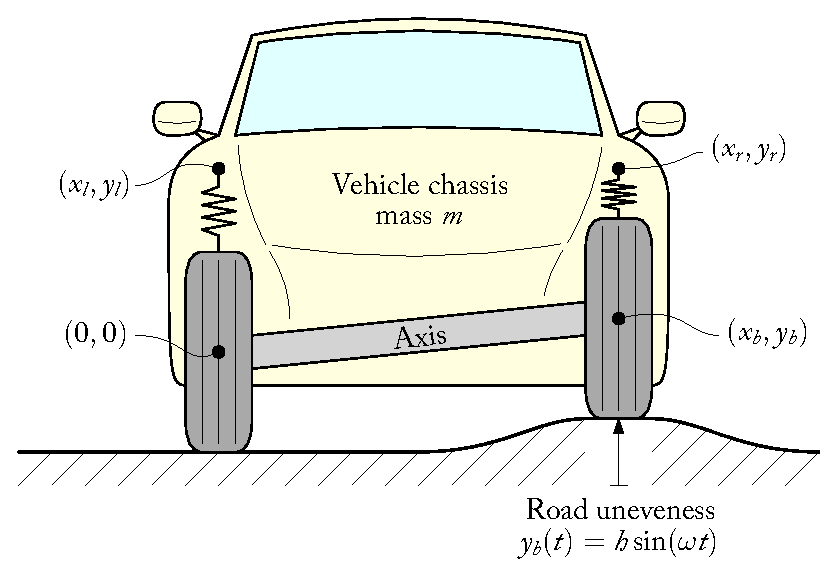
\includegraphics[width=0.7\textwidth]{figures/chapter_4/car_axis}
  \caption{Car-axis dynamics problem~\cite{lioen1998test, mazzia2008test}. The car is modeled as springs connected to two bars. The bottom of the left tire is the origin. The car chassis is represented by a bar of mass $m$. The position of the chassis is given by $\m{q} = [x_l, y_l, x_r, y_r]^\top$. The left tire is always on a flat surface, while the right tire periodically goes over a sinusoidal bump of the form $y_b(t) = h\sin(\omega t)$. The distance between the wheels must always remain fixed, and the car chassis must always have a fixed length.}
  \label{chap5:fig:car_axis}
\end{figure}

The car-axis \ac{DAE} system is solved using the proposed index reduction algorithm with both \ac{LU} and \ac{FFLU} factorization. The results are summarized in Table~\ref{chap5:tab:car_axis}. As expected, the index is reduced to 0, and the system is transformed into a set of \acp{ODE}. The complexity of the expressions encountered during the index reduction is given in terms of the number of functions $\cf$, additions $\ca$, multiplications $\cm$, and divisions $\cd$; and, as reported in the table, the index reduction is successful and little expression swell is observed only in the last reduction step. It should be noted that the \ac{FFLU} factorization produces more complex expressions than the \ac{LU} factorization and, for this reason, the former is dropped in the following simulations. The reduced system is then numerically solved using the \ac{RKF} 4(5) integrator, and the results are shown in Figure~\ref{chap5:fig:car_axis}, where the springs' lengths are plotted. Notably, during the simulation, the left spring remains nearly constant at its relaxed length, while the right spring periodically changes its length due to the bumps. It is worth mentioning that also \Mathematica{} and \Matlab{} (with both Pantelides and Gaussian elimination techniques) can correctly reduce the index of the car-axis problem and integrate the resulting system.

\begin{table}
  \caption{Expression complexity encountered throughout the index reduction of the car-axis problem~\cite{lioen1998test, mazzia2008test} \ac{DAE} system. \emph{Legend}: $\cf$ = functions, $\ca$ = additions, $\cm$ = multiplications, and $\cd$ = divisions.}
  \label{chap5:tab:car_axis}
  \centering
  {\footnotesize\begin{tabular}{cccc}
    \multicolumn{4}{c}{\textbf{Car-Axis (LU Factorization)~\cite{lioen1998test, mazzia2008test}}} \\
    \toprule
    \textbf{Original \acp{DAE}} & \multicolumn{3}{c}{$\mF = 108\cf + 131\cm + 56\ca$ \quad $\mh = 0$} \\
    \midrule
    \textbf{Reduction step} & $\mE$ & $\mg$ & $\ma$ \\
    \midrule
    Index-3 \acp{DAE} & $12\cm$ & $94\cf + 145\cm + 54\ca$ & $14\cf + 16\cm + 10\ca$ \\
    Index-2 \acp{DAE} & $12\cm$ & $94\cf + 145\cm + 54\ca$ & $26\cf + 45\cm + 15\ca$ \\
    Index-1 \acp{DAE} & $12\cm$ & $94\cf + 145\cm + 54\ca$ & $136\cf + 4\cd + 261\cm + 95\ca$ \\
    Index-0 \acp{DAE} & $1060\cf + 38\cd + 1901\cm + 717\ca$ & $431\cf + 8\cd + 842\cm + 268\ca$ & $0$ \\
    \midrule
    \textbf{Reduced \acp{DAE}} & \multicolumn{3}{c}{$\mF = 896\cf + 4\cd + 1202\cm + 546\ca$ \quad $\mh = 176\cf + 4\cd + 322\cm + 120\ca$} \\
    \bottomrule \\[0.5em]
    %
    \multicolumn{4}{c}{\textbf{Car-Axis (FFLU Factorization)~\cite{lioen1998test, mazzia2008test}}} \\
    \toprule
    \textbf{Original \acp{DAE}} & \multicolumn{3}{c}{$\mF = 108\cf + 131\cm + 56\ca$ \quad $\mh = 0$} \\
    \midrule
    \textbf{Reduction step} & $\mE$ & $\mg$ & $\ma$ \\
    \midrule
    Index-3 \acp{DAE} & $0$ & $94\cf + 8\cd + 150\cm + 54\ca$ & $14\cf + 21\cm + 10\ca$ \\
    Index-2 \acp{DAE} & $0$ & $94\cf + 8\cd + 154\cm + 54\ca$ & $26\cf + 1\cd + 44\cm + 15\ca$ \\
    Index-1 \acp{DAE} & $0$ & $94\cf + 8\cd + 155\cm + 54\ca$ & $136\cf + 6\cd + 4\cd + 261\cm + 95\ca$ \\
    Index-0 \acp{DAE} & $1066\cf + 55\cd + 1888\cm + 717\ca$ & $431\cf + 18\cd + 851\cm + 268\ca$ & $0$ \\
    \midrule
    \textbf{Reduced \acp{DAE}} & \multicolumn{3}{c}{$\mF = 1549\cf + 73\cd + 2765\cm + 1011\ca$ \quad $\mh = 176\cf + 7\cd + 326\cm + 120\ca$} \\
    \bottomrule
  \end{tabular}}
\end{table}

\begin{figure}[htb]
  \centering
  \small{\includetikz{figures/chapter_4/car_axis_length.tex}}
  \caption{Springs length of the car-axis problem~\cite{lioen1998test, mazzia2008test}. \emph{Legend}: \textcolor{mycolor1}{$\blacksquare$} left spring $L_l$, \textcolor{mycolor2}{$\blacksquare$} right spring $L_r$.}
  \label{chap5:fig:tppc_initial}
\end{figure}

\subsection{Flexible Slider-Crank Mechanism}

The slider-crank mechanism presented in Figure~\ref{chap5:fig:flexible_slider_crank} is a classic problem in mechanical engineering. The mechanism consists of a crank, a connecting rod, and a slider. The crank is driven by a motor at a constant angular velocity $\Omega$, and the slider moves back and forth in a straight line. In this case, the problem is modeled as a flexible \ac{MB} system, hence, the rod connecting the crank and the slider is modeled as a flexible beam. The flexible \ac{MBD} problem is posed as a second-order index-3 \acp{DAE} of the form
%
\begin{equation*}
  \begin{cases}
    \m{M}(\m{p}, \m{q})\begin{bmatrix}\m{p}^{\prime\prime} \\ \m{q}^{\prime\prime}\end{bmatrix} - \jac{\bm{\Phi}}{\m{p},\m{q}}(\m{p}, \m{q}, t)^{\top}\bm{\lambda} = \m{f}(\m{p}, \m{p}^{\prime}, \m{q}, \m{q}^{\prime}) \\
    \bm{\Phi}(\m{p}) = \m{0}
  \end{cases} \, \text{,}
  \qquad \text{with} \qquad \jac{\bm{\Phi}}{\m{p},\m{q}}(\m{p}, \m{q}, t) = \dfrac{\partial}{\partial(\m{p}, \m{q})}\bm{\Phi}(\m{p}, \m{q}, t)
  \, \text{,}
\end{equation*}
%
where the position or gross motion coordinates are
%
\begin{equation*}
  \m{p} = \begin{bmatrix}
    \phi_1 \\
    \phi_2 \\
    x_3
  \end{bmatrix} \quad \begin{matrix}
    \text{crank angle,} \\
    \text{connecting rod angle,} \\
    \text{sliding block displacement.}
  \end{matrix}
\end{equation*}
%
The deformation coordinates of the flexible connecting rod are
%
\begin{equation*}
  \m{q} = \begin{bmatrix}
    q_1 \\
    q_2 \\
    q_3 \\
    q_4
  \end{bmatrix} \quad \begin{matrix}
    \text{first lateral mode} \sin(\pi x/\ell_2) \, \text{,} \\
    \text{second lateral mode} \sin(2\pi x/\ell_2) \, \text{,} \\
    \text{longitudinal displacement midpoint,} \\
    \text{longitudinal displacement endpoint.}
  \end{matrix}
\end{equation*}
%
The mass matrix $\m{M}(\m{p}, \m{q})$, and the force vector $\m{f}(\m{p}, \m{q}, \m{p}^\prime, \m{q}^\prime)$ are given by
%
\begin{equation}
  \m{M}(\m{p}, \m{q}) = \begin{bmatrix}
    \m{M}_r(\m{p}) + \m{M}_e(\m{p}, \m{q}) & \m{C}(\m{p}, \m{q})^\top \\
    \m{C}(\m{p}, \m{q})                    & \m{M}_{d}
  \end{bmatrix} \, \text{,}
\end{equation}
%
with rigid motion mass matrix
%
\begin{equation*}
  \m{M}_r(\m{p}) = \begin{bmatrix}
    J_1+m_2 \ell_1^2 & \ell_1 \ell_2 m_2 \cos(\phi_1 - \phi_2)/2 & 0 \\
    \ell_1 \ell_2 m_2 \cos(\phi_1 - \phi_2)/2 & J_2 & 0 \\
    0 & 0 & m_3
  \end{bmatrix} \, \text{,}
\end{equation*}
%
coupling blocks
%
\begin{equation*}
  \m{M}_e(\m{p}, \m{q}) = \small{\begin{bmatrix}
    0 & \rho \ell_1(\cos(\phi_1 - \phi_2)\m{c}_1^\top + \sin(\phi_1 - \phi_2)\m{c}_2^\top) \m{q} & 0 \\
    \rho \ell_1(\cos(\phi_1 - \phi_2)\m{c}_1^\top + \sin(\phi_1 - \phi_2)\m{c}_2^\top) \m{q} & \m{q}^\top\m{M}_{d}\m{q} + 2\rho\m{c}_{12}^\top\m{q} & 0 \\
    0 & 0 & 0
  \end{bmatrix}}
\end{equation*}
%
and
%
\begin{equation*}
  \m{C}(\m{p}, \m{q})^\top = \begin{bmatrix}
    \rho \ell_1(\cos(\phi_1 - \phi_2)\m{c}_2^\top - \sin(\phi_1 - \phi_2)\m{c}_1^\top) \\
    \rho\m{c}_{21}^\top + \rho\m{q}^\top\m{B} \\
    \m{0}^\top
  \end{bmatrix} \, \text{,}
\end{equation*}
%
as well as elastic body space discretization mass matrix
%
\begin{equation*}
  \m{M}_{d} = \rho d h \ell_2 \begin{bmatrix}
    1/2 & 0   & 0 & 0 \\
    0   & 1/2 & 0 & 0 \\
    0   & 0   & 8 & 1 \\
    0   & 0   & 1 & 2
  \end{bmatrix} \, \text{.}
\end{equation*}
%
The force vector is given by
%
\begin{equation}
  \m{f}(\m{p}, \m{q}, \m{p}^\prime, \m{q}^\prime) = \begin{bmatrix}
    \m{f}_r(\m{p}, \m{p}^\prime) + \m{f}_e(\m{p}, \m{q}, \m{p}^\prime, \m{q}^\prime) \\
    \m{f}_{d}(\m{p}, \m{q}, \m{p}^\prime, \m{q}^\prime) - \mathrm{grad}(\m{W}_{d}(\m{q})) - \m{D}_{d} \m{q}^\prime
  \end{bmatrix} \, \text{.}
\end{equation}
%
where the rigid motion terms are collected in
%
\begin{equation*}
  \m{f}_r(\m{p}, \m{p}^\prime) = \begin{bmatrix}
    -\ell_1(\gamma(m_1 + 2m_2) \cos(\phi_1)/2 + \ell_2 m_2 \phi_2^{\prime2} \sin(\phi_1 - \phi_2)) \\
    -\ell_2 \gamma m_2 \cos(\phi_2)/2 + \ell_1 \ell_2 m_2 \phi_1^{\prime2} \sin(\phi_1 - \phi_2)/2 \\
    0
  \end{bmatrix} \, \text{.}
\end{equation*}
%
For the force term $\m{f}_e(\m{p}, \m{q}, \m{p}^\prime, \m{q}^\prime)$ the expression is
%
\begin{equation*}
  \m{f}_e(\m{p}, \m{q}, \m{p}^\prime, \m{q}^\prime) = \small{\begin{bmatrix}
    \rho \ell_1 \phi_2^{\prime2}(\cos(\phi_1 - \phi_2)\m{c}_2^\top - \sin(\phi_1 - \phi_2)\m{c}_1^\top) \m{q}-2 \rho \ell_1 \phi_2^\prime(\cos(\phi_1 - \phi_2)\m{c}_1^\top + \sin(\phi_1 - \phi_2)\m{c}_2^\top) \m{q}^\prime \\[0.5em]
    \rho \ell_1 \phi_1^{\prime2}(\sin(\phi_1 - \phi_2)\m{c}_1^\top - \cos(\phi_1 - \phi_2)\m{c}_2^\top) \m{q}-2 \rho \phi_2^\prime \m{c}_{12}^\top \m{q}^\prime-2 \phi_2^\prime {\m{q}^\prime}^\top \m{M}_{d} \m{q} \dots\\
    -\rho {\m{q}^\prime}^\top \m{B} \m{q}^\prime - \rho \gamma(\cos(\phi_2) \m{c}_1^\top \m{q} - \sin \phi_2 \m{c}_2^\top \m{q}) \\[0.5em]
    0
\end{bmatrix}} \, \text{,}
\end{equation*}
%
and for $f_{d}(\m{p}, \m{q}, \m{p}^\prime, \m{q}^\prime)$ the expression is
%
\begin{align*}
  f_{d}(\m{p}, \m{q}, \m{p}^\prime, \m{q}^\prime) &= \phi_2^{\prime2} \m{M}_{d} \m{q}+\rho(\phi_2^{\prime2} \m{c}_{12}+\ell_1 \phi_1^{\prime2}(\cos(\phi_1 - \phi_2) \m{c}_1 \dots \\
  &+ \sin(\phi_1 - \phi_2) \m{c}_2)+2 \phi_2^\prime \m{B} \m{q}^\prime)-\rho \gamma\left(\sin \phi_2 \m{c}_1+\cos(\phi_2) \m{c}_2\right) \, \text{.}
\end{align*}

The gradient of the elastic potential $\m{W}_{d}(\m{q})$ in case of linear elasticity is $\mathrm{grad}(\m{W}_{d}(\m{q})) = \m{K}_{d} \m{q}$ with the stiffness matrix
%
\begin{equation*}
  \m{K}_{d} = \dfrac{E d h}{\ell_2} \begin{bmatrix}
    \pi^4/24(h/\ell_2)^2 & 0                    & 0    & 0    \\
    0                   & \pi^4 2/3(h/\ell_2)^2 & 0    & 0    \\
    0                   & 0                     & 16/3 & -8/3 \\
    0                   & 0                     & -8/3 & 7/3
  \end{bmatrix} \, \text{.}
\end{equation*}
%
Alternatively, in the case of the nonlinear beam model, it holds $\mathrm{grad}(\m{W}_{d}(\m{q})) = K_{d}\m{q} + \m{K}_{d}(\m{q})$, where
%
\begin{equation*}
  \m{K}_{d}(\m{q}) = \dfrac{\pi^2 E d h}{2l_2^2} \begin{bmatrix}
    q_1 q_4 - \beta q_2(-4q_3 + 2q_4) \\
    4 q_2 q_4 - \beta q_1(-4q_3 + 2q_4) \\
    4 \beta q_1 q_2 \\
    q_1^2/2 + 2q_2^2 - 2 \beta q_1 q_2
  \end{bmatrix} \, \text{,}
  %
  \quad \text{with} \quad
  %
  \beta = \dfrac{80}{9\pi^2} \, \text{.}
\end{equation*}
%
The damping matrix $\m{D}_{d}$ is by default zero. The coupling matrices and vectors arising from the space discretization read
%
\begin{equation*}
  \m{B} = d h \ell_2 \begin{bmatrix}
    0             & 0         & -16/\pi^3 & 8/\pi^3-1/\pi \\
    0             & 0         & 0         & 1/(2\pi)      \\
    16/\pi^3      & 0         & 0         & 0             \\
    1/\pi-8/\pi^3 & -1/(2\pi) & 0         & 0
  \end{bmatrix} \, \text{,}
\end{equation*}
%
and
%
\begin{equation*}
  \begin{matrix}
    \m{c}_{1}  = d h \ell_2  \left[ 0,     0,         2/3, 1/6 \right]^\top \, \text{,} \\
    \m{c}_{2}  = d h \ell_2  \left[ 2/\pi, 0,         0,   0   \right]^\top \, \text{,} \\
    \m{c}_{12} = d h \ell_2^2\left[ 0,     0,         1/3, 1/6 \right]^\top \, \text{,} \\
    \m{c}_{21} = d h \ell_2^2\left[ 1/\pi, -1/(2\pi), 0,   0   \right]^\top \, \text{.}
  \end{matrix}
\end{equation*}
%
The constraints of the slider-crank mechanism are given by
%
\begin{equation*}
  \bm{\Phi}(\m{p}) = \begin{bmatrix}
    \ell_1\sin(\phi_1) + \ell_2\sin(\phi_2) + q_4\sin(\phi_2) \\
    x_3 - \ell_1\cos(\phi_1) - \ell_2\cos(\phi_2) - q_4\cos(\phi_2) \\
    \phi_1 - \Omega t \\
  \end{bmatrix} = \m{0} \, \text{.}
\end{equation*}
%
For the simulation, the following parameters are used:
%
\begin{equation*}
  \begin{matrix}
    \ell_1 = \SSI{0.15}{\meter} & \text{body 1 length,} \\
    \ell_2 = \SSI{0.30}{\meter} & \text{body 2 length,} \\
    m_1 = \SSI{0.36}{\kilo\gram} & \text{body 1 mass,} \\
    m_2 = \SSI{0.151104}{\kilo\gram} & \text{body 2 mass,} \\
    m_3 = \SSI{0.075552}{\kilo\gram} & \text{body 3 mass,} \\
    J_1 = \SSI{0.002727}{\kilo\gram\meter\squared} & \text{body 1 moment of inertia,} \\
    J_2 = \SSI{0.0045339259}{\kilo\gram\meter\squared} & \text{body 2 moment of inertia,} \\
    \rho = \SSI{7870}{\kilo\gram\per\meter\cubed} & \text{rod density,} \\
    E = \SSI{200}{\giga\newton\per\meter\squared} & \text{rod Young's modulus,} \\
    \gamma = 0 & \text{gravity constant,} \\
    \Omega = \SSI{150}{\radian\per\second} & \text{prescribed crank angular velocity.} \\
  \end{matrix}
\end{equation*}
%
The \acp{IC} according to~\cite{lioen1998test, mazzia2008test} are
%
\begin{equation*}
  \m{p}_{0} = \begin{bmatrix}
    0.000000000000000\cdot10^{+0} \\
    0.000000000000000\cdot10^{+0} \\
    4.500169330000000\cdot10^{-1}
  \end{bmatrix} \, \text{,} \qquad
  \m{p}^{\prime}_{0} = \begin{bmatrix}
     1.500000000000000\cdot10^{+2} \\
    -7.499576703969453\cdot10^{+1} \\
    -2.689386719979040\cdot10^{-6}
  \end{bmatrix} \, \text{,}
\end{equation*}
\begin{equation*}
  \m{q}_{0} = \begin{bmatrix}
    0.000000000000000\cdot10^{+0} \\
    0.000000000000000\cdot10^{+0} \\
    1.033398630000000\cdot10^{-5} \\
    1.693279690000000\cdot10^{-5}
  \end{bmatrix} \, \text{,} \qquad
  \m{q}^{\prime}_{0} = \begin{bmatrix}
     4.448961125815990\cdot10^{-1} \\
     4.634339319238670\cdot10^{-3} \\
    -1.785910760000550\cdot10^{-6} \\
    -2.689386719979040\cdot10^{-6}
  \end{bmatrix} \, \text{,}
\end{equation*}
\begin{equation*}
  \bm{\lambda}_{0} = \begin{bmatrix}
     6.552727150584648\cdot10^{-8} \\
    -3.824589509350831\cdot10^{+2} \\
     4.635908708561371\cdot10^{-9}
  \end{bmatrix} \, \text{,}
\end{equation*}
%
with an integration time interval of $t \in \RSI{0}{0.1}{\second}$.

The slider-crank mechanism \ac{DAE} system is solved with the aid of the proposed index reduction algorithm. Specifically, both the linear and nonlinear flexible beam models are considered. The results in terms of expression complexity encountered throughout the index reduction are similar for both formulations, and they are summarized in Table~\ref{chap5:tab:flexible_slider_crank}. As shown in the table, the expression complexity increases significantly during the index reduction process, which is expected due to the inherent complexity of the problem. Hierarchical representation is also employed to limit the expression swelling, and the results are summarized in Table~\ref{chap5:tab:flexible_slider_crank_veil}. The results show that the hierarchical representation reduces the expression complexity by an order of magnitude, which is beneficial for the numerical solution of the \ac{DAE} system. Nevertheless, it must be highlighted that, despite the mitigation of the expression complexity, the hierarchical representation does not prevent the expression complexity from increasing significantly during the index reduction process, which allows us to conclude that this problem is affected by inherent expression swelling. The results of the numerical simulation are shown in Figure~\ref{chap5:fig:flexible_slider_crank}, where the longitudinal displacements $q_3$ and $q_4$ of the flexible beam are illustrated. The results show that the flexible beam undergoes significant and fast deformation during the motion of the slider-crank mechanism, confirming the high stiffness of the \ac{DAE} system. In particular, the nonlinear beam model shows a more pronounced and fast deformation compared to the linear beam model, which makes the numerical solution more challenging. Indeed, the numerical solution of the slider-crank mechanism with the nonlinear beam model exhibits an overflow error after $t = \SI{0.05}{\second}$, which is likely due to either the high stiffness of the \ac{DAE} system or strongly undamped oscillations. The linear beam model, on the other hand, does not exhibit such issues and is successfully solved. It should be noticed from Figure~\ref{chap5:fig:flexible_slider_crank_pivots} that the ac{LU} pivots having minimum values are neither crossing nor getting close to zero, which is a good indicator of the numerical stability of the \ac{LU} factorization and thereby of the efficacy of the symbolic pivoting strategy.

\begin{figure}[htb]
  \centering
  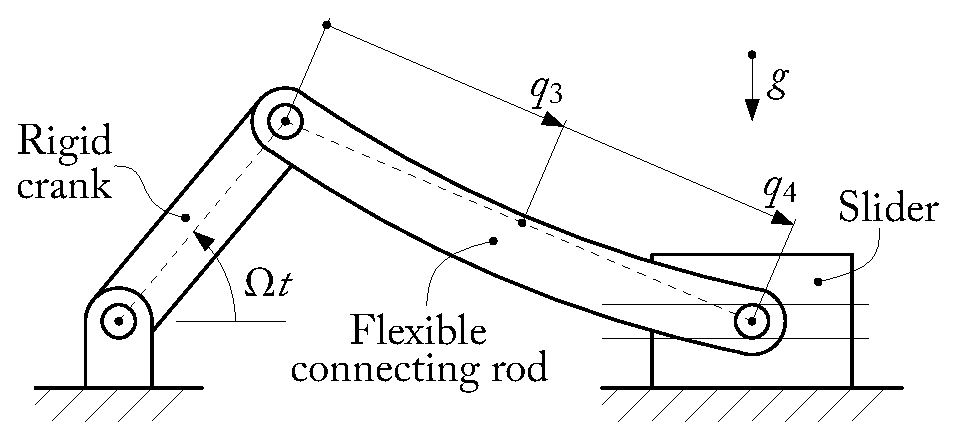
\includegraphics[width=0.475\linewidth]{flexible_slider_crank}
  \caption{Representation of the flexible slider-crank mechanism~\cite{lioen1998test, mazzia2008test}.}
  \label{chap5:fig:flexible_slider_crank}
\end{figure}

\begin{table}
  \caption{Expression complexity encountered throughout the index reduction of the flexible slider-crank mechanism problem~\cite{lioen1998test, mazzia2008test} \ac{DAE} system. \emph{Legend}: $\cf$ = functions, $\ca$ = additions, $\cm$ = multiplications, and $\cd$ = divisions.}
  \label{chap5:tab:flexible_slider_crank}
  \centering
  \resizebox{\textwidth}{!}{%
  {\footnotesize\begin{tabular}{cccc}
    \multicolumn{4}{c}{\textbf{Flexible Slider-Crank Mechanism~\cite{lioen1998test, mazzia2008test}}} \\
    \toprule
    \textbf{Original \acp{DAE}} & \multicolumn{3}{c}{$\mF = 281\cf + 10\cd + 607\cm + 144\ca$ \quad $\mh = 0$} \\
    \midrule
    \textbf{Reduction step} & $\mE$ & $\mg$ & $\ma$ \\
    \midrule
    Index-3 \acp{DAE} & $64\cf + 9\cd + 1158\cm + 167\ca$ & $395\cf + 15\cd + 5552\cm + 871\ca$ & $12\cf + 5\cm + 6\ca$ \\
    Index-2 \acp{DAE} & $64\cf + 9\cd + 1158\cm + 167\ca$ & $395\cf + 15\cd + 5552\cm + 871\ca$ & $22\cf + 10\cm + 8\ca$ \\
    Index-1 \acp{DAE} & $20\cf + 5\cd + 110\cm + 19\ca$ & $277\cf + 13\cd + 1907\cm + 326\ca$ & $\star (0.4\cf + 2.4\cm + 0.1\ca)\cdot10^{6} + 15\cd$ \\
    Index-0 \acp{DAE} & $\star (0.8\cf + 4.8\cm + 0.3\ca)\cdot10^{5} + 77\cd$ & $\star (5.8\cf + 35.7\cm + 2.2\ca)\cdot10^{6} + 1259\cd$ & $0$ \\
    \midrule
    \textbf{Reduced \acp{DAE}} & \multicolumn{3}{c}{$\star \mF = (5.8\cf + 36.2\cm + 2.2\ca)\cdot10^{6} + 1336\cd$ \quad $\star \mh = (0.5\cf + 2.4\cm + 0.1\ca)\cdot10^{6} + 15\cd$} \\
    \bottomrule
  \end{tabular}}
  }
\end{table}

\begin{table}
  \caption{Expression complexity encountered throughout the index reduction with the aid of hierarchical representation of the flexible slider-crank mechanism problem~\cite{lioen1998test, mazzia2008test} \ac{DAE} system. \emph{Legend}: $\cf$ = functions, $\cv$ = veiling variables, $\ca$ = additions, $\cm$ = multiplications, and $\cd$ = divisions.}
  \label{chap5:tab:flexible_slider_crank_veil}
  \centering
  \resizebox{\textwidth}{!}{%
  {\footnotesize\begin{tabular}{cccc}
    \multicolumn{4}{c}{\textbf{Flexible Slider-Crank Mechanism~\cite{lioen1998test, mazzia2008test}}} \\
    \toprule
    \textbf{Original \acp{DAE}} & \multicolumn{3}{c}{$\mF = 281\cf + 10\cd + 607\cm + 144\ca$ \quad $\mh = 0$} \\
    \midrule
    \textbf{Reduction step} & $\mE$ & $\mg$ & $\ma$ \\
    \midrule
    Index-3 \acp{DAE} & $28\cf + 1\cv + 7\cd + 160\cm + 28\ca$ & $91\cf + 2\cv + 8\cd + 291\cm + 44\ca$ & $12\cf + 5\cm + 6\ca$ \\
    Index-2 \acp{DAE} & $18\cf + 1\cv + 6\cd + 88\cm + 15\ca$ & $101\cf + 5\cv + 10\cd + 360\cm + 58\ca$ & $22\cf + 10\cm + 8\ca$ \\
    Index-1 \acp{DAE} & $10\cf + 1\cv + 4\cd + 39\cm + 6\ca$ & $93\cf + 4\cv + 9\cd + 294\cm + 48\ca$ & $10\cf + 2\cv + 9\cd + 82\cm + 14\ca$ \\
    Index-0 \acp{DAE} & $(0.2\cf  + 1.1\cm + 0.1\ca)\cdot10^{6} + 1171\cv + 1158\cd$ & $(0.7\cf + 3.6\cm + 0.4\ca)\cdot10^{5} + 137\cv + 1172\cd$ & $0$ \\
    \midrule
    \textbf{Reduced \acp{DAE}} & \multicolumn{3}{c}{$\mF = (0.3\cf + 1.5\cm + 0.1\ca)\cdot10^{6} + 1308\cv + 2330\cd$ \quad $\mh = 44\cf + 6\cv + 2\cd + 97\cm + 28\ca$} \\
    \bottomrule \\[0.5em]
  \end{tabular}
  }}
  {\footnotesize\begin{tabular}{cc}
    \multicolumn{2}{c}{Hierarchical representation details (9 veils)} \\
    \toprule
    \textbf{Original \acp{DAE}} & $\mv = 0$ \\
    \midrule
    \textbf{Reduction step} & $\mv$ \\
    \midrule
    Index-3 \acp{DAE} & $309\cf + 1\cv + 7\cd + 2946\cm + 485\ca$ \\
    Index-2 \acp{DAE} & $309\cf + 1\cv + 7\cd + 2946\cm + 485\ca$ \\
    Index-1 \acp{DAE} & $422\cf + 7\cv + 14\cd + 3249\cm + 541\ca$ \\
    Index-0 \acp{DAE} & $492919\cf + 63922\cv + 138\cd + 2441245\cm + 155539\ca$ \\
    \midrule
    \textbf{Reduced \acp{DAE}} & $\mv = 492919\cf + 63922\cv + 138\cd + 2441245\cm + 155539\ca$ \\
    \bottomrule
  \end{tabular}}
\end{table}

\begin{figure}[htb]
  \centering
  \small{\includetikz{figures/chapter_4/flexible_slider_crank.tex}}
  \caption{Longitudinal displacement endpoint of the in the flexible slider-crank problem~\cite{lioen1998test, mazzia2008test}. \emph{Color legend}: \textcolor{mycolor2}{$\blacksquare$} longitudinal displacement $q_3$ at the rod midpoint, and \textcolor{mycolor1}{$\blacksquare$} longitudinal displacement $q_4$ at the rod endpoint. \emph{Line legend}: \textbf{---} linear beam model, and \textbf{--~--} nonlinear beam model.}
  \label{chap5:fig:flexible_slider_crank}
\end{figure}

\begin{figure}[htb]
  \centering
  \small{\includetikz{figures/chapter_4/flexible_slider_crank_pivots.tex}}
  \caption{Representation of the two pivots of the flexible slider-crank mechanism~\cite{lioen1998test, mazzia2008test} having minimum values. \emph{Color legend}: \textcolor{mycolor1}{$\blacksquare$} pivot 1, and \textcolor{mycolor2}{$\blacksquare$} pivot 2. \emph{Line legend}: \textbf{---} linear beam model, and \textbf{--~--} nonlinear beam model.}
  \label{chap5:fig:flexible_slider_crank_pivots}
\end{figure}

\subsection{The Multi-Pendula System}

The multi-pendula system consists of a chain of $p$ coupled pendula. The first pendulum is a standard simple pendulum, while the remaining pendula are coupled to the previous one. Specifically, the tension in pendulum $i - 1$, which is represented by the Lagrange multiplier $\lambda_{i-1}$, has a small effect on the length of
pendulum $p$, for $i = 2, \dots, p$. The first-order equations of motion for the multi-pendula system are the following~\cite{nedialkov2008solvingIII}
%
\begin{equation}
  \begin{cases}
    u_1^{\prime} = x_1 \\
    v_1^{\prime} = y_1 \\
    x_1^{\prime} = -\lambda_1 x_1 \\
    y_1^{\prime} = -\lambda_1 y_1 - g \\
    x_1^2 + y_1^2 = \ell^2 \\
  \end{cases}
  \quad \text{and} \qquad
  \begin{cases}
    u_i^{\prime} = x_i \\
    v_i^{\prime} = y_i \\
    x_i^{\prime} = -\lambda_p x_i \\
    y_i^{\prime} = -\lambda_p y_i - g \\
    x_i^2 + y_i^2 = (\ell + c\lambda_{i-1})^2
  \end{cases}
  \quad \text{for} \quad i = 2, \dots, p \, \text{.}
  \label{chap5:eq:multi_pendula}
\end{equation}
%
where $x_i, y_i$ and $u_i, v_i$ are the generalized coordinates and velocities of $i$-th pendulum mass. The parameters of the multi-pendula system are chosen as $\ell = \SI{1}{\meter}$, $g = \SI{9.81}{\meter\per\second\squared}$, and $c = 0.1$. The system~\eqref{chap5:eq:multi_pendula} leads to a class of \acp{DAE} of arbitrary size $5p$ and index $2p+1$~\cite{nedialkov2008solvingIII}. \acp{IC} are chosen randomly, and the time interval is $t \in \RSI{0}{60}{\second}$.

Here, we consider up to $p = 4$ pendula, leading to a \ac{DAE} system of $20$ variables and index $9$. The computational complexities encountered during the index reduction process are summarized in Table~\ref{chap5:tab:pendula_2}, for the 2-pendula problem, Table~\ref{chap5:tab:pendula_3}, for the 3-pendula problem, Table~\ref{chap5:tab:pendula_4}, for the 4-pendula problem, and lastly, Table~\ref{chap5:tab:pendula_5}, for the 5-pendula problem. The multi-pendula systems with $p \leq 3$ exhibit low computational complexity growth during the index reduction process. However, for $p \geq 4$, there is a substantial expression swell, which makes the index reduction process time-consuming and computationally demanding, yet still feasible. The introduction of veiling variables is avoided on purpose to assess the impact of strong expression swelling on the stability of the numerical solution.
It is worth noting that with $p = 4$ the maximum computational complexity that \Maple{} can handle within a reasonable time is reached. For this reason, performing the last reduction steps for $p > 4$ requires a significant amount of time and computational resources. Furthermore, we believe that reducing the index of the \ac{DAE} system for $p > 5$ is not feasible within an acceptable time frame, even with the aid of hierarchical representation. The numerical integration results of the 5-pendula system are depicted in Figure~\ref{chap5:fig:npendula_length}, where the pendula lengths are illustrated in the time interval $t \in \RSI{0}{60}{\second}$. It must be pointed out that the numerical solution of the 5-pendula system is computed from its index-2 \ac{DAE} form, as its index-0 form demands a significant amount of computational resources and time to be solved.

\begin{table}
  \caption{Expression complexity encountered throughout the index reduction of the 2-pendula problem~\cite{nedialkov2008solvingIII} \ac{DAE} system. \emph{Legend}: $\cf$ = functions, $\ca$ = additions, $\cm$ = multiplications, and $\cd$ = divisions.}
  \label{chap5:tab:pendula_2}
  \centering
  {\footnotesize\begin{tabular}{cccc}
    \multicolumn{4}{c}{\textbf{2-Pendula~\cite{pryce1998solving}}} \\
    \toprule
    \textbf{Original \acp{DAE}} & \multicolumn{3}{c}{$\mF = 33\cf + 15\cm + 15\ca$ \quad $\mh = 0$} \\
    \midrule
    \textbf{Reduction step} & $\mE$ & $\mg$ & $\ma$ \\
    \midrule
    Index-5 \acp{DAE} & $0$                  & $12\cf + 8\cm + 2\ca$ & $6\cf + 12\cm + 6\ca$ \\
    Index-4 \acp{DAE} & $1\cf + 5\cm + 1\ca$ & $16\cf + 12\cm + 3\ca$ & $4\cf + 4\cm + 1\ca$ \\
    Index-3 \acp{DAE} & $1\cf + 5\cm + 1\ca$ & $16\cf + 12\cm + 3\ca$ & $7\cf + 12\cm + 4\ca$ \\
    Index-2 \acp{DAE} & $1\cf + 5\cm + 1\ca$ & $16\cf + 12\cm + 3\ca$ & $18\cf + 2\cd + 30\cm + 9\ca$ \\
    Index-1 \acp{DAE} & $1\cf + 5\cm + 1\ca$ & $16\cf + 12\cm + 3\ca$ & $118\cf + 2\cd + 283\cm + 72\ca$ \\
    Index-0 \acp{DAE} & $555\cf + 21\cd + 1213\cm + 287\ca$ & $16\cf + 12\cm + 3\ca$ & $0$ \\
    \midrule
    \textbf{Reduced \acp{DAE}} & \multicolumn{3}{c}{
    $\mF = 482\cf + 2\cd + 807\cm + 229\ca$ \quad $\mh = 153\cf + 4\cd + 341\cm + 92\ca$} \\
    \bottomrule
  \end{tabular}}
\end{table}

\begin{table}
  \caption{Expression complexity encountered throughout the index reduction of the 3-pendula problem~\cite{nedialkov2008solvingIII} \ac{DAE} system. \emph{Legend}: $\cf$ = functions, $\ca$ = additions, $\cm$ = multiplications, and $\cd$ = divisions.}
  \label{chap5:tab:pendula_3}
  \centering
  {\footnotesize\begin{tabular}{cccc}
    \multicolumn{4}{c}{\textbf{3-Pendula~\cite{nedialkov2008solvingIII}}} \\
    \toprule
    \textbf{Original \acp{DAE}} & \multicolumn{3}{c}{$\mF = 50\cf + 23\cm + 23\ca$ \quad $\mh = 0$} \\
    \midrule
    \textbf{Reduction step} & $\mE$ & $\mg$ & $\ma$ \\
    \midrule
    Index-7 \acp{DAE} & $0$                   & $18\cf + 12\cm + 3\ca$ & $10\cf + 21\cm + 10\ca$ \\
    Index-6 \acp{DAE} & $2\cf + 10\cm + 2\ca$ & $26\cf + 20\cm + 5\ca$ & $4\cf + 4\cm + 1\ca$ \\
    Index-5 \acp{DAE} & $2\cf + 10\cm + 2\ca$ & $26\cf + 20\cm + 5\ca$ & $7\cf + 12\cm + 4\ca$ \\
    Index-4 \acp{DAE} & $2\cf + 10\cm + 2\ca$ & $26\cf + 20\cm + 5\ca$ & $18\cf + 2\cd + 30\cm + 9\ca$ \\
    Index-3 \acp{DAE} & $2\cf + 10\cm + 2\ca$ & $26\cf + 20\cm + 5\ca$ & $118\cf + 2\cd + 283\cm + 72\ca$ \\
    Index-2 \acp{DAE} & $2\cf + 10\cm + 2\ca$ & $26\cf + 20\cm + 5\ca$ & $992\cf + 3\cd + 2077\cm + 479\ca$ \\
    Index-1 \acp{DAE} & $2\cf + 10\cm + 2\ca$ & $26\cf + 20\cm + 5\ca$ & $6824\cf + 3\cd + 17665\cm + 4030\ca$ \\
    Index-0 \acp{DAE} & $54152\cf + 51\cd + 136388\cm + 28945\ca$ & $26\cf + 20\cm + 5\ca$ & $0$ \\
    \midrule
    \textbf{Reduced \acp{DAE}} & \multicolumn{3}{c}{
    $\mF = 28319\cf + 3\cd + 64295\cm + 15806\ca$ \quad $\mh = 7973\cf + 10\cd + 20092\cm + 4605\ca$} \\
    \bottomrule
  \end{tabular}}
\end{table}

\begin{table}
  \caption{Expression complexity encountered throughout the index reduction of the 4-pendula problem~\cite{nedialkov2008solvingIII} \ac{DAE} system. \emph{Legend}: $\cf$ = functions, $\ca$ = additions, $\cm$ = multiplications, and $\cd$ = divisions.}
  \label{chap5:tab:pendula_4}
  \centering
  {\footnotesize\begin{tabular}{cccc}
    \multicolumn{4}{c}{\textbf{4-Pendula~\cite{nedialkov2008solvingIII}}} \\
    \toprule
    \textbf{Original \acp{DAE}} & \multicolumn{3}{c}{$\mF = 67\cf + 31\cm + 31\ca$ \quad $\mh = 0$} \\
    \midrule
    \textbf{Reduction step} & $\mE$ & $\mg$ & $\ma$ \\
    \midrule
    Index-9 \acp{DAE} & $0$                   & $24\cf + 16\cm + 4\ca$ & $14\cf + 30\cm + 14\ca$ \\
    Index-8 \acp{DAE} & $3\cf + 15\cm + 3\ca$ & $36\cf + 28\cm + 7\ca$ & $4\cf + 4\cm + 1\ca$ \\
    Index-7 \acp{DAE} & $3\cf + 15\cm + 3\ca$ & $36\cf + 28\cm + 7\ca$ & $7\cf + 12\cm + 4\ca$ \\
    Index-6 \acp{DAE} & $3\cf + 15\cm + 3\ca$ & $36\cf + 28\cm + 7\ca$ & $18\cf + 2\cd + 30\cm + 9\ca$ \\
    Index-5 \acp{DAE} & $3\cf + 15\cm + 3\ca$ & $36\cf + 28\cm + 7\ca$ & $118\cf + 2\cd + 283\cm + 72\ca$ \\
    Index-4 \acp{DAE} & $3\cf + 15\cm + 3\ca$ & $36\cf + 28\cm + 7\ca$ & $992\cf + 3\cd + 2077\cm + 479\ca$ \\
    Index-3 \acp{DAE} & $3\cf + 15\cm + 3\ca$ & $36\cf + 28\cm + 7\ca$ & $6824\cf + 3\cd + 17665\cm + 4030\ca$ \\
    Index-2 \acp{DAE} & $3\cf + 15\cm + 3\ca$ & $36\cf + 28\cm + 7\ca$ & $(4.8\cf + 4\cd + 11.9\cm + 2.7\ca)\cdot10^{5}$ \\
    Index-1 \acp{DAE} & $3\cf + 15\cm + 3\ca$ & $36\cf + 28\cm + 7\ca$ & $\star (3.0\cf + 14.9\cm + 0.4\ca)\cdot10^{6} + 4\cd$ \\
    Index-0 \acp{DAE} & $\star (3.0\cf + 14.7\cm + 0.4\ca)\cdot10^{7} + 92\cd$ & $30\cf + 28\cm + 7\ca$ & $0$ \\
    \midrule
    \textbf{Reduced \acp{DAE}} & \multicolumn{3}{c}{
    $\star \mF = (3.0\cf + 14.7\cm + 0.4\ca)\cdot10^{7} + 92\cd$ \quad $\star \mh = (3.1\cf + 15.1\cm + 0.5\ca)\cdot10^{6} + 18\cd$} \\
    \bottomrule
  \end{tabular}}
\end{table}

\begin{table}
  \caption{Expression complexity encountered throughout the index reduction of the 5-pendula problem~\cite{nedialkov2008solvingIII} \ac{DAE} system. \emph{Legend}: $\cf$ = functions, $\ca$ = additions, $\cm$ = multiplications, and $\cd$ = divisions.}
  \label{chap5:tab:pendula_5}
  \centering
  {\footnotesize\begin{tabular}{cccc}
    \multicolumn{4}{c}{\textbf{5-Pendula~\cite{nedialkov2008solvingIII}}} \\
    \toprule
    \textbf{Original \acp{DAE}} & \multicolumn{3}{c}{$\mF = 84\cf + 39\cm + 39\ca$ \quad $\mh = 0$} \\
    \midrule
    \textbf{Reduction step} & $\mE$ & $\mg$ & $\ma$ \\
    \midrule
    Index-11 \acp{DAE} & $0$                   & $30\cf + 20\cm + 5\ca$ & $18\cf + 39\cm + 18\ca$ \\
    Index-10 \acp{DAE} & $4\cf + 20\cm + 4\ca$ & $46\cf + 36\cm + 9\ca$ & $4\cf + 4\cm + 1\ca$ \\
    Index-9 \acp{DAE}  & $4\cf + 20\cm + 4\ca$ & $46\cf + 36\cm + 9\ca$ & $7\cf + 12\cm + 4\ca$ \\
    Index-8 \acp{DAE}  & $4\cf + 20\cm + 4\ca$ & $46\cf + 36\cm + 9\ca$ & $18\cf + 2\cd + 30\cm + 9\ca$ \\
    Index-7 \acp{DAE}  & $4\cf + 20\cm + 4\ca$ & $46\cf + 36\cm + 9\ca$ & $118\cf + 2\cd + 283\cm + 72\ca$ \\
    Index-6 \acp{DAE}  & $4\cf + 20\cm + 4\ca$ & $46\cf + 36\cm + 9\ca$ & $992\cf + 3\cd + 2077\cm + 479\ca$ \\
    Index-5 \acp{DAE}  & $4\cf + 20\cm + 4\ca$ & $46\cf + 36\cm + 9\ca$ & $6824\cf + 3\cd + 17665\cm + 4030\ca$ \\
    Index-4 \acp{DAE}  & $4\cf + 20\cm + 4\ca$ & $46\cf + 36\cm + 9\ca$ & $(4.8\cf + 4\cd + 11.9\cm + 2.7\ca)\cdot10^{5}$ \\
    Index-3 \acp{DAE}  & $4\cf + 20\cm + 4\ca$ & $46\cf + 36\cm + 9\ca$ & $\star (3.0\cf + 14.9\cm + 0.4\ca)\cdot10^{6} + 4\cd$ \\
    Index-2 \acp{DAE}  & $4\cf + 20\cm + 4\ca$ & $46\cf + 36\cm + 9\ca$ & $\star (5.1\cf + 4.0\cm + 1.3\ca)\cdot10^{7} + 5\cd$ \\
    Index-1 \acp{DAE}  & $4\cf + 20\cm + 4\ca$ & $46\cf + 36\cm + 9\ca$ & $\star (9.1\cf + 11.3\cm + 5.9\ca)\cdot10^{7} + 5\cd$ \\
    Index-0 \acp{DAE}  & $\star (8.8\cf + 7.2\cm + 1.0\ca)\cdot10^{8} + 5\cd$ & $46\cf + 36\cm + 9\ca$ & $0$ \\
    \midrule
    \textbf{Reduced \acp{DAE}} & \multicolumn{3}{c}{
    $\star \mF = \star (8.8\cf + 7.2\cm + 1.0\ca)\cdot10^{8} + 5\cd$ \quad $\star \mh = (9.2\cf + 6.5\cm + 1.0\ca)\cdot10^{7} + 18\cd$} \\
    \bottomrule
  \end{tabular}}
\end{table}

\begin{figure}[htb]
  \centering
  \small{\includetikz{figures/chapter_4/npendula_length.tex}}
  \caption{Pendula lengths of the multi-pendula problem~\cite{nedialkov2008solvingIII} (up to 5 pendula). \emph{Legend}: \textcolor{mycolor1}{$\blacksquare$} 1\textsuperscript{st} pendulum length $\ell_1 = \ell$, \textcolor{mycolor2}{$\blacksquare$} 2\textsuperscript{nd} pendulum length $\ell_2 = \ell + c\lambda_1$, \textcolor{mycolor3}{$\blacksquare$} 3\textsuperscript{rd} pendulum length $\ell_3 = \ell + c\lambda_2$, \textcolor{mycolor4}{$\blacksquare$} 4\textsuperscript{th} pendulum length $\ell_4 = \ell + c\lambda_3$, and \textcolor{mycolor5}{$\blacksquare$} 5\textsuperscript{th} pendulum length $\ell_5 = \ell + c\lambda_4$.}
  \label{chap5:fig:npendula_length}
\end{figure}

\subsection{Double-Wishbone Suspension System}

As a final example for this application field, we consider a double-wishbone suspension system.

\subsubsection{Suspension System Modeling}

Double A-arm or double wishbone suspensions are independent suspension systems widely used in the automotive industry, especially in high-performance vehicles, due to their superior handling characteristics. The studied double A-arm suspension system, shown in Figure~\ref{chap5:fig:suspension_render} is characterized by two A-shaped arms, one upper and one lower, connected to the chassis at one end and to the wheel carrier at the other end forming, together with the tie rod, the principal kinematic chain of the suspension system. A second kinematic chain is formed by the push rod and the rocker, which transfer the vertical load from the wheel carrier to the shock absorber.

\begin{figure}[htb]
  \begin{minipage}[c]{0.485\linewidth}
    \centering
    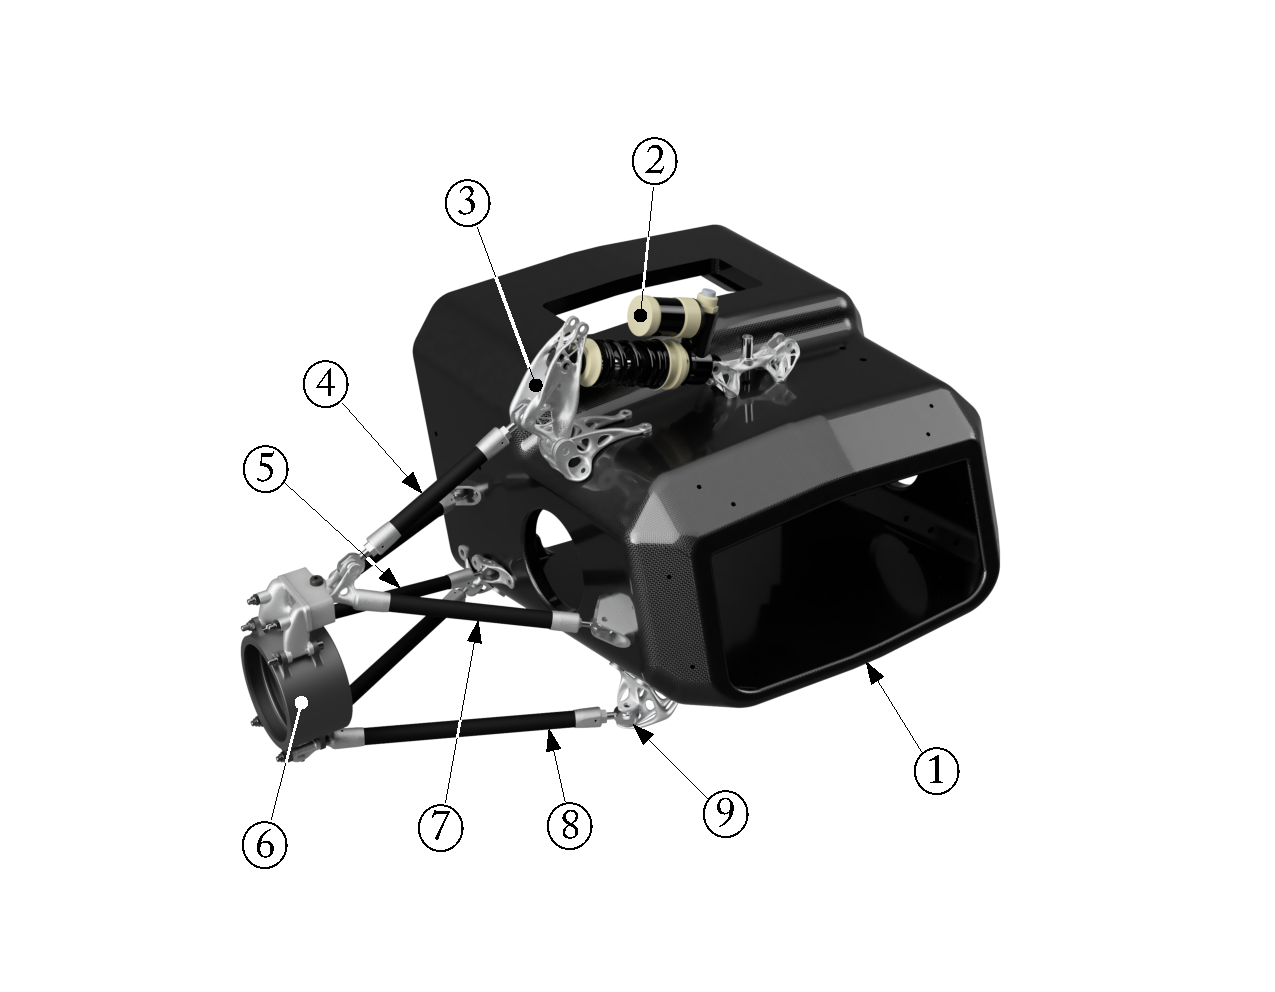
\includegraphics[width=1.0\textwidth, trim={3.0cm 1.5cm 4.0cm 1.7cm}, clip]{figures/chapter_4/suspension_render.eps}
  \end{minipage}
  %\hfill
  \begin{minipage}[c]{0.45\linewidth}
    \centering
    \small{\begin{tabular}{ccc}
      \toprule
      \multirow{2}{*}{\textbf{\#}} & \multirow{2}{*}{\textbf{Component}} & \textbf{\TrussMe{}} \\
      & & \textbf{type} \\
      \midrule
      \circled{\small{1}} & Carbon fiber cell & Rigid support    \\[1.25mm]
      \circled{\small{2}} & Shock absorber    & Constrained node \\[1.25mm]
      \circled{\small{3}} & Rocker            & Generic element  \\[1.25mm]
      \circled{\small{4}} & Push rod          & Rod element      \\[1.25mm]
      \circled{\small{5}} & Tie rod           & Rod element      \\[1.25mm]
      \circled{\small{6}} & Wheel carrier     & Generic element  \\[1.25mm]
      \circled{\small{7}} & Upper wishbone    & Beam elements    \\[1.25mm]
      \circled{\small{8}} & Lower wishbone    & Beam elements    \\[1.25mm]
      \circled{\small{9}} & Rod end           & Compliant node    \\
      \bottomrule
    \end{tabular}}
  \end{minipage}
  \caption{Rendering and description of the \TrussMe{} elements \citep{trussme} used to model the rear left double wishbone suspension of the Formula SAE \textit{E-Agle Trento Racing Team} vehicle~\citep{eagle}.}
  \label{chap5:fig:suspension_render}
\end{figure}

In this example, the double A-arm suspension compliance is modeled using macro elements, which are modeled through the \TrussMe{} package~\cite{trussme}, which is a \Maple{} package for the symbolic modeling of compliant structures. Details on the modeling of the compliant elements are reported in Appendix~\ref{app4:trussme}. With the approach there presented, two suspension compliance models are generated one does not include the bushings compliance, while the other does. The linear systems have different sizes depending on the number of \acp{DOF} considered. In the case of the suspension without bushings, the system is composed of 78 \acp{DOF}, and has the following form
%
\begin{equation}
  \begin{bmatrix}
    \m{K}_{ff ,\, 42 \times 42}(\mathbb{R}) & \m{K}_{fs ,\, 42 \times 36}(\mathbb{R}) \\
    \m{K}_{sf ,\, 36 \times 42}(\mathbb{R}) & \m{K}_{ss ,\, 36 \times 36}(\mathbb{R})
  \end{bmatrix} \begin{bmatrix}
    \m{d}_{f ,\, 42 \times 1}(\mathbb{R}) \\ \m{d}_{s ,\, 36 \times 1}(\mathbb{R})
  \end{bmatrix} = \begin{bmatrix}
    \m{f}_{f ,\, 42 \times 1}(\mathbb{R}) \\ \m{f}_{s ,\, 36 \times 1}(\mathbb{R})
  \end{bmatrix}
  \, \text{.}
\end{equation}
%
On the other hand, the suspension model with the bushings influence is composed of 138 \acp{DOF}
%
\begin{equation}
  \begin{bmatrix}
    \m{K}_{ff ,\, 72 \times 72}(\mathbb{R}) & \m{K}_{fs ,\, 72 \times 66}(\mathbb{R}) \\
    \m{K}_{sf ,\, 66 \times 72}(\mathbb{R}) & \m{K}_{ss ,\, 66 \times 66}(\mathbb{R})
  \end{bmatrix} \begin{bmatrix}
    \m{d}_{f ,\, 72 \times 1}(\mathbb{R}) \\ \m{d}_{s ,\, 66 \times 1}(\mathbb{R})
  \end{bmatrix} = \begin{bmatrix}
    \m{f}_{f ,\, 72 \times 1}(\mathbb{R}) \\ \m{f}_{s ,\, 66 \times 1}(\mathbb{R})
  \end{bmatrix}
  \, \text{,}
\end{equation}
%
where the additional 60 \acp{DOF} are related to the compliance of the bushings. Both systems are solved using the technique presented in Appendix~\ref{app4:trussme}, which given the generic compliant mechanism described by the linear system of equations
%
\begin{equation}
  \label{chap5:eq:macrofe}
  \underbrace{\begin{bmatrix}
    \m{K}_{ff} & \m{K}_{fs} \\
    \m{K}_{sf} & \m{K}_{ss}
  \end{bmatrix}}_{\textstyle\m{K}} \underbrace{\begin{bmatrix}
    \m{d}_{f} \\ \m{d}_{s}
  \end{bmatrix}}_{\textstyle\m{d}} = \underbrace{\begin{bmatrix}
    \m{f}_{f} \\ \m{f}_{s}
  \end{bmatrix}}_{\textstyle\m{f}} \, \text{,}
  %
  \qquad \text{is sequentially solved as} \qquad
  %
  \begin{aligned}
    \m{d}_{f} &= \m{K}_{ff}^{-1}\left(\m{f}_{f} - \m{K}_{fs}\m{d}_{s}\right) \, \text{,} \\
    \m{f}_{s} &= \m{K}_{sf}\m{d}_{f} + \m{K}_{ss}\m{d}_{s} \, \text{,}
  \end{aligned}
\end{equation}
%
where subscripts $s$ and $f$ indicate respectively the specified and the free \acp{DOF}. Notice that the free and the specified \acp{DOF} are those that are and are not constrained by the \acp{BC}, respectively.

The dynamic characteristic of the system is modeled through a \ac{DAE} system of the following type:
%
\begin{subequations}
  \label{chap5:eq:daes}
  \begin{empheq}[left = {\empheqlbrace}, right = {\, \text{,}}]{align}
    & \m{y} = \m{q} + \m{d} \label{chap5:eq:sy} \\
    & \m{M}(\m{y}) \m{y}^{\prime\prime} + \m{r}(\m{q}, \m{q}^\prime, \m{d}, \m{d}^\prime) = \m{f}(t) \label{chap5:eq:cr} \\
    & \boldsymbol{\Phi}_{\m{q}}(\m{q})^\top \boldsymbol{\lambda} = \m{r}(\m{q}, \m{q}^\prime, \m{d}, \m{d}^\prime) + \m{b}(\m{q}, \m{q}^\prime, t) \label{chap5:eq:em} \\
    & \boldsymbol{\Phi}(\m{q}) = \m{0} \label{chap5:eq:bc}
  \end{empheq} \\[-2.5em]
  \begin{equation}
    \label{chap5:eq:emf}
    \text{with} \quad \m{r}(\m{q}, \m{q}^\prime, \m{d}, \m{d}^\prime) = \m{K}_c(\m{q}) \m{d} + \m{C}_c(\m{q}) \m{d}^\prime \text{,}
  \end{equation}
\end{subequations}
%
where $\m{q}$ is the state vector, and $t$ is the time. The quantity $\m{d}$ represents the compliance contribution of the mechanism members' deformation. States and deformations are conveniently condensed in a single variable $\m{y}$ as in~\eqref{chap5:eq:sy}. Equation~\eqref{chap5:eq:cr} represents the compliance contribution to the dynamics of the system, where $\m{K}_c$, and $\m{C}_c$ are the stiffness and damping matrices of the compliant bodies, respectively. The matrix $\m{M}$ represents the mass of the mechanism, while $\m{f}$ is the vector of external forces. For convenience, we collect $\m{r}$ in Equation~\eqref{chap5:eq:emf} as the vector of internal forces at the compliant joint. Notice that the product $\m{K}_c(\m{q}) \m{d}$ can be computed through the symbolic solution of the linear systems~\eqref{chap5:eq:macrofe}. Equation~\eqref{chap5:eq:em} represents the equilibrium equations between the rigid and compliant parts of the suspension. Specifically, $\boldsymbol{\Phi}_{\m{q}}$ is the Jacobian matrix of the constraint vector $\boldsymbol{\Phi}$ with respect to the coordinates $\m{q}$, while $\m{b}$ is the vector of external forces applied to the rigid part of the suspension. Lastly, Equation~\eqref{chap5:eq:bc} represents the kinematic constraints of the system. The pick-up points of the modeled suspension are reported in Table~\ref{chap5:tab:positions}. It is possible to derive the lengths of the various elements from these coordinates and to impose constraints to ensure a proper assembling of the mechanism. Components and materials specifications are reported in Tables~\ref{chap5:tab:components} and~\ref{chap5:tab:materials}, respectively.

It is important to note that one may consider the compliance contribution as a superposed effect. To this end, we first assume that the influence of the members' deformation $\m{d}$ is small with respect to the dimensions of the mechanism itself, and thus to the state vector $\m{q}$, \ie{}, $\m{d} \ll \m{q}$. From~\eqref{chap5:eq:sy} it follows that $\m{M}(\m{y}) \approx \m{M}(\m{q})$. It is then possible to split the resolution of the \acp{DAE}~\eqref{chap5:eq:daes} into two stages. Firstly, the implicit differential equation~\eqref{chap5:eq:em} and the manifold~\eqref{chap5:eq:bc} are integrated. Nonetheless, these equations are of an index-3 \ac{MB} \acp{DAE} system of the type~\eqref{chap5:eq:mbd_fo}, which can be reduced to an index-0 or index-1 \acp{DAE} system and solved as above explained. Then, the second stage consists of adding the stationary contribution of the members' deformation $\m{d}$ to the state vector $\m{q}$, that is $\m{y} = \m{q} + \m{d} = \m{q} + \m{K}_c(\m{q})^{-1} (\m{f}(t) - \m{M}(\m{q})\m{q}^{\prime\prime})$.

\begin{table}[htb]
  \caption[Table]{Suspension pick-up points' coordinates in the nominal position.}
  \label{chap5:tab:positions}
  \centering
  \small{\begin{tabular}{cccccc}
    \toprule
    \multirow{2.5}{*}{\shortstack{\textbf{Pick-up} \\ \textbf{point name}}} &
    \multicolumn{2}{c}{\multirow{2.5}{*}{\textbf{Constrained elements}}} &
    \multicolumn{3}{c}{\textbf{Coordinates}} \\ \cmidrule(r{4pt}l{4pt}){4-6}
    & & & $x$~(\USI{\milli\meter}) & $y$~(\USI{\milli\meter}) & $z$~(\USI{\milli\meter}) \\
    \midrule
    $P_{1}$  & Chassis       & Upper-front rod & $-719$  & $270$ & $240$ \\ %(3)
    $P_{2}$  & Chassis       & Upper-rear rod  & $-1010$ & $265$ & $225$ \\ %(4)
    $P_{3}$  & Chassis       & Lower-front rod & $-730$  & $265$ & $120$ \\ %(1)
    $P_{4}$  & Chassis       & Lower-rear rod  & $-1010$ & $235$ &  $98$ \\ %(2)
    $P_{5}$  & Chassis       & Tie rod         & $-775$  & $265$ & $163$ \\ %(5)
    $P_{6}$  & Chassis       & Rocker          & $-895$  & $243$ & $375$ \\ %(13)
    $P_{7}$  & Chassis       & Shock absorber  & $-895$  &  $50$ & $412$ \\ %(15)
    $P_{8}$  & Wheel carrier & Upper-front rod & $-895$  & $517$ & $293$ \\ %(6)
    $P_{9}$  & Wheel carrier & Upper-rear rod  & $-895$  & $517$ & $293$ \\ %(6)
    $P_{10}$ & Wheel carrier & Lower-front rod & $-885$  & $550$ & $120$ \\ %(7)
    $P_{11}$ & Wheel carrier & Lower-rear rod  & $-885$  & $550$ & $120$ \\ %(7)
    $P_{12}$ & Wheel carrier & Tie rod         & $-790$  & $532$ & $198$ \\ %(8)
    $P_{13}$ & Rocker        & Shock absorber  & $-895$  & $236$ & $466$ \\ %(14)
    $P_{14}$ & Rocker        & Push rod        & $-895$  & $280$ & $418$ \\ %(12)
    $P_{15}$ & Push rod      & Wheel carrier   & $-895$  & $479$ & $312$ \\ %(11)
    \bottomrule
  \end{tabular}}
\end{table}

\noindent
\begin{minipage}[c]{0.485\linewidth}
  \centering
  \captionof{table}{Suspension shock absorber and wheel specifications used in \Ansys{} and \TrussMe{} simulations.}
  \label{chap5:tab:components}
  \centering
  \small{\begin{tabular}{ccc}
    \toprule
    \textbf{Component} & \textbf{Property} & \textbf{Quantity} \\
    \midrule
    \multirow{4}{*}{\shortstack{Shock \\ absorber}}
    & Stiffness   & \SSI{255}{\kilo\newton\per\meter} \\
    & Damping     & \SSI{500}{\newton\second\per\meter} \\
    & Travel      & \SSI{0.06}{\meter} \\
    \midrule
    \multirow{3}{*}{\shortstack{Wheel \\ body}}
    & Mass          & \SSI{12.5}{\kilo\gram} \\
    & Inertia diam. & \SSI{0.21}{\kilo\gram\meter}\textsuperscript{2} \\
    & Inertia axial & \SSI{0.42}{\kilo\gram\meter}\textsuperscript{2} \\
    \bottomrule
  \end{tabular}}
\end{minipage}
\hfill
\begin{minipage}[c]{0.485\linewidth}
  \centering
  \captionof{table}{Properties of suspension materials used in \Ansys{} and \TrussMe{} simulations, where $E$ is the Young modulus, $\nu$ is the Poisson ratio, and $\rho$ is the density.}
  \label{chap5:tab:materials}
  \centering
  \small{\begin{tabular}{cccc}
    \toprule
    \multirow{2.5}{*}{\textbf{Material}} & \multicolumn{3}{c}{\textbf{Properties}} \\ \cmidrule(r{4pt}l{4pt}){2-4}
    & $E$~(\USI{\giga\pascal}) & $\nu$\,(--) & $\rho$~(\USI{\kilo\gram\meter}\textsuperscript{3}) \\
    \midrule
    AISI 1045     & $210.0$ & $0.30$ & $7800$ \\
    AISI 316L     & $196.0$ & $0.25$ & $7990$ \\
    Ergal 7075-T6 & $\phantom{1}71.7$ & $0.33$ & $2810$ \\
    Carbon fiber  & $150.0$ & $0.34$ & $1500$ \\
    Epoxy glue    & $1.718$ & $0.33$ & $1440$ \\
    \bottomrule
  \end{tabular}}
\end{minipage}

\subsubsection{System Solution}

Prior to any analyses, the \ac{DAE} system is handled to \Indigo{} for index reduction. For this purpose, the system is reduced to a system of \acp{ODE} and the computational complexities encountered during the reduction process are reported in Table~\ref{chap5:tab:suspension}. Notice the substantial increase in the expression complexity of the reduced system in the last two reduction steps despite the simplification capabilities of \Maple{}, which indicates a high level of inherent expression swell.

\begin{table}
  \caption{Expression complexity encountered throughout the index reduction with the aid of hierarchical representation of the double-wishbone suspension system \ac{DAE} system. \emph{Legend}: $\cf$ = functions, $\cv$ = veiling variables, $\ca$ = additions, $\cm$ = multiplications, and $\cd$ = divisions.}
  \label{chap5:tab:suspension}
  \centering
  {\footnotesize\begin{tabular}{cccc}
    \multicolumn{4}{c}{\textbf{Double-Wishbone Suspension}} \\
    \toprule
    \textbf{Original \acp{DAE}} & \multicolumn{3}{c}{$\mF = 845\cf + 610\cm + 465\ca$ \quad $\mh = 0$} \\
    \midrule
    \textbf{Reduction step} & $\mE$ & $\mg$ & $\ma$ \\
    \midrule
    Index-3 \acp{DAE} & $16\cf + 15\cm + 4\ca$ & $217\cf + 3\cv + 165\cm + 104\ca$ & $252\cf + 154\cm + 128\ca$ \\
    Index-2 \acp{DAE} & $16\cf + 15\cm + 4\ca$ & $217\cf + 3\cv + 165\cm + 104\ca$ & $161\cf + 3\cv + 105\cm + 49\ca$ \\
    Index-1 \acp{DAE} & $14\cf + 14\cm + 4\ca$ & $223\cf + 4\cv + 1\cd + 170\cm + 104\ca$ & $7\cv + 6\ca$ \\
    Index-0 \acp{DAE} & $104\cf + 155\cv + 15\cd + 160\cm + 81\ca$ & $223\cf + 11\cv + 1\cd + 170\cm + 105\ca$ & $0$ \\
    \midrule
    \textbf{Reduced \acp{DAE}} & \multicolumn{3}{c}{$\mF = 551\cf + 144\cv + 7\cd + 542\cm + 269\ca$ \quad $\mh = 413\cf + 10\cv + 259\cm + 183\ca$} \\
    \bottomrule \\[0.5em]
  \end{tabular}
  \begin{tabular}{cc}
    \multicolumn{2}{c}{Hierarchical representation details (151 veils)} \\
    \toprule
    \textbf{Original \acp{DAE}} & $\mv = 0$ \\
    \midrule
    \textbf{Reduction step} & $\mv$ \\
    \midrule
    Index-3 \acp{DAE} & $320\cf + 1\cv + 264\cm + 212\ca$ \\
    Index-2 \acp{DAE} & $716\cf + 1\cv + 582\cm + 440\ca$ \\
    Index-1 \acp{DAE} & $6391\cf + 28\cv + 10\cd + 5385\cm + 3301\ca$ \\
    Index-0 \acp{DAE} & $119901\cf + 3765\cv + 192\cd + 108637\cm + 64865\ca$ \\
    \midrule
    \textbf{Reduced \acp{DAE}} & $\mv = 119901\cf + 3765\cv + 192\cd + 108637\cm + 64865\ca$ \\
    \bottomrule
  \end{tabular}}
\end{table}

After the reduction process, the reduced system is numerically solved generating appropriate code for the \Simulink{} environment. The system is also reproduced in \Ansys{} for comparison and validation. The first test that is carried out aims to verify the accuracy of the reduced system and to predict the impact of compliance on the system dynamics. The results of the frequency response analysis are shown in Figure~\ref{chap5:fig:suspension_dynamic_results}. The results show that the \Simulink{} multi-body simulation with full compliance dynamics contribution and the \Ansys{} \ac{FE} modal analysis are in good agreement and the first three modal shapes, which are shown in Figure~\ref{chap5:fig:suspension_modes}, are well captured by the reduced system with full compliance dynamics contribution. Conversely, the reduced system with steady-state compliance dynamics contribution is not able to capture the first three modal shapes of the suspension. This result, despite expected, also introduces a zero along the suspension moving direction in the frequency response of the system, which is not present in the full compliance dynamics contribution. The following considerations can be made from these results: the compliance of the suspension system has a significant impact on the system dynamics for high-frequency analyses, and the reduced system with full compliance dynamics contribution can capture the system dynamics accurately. For computationally efficient simulations, the reduced system with steady-state compliance dynamics contribution can be used to capture the system dynamics accurately under the assumption that the suspension system is forced by low-frequency inputs.

\begin{figure}[htb]
  \centering
  \begin{subfigure}[c]{0.225\textwidth}
    \centering
    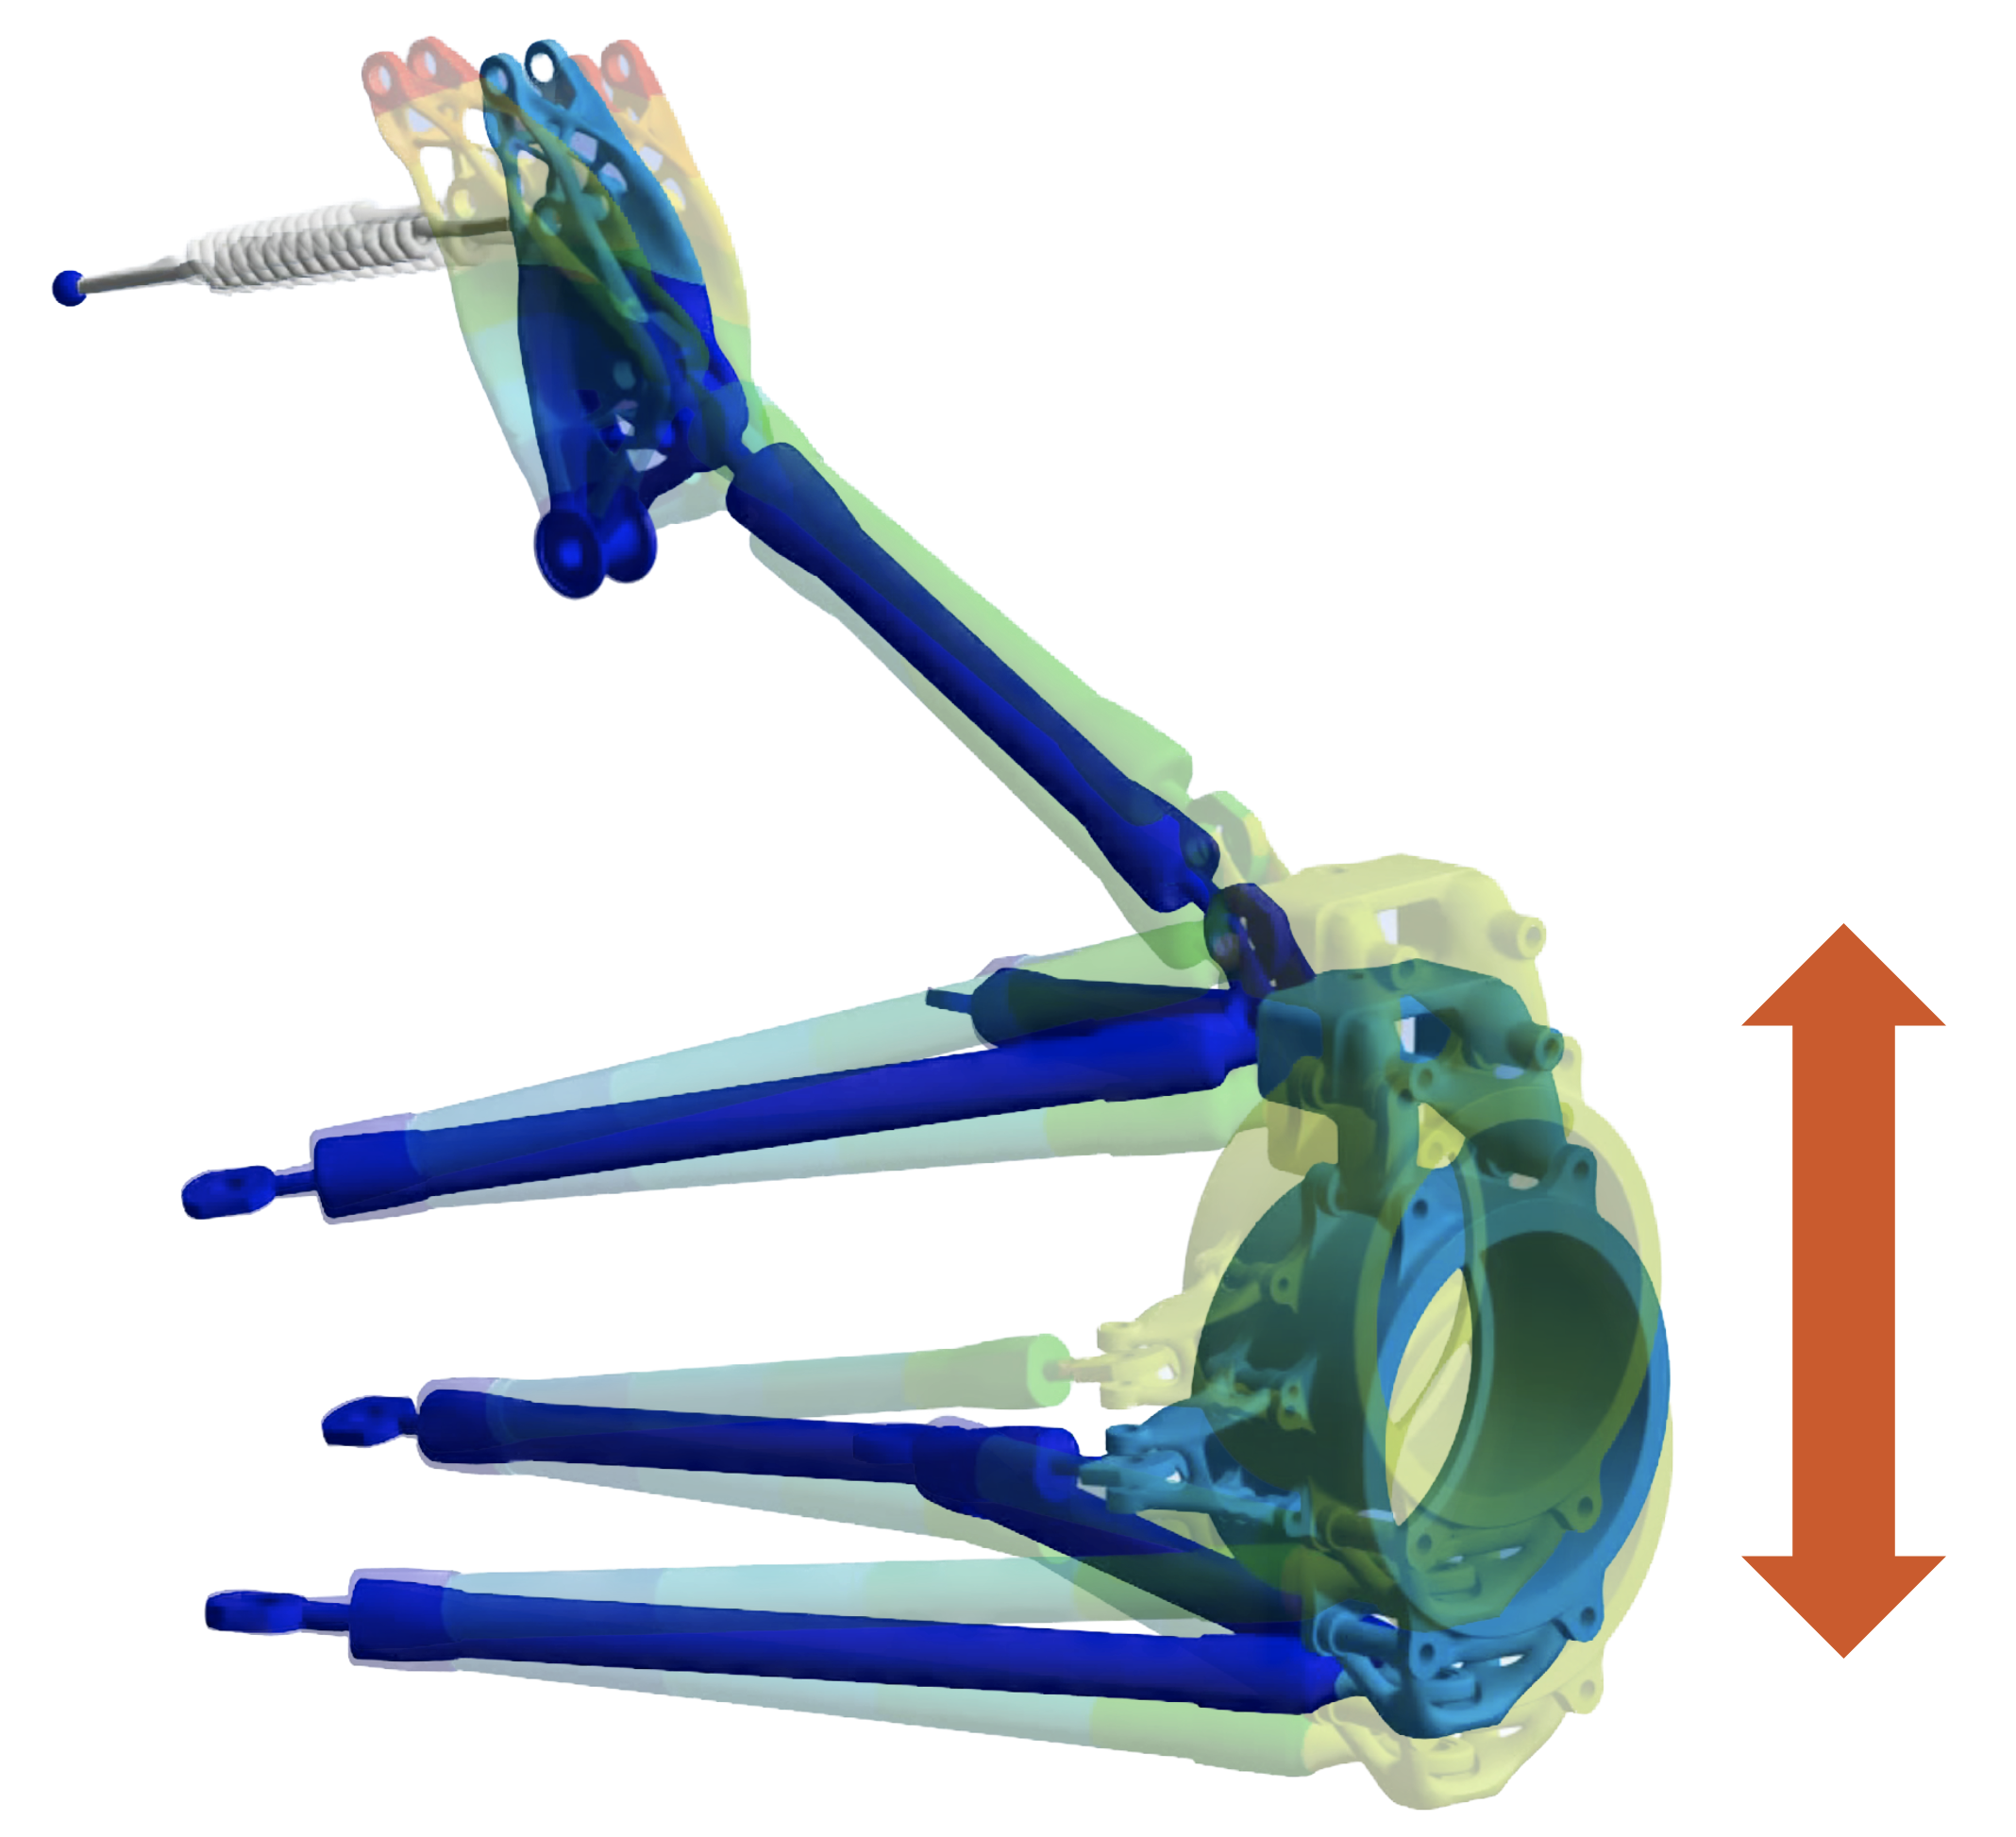
\includegraphics[width=1.0\linewidth]{figures/chapter_4/suspension_mode_1}
    \caption{$f_1 = \SSI{7.6}{\hertz}$}
  \end{subfigure}
  \begin{subfigure}[c]{0.225\textwidth}
    \centering
    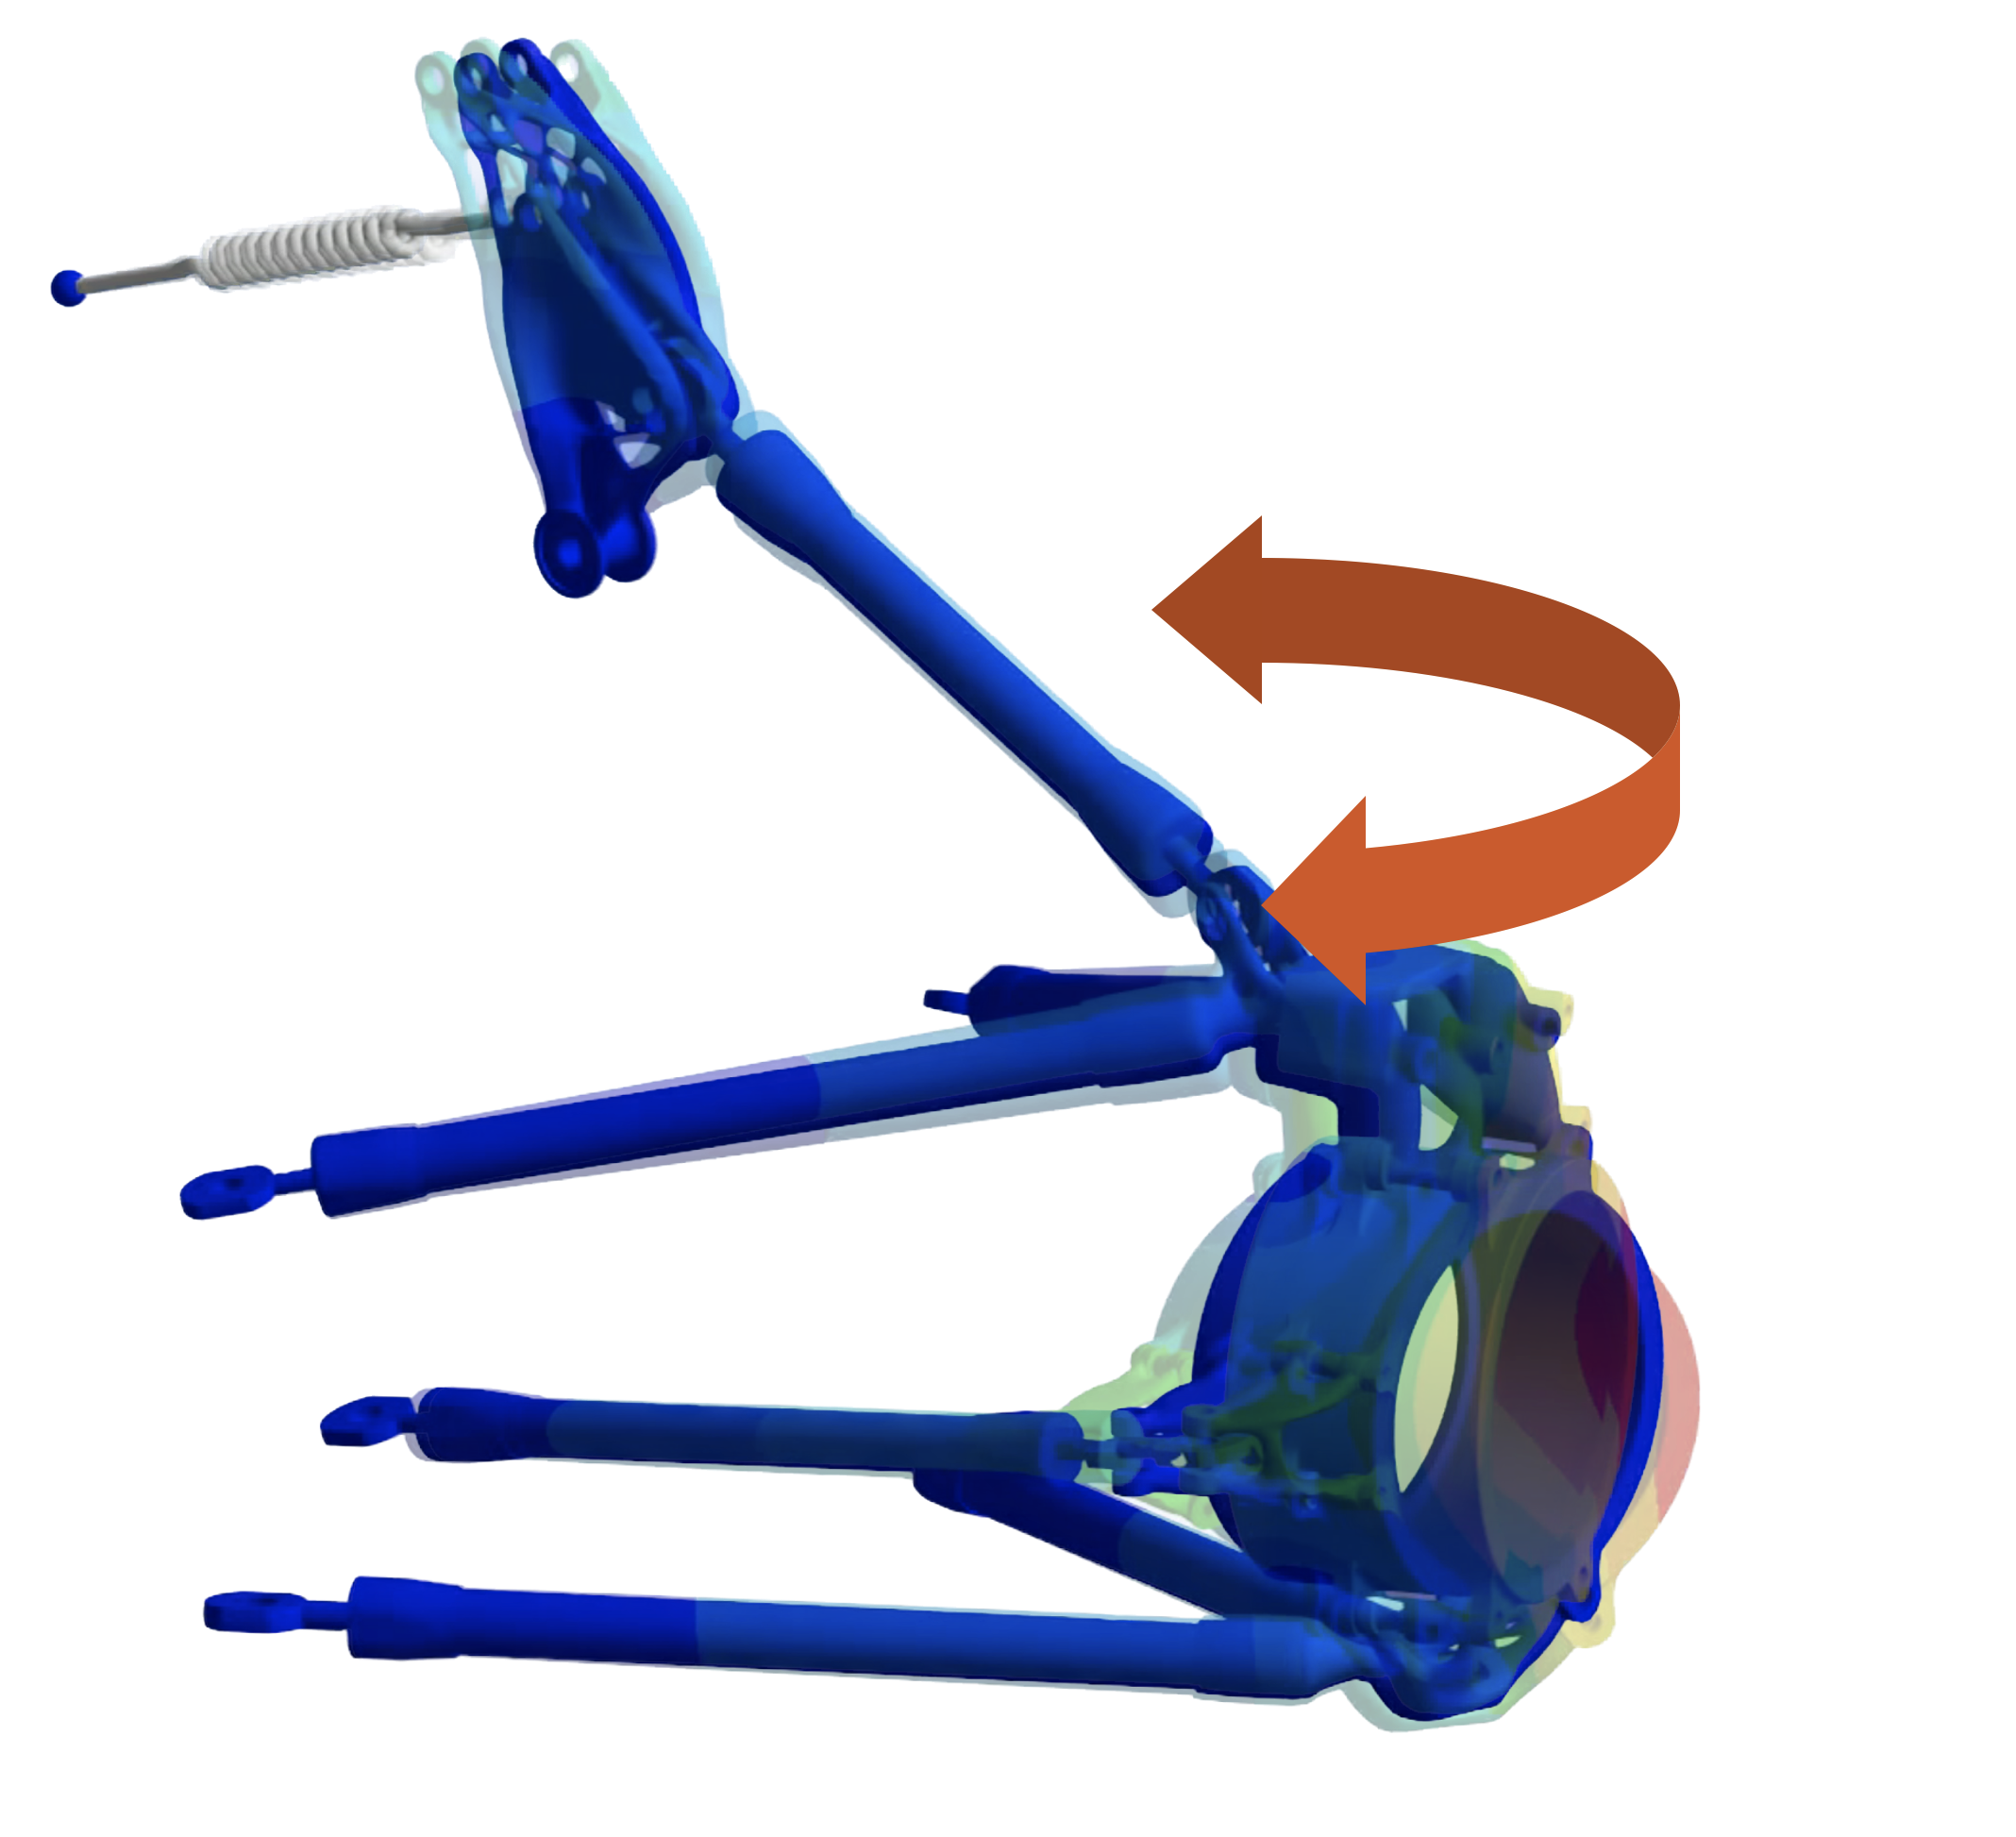
\includegraphics[width=1.0\linewidth]{figures/chapter_4/suspension_mode_2}
    \caption{$f_2 = \SSI{88.5}{\hertz}$}
  \end{subfigure}
  \begin{subfigure}[c]{0.225\textwidth}
    \centering
    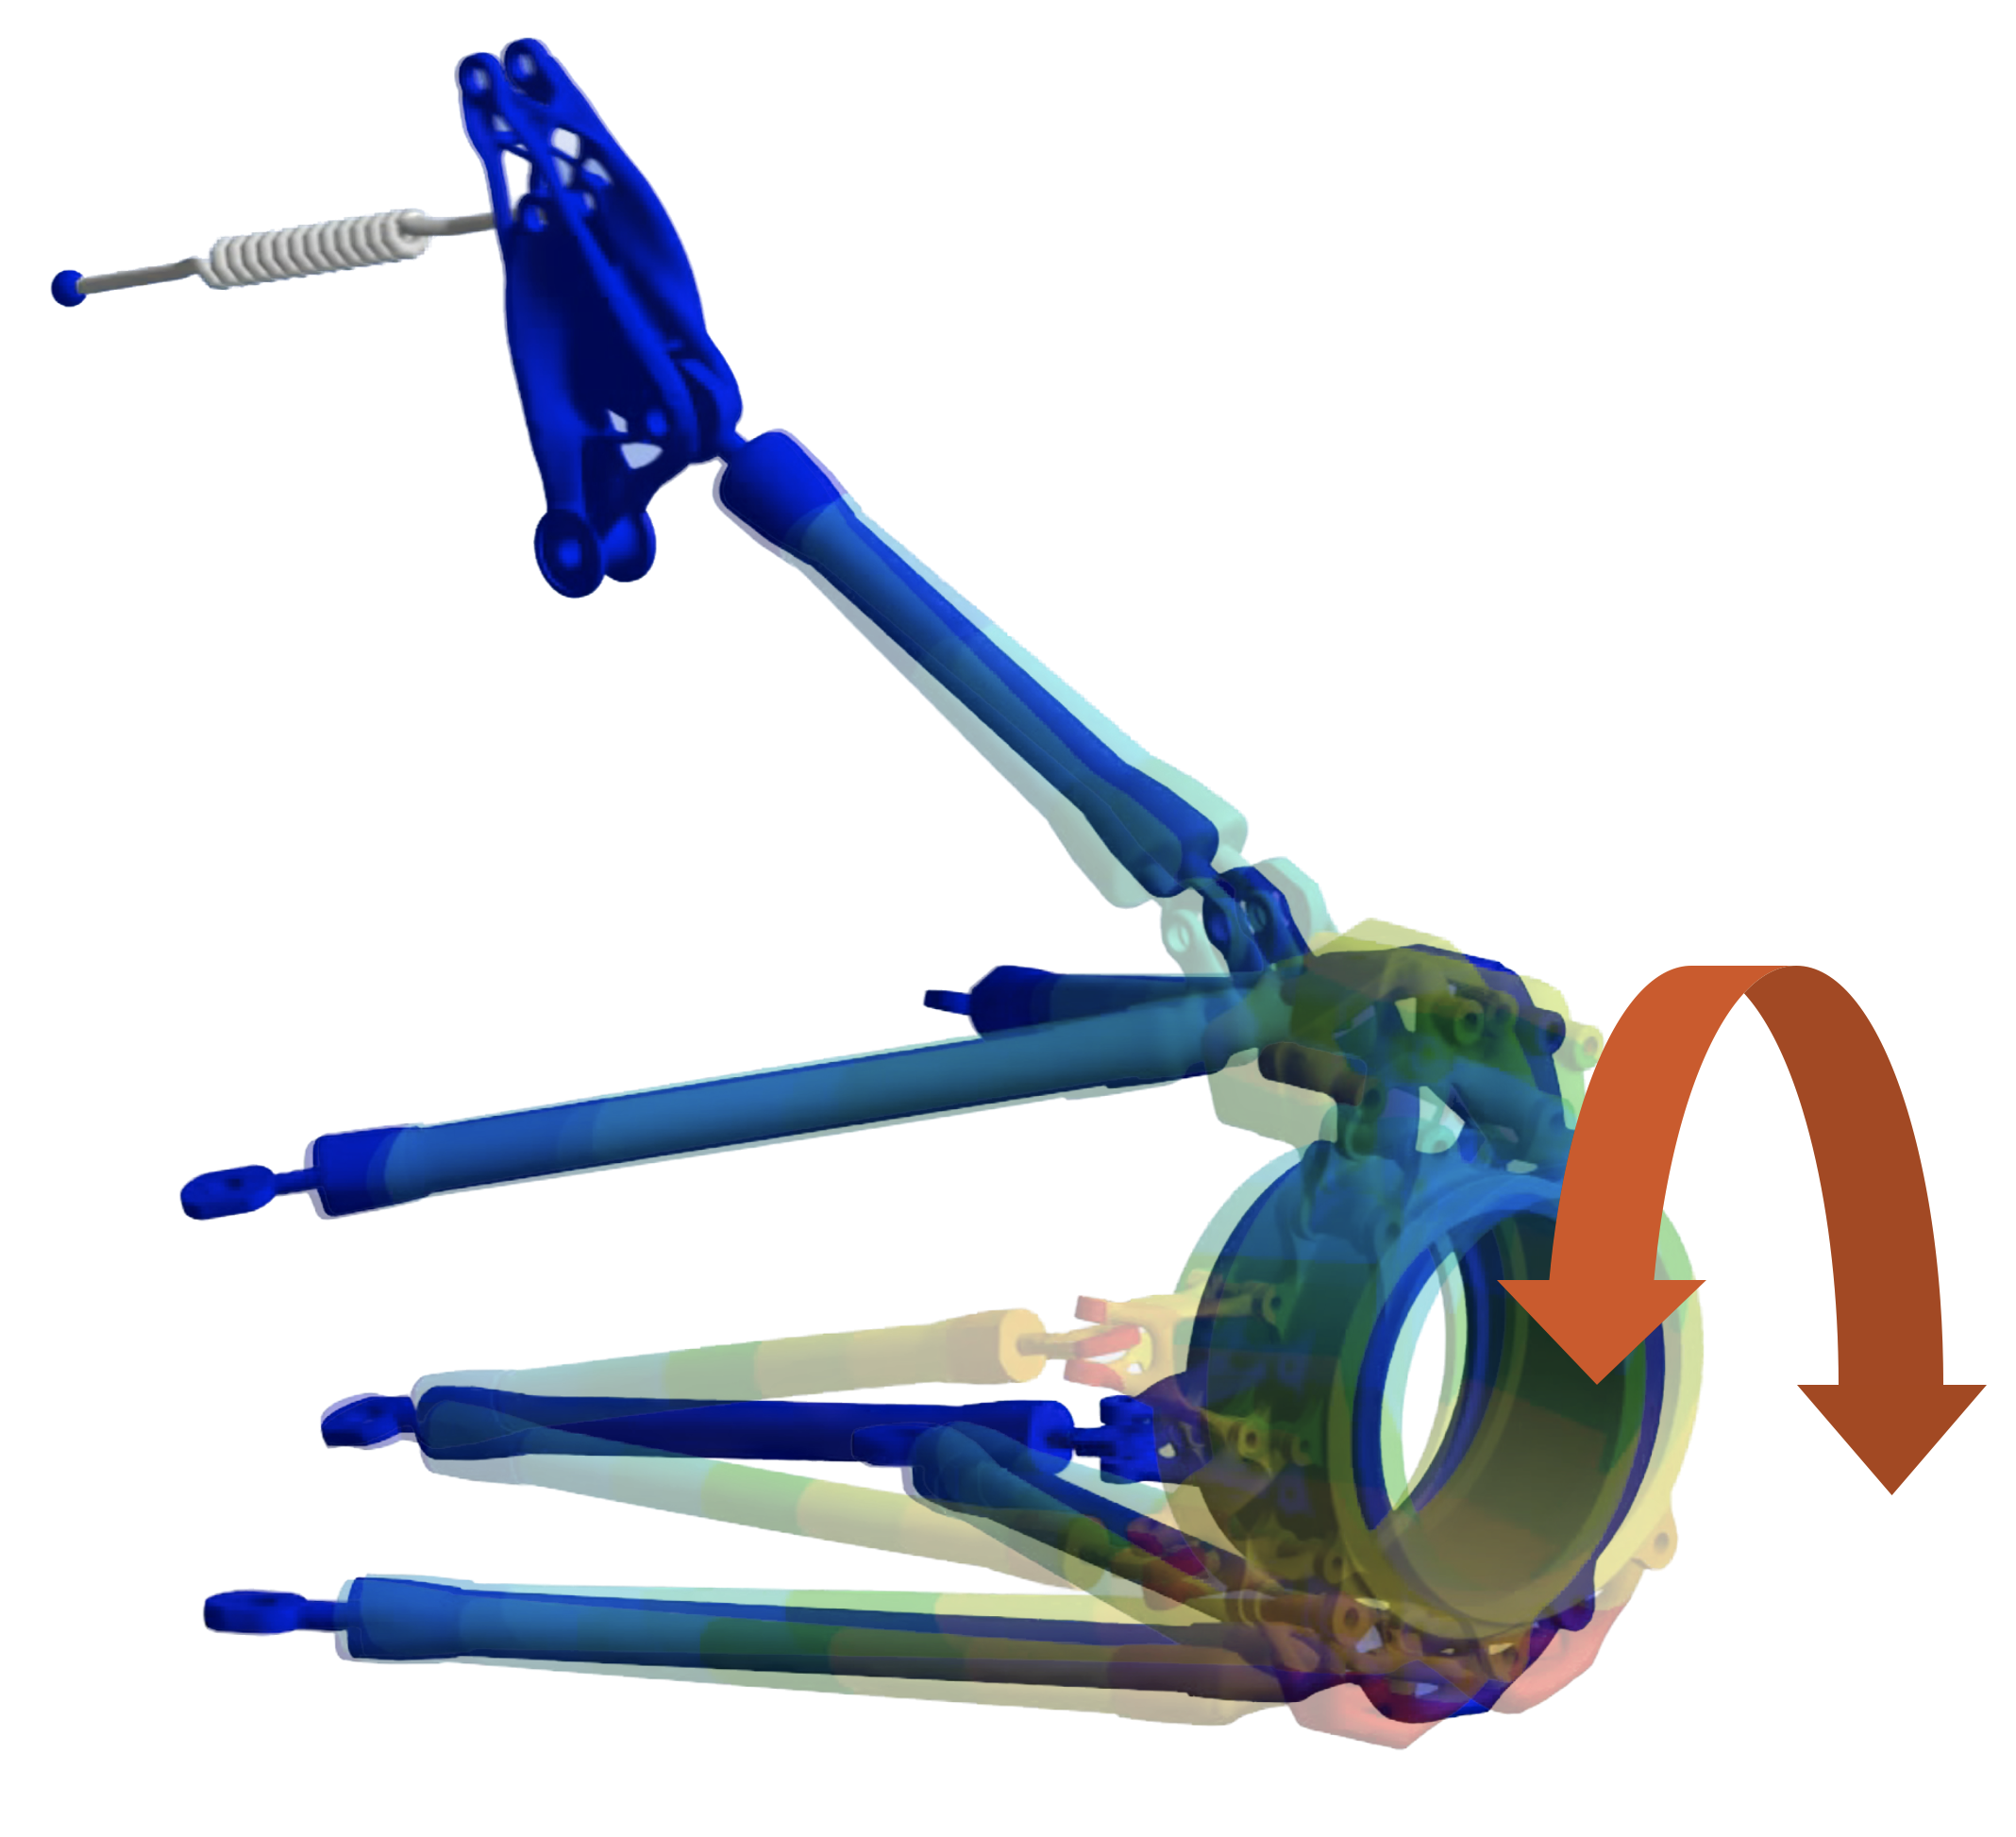
\includegraphics[width=1.0\linewidth]{figures/chapter_4/suspension_mode_3}
    \caption{$f_3 = \SSI{159.7}{\hertz}$}
  \end{subfigure}
  \caption{First three modal shapes of the suspension.}
  \label{chap5:fig:suspension_modes}
\end{figure}

\begin{figure}[htbp]
  \centering
  \small{\includetikz{figures/chapter_4/suspension_dynamic_deformations.tex}}
  \caption{Frequency response analysis of the suspension model is conducted, with tests performed under the equilibrium between the suspension system and a vertical force of \SI{500}{\newton} applied at the wheel hub. Frequency responses are assessed by applying input forces/torques at the wheel hub in the form of a linear chirp spanning frequencies from \SIrange{0}{200}{\hertz}, with a constant amplitude of \SI{5}{\newton}/\SI{5}{\newton\meter}. \emph{Legend:} {\color{mycolor1}$\blacksquare$} \Simulink{} multi-body simulation with full compliance dynamics contribution, {\color{mycolor2}$\blacksquare$} \Simulink{} multi-body with steady-state compliance contribution, {\color{mycolor3}$\blacksquare$} \Ansys{} \ac{FE} modal analysis.}
  \label{chap5:fig:suspension_dynamic_results}
\end{figure}

The reduced system is then used to perform a transient analysis of the suspension system, coupled with the tire-ground enveloping model and the tire model presented in Appendix~\ref{app2:enve} (supported by the \Acme{} \cpp{} library described in Appendix~\ref{app1:acme}) and Appendix~\ref{app3:tirex}, respectively. The transient analysis is conducted to understand the impact of compliance on the vehicle dynamics as well as suspension rods' diameter in the development of tire-ground forces. A side slip angle ramp simulation is thus performed to evaluate the effect of suspension compliance on the lateral force of the tire. For this simulation, the following four cases are analyzed:
%
\begin{itemize}
  \setlength\itemsep{0.0em}
  \item pure kinematic suspension model;
  \item kinematic and nominal compliance model;
  \item kinematic and compliance model with $-10\%$ suspension rods diameter;
  \item kinematic and compliance model with $-20\%$ suspension rods diameter.
\end{itemize}
%
The results of the simulation are shown in Figure~\ref{chap5:fig:test_bench}, which compares the four cases. The lateral force $F_y$ is depicted with solid lines, while the difference between the lateral force of the pure kinematic simulation and the other cases is illustrated in dashed lines. The displayed curves show a non-negligible effect of suspension compliance on the lateral force of the tire is observed. As expected, the larger difference in the generated $F_y$ force can be observed in the linear region of the tire slip characteristic curve, where the slip cornering stiffness is higher. The difference then decreases as the peak approaches. Further observations could be made on the impact of these findings on the vehicle dynamics and handling. However, this is beyond the scope of this work.

\begin{figure}[!htp]
  \centering
  \small{\includetikz{figures/chapter_4//test_bench.tex}}
  \caption{Tire lateral force $F_y$ during a side slip angle ramp simulation. Solid lines represent the results obtained with the \Simulink{} model, while dashed lines represent the difference between the various simulations (see legend below). \emph{Solid lines legend:}
  {\color{mycolor1}\raisebox{-.15pt}{$\blacksquare$}} kinematics, {\color{mycolor2}\raisebox{-.15pt}{$\blacksquare$}} kinematics and compliance, {\color{mycolor3}\raisebox{-.15pt}{$\blacksquare$}} kinematics and compliance ($-10\%$ rods diameter), {\color{mycolor5}\raisebox{-.15pt}{$\blacksquare$}} kinematics and compliance ($-20\%$ rods diameter).   \emph{Dashed lines legend:} {\color{mycolor1}\raisebox{-.15pt}{\scalebox{0.5}[1.0]{$\blacksquare$}}}{\color{mycolor2}\raisebox{-.15pt}{\scalebox{0.5}[1.0]{$\blacksquare$}}} = {\color{mycolor1}\raisebox{-.15pt}{$\blacksquare$}} $-$ {\color{mycolor2}\raisebox{-.15pt}{$\blacksquare$}}, {\color{mycolor1}\raisebox{-.15pt}{\scalebox{0.5}[1.0]{$\blacksquare$}}}{\color{mycolor3}\raisebox{-.15pt}{\scalebox{0.5}[1.0]{$\blacksquare$}}} = {\color{mycolor1}\raisebox{-.15pt}{$\blacksquare$}} $-$ {\color{mycolor3}\raisebox{-.15pt}{$\blacksquare$}},  {\color{mycolor1}\raisebox{-.15pt}{\scalebox{0.5}[1.0]{$\blacksquare$}}}{\color{mycolor5}\raisebox{-.15pt}{\scalebox{0.5}[1.0]{$\blacksquare$}}} = {\color{mycolor1}\raisebox{-.15pt}{$\blacksquare$}} $-$ {\color{mycolor5}\raisebox{-.15pt}{$\blacksquare$}}.
  }
  \label{chap5:fig:test_bench}
\end{figure}

Finally, to estimate what would be the impact of compliance in a racing vehicle, the telemetry and inputs of a full-vehicle simulation conducted on the \textit{Pista Azzurra} track in Jesolo (Italy), are applied to the modeled rear left double wishbone suspension. The simulation is conducted using the previously reduced \ac{MB}-\ac{DAE} system, the tire-ground enveloping model, and the tire model presented in Appendices~\ref{app2:enve} and~\ref{app3:tirex}, respectively. The results of the simulation are shown in Figure~\ref{chap5:fig:suspension_pista_azzurra}, where the suspension travel $z$ is shown in the first plot, while the translations $\delta$ and rotation $\theta$ components of the compliance contribution at the wheel hub are shown in the second and third plots, respectively. The results show that the compliance of the suspension system adds a non-negligible contribution to the wheel hub's positioning, especially in terms of rotations.

\begin{figure}[htbp]
  \centering
  \small{\includetikz{figures/chapter_4/suspension_pista_azzurra.tex}}
  \caption{Simulation of the rear left double wishbone suspension of the Formula SAE \textit{E-Agle Trento Racing Team} vehicle~\cite{eagle} on the \textit{Pista Azzurra} track in Jesolo (Italy). The simulation is conducted using the index-reduced \ac{DAE} system, the tire-ground enveloping model, and the tire model presented in Appendices~\ref{app2:enve} and~\ref{app3:tirex}, respectively. In the first plot, the suspension travel $z$ is shown, while the second and third plots show the translations $\delta$ and rotation $\theta$ components of the compliance contribution at the wheel hub. \emph{Legend}: {\color{mycolor1}$\blacksquare$} $x$-axis component, {\color{mycolor2}$\blacksquare$} $y$-axis component, {\color{mycolor3}$\blacksquare$} $z$-axis component.}
  \label{chap5:fig:suspension_pista_azzurra}
\end{figure}

\section{Trajectory Prescribed Path Control}
\label{chap5:sec:tppc}

The \ac{TPPC} category is characterized by \ac{DAE} systems that describe the motion of a dynamical system whose trajectory is prescribed by adding a set of path constraints to the equations of motion. The model equations evolve into a non-linear semi-explicit \acp{DAE}. Within this system, the differential equations represent motion equations, while the algebraic equations correspond to imposed path constraints, collectively constituting \ac{TPPC} problems. Historically, addressing specific \ac{TPPC} challenges involved the development of software models that promptly adjust control variables to approximate prescribed path profiles. In this context, we investigate general numerical techniques directly applicable to \acp{DAE}. \ac{TPPC} problems are present in various fields, such as robot control, chemical process management, as well as space vehicle and aircraft guidance.

The \ac{DAE} systems arising from \ac{TPPC} simulations has typically the Hessenberg form~\cite{brenan1986numerical}
%
\begin{equation*}
  \begin{cases}
    \m{x}^\prime = \m{f}(\m{x}, \m{u}, t) & \text{differential equations} \\
    \m{0}        = \m{g}(\m{x}, \m{u}, t) & \text{path constraints}
  \end{cases} \, \text{,}
  \quad \text{with} \quad \jac{\m{g}}{\m{x}} \, \jac{\m{f}}{\m{u}} ~ \text{non-singular}
  \label{chap5:eq:tppc_dae_index2}
\end{equation*}
%
for index-2 problems, and
%
\begin{equation*}
  \begin{cases}
    \m{x}^\prime = \m{f}(\m{x}, \m{y}, \m{u}, t) \\
    \m{y}^\prime = \m{g}(\m{x}, \m{y}, t) \\
    \m{0}        = \m{h}(\m{y}, t)
  \end{cases} \, \text{,}
  \quad \text{with} \quad \jac{\m{h}}{\m{y}} \, \jac{\m{g}}{\m{x}} \, \jac{\m{f}}{\m{u}} ~ \text{non-singular}
  \label{chap5:eq:tppc_dae_index3}
\end{equation*}
%
for index-3 problems. The index of such systems is typically higher than the non-controlled counterpart. Indeed, the path constraints control is embedded in the state equations, often increasing the length of the differentiation chain to obtain a set of \acp{ODE}. Specifically, when the Jacobian $\jac{\m{g}}{\m{u}}$ is non-singular, the path equations are commonly referred to as control variable constraints and the corresponding \acp{DAE} has index-1. It is not uncommon to find that the path constraints in a \ac{TPPC} problem are functions only of the differential variables so that $\jac{\m{g}}{\m{u}} = \m{0}$ and the \acp{DAE} will be of higher index~\cite{brenan1995numerical}. To showcase the capabilities of the proposed index reduction algorithm in handling such high-index \ac{TPPC} problems, different examples are presented. Two problems regarding the initial and final phases of the space shuttle reentry, described by index-2 and index-3 \acp{DAE}~\cite{brenan1995numerical}. Lastly, one problem on the control of a robotic arm, which is described as a complicated index-5 system~\cite{pryce1998solving}. A brief discussion of each of these examples, together with an introduction to the application field, is presented in the following sections.

\subsection{Space Shuttle Reentry Problems}

In space applications, \ac{TPPC} problems aid in vehicle performance analysis during design, particularly for lifting reentry vehicles aiming to determine maximum crossrange (or downrange) capability. Trajectory profiles are constrained by skin temperature limits set by the thermal protection design. \ac{OC} theory offers a direct approach to addressing maximum crossrange capability with heating constraints, formulated as a two-point boundary value problem involving \acp{DAE} and adjoint variables. However, solving such \acp{OCP} requires starting solutions close to the optimal, especially with heating constraints, due to extreme sensitivity to initial guesses in shooting problems. An indirect \ac{TPPC} approach or using \ac{TPPC} to generate initial solutions for \ac{OC} may offer more success. Typically, maximizing crossrange capability involves holding the angle of attack $\alpha$ near the maximum lift/drag value, often set at around \SI{40}{\deg} in \ac{NASA} space shuttle reentry simulations, leaving bank angle $\beta$ adjustments to satisfy remaining functional constraints. In certain scenarios, varying system parameters can effectively optimize vehicle crossrange capability by ensuring trajectory adherence to specific constraints, thereby presenting a semi-explicit non-linear \acp{DAE} \ac{TPPC} problem~\cite{brenan1986numerical, brenan1995numerical}.

The discussion is confined to a reentry vehicle in the absence of propulsive forces, where we simplify the simulation to model solely spherical geopotential and spherical earth. The equations of motion in relative coordinates are thus expressed as follows
%
\begin{equation}
  \begin{cases}
  H^{\prime}       = V_r\sin(\gamma) \\
  \xi^{\prime}     = \dfrac{V_r\cos(\gamma) \sin(A)}{r \cos(\lambda)} \\
  \lambda^{\prime} = \dfrac{V_r}{r} \cos(\gamma) \cos(A) \\
  V_r^{\prime}     = -\dfrac{D}{m} - g\sin(\gamma) - \Omega_e^2 r \cos(\lambda)(\sin(\lambda) \cos(A) \cos(\gamma)-\cos(\lambda) \sin(\gamma)) \\
  \gamma^{\prime}  = \dfrac{L\cos(\beta)}{m V_r}+\dfrac{\cos(\gamma)}{V_r}\left(\dfrac{V_r^2}{r}-g\right) + 2\Omega_e \cos(\lambda) \sin(A)\dots \\
  \qquad + \dfrac{\Omega_e^2 r \cos(\lambda)}{V_r}(\sin(\lambda) \cos(A) \sin(\gamma)+\cos(\lambda) \cos(\gamma)) \\
  A^{\prime}       = \dfrac{L\sin(\beta)}{m V_r \cos(\gamma)}+\dfrac{V_r}{r} \cos(\gamma) \sin(A) \tan(\lambda) - 2\Omega_e(\cos(\lambda) \cos(A) \tan(\gamma) - \sin(\lambda)) \dots \\
  \qquad + \dfrac{\Omega_e^2 r \cos(\lambda) \sin(\lambda) \sin(A)}{V_r \cos(\gamma)}
  \end{cases} \, \text{,}
  \label{chap5:eq:space_shuttle_reentry}
\end{equation}
%
where the state variables are $\m{x} = [H, \xi, \lambda, V_r, \gamma, A]^\top$. The parameters are the following
%
\begin{equation*}
  \begin{aligned}
    r           & = H + r_e, & \text{distance from the earth center,} \\
    r_e         & = \SI{20902900}{\feet} & \text{earth radius,} \\
    g           & = \mu/r^2 & \text{gravity force,} \\
    \mu         & = \SI{1.407653916\times 10^16}{\cubic\feet\per\second\squared} & \text{gravitational constant,} \\
    \Omega_e    & = \SI{360/(24\cdot60\cdot60)}{\deg\per\second} & \text{earth angular speed,} \\
    \rho(H)     & = 0.002378\exp(-H/23800) & \text{atmospheric density,} \\
    L(V_r)      & = 1/2 \rho C_L S V_r^2 & \text{aerodynamic lift force,} \\
    D(V_r)      & = 1/2 \rho C_D S V_r^2 & \text{aerodynamic drag force.}
  \end{aligned}
\end{equation*}
%
The aerodynamic lift and drag coefficients, respectively $C_L(\alpha)$ and $C_D(\alpha)$, as well as the vehicle cross-sectional area $S$ and mass $m$, will be later specified on the specific test. The control variables, which dictate both the magnitude and direction of the aerodynamic force applied to the vehicle, are assessed within the body coordinate system (refer to Figure~\ref{chap5:fig:shuttle_frame}). The bank angle $\beta$ corresponds to a rotation or \emph{roll} about the vehicle's $x$-axis, while the angle of attack $\alpha$ is measured from the relative velocity vector of the vehicle to the body $x$-axis, representing a rotation or \emph{pitch} about the body $y$-axis. For a more detailed explanation of these parameters and the coordinate system on the presented tests, please refer to~\cite{brenan1983stability}. Nonetheless, figure~\ref{chap5:fig:shuttle_reentry} illustrates the space shuttle coordinate system, as well as the vehicle's position with respect to the earth reference frame.

\begin{figure}[htb]
  \centering
  \begin{subfigure}[c]{0.475\textwidth}
    \centering
    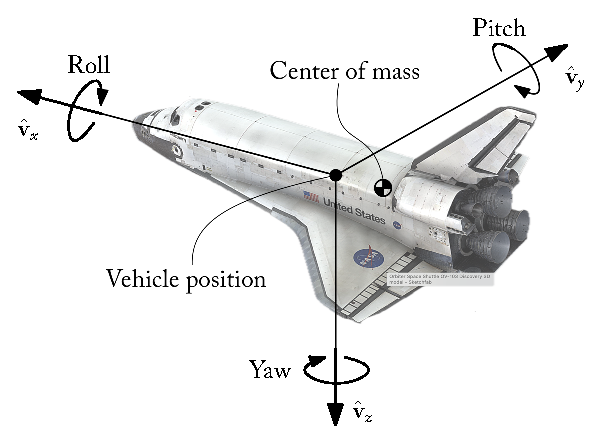
\includegraphics[width=1.0\linewidth]{figures/chapter_4/shuttle_frame.eps}
    \caption{Space shuttle reentry vehicle coordinate system.}
    \label{chap5:fig:shuttle_frame}
  \end{subfigure}%
  \hfill
  \begin{subfigure}[c]{0.475\textwidth}
    \centering
    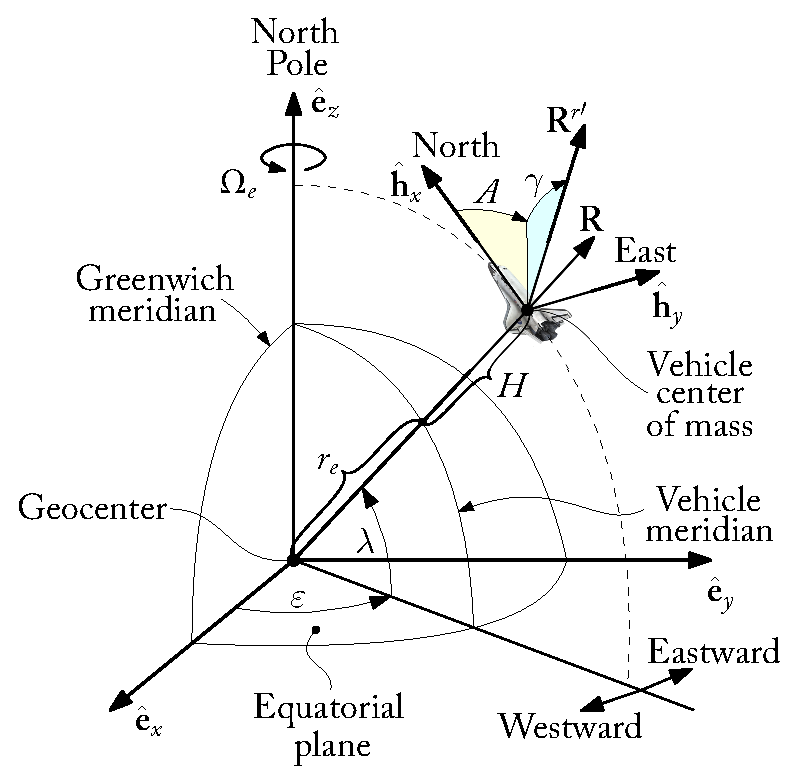
\includegraphics[width=1.0\linewidth]{figures/chapter_4/earth_frame.eps}
    \caption{Earth reference frame.}
    \label{chap5:fig:earth_frame}
  \end{subfigure}
  \caption{Coordinate systems for the space shuttle reentry problem~\cite{brenan1995numerical, brenan1986numerical}.}
  \label{chap5:fig:shuttle_reentry}
\end{figure}

Once the space shuttle concludes its mission in space, it must return to Earth for landing, subject to various mission constraints, such as heating limitations to prevent vehicle damage. Instead of directly imposing these heating constraints as algebraic limitations, an alternative approach involves prescribing a nominal drag acceleration versus a relative velocity profile. This profile is selected to ensure that temperature constraints are satisfied as long as the vehicle follows a trajectory complying with this drag constraint. During reentry, the standard equations of motion~\eqref{chap5:eq:space_shuttle_reentry} are compounded with an algebraic constraint representing the drag acceleration profile, forming a \ac{DAE} system. Typically, the angle of attack remains constant or is only slightly varied, while the bank angle serves as the control variable. In the following, we examine the initial and final phases of reentry. The first involves maneuvering the vehicle from a given state to one lying on the nominal drag constraint. While the second entails flying the vehicle along the nominal drag constraint.

\subsubsection{Initial Stage Reentry Problem}

We now examine the initial stage reentry \ac{TPPC} problem in the same form of~\cite{brenan1986numerical}. This problem is part of a broader trajectory optimization process aimed at determining a surface of admissible reentry states. Following completion of on-orbit maneuvers, the vehicle must transition to a state vector enabling safe flight to the landing site. This set of allowable states is denoted as a target line. A given initial state qualifies as a target line point if a trajectory can be executed from that state in such a way that the vehicle's drag versus relative velocity profile smoothly aligns with the specified nominal profile, without overshooting and thus without violating any temperature constraints. Consider now the description of the vehicle's drag acceleration versus relative velocity profile, expressed as
%
\begin{equation}
  \dfrac{D}{m} - (C_0 + C_1 (V_r - V_0) + C_2 (V_r - V_0)^2 + C_3 (V_r - V_0)^3) = 0 \, \text{,}
  \label{chap5:eq:initial_drag}
\end{equation}
%
for a time $t \in [t_0, t_1] = \RSI{32.868734542}{419.868734542}{\second}$, and where $V_0$, is the vehicle's initial velocity at $t_0$ and $C_0 = 3.974960446019$, $C_1 = -0.01448947694635$, $C_2 = -0.2156171551995 \cdot 10^{-4}$, and $C_3 = -0.1089609507291 \cdot 10^{-7}$ are constants chosen so that the initial state vector satisfies~\eqref{chap5:eq:initial_drag} and its first derivative at $t_0$, and so that this transitional phase smoothly joins with the nominal profile. Notice that, posed in this way, the resulting \ac{TPPC} system is a semi-explicit index-3 \acp{DAE} problem. In this test, the set of initial values are $\gamma = \SI{-0.749986488}{\deg}$, $A = \SI{62.7883367}{\deg}$, $H = \SI{264039.3280}{\feet}$, $\xi = \SI{177.718047}{\deg}$, $\lambda = \SI{32.0417885}{\deg}$, $V_r = \SI{24317.0798}{\feet\per\second}$, and $\beta = \SI{41.10071834}{\deg}$. The lift and drag coefficients $C_L = 0.8769230769$ and $C_D = 0.8246153846$, as well as the angle of attack $\alpha = \SI{40}{\deg}$ are assumed to be constant throughout the simulation. The vehicle mass is $m = \SI{5964.496499824}{\slugs}$, and its cross-sectional reference area is $S = \SI{2690}{\feet\squared}$.

\begin{table}
  \caption{Expression complexity encountered throughout the index reduction of the initial stage space shuttle reentry problem~\cite{brenan1995numerical} \ac{DAE} system. \emph{Legend}: $\cf$ = functions, $\ca$ = additions, $\cm$ = multiplications, and $\cd$ = divisions.}
  \label{chap5:tab:tppc_initial}
  \centering
  {\footnotesize\begin{tabular}{cccc}
    \multicolumn{4}{c}{\textbf{Initial Stage Space Shuttle Reentry Problem~\cite{brenan1995numerical}}} \\
    \toprule
    \textbf{Original \acp{DAE}} & \multicolumn{3}{c}{$\mF = 153\cf + 2\cd + 275\cm + 59\ca$ \quad $\mh = 0$} \\
    \midrule
    \textbf{Reduction step} & $\mE$ & $\mg$ & $\ma$ \\
    \midrule
    Index-3 \acp{DAE} & $11\cf + 9\cm + 5\ca$ & $118\cf + 1\cd + 220\cm + 36\ca$ & $6\cf + 1\cd + 28\cm + 10\ca$ \\
    Index-2 \acp{DAE} & $11\cf + 9\cm + 5\ca$ & $118\cf + 1\cd + 220\cm + 36\ca$ & $81\cf + 2\cd + 472\cm + 87\ca$ \\
    Index-1 \acp{DAE} & $11\cf + 9\cm + 5\ca$ & $118\cf + 1\cd + 220\cm + 36\ca$ & $567\cf + 3\cd + 6198\cm + 888\ca$ \\
    Index-0 \acp{DAE} & $4053\cf + 24\cd + 41102\cm + 5792\ca$ & $118\cf + 1\cd + 220\cm + 36\ca$ & $0$ \\
    \midrule
    \textbf{Reduced \acp{DAE}} & \multicolumn{3}{c}{$\mF = 3075\cf + 4\cd + 34811\cm + 4734\ca$ \quad $\mh = 654\cf + 6\cd + 6698\cm + 985\ca$} \\
    \bottomrule
  \end{tabular}}
\end{table}

To address this index-3 \acp{DAE}, we utilize the proposed index reduction algorithm. The complexity of expressions encountered during the algorithm's execution is detailed in Table~\ref{chap5:tab:tppc_initial}. Notably, the index reduction algorithm effectively reduced the system to index-0 without the aid of hierarchical representations, and the expression growth is strongly inhibited by successful simplification and only limited to the last reduction step. We conduct numerical integration of the reduced \ac{DAE} system using both the \Maple{} and \Indigo{} solvers. Specifically, \Maple{} encounters challenges in integrating the original \ac{DAE} system due to difficulties in projecting initial values into the solution space, where \acp{IC} are deemed inconsistent with the algebraic constraints. In contrast, the \Indigo{} numerical solver successfully integrates the reduced \ac{DAE} system, yielding results depicted in Figure~\ref{chap5:fig:tppc_initial}.

\begin{figure}[htb]
  \centering
  \small{\includetikz{figures/chapter_4/shuttle_index3_control.tex}}
  \caption{Control history of the initial stage space shuttle reentry problem~\cite{brenan1995numerical}. The vehicle's trajectory is prescribed by the drag acceleration $D/m$ versus a relative velocity $V_r$ profile reported in~\eqref{chap5:eq:initial_drag}. The vehicle's state is controlled by the bank angle $\beta$ and the angle of attack is kept fixed at $\alpha = \SI{40}{\deg}$. \emph{Legend}: \textcolor{mycolor1}{$\blacksquare$} bank angle $\beta$, and \textcolor{mycolor2}{$\blacksquare$} angle of attack $\alpha$.}
  \label{chap5:fig:tppc_initial}
\end{figure}

\subsubsection{Final Stage Reentry Problem}

We now examine the final stage reentry \ac{TPPC} problem in the same form of~\cite{brenan1995numerical}. Let us assume the objective is to navigate a vehicle along a predetermined azimuth $A$ and flight path angle trajectory $\gamma$, as defined by the constraints on state variables
%
\begin{equation}
  \gamma + 1 + 9\left(\dfrac{t}{300}\right)^2 = 0 \, \text{,}
  \qquad \text{and} \qquad
  A - 45 + 90\left(\dfrac{t}{300}\right)^2 = 0 \, \text{.}
  \label{chap5:eq:final_path_constraints}
\end{equation}
%
for a time $t \in \RSI{0}{300}{\second}$. The flight path angle $\gamma$ spans from $\RSI{-1}{-10}{\deg}$, while the azimuth $A$ ranges from $\RSI{45}{135}{\deg}$. Both the bank angle $\beta$ and the angle of attack $\alpha$ serve as control variables, \ie{} $\m{u} = [\beta, \alpha]^\top$. The \ac{DAE} system is index-2 for a lifting reentry vehicle as long as $(0.05 \rho S V_r/m)^2 C_L(\alpha)/\cos(\gamma) \neq 0$. Notice that to be physically consistent we require that $V_r \neq \SI{0}{\deg}$, $\rho\neq \SI{0}{\deg}$, $\alpha \neq \SI{0}{\deg}$, $\gamma \neq \SI{90}{\deg}$, as well as $\lambda \neq \SI{180}{\deg}$. The related index-1 \acp{DAE} can be obtained directly by differentiating the algebraic constraints once and substituting for $A^\prime$ and $\gamma^\prime$ from the differential equations. Consistent initial values for the \ac{DAE} system are determined by selecting the initial differential and control variables to satisfy~\eqref{chap5:eq:final_path_constraints} the two new hidden constraints in the related index-1 system. The set of initial values used in this experiment are $H = \SI{100000}{\feet}$, $\xi = \SI{0}{\deg}$, $\lambda = \SI{0}{\deg}$, $A = \SI{0}{\deg}$, $V_r = \SI{12000}{\feet\per\second}$, $\gamma = \SI{-1}{\deg}$, $A = \SI{45}{\deg}$, $\beta = \SI{-0.05220958616134}{\deg}$, and $\alpha = \SI{2.6728700742}{\deg}$. The lift and drag coefficients are set to $C_L = 0.01\alpha$ and $C_D = 0.04 + 0.1C_L^2$, respectively. The vehicle mass is $m = \SI{2.890532728}{\slugs}$, and its cross-sectional reference area is $S = \SI{1}{\feet\squared}$.

\begin{table}
  \caption{Expression complexity encountered throughout the index reduction of the final stage space shuttle reentry problem~\cite{brenan1995numerical} \ac{DAE} system. \emph{Legend}: $\cf$ = functions, $\ca$ = additions, $\cm$ = multiplications, and $\cd$ = divisions.}
  \label{chap5:tab:tppc_final}
  \centering
  {\footnotesize\begin{tabular}{cccc}
    \multicolumn{4}{c}{\textbf{Final Stage Space Shuttle Reentry Problem~\cite{brenan1995numerical}}} \\
    \toprule
    \textbf{Original \acp{DAE}} & \multicolumn{3}{c}{$\mF = 157\cf + 1\cd + 272\cm + 56\ca$ \quad $\mh = 0$} \\
    \midrule
    \textbf{Reduction step} & $\mE$ & $\mg$ & $\ma$ \\
    \midrule
    Index-2 \acp{DAE} & $11\cf + 9\cm + 5\ca$ & $126\cf + 1\cd + 237\cm + 39\ca$ & $2\cf + 4\cm + 4\ca$ \\
    Index-1 \acp{DAE} & $5\cf + 3\cm + 3\ca$ & $43\cf + 89\cm + 14\ca$ & $92\cf + 1\cd + 173\cm + 30\ca$ \\
    Index-0 \acp{DAE} & $428\cf + 6\cd + 714\cm + 119\ca$ & $52\cf + 1\cd + 107\cm + 18\ca$ & $0$ \\
    \midrule
    \textbf{Reduced \acp{DAE}} & \multicolumn{3}{c}{$\mF = 425\cf + 1\cd + 742\cm + 138\ca$ \quad $\mh = 94\cf + 1\cd + 177\cm + 34\ca$} \\
    \bottomrule
  \end{tabular}}
\end{table}

To solve the index-2 \ac{DAE} system, we apply the proposed index reduction algorithm. The expression complexity encountered throughout the index reduction is reported in Table~\ref{chap5:tab:tppc_final}. As we can see, the index reduction algorithm successfully reduces the index of the \ac{DAE} system to index-0 with minimal expression swelling in the last reduction step. The numerical integration of the reduced \ac{DAE} system is performed using both the \Maple{} and \Indigo{} numerical solvers. In this regard, \Maple{} is again not able to integrate the original \ac{DAE} system due to the incapacity of projecting the initial values into the solution space (\ie{}, \acp{IC} are not judged to be consistent with the algebraic constraints). Conversely, the numerical integration of the reduced \ac{DAE} system using the \Indigo{} numerical solver is successful, and the results are presented in Figure~\ref{chap5:fig:tppc_final}, where the bank angle $\beta$ and the angle of attack $\alpha$ controls history are shown.

\begin{figure}[htb]
  \centering
  \small{\includetikz{figures/chapter_4/shuttle_index2_control.tex}}
  \caption{Controls history of the space shuttle reentry problem~\cite{brenan1995numerical} in the time interval $t \in \RSI{0}{300}{\second}$. \emph{Legend}: \textcolor{mycolor1}{$\blacksquare$} bank angle $\beta$, and \textcolor{mycolor2}{$\blacksquare$} angle of attack $\alpha$.}
  \label{chap5:fig:tppc_final}
\end{figure}

\subsection{Robot Arm Control}

Another example of a \ac{TPPC} problem is the control of a robot arm, described as an index-5 \ac{DAE} system~\cite{pryce1998solving}. The system describes the path control of a two-link, flexible joint, planar robotic arm from~\cite{campbell1988general}. This system, which is frequently used as a \acp{DAE} benchmark test, is characterized by a high index -- typical of \ac{TPPC} problems -- as well as by the presence of various singularities~\cite{schwarz2020singularities}. The problem is a semi-explicit \acp{DAE} of dimension 8 with 2 path constraints. The system is described by the following equations
%
\begin{equation}
  \begin{cases}
    x_1^{\prime} = x_4 \\
    x_2^{\prime} = x_5 \\
    x_3^{\prime} = x_6 \\
    x_4^{\prime} = 2c(x_3)(x_4+x_6)^2 - x_4^2d(x_3) - (2x_3-x_2)(a(x_3)+2b(x_3)) - a(x_3)(u_1-u_2) \\
    x_5^{\prime} = 2c(x_3)(x_4+x_6)^2 - x_4^2d(x_3) + (2 x_3-x_2)(1-3a(x_3)-2b(x_3)) - a(x_3)(u_1-u_2) + u_2 \\
    x_6^{\prime} = 2c(x_3)(x_4+x_6)^2 - x_4^2d(x_3) + (2 x_3-x_2)(a(x_3)-9b(x_3)) - (a(x_3)+b(x_3))(u_1-u_2) \dots \\
    \qquad - d(x_3)(x_4+x_6)^2 - 2x_4^2c(x_3) \\
    0 = \cos(x_1) + \cos(x_1+x_3) - p_1(t) \\
    0 = \sin(x_1) + \sin(x_1+x_3) - p_2(t)
  \end{cases} \, \text{,}
\end{equation}
%
with
%
\begin{equation}
  a(z) = \dfrac{2}{2-\cos(z)^2} \, \text{,}
  \quad
  b(z) = \dfrac{\cos(z)}{2-\cos(z)^2} \, \text{,}
  \quad
  c(z) = \dfrac{\sin(z)}{2-\cos(z)^2} \, \text{,}
  \quad \text{and} \quad
  d(z) = \dfrac{\cos(z)\sin(z)}{2-\cos(z)^2} \, \text{.}
\end{equation}
%
Here, the variables $[x_1, x_2, x_3]$ represent the angular coordinates of the end effector, while $[x_4, x_5, x_6]$ are their derivatives. The control variables are $[u_1, u_2]$, which represent the torques applied to the joints. The end effector path constraints are given by
%
\begin{equation}
  p_1(t) = \cos(\exp(t) - 1) + \cos(t - 1) \, \text{,}
  \quad \text{and} \quad
  p_2(t) = \sin(1 - \exp(t)) + \sin(1 - t) \, \text{.}
\end{equation}
%
Figure~\ref{chap5:fig:robotic_arm} illustrates the robotic arm problem, as well as its variables and control parameters.

\begin{figure}[htb]
  \centering
  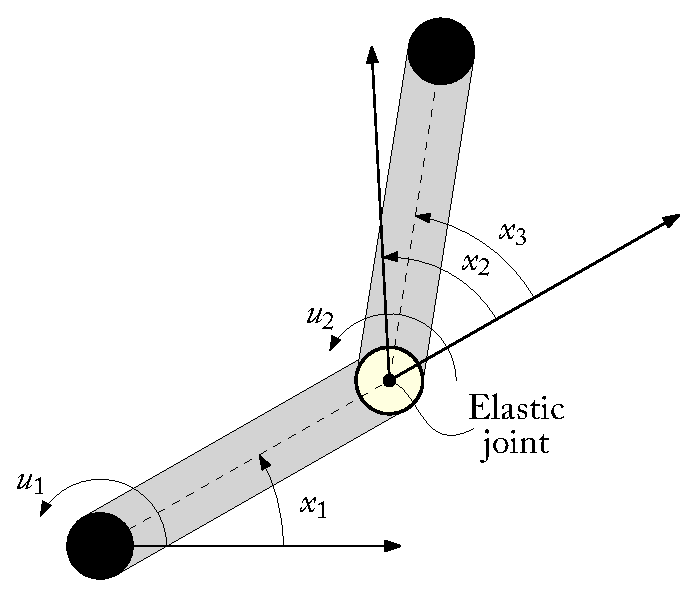
\includegraphics[width=0.4\linewidth]{figures/chapter_4/robotic_arm.eps}
  \caption{Robot arm control problem.}
  \label{chap5:fig:robotic_arm}
\end{figure}

\begin{table}
  \caption{Expression complexity encountered throughout the index reduction of the robotic arm problem~\cite{brenan1995numerical} \ac{DAE} system. \emph{Legend}: $\cf$ = functions, $\ca$ = additions, $\cm$ = multiplications, and $\cd$ = divisions.}
  \label{chap5:tab:tppc_robot}
  \centering
  \resizebox{\textwidth}{!}{%
  {\footnotesize\begin{tabular}{cccc}
    \multicolumn{4}{c}{\textbf{Robotic Arm~\cite{pryce1998solving}}} \\
    \toprule
    \textbf{Original \acp{DAE}} & \multicolumn{3}{c}{$\mF = 125\cf + 19\cd + 56\cm + 64\ca$ \quad $\mh = 0$} \\
    \midrule
    \textbf{Reduction step} & $\mE$ & $\mg$ & $\ma$ \\
    \midrule
    Index-5 \acp{DAE} & $0$ & $66\cf + 3\cd + 50\cm + 35\ca$ & $16\cf + 12\ca$ \\
    Index-4 \acp{DAE} & $0$ & $66\cf + 3\cd + 50\cm + 35\ca$ & $24\cf + 6\cm + 14\ca$ \\
    Index-3 \acp{DAE} & $0$ & $66\cf + 3\cd + 50\cm + 35\ca$ & $162\cf + 2\cd + 138\cm + 114\ca$ \\
    Index-2 \acp{DAE} & $14\cf + 2\cd + 6\cm + 6\ca$ & $372\cf + 4\cd + 375\cm + 253\ca$ & $972\cf + 1\cd + 1062\cm + 770\ca$ \\
    Index-1 \acp{DAE} & $14\cf + 2\cd + 6\cm + 6\ca$ & $372\cf + 4\cd + 375\cm + 253\ca$ & $\star (6.5\cf + 5.6\cm + 1.8\ca)\cdot10^{6} + 4\cd$ \\
    Index-0 \acp{DAE} & $\star (8.3\cf + 7.1\cm + 2.3\ca)\cdot10^{7} + 58\cd$ & $(2.4\cf + 2.0\cm + 0.9\ca)\cdot10^{6} + 8\cd$ & $0$ \\
    \midrule
    \textbf{Reduced \acp{DAE}} & \multicolumn{3}{c}{$\star \mF = (8.6\cf + 7.3\cm + 2.4\ca)\cdot10^{7} + 66\cd$ \quad $\star \mh = (6.5\cf + 5.6\cm + 1.8\ca)\cdot10^{6} + 7\cd$} \\
    \bottomrule
    \end{tabular}}
    }
\end{table}

\begin{table}
  \caption{Expression complexity encountered throughout the index reduction with the aid of hierarchical representation of the robotic arm problem~\cite{brenan1995numerical} \ac{DAE} system. \emph{Legend}: $\cf$ = functions, $\cv$ = veiling variables, $\ca$ = additions, $\cm$ = multiplications, and $\cd$ = divisions.}
  \label{chap5:tab:tppc_robot_veil}
  \centering
  {\footnotesize\begin{tabular}{cccc}
    \multicolumn{4}{c}{\textbf{Robotic Arm~\cite{pryce1998solving}}} \\
    \toprule
    \textbf{Original \acp{DAE}} & \multicolumn{3}{c}{$\mF = 125\cf + 19\cd + 56\cm + 64\ca$ \quad $\mh = 0$ \quad $\mv = 0$} \\
    \midrule
    \textbf{Reduction step} & $\mE$ & $\mg$ & $\ma$ \\
    \midrule
    Index-5 \acp{DAE} & $0$ & $66\cf + 3\cd + 50\cm + 35\ca$ & $16\cf + 12\ca$ \\
    Index-4 \acp{DAE} & $0$ & $66\cf + 3\cd + 50\cm + 35\ca$ & $24\cf + 6\cm + 14\ca$ \\
    Index-3 \acp{DAE} & $0$ & $66\cf + 3\cd + 50\cm + 35\ca$ & $162\cf + 2\cd + 138\cm + 114\ca$ \\
    Index-2 \acp{DAE} & $14\cf + 2\cd + 6\cm + 6\ca$ & $66\cf + 1\cv + 3\cd + 51\cm + 35\ca$ & $1\cm + 1\cv$ \\
    Index-1 \acp{DAE} & $2\cv + 1\ca$ & $66\cf + 1\cv + 3\cd + 51\cm + 35\ca$ & $9\cf + 4\cv + 2\cd + 8\cm + 5\ca$ \\
    Index-0 \acp{DAE} & $7\cv + 1\cd + 2\cm + 2\ca$ & $66\cf + 2\cv + 3\cd + 52\cm + 35\ca$ & $0$ \\
    \midrule
    \textbf{Reduced \acp{DAE}} & \multicolumn{3}{c}{$\mF = 90\cf + 9\cv + 4\cd + 63\cm + 48\ca$ \quad $\mh = 202\cf + 5\cv + 4\cd + 141\cm + 130\ca$} \\
    \bottomrule
  \end{tabular} \\[0.5em]
  \begin{tabular}{cc}
    \multicolumn{2}{c}{Hierarchical representation details (29 veils)} \\
    \toprule
    \textbf{Original \acp{DAE}} & $\mv = 0$ \\
    \midrule
    \textbf{Reduction step} & $\mv$ \\
    \midrule
    Index-5 \acp{DAE} & $0$ \\
    Index-4 \acp{DAE} & $0$ \\
    Index-3 \acp{DAE} & $0$ \\
    Index-2 \acp{DAE} & $1278\cf + 3\cv + 6\cd + 1319\cm + 918\ca$ \\
    Index-1 \acp{DAE} & $8401\cf + 20\cv + 24\cd + 9451\cm + 6095\ca$ \\
    Index-0 \acp{DAE} & $37010\cf + 558\cv + 56\cd + 45087\cm + 28665\ca$ \\
    \midrule
    \textbf{Reduced \acp{DAE}} & $\mv = 37010\cf + 558\cv + 56\cd + 45087\cm + 28665\ca$ \\
    \bottomrule
  \end{tabular}}
\end{table}

The complexity of expressions encountered throughout the index reduction is detailed in Table~\ref{chap5:tab:tppc_robot}. Notably, the index reduction algorithm effectively reduces the system to index-0 without introducing any veiling variable, however, substantial expression growth is observed. The simplification of the expressions within \SI{100}{\second} of \ac{CPU} time is not feasible. Hierarchical representation through veiling variables is necessary to simplify the handling of the system expressions. The complexity of the expressions encountered throughout the index reduction with the aid of hierarchical representation is detailed in Table~\ref{chap5:tab:tppc_robot_veil}. Here, it can be noticed that the introduction of veiling variables effectively reduces the overall expression complexity by 3 orders of magnitude. This can be attributed to the fact that the chunks of the system are now more efficiently handled by the \ac{CAS}, and simplification can be effectively performed.

The numerical integration of the reduced \ac{DAE} system is performed using both the \Maple{} and \Indigo{} numerical solvers. In this regard, \Maple{} is not able to integrate the original \ac{DAE} system due to the incapacity of projecting the initial values into the solution space. Conversely, the numerical integration of the reduced \ac{DAE} system using the RadauIIA5 \Indigo{} numerical solver is successful in the interval $t \in \RSI{0}{0.98}{\second}$. It must be pointed out that this system presents many singularities that hinder a flawless integration (refer to~\cite{schwarz2020singularities} for a detailed analysis). For what concerns \Mathematica{} and \Matlab{} performances, the tests we performed showed that both solvers are not able to integrate the original \ac{DAE} system due to the incapacity of projecting the initial values into the solution space. Furthermore, the Pantelides algorithm implemented in \Matlab{} is not able to reduce the index of the system to index-1.

\section{Electrical Circuits}
\label{chap5:sec:electrical_circuits}

Historically, the \acp{DAE} of electrical networks stimulated the study of \acp{DAE} and their solutions since the early 70s~\cite{gear1971simultaneous}. \acp{DAE} encountered in this domain exhibit a distinct structure, somewhat different from those arising from mechanical systems or \ac{TPPC} problems. Typically, these \acp{DAE} are large and sparse, often linear, although non-linearities may arise from certain circuit components. Our focus here is not to give a detailed account of circuit design, but rather to illustrate the types of \acp{DAE} that may arise and how various aspects of the circuit influence \ac{DAE} system properties such as index, solvability, and numerical solution.

Consider an electrical network comprising $b$ branches connected to $n$ nodes. Assigning a current variable $i_b$ to each branch and a voltage variable $v_n$ to each node, the circuit equations stem from Kirchoff's laws, \ie{} the algebraic sum of currents into a node is zero, and the algebraic sum of the voltage drops around a loop is zero. By convention, current denotes the net flow of positive charge, with a designated current direction along each branch assigned by designating one node as negative and the other as positive (with current flowing from positive to negative). The circuit's topology can be described by a $b \times n$ network incidence matrix $\m{A}$. The $(i,j)$ element of $\m{A}$ is $\pm1$ if node $j$ is the $\pm$ node for the $i$-th branch. Denoting $\m{i}_b$ as the vector of current variables, Kirchoff's current law simply states that $\m{A}^\top\m{i}_b = 0$. The voltage drop across each branch is defined as the difference between the voltage at the positive node and that at the negative node. These branch voltages $\m{v}_b$ can be expressed in terms of the nodal voltages $\m{v}_n$ as $\m{v}_b = \m{A}\m{v}_n$.

Linear circuits composed of resistors, capacitors, and inductors can result in large sparse linear \acp{DAE}. In these circuits, the voltage-current relationship across a resistor branch follows Ohm's law, $v_r = Ri_r$, with a positive resistance $R$. Similarly, the voltage-current characteristics of linear capacitors and inductors satisfy $i_c = C\de{}v_c/\de{}t$ and $v_l = L\de{}i_l/\de{}t$, respectively. However, the inclusion of transistors or unicursal elements tends to introduce non-linearity into \ac{DAE} systems. The solvability of \acp{DAE} arising from linear circuits lacking operational amplifiers is solely influenced by the network topology. However, circuits containing differential amplifiers, typically realized using operational amplifiers, may give rise to \acp{DAE} of arbitrarily high index. \acp{DAE} arising from linear circuits incorporating operational amplifiers depends on the specific voltage-current characteristics of the circuit components for solvability. Moreover, the number of independent \acp{IC} may vary depending on specific circuit parameter values. The potential for arbitrarily high-index \acp{DAE} originating from circuits is demonstrated in examples such as a cascade of differential amplifiers. Furthermore, high-index \acp{DAE} may emerge when different variables are designated as inputs and outputs. For example, whether a device functions as a differentiator or an integrator depends on the designation of inputs and outputs~\cite{brenan1995numerical}.

In the following, we present three examples of electrical circuits, the first being an eight-node transistor amplifier, the second an electric ring modulator, and the third a cascade of differential amplifiers. The first two examples are taken from~\cite{lioen1998test, mazzia2008test}, while the third is taken from~\cite{brenan1995numerical}.

\subsection{Eight-Node Transistor-Amplifier}

This problem originates from electrical circuit analysis, and it is a model for the transistor amplifier. The diagram of the circuit is given in Figure~\ref{chap5:fig:transistor_amplifier}. Here $U_e$ is the input signal and the amplified output signal can be found in point 8. The circuit is described by a system of \acp{DAE} of index-1, consisting of 8 equations, which ca be written in matrix form as $\m{M}\m{x}^\prime = \m{f}(\m{x},t)$, where $\m{x} = [x_1, \dots, x_8]^\top$, $\m{M}$ and $\m{f}(\m{x},t)$ given by
%
\begin{equation}
  \m{M} = \begin{bmatrix}
    -C_1 & C_1 & 0 & 0 & 0 & 0 & 0 & 0 \\
    C_1 & -C_1 & 0 & 0 & 0 & 0 & 0 & 0 \\
    0 & 0 & -C_2 & 0 & 0 & 0 & 0 & 0 \\
    0 & 0 & 0 & -C_3 & C_3 & 0 & 0 & 0 \\
    0 & 0 & 0 & C_3 & -C_3 & 0 & 0 & 0 \\
    0 & 0 & 0 & 0 & 0 & -C_4 & 0 & 0 \\
    0 & 0 & 0 & 0 & 0 & 0 & -C_5 & C_5 \\
    0 & 0 & 0 & 0 & 0 & 0 & C_5 & -C_5
  \end{bmatrix} \, \text{,}
\end{equation}
%
\begin{equation}
  \m{f}(\m{x},t) = \begin{bmatrix}
    -\dfrac{U_e(t)}{R_0} + \dfrac{x_1}{R_0} \\
    -\dfrac{U_b}{R_2} + x_2\left(\dfrac{1}{R_1}+\dfrac{1}{R_2}\right) - (\alpha-1)g(x_2-x_3) \\
    -g(x_2-x_3)+\dfrac{x_3}{R_3} \\
    -\dfrac{U_b}{R_4} + \dfrac{x_4}{R_4} + \alpha g(x_2-x_3) \\
    -\dfrac{U_b}{R_6} + x_5\left(\dfrac{1}{R_5} + \dfrac{1}{R_6}\right)-(\alpha-1) g(x_5-x_6) \\
    -g(x_5-x_6) + \dfrac{x_6}{R_7} \\
    -\dfrac{U_b}{R_8} + \dfrac{x_7}{R_8} + \alpha g(x_5-x_6) \\
    \dfrac{x_8}{R_9}
  \end{bmatrix} \, \text{,}
\end{equation}
%
where $g(x) = \beta(\exp(x/U_f) - 1)\,\USI{\ampere}$, and $U_e(t) = 0.1\sin(200 \pi t)\,\USI{\volt}$. \acp{IC} at $t = 0$ and parameters are given by
%
\begin{equation*}
  \m{x}_0 = \begin{bmatrix}
    0 \\
    U_b/(R_2/R_1 + 1) \\
    U_b/(R_2/R_1 + 1) \\
    U_b \\
    U_b/(R_6/R_5 + 1) \\
    U_b/(R_6/R_5 + 1) \\
    U_b \\
    0 \\
  \end{bmatrix} \, \text{,}
  \qquad \text{and} \qquad
  \begin{array}{l}
    U_b = \SI{6}{\volt} \, \text{,} \\
    U_f = \SI{0.026}{\volt} \, \text{,} \\
    \alpha = 0.99 \, \text{,} \\
    \beta = \SI{10^-6}{\ampere} \, \text{,} \\
    R_0 = \SI{1}{\kilo\ohm} \, \text{,} \\
    R_k = \SI{9}{\kilo\ohm} ~ \text{with} ~ k=1, \dots, 9 \, \text{,} \\
    C_k = \SI{k}{\micro\farad} ~ \text{with} ~ k=1, \dots, 9 \, \text{.} \\
  \end{array} \, \text{.}
\end{equation*}

\begin{figure}
  \centering
  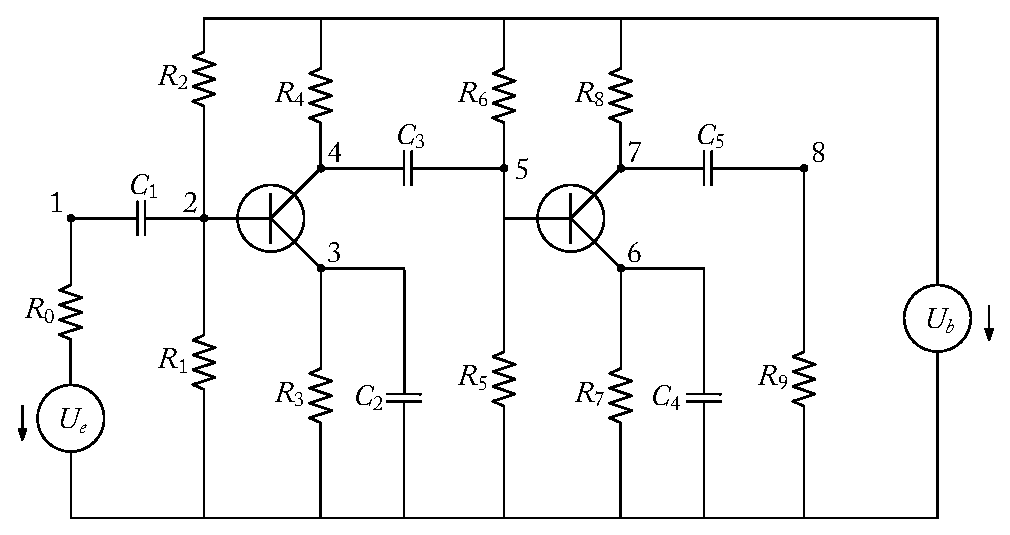
\includegraphics[width=0.7\textwidth]{figures/chapter_4/transistor_amplifier.eps}
  \caption{Eight-node transistor-amplifier circuit~\cite{lioen1998test, mazzia2008test}.}
  \label{chap5:fig:transistor_amplifier}
\end{figure}

The index reduction process is smoothly performed, and the complexity of the expressions encountered throughout the index reduction is detailed in Table~\ref{chap5:tab:tppc_robot}. As we can see, the expression complexity is not affected by the index reduction process. The numerical integration of the reduced \ac{DAE} system is performed using both the \Maple{} and \Indigo{} numerical solvers. In this regard, \Maple{}, \Mathematica{}, \Matlab{} (both Pantelides and Gaussian elimination), and \Indigo{} can integrate the original \ac{DAE} system in the specified time interval $t \in \RSI{0}{0.2}{\second}$.

\begin{figure}[htb]
  \centering
  \small{\includetikz{figures/chapter_4/transistor_amplifier.tex}}
  \caption{Transistor amplifier circuit integration results~\cite{lioen1998test, mazzia2008test} in the time interval $t \in \RSI{0}{0.2}{\second}$. Notice that the output signal $U_8$ is equal to the state variable $x_8$. \emph{Legend}: \textcolor{mycolor1}{$\blacksquare$} input signal $U_e(t)$, and \textcolor{mycolor2}{$\blacksquare$} output signal $U_8$.}
  \label{chap5:fig:transistor_amplifier_results}
\end{figure}

\begin{table}
  \caption{Expression complexity encountered throughout the index reduction of the eight-node transistor-amplifier problem~\cite{lioen1998test, mazzia2008test} \ac{DAE} system. \emph{Legend}: $\cf$ = functions, $\ca$ = additions, $\cm$ = multiplications, and $\cd$ = divisions.}
  \label{chap5:tab:tppc_robot}
  \centering
  {\footnotesize\begin{tabular}{cccc}
    \multicolumn{4}{c}{\textbf{Eight-Nodes Transistor-Amplifier~\cite{lioen1998test, mazzia2008test}}} \\
    \toprule
    \textbf{Original \acp{DAE}} & \multicolumn{3}{c}{$\mF = 55\cf + 21\cd + 29\cm + 41\ca$ \quad $\mh = 0$} \\
    \midrule
    \textbf{Reduction step} & $\mE$ & $\mg$ & $\ma$ \\
    \midrule
    Index-1 \acp{DAE} & $5\ca$ & $17\cf + 11\cd + 22\cm + 20\ca$ & $19\cf + 12\cd + 44\cm + 24\ca$ \\
    Index-0 \acp{DAE} & $24\cf + 26\cd + 24\cm + 24\ca$ & $18\cf + 12\cd + 26\cm + 20\ca$ & $0$ \\
    \midrule
    \textbf{Reduced \acp{DAE}} & \multicolumn{3}{c}{$\mF = 74\cf + 26\cd + 87\cm + 49\ca$ \quad $\mh = 19\cf + 12\cd + 44\cm + 26\ca$} \\
    \bottomrule
    \end{tabular}}
\end{table}

\subsection{Electric Ring Modulator}

The electric ring modulator is an interesting example of a system whose structure depends on the specific values of the parameters. The system is in the form $\m{M}\m{x}^\prime = \m{f}(\m{x},t)$, where $\m{x} = [x_1, \dots, x_{15}]^\top$, $\m{M}$ and $\m{f}(\m{x},t)$ being given by
%
\begin{equation}
  \m{M} = \mathrm{diag}(C, C, C_s, C_s, C_s, C_s, C_p, L_h, L_h, L_{s2}, L_{s3}, L_{s2}, L_{s3}, L_{s1}, L_{s1}) \, \text{,}
\end{equation}
%
\begin{equation}
  \m{f}(\m{x},t) = \begin{bmatrix}
    x_8 - (x_{10} + x_{11})/2 + x_{14} - x_1/R \\
    x_9 - (x_{12} + x_{13})/2 + x_{15} - x_2/R \\
    x_{10} - q(U_{d1}) + q(U_{d4}) \\
    -x_{11} + q(U_{d2}) - q(U_{d3}) \\
    x_{12} + q(U_{d1}) - q(U_{d3}) \\
    -x_{13} - q(U_{d2}) + q(U_{d4}) \\
    -x_7/R_p + q(U_{d1}) + q(U_{d2}) - q(U_{d3}) - q(U_{d4}) \\
    x_1 \\
    x_2 \\
    x_1/2 - x_3 - R_{g2}x_{10} \\
    -x_1/2 + x_4 - R_{g3}x_{11} \\
    x_2/2 - x_5 - R_{g2}x_{12} \\
    -x_2/2 + x_6 - R_{g3}x_{13} \\
    -x_1 + U_{in1}(t) - (R_i + R_{g1})x_{14} \\
    -x_2 - (R_c+R_{g1})x_{15}
  \end{bmatrix} \, \text{,}
\end{equation}
%
where
%
\begin{equation*}
  \begin{array}{l}
    U_{d1} = x_3 - x_5 - x_7 - U_{in2}(t) \, \text{,} \\
    U_{d2} = -x_4 + x_6 - x_7 - U_{in2}(t) \, \text{,} \\
    U_{d3} = x_4 + x_5 + x_7 + U_{in2}(t) \, \text{,} \\
    U_{d4} = -x_3 - x_6 + x_7 + U_{in2}(t) \, \text{,} \\
    q(U) = \gamma(exp(\delta U) - 1) \, \text{,} \\
    U_{in1}(t) = 1/2 \sin(2000 \pi t) \, \text{,} \\
    U_{in2}(t) = 2 \sin(20000 \pi t) \, \text{.}
  \end{array}
\end{equation*}
%
\acp{IC} at $t = 0$ and parameters are given by $\m{x}_0 = [0, 0, 0, 0, 0, 0, 0, 0, 0, 0, 0, 0, 0, 0, 0]^\top$, and
%
\begin{equation*}
  \begin{array}{l}
    C = \SI{16}{\nano\farad} \, \text{,} \\
    C_s = 0~\text{or}~\SI{2}{\pico\farad} \, \text{,} \\
    C_p = \SI{100}{\nano\farad} \, \text{,} \\
    L_h = \SI{4.45}{\henry} \, \text{,} \\
    L_{s1} = \SI{2}{\milli\henry} \, \text{,} \\
    L_{s2} = \SI{0.5}{\milli\henry} \, \text{,} \\
    L_{s3} = \SI{0.5}{\milli\henry} \, \text{,} \\
    \gamma = 40.67286402 \, \text{,} \\
  \end{array}
  \qquad
  \begin{array}{l}
    R = \SI{25}{\kilo\ohm} \, \text{,} \\
    R_p = \SI{50}{\ohm} \, \text{,} \\
    R_{g1} = \SI{36.3}{\ohm} \, \text{,} \\
    R_{g2} = \SI{17.3}{\ohm} \, \text{,} \\
    R_{g3} = \SI{17.3}{\ohm} \, \text{,} \\
    R_{i} = \SI{50}{\ohm} \, \text{,} \\
    R_{c} = \SI{600}{\ohm} \, \text{,} \\
    \delta = 17,7493332 \, \text{.} \\
  \end{array} \, \text{.}
\end{equation*}
%
It must be pointed out that if $C_s \neq 0$, the system is an \acp{ODE}, otherwise, it is an index-2 \ac{DAE} system. In the original test problem in~\cite{lioen1998test, mazzia2008test}, the authors set $C_s = \SI{2}{\pico\farad}$ to obtain an \ac{ODE} system. In Figure~\ref{chap5:fig:ring_modulator}, the electric ring modulator circuit is shown.

Considering $C_s = 0$, the index reduction process is flawlessly performed through the presented algorithm, complexity of the expressions encountered throughout the index reduction is detailed in Table~\ref{chap5:tab:tppc_robot}. Numerical integration in the specified time interval $t \in \RSI{0}{1}{\milli\second}$ is successfully performed by \Indigo{} numerical solvers. Conversely, \Maple{} is not able to integrate the original \ac{DAE} due to computational time exceeding \SI{100}{\second}. Results of the numerical integration are shown in Figure~\ref{chap5:fig:ring_modulator_results}, where the modulated output signal $U_2$ is represented. Notice that the modulated output signal is strongly influenced by the $C_s = 0$ assumption.

\begin{figure}
  \centering
  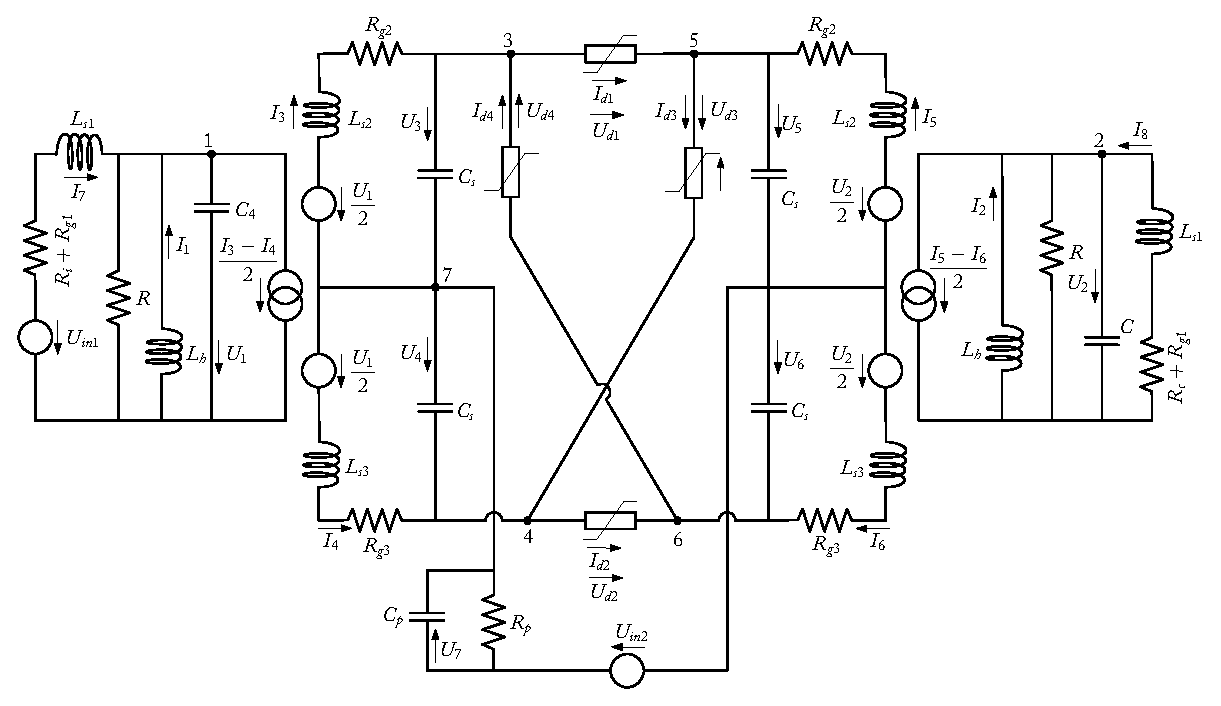
\includegraphics[width=1.0\textwidth]{figures/chapter_4/ring_modulator.eps}
  \caption{Electric ring modulator circuit~\cite{lioen1998test, mazzia2008test}.}
  \label{chap5:fig:ring_modulator}
\end{figure}

\begin{table}
  \caption{Expression complexity encountered throughout the index reduction of the electric ring modulator problem~\cite{lioen1998test, mazzia2008test} \ac{DAE} system. \emph{Legend}: $\cf$ = functions, $\ca$ = additions, $\cm$ = multiplications, and $\cd$ = divisions.}
  \label{chap5:tab:tppc_robot}
  \centering
  {\footnotesize\begin{tabular}{cccc}
    \multicolumn{4}{c}{\textbf{Electric Ring Modulator~\cite{lioen1998test, mazzia2008test}}} \\
    \toprule
    \textbf{Original \acp{DAE}} & \multicolumn{3}{c}{$\mF = 116\cf + 3\cd + 75\cm + 92\ca$ \quad $\mh = 0$} \\
    \midrule
    \textbf{Reduction step} & $\mE$ & $\mg$ & $\ma$ \\
    \midrule
    Index-2 \acp{DAE} & $0$ & $51\cf + 3\cd + 41\cm + 41\ca$ & $44\cf + 32\cm + 36\ca$ \\
    Index-1 \acp{DAE} & $86\cf + 68\cm + 66\ca$ & $262\cf + 13\cd + 416\cm + 220\ca$ & $10\cf + 2\cd + 18\cm + 11\ca$ \\
    Index-0 \acp{DAE} & $86\cf + 12\cd + 72\cm + 70\ca$ & $262\cf + 13\cd + 416\cm + 220\ca$ & $0$ \\
    \midrule
    \textbf{Reduced \acp{DAE}} & \multicolumn{3}{c}{$\mF = 335\cf + 15\cd + 537\cm + 256\ca$ \quad $\mh = 54\cf + 2\cd + 50\cm + 47\ca$} \\
    \bottomrule
    \end{tabular}}
\end{table}

\begin{figure}[htb]
  \centering
  \small{\includetikz{figures/chapter_4/ring_modulator.tex}}
  \caption{Electric ring modulator circuit integration results~\cite{lioen1998test, mazzia2008test} in the time interval $t \in \RSI{0}{1}{\milli\second}$. The lines represent the modulated output signal $U_2$, which is equal to the state variable $x_2$. \emph{Legend}: \textcolor{mycolor1}{$\blacksquare$} output signal $U_2$ with $C_s = \SSI{0}{\pico\farad}$ (\ac{DAE} system), \textcolor{mycolor2}{$\blacksquare$} output signal $U_2$ with $C_s = \SSI{2}{\pico\farad}$ (\ac{ODE} system).}
  \label{chap5:fig:ring_modulator_results}
\end{figure}

\subsection{Cascade of Differential Amplifiers}

The cascade of differential amplifiers is an example of a system whose index can be arbitrarily high, depending on how many operational amplifiers are cascaded. If we consider a circuit with one differential amplifier as shown in Figure~\ref{chap:4:fig:diffamp_single} and, assuming that the operational amplifier is ideal, the circuit equations lead to the relation $x(t) = -C R U(t)^{\prime}$ where $U(t)$ is the generator voltage. Since the solution to the circuit equations involves at least one derivative of the input function, the system must be index-1. By cascading a series of $p \in \mathcal{N}$ differential amplifiers in a circuit as in Figure~\ref{chap:4:fig:diffamp_cascade}, we can see that the resulting \acp{DAE} index is equal to $p$. Specifically, the voltage at the output of the $p$-th differential amplifier is given by $x_p(t) = -C_p R_p x_{p-1}(t)^{\prime}$, where $v(t) = -C_1 R_1 U(t)^{\prime}$. Thence the following system of equations is obtained
%
\begin{equation*}
  \begin{cases}
    x_1(t) = -C_1 R_1 U(t)^{\prime} \\
    x_2(t) = -C_2 R_2 x_1(t)^{\prime} \\
    ~\vdots \\
    x_p(t) = -C_p R_p x_{p-1}(t)^{\prime}
  \end{cases}
  %
  \quad \text{whose analytical solution is} \quad
  %
  x_i(t) = \prod_{j=1}^{i} (-C_j R_j) \dfrac{\de{}^{i}}{\de{}t^{i}}U(t) \, \text{.}
\end{equation*}
%
Consistent \acp{IC} at $t = t_0$ can be easily obtained by evaluating the analytical solution at $t = t_0$, \ie{},
%
\begin{equation*}
  \m{x}_0 = \begin{bmatrix}
    -C_1 R_1 \left.\dfrac{\de{}}{\de{}t}U(t)\right|_{t=t_0} \\
    \vdots \\
    \displaystyle\prod_{j=1}^{p} (-C_j R_j) \left.\dfrac{\de{}^{p}}{\de{}t^{p}}U(t)\right|_{t=t_0}
  \end{bmatrix} \, \text{.}
\end{equation*}

\begin{figure}[htb]
  \centering
  \begin{subfigure}[t]{0.26\textwidth}
    \centering
    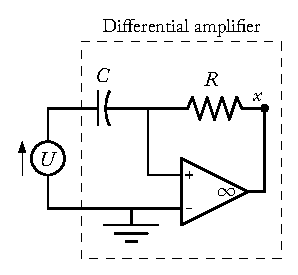
\includegraphics[width=1.0\textwidth]{figures/chapter_4/differential_amplifier_single.eps}
    \caption{Circuit with a single differential amplifier.}
    \label{chap:4:fig:diffamp_single}
  \end{subfigure}%
  \hfill%
  \begin{subfigure}[t]{0.72\textwidth}
    \centering
    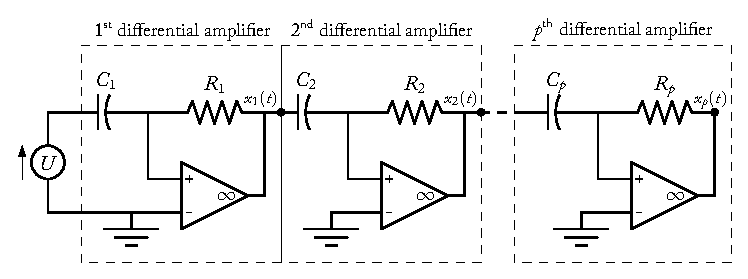
\includegraphics[width=1.0\textwidth]{figures/chapter_4/differential_amplifier_cascade.eps}
    \caption{Circuit with a cascade of $p$ differential amplifiers.}
    \label{chap:4:fig:diffamp_cascade}
  \end{subfigure}
  \caption{Circuit diagrams for the cascade of differential amplifiers problem~\cite{brenan1995numerical}.}
  \label{chap:4:fig:diffamp_all}
\end{figure}

The index reduction of such a system, which falls under the category of linear \acp{DAE}, is pretty much straightforward. \Indigo{} can reduce to index-0 systems made of up to $p = 100$ differential amplifiers, even if the performance of the reduction process is strongly linked to the capabilities of \Maple{} symbolic kernel to deal with sparse large matrices. An interesting aspect that this last application brings to light is how systematically the index reduction process is performed through \Indigo{}. The system is transformed in the form $\mE \, \mxp = \mg$ with $\ma = \m{0}$, which is explicitly given by
%
\begin{equation*}
  \left[\begin{array}{ccc|c}
    -C_2 R_2 & & & 0 \\
    & \ddots & & \vdots \\
    & & -C_p R_p & 0 \\
  \end{array}\right]
  %
  \left[\begin{array}{c}
    x_1^{\prime} \\ \vdots \\ x_{p-1}^{\prime} \\ \hline x_p^{\prime}
  \end{array}\right] = \left[\begin{array}{c}
    x_2 \\ \vdots \\ x_p
  \end{array}\right]
  %
  \quad \text{with} \quad
  %
  \ma = \begin{bmatrix}
    - x_1 - C_1 R_1 \dfrac{\de{}}{\de{}t}U(t)
  \end{bmatrix} \, \text{.}
\end{equation*}
%
Then the index reduction is performed $p$ times, and the system $\mE \, \mxp = \mg$ at the $k$-th index reduction step is equal to
%
\begin{equation*}
  \left[\begin{array}{ccc|c|ccc}
    1 &        &   & \\
      & \ddots &   & \\
      &        & 1 & \\ \hline
      &        &   & & -C_{k+2} R_{k+2} \\
      &        &   & & & \ddots \\
      &        &   & & & & -C_{p} R_{p} \\ \hline
      &        &   & 1 \\
  \end{array}\right]
  %
  \left[\begin{array}{c}
    x_1^{\prime} \\ \vdots \\ x_{k+1}^{\prime} \\ \hline
    x_{k+2}^{\prime} \\ \vdots \\ x_{p-1}^{\prime} \\ \hline
    x_p^{\prime}
  \end{array}\right] = \left[\begin{array}{c}
    -C_1R_1 \dfrac{\de{}^2}{\de{}t^2}U(t) \\
    \vdots \\
    \displaystyle\prod_{j=1}^{k-1} (-C_j R_j) \dfrac{\de{}^k}{\de{}t^k}U(t) \\ \hline
    x_{k+2} \\ \vdots \\ x_p \\ \hline
    \displaystyle\prod_{j=1}^{k} (-C_j R_j) \dfrac{\de{}^{k+1}}{\de{}t^{k+1}}U(t)
  \end{array}\right] \, \text{,}
\end{equation*}
%
with algebraic equations $\ma = \m{0}$ and hidden constraints $\mh = \m{0}$ given by
%
\begin{equation*}
  \ma = \begin{bmatrix}
    -x_{k+1} + \displaystyle\prod_{j=1}^{k+1} (-C_j R_j) \dfrac{\de{}^{k+1}}{\de{}t^{k+1}}U(t)
  \end{bmatrix}
  %
  \quad \text{and} \quad
  %
  \mh = \begin{bmatrix}
    -x_{1} - C_1R_1 \dfrac{\de{}}{\de{}t}U(t) \\
    \vdots \\
    -x_k + \displaystyle\prod_{j=1}^{k} (-C_j R_j) \dfrac{\de{}^{k}}{\de{}t^{k}}U(t)
  \end{bmatrix} \, \text{.}
\end{equation*}
%
Finally, at the $p$\textsuperscript{th} step, the reduced index-0 system is written as
%
\begin{equation*}
  \begin{bmatrix}
    1 & & \\
    & \ddots & \\
    & & 1 \\
  \end{bmatrix}
  %
  \begin{bmatrix}
    x_1^{\prime} \\ \vdots \\ x_p^{\prime}
  \end{bmatrix} = \left[\begin{array}{c}
    -C_1R_1 \dfrac{\de{}^{2}}{\de{}t^{2}}U(t) \\
    \vdots \\
    \displaystyle\prod_{j=1}^{p-1} (-C_j R_j) \dfrac{\de{}^{p}}{\de{}t^{p}}U(t)
  \end{array}\right]
  %
  \quad \text{with} \quad
  %
  \mh = \begin{bmatrix}
    -x_{1} - C_1R_1 \dfrac{\de{}}{\de{}t}U(t) \\
    \vdots \\
    -x_k + \displaystyle\prod_{j=1}^{p} (-C_j R_j) \dfrac{\de{}^{p}}{\de{}t^{p}}U(t)
  \end{bmatrix} \, \text{.}
\end{equation*}
%

% % % % % % % % % % % % % % % % % % % % % % % % % % % % % % % % % % % % % % % %

\section{Summary of Results and Discussion}

It is now time to summarize the results obtained from the experiments and discuss the performance of the presented algorithm. To do so we will consider the following aspects: the symbolic index reduction, the numerical integration, and the overall performance of the algorithm throughout the reduction steps. The results are summarized in Table~\ref{chap5:tab:numerical_integration}, where for each example the solution process is summarized in brief. It is important to highlight that in the same table, the examples are numbered according to the order in which they were presented in this chapter, which will be useful for the discussion that follows.

\subsection{Symbolic Index Reduction}

The first aspect to consider is the symbolic index reduction process. Specifically, the presented algorithm can successfully reduce the index of all the example \ac{DAE} systems here considered. The computational cost of the expressions generated during the index reduction procedure is typically comparable to the original \ac{DAE} system in most of the tests. Additionally, we have seen that the specific type of matrix factorization plays a crucial role in the computational cost of the expressions generated during the index reduction process. In this regard, the ``standard'' \ac{LU} factorization is found to produce better results in terms of computational cost than the \ac{FFLU} factorization. Nonetheless, in examples 3, 6, 7 and 11 the expressions generated during the index reduction procedure are significantly more complex than the original \ac{DAE} system. In these cases, the \Maple{} symbolic computation kernel is not able to perform the simplification within \SI{100}{\second} of \ac{CPU} time and the raw expressions are kept in the following reduction steps. As a consequence, the computational cost inherently increases throughout the following reduction steps. Notably, the \ac{DAE} systems that are hard to simplify are those having a matrix $\mA$ that is strongly dependent on the state variables $\mx$ or equivalently that retains complicated divisions in the vector $\mb$. In these cases, the computational cost of the vector $\ma$ increases significantly due to successive and repeated differentiation and symbolic factorization. In examples 3 and 11, the hierarchical pivoting strategy is thereby used to mitigate the expression swell and ensure the successful index reduction of the \ac{DAE} system. In such examples the veiling strategy proved to be of substantial help, effectively reducing the expression complexities and ensuring the successful index reduction of the \ac{DAE} system. On the other hand, in examples 6 and 7, the hierarchical representation is not used on purpose to understand the impact of the expression swell on the numerical integration process.

For the sake of completeness, also the index reduction algorithms provided by \Matlab{} and \Mathematica{} are tested. The results show that both software tools are able to reduce the index of the \ac{DAE} systems, however, the computational cost of the expressions generated during the index reduction procedure cannot be evaluated due to either the lack of a built-in function to compute the expression complexity or the inability to access the reduced \ac{DAE} systems' expressions.

Another aspect that is important to mention is the sudden increase in computational complexity of the expressions generated in the last reduction steps. Even if such a sudden increase is not critical to the correct index reduction as the presented algorithm is insensitive to expression swell, it does undermine the numerical solution efficiency of the final \ac{DAE} system. This highlights the need for further research on expression swell mitigation techniques in symbolic computation (see Section~\ref{chap3:sec:lem}), as well as the need to use integrators that can handle index-1 \acp{DAE}. Specifically, the detection of linear index-1 variables during the index reduction process is would be beneficial to the minimization of the final \ac{DAE} system complexity. This is particularly important for the numerical integration process, as the more complex the expressions, the more computationally expensive the numerical integration process becomes. Discussion on future work (Section~\ref{chap6:sec:future_work}) will provide insights on new developments in this direction.

\subsection{Numerical Integration}

The numerical integration has also been carried out, with outcomes detailed in Table~\ref{chap5:tab:numerical_integration}. This table reports the performance comparison between the joint index reduction algorithm and numerical integration schemes offered by \Maple{} and those of \Indigo{}. To ensure a fair comparison, both \Maple{} and \Indigo{} utilized the \ac{RKF} 4(5) method for numerical integration of the \ac{DAE} system. Identical error tolerances are applied, with a relative tolerance of $10^{-6}$ and an absolute tolerance of $10^{-7}$. The results illustrate that \Indigo{}'s index reduction algorithm implementation effectively generates numerically stable reduced-index \acp{DAE}, ensuring consistent integration across examples. However, exceptions arise in examples 3, 5, 6, 7, 9, 10, 11, 13, and 14. Specifically, in examples 3, 5, 6, 7, 9, 11, and 13, \Maple{} fails to generate code for the reduced-index system within the expected time frame, thus the integration is not performed. This is due to the complexity of the expressions generated during the index reduction procedure, which overloads the \Maple{}'s \texttt{CodeGeneration} package. On the other hand in examples 10 and 14, the numerical integration can not be performed due to the inability of \Maple{} to verify the consistency of the \ac{IVP}. The \Indigo{} numerical integration is successful in all examples, except for example 11, where it fails to generate the code for the reduced-index system within the expected time frame. This is due to the complexity of the expressions generated during the index reduction procedure, which overloads the \Indigo{}'s \texttt{CodeGeneration} package. Notably, in examples 5, 6 and 7 the integration of the reduced-index system is successfully performed using the non-default implicit RadauIIA5 method. Nonetheless, the high expression swell in these examples leads to a significant increase in the computational cost of the numerical integration, however, the numerical stability is not compromised.

\Mathematica{} and \Matlab{} are also tested for numerical integration. The results show that both software tools are able to integrate the original \ac{DAE} systems in the specified time interval. The only exception is example 11, where both fail to integrate the \ac{DAE} system due to the inability to project the \acp{IC} onto the solution manifold.

It is important to highlight that during the numerical integration, the symbolic code is not regenerated, even if the \ac{DAE} system may locally change its index. Indeed, for some numerical values of states and parameters, the \acp{DAE} system structure may change, leading to numerical instability. While this does pose a potential issue, we have not encountered instability in the integration process. The pivot values were continuously monitored during the numerical integration process to ensure that the \ac{DAE} system structure remains consistent, thereby experimentally proving that the presented pivoting strategy is effective.

\setlength\tabcolsep{2.5pt}
\setlength{\LTcapwidth}{\textwidth}
{\footnotesize\centering\begin{longtable}{lccl}
  \caption{Numerical integration results of the reduced-index \ac{DAE} systems. The table reports the name and reference of the \ac{DAE} system, the index of the system, the integration interval $t \in [t_{\text{ini}}, \, t_{\text{end}}]$, and the outcomes of the whole code generation and integration process for both \Maple{} and \Indigo{}. If not otherwise specified, the tests are integrated using an embedded Runge-Kutta-Fehlberg 4(5) method with a relative tolerance of $10^{-6}$ and an absolute tolerance of $10^{-7}$. The computation time limit is \SI{1000}{\second}, to both generate the necessary code and perform numerical computations. \emph{Legend:} \mycheckmark{} successful code generation and numerical integration, \mycrossmark{} errors in the code generation, numerical integration or time expired, and \mywarnmark{} warnings encountered or non-default settings used in the code generation or numerical integration.}
  \label{chap5:tab:numerical_integration}
  \endfirsthead
  \endhead
  %
  \toprule
  \textbf{Integrated \ac{DAE} system} &
  \multicolumn{3}{l}{\textbf{Integration outcomes and errors}} \\
  \midrule
  \multirow{1}{*}{\textbf{1.~~Particle Motion~\cite{campbell1995constraint}}}
    & \Maple{}       & \mycheckmark{}\phantom{\mywarnmark{}} & Success \\ \cmidrule{2-4}
    \multirow{4}{*}{Index-3 \quad $t \in [0, 400\pi]$ seconds} & \Mathematica{} & \mycheckmark{}\phantom{\mywarnmark{}} & Success \\ \cmidrule{2-4}
    & \multirow{2}{*}{\Matlab{}} & \mycheckmark{}\phantom{\mywarnmark{}} & \texttt{reduceDAEIndex} -- Success \\ \cmidrule{3-4}
    &                            & \mycheckmark{}\phantom{\mywarnmark{}} & \texttt{reduceDAEToODE} -- Success \\ \cmidrule{2-4}\cmidrule{2-4}
    & \Indigo{} & \mycheckmark{}\phantom{\mywarnmark{}} & Success \\ \midrule
  \multirow{1}{*}{\textbf{2.~~Car-Axis~\cite{lioen1998test, mazzia2008test}}}
    & \Maple{}       & \mycheckmark{}\phantom{\mywarnmark{}} & Success \\ \cmidrule{2-4}
    \multirow{4}{*}{Index-3 \quad $t \in [0, 3]$ seconds} & \Mathematica{} & \mycheckmark{}\phantom{\mywarnmark{}} & Success \\ \cmidrule{2-4}
    & \multirow{2}{*}{\Matlab{}} & \mycheckmark{}\phantom{\mywarnmark{}} & \texttt{reduceDAEIndex} -- Success \\ \cmidrule{3-4}
    &                            & \mycheckmark{}\phantom{\mywarnmark{}} & \texttt{reduceDAEToODE} -- Success \\ \cmidrule{2-4}\cmidrule{2-4}
    & \Indigo{} & \mycheckmark{}\phantom{\mywarnmark{}} & Success \\ \midrule
  \multirow{1}{*}{\textbf{3.~~Flexible Slider-Crank~\cite{lioen1998test, mazzia2008test}}}
    & \Maple{}  & \mycrossmark{}\phantom{\mywarnmark{}} & Error, time expired in \texttt{dsolve} \\ \cmidrule{2-4}
    Index-3 \quad $t \in [0, 0.1]$ seconds & \Indigo{} & \mycheckmark{}\phantom{\mywarnmark{}} & Success \\ \midrule
  \multirow{1}{*}{\textbf{4.~~2-Pendula~\cite{pryce1998solving}}}
    & \Maple{}  & \mycheckmark{}\phantom{\mywarnmark{}} & Success \\ \cmidrule{2-4}
    Index-5 \quad $t \in [0, 60]$ seconds & \Indigo{} & \mycheckmark{}\phantom{\mywarnmark{}} & Success \\ \midrule
  \multirow{1}{*}{\textbf{5.~~3-Pendula~\cite{nedialkov2008solvingIII}}}
    & \Maple{}  & \mycrossmark{}\phantom{\mywarnmark{}} & Error, time expired in \texttt{dsolve} \\ \cmidrule{2-4}
    Index-7 \quad $t \in [0, 60]$ seconds & \Indigo{} & \mycheckmark{}\mywarnmark{} & Success with RadauIIA5 method \\ \midrule
  \multirow{1}{*}{\textbf{6.~~4-Pendula~\cite{nedialkov2008solvingIII}}}
    & \Maple{}  & \mycrossmark{}\phantom{\mywarnmark{}} & Error, time expired in \texttt{dsolve} \\ \cmidrule{2-4}
    Index-9 \quad $t \in [0, 60]$ seconds & \Indigo{} & \mycheckmark{}\mywarnmark{} & Success with RadauIIA5 method \\ \midrule
  \multirow{1}{*}{\textbf{7.~~5-Pendula~\cite{nedialkov2008solvingIII}}}
    & \Maple{}  & \mycrossmark{}\phantom{\mywarnmark{}} & Error, time expired in \texttt{dsolve} \\ \cmidrule{2-4}
    Index-11 \quad $t \in [0, 60]$ seconds & \Indigo{} & \mycheckmark{}\mywarnmark{} & Success with RadauIIA5 method \\ \midrule
  \multirow{1}{*}{\textbf{8.~~Double-Wishbone Suspension}}
    & \Maple{}  & \mycheckmark{}\phantom{\mywarnmark{}} & Success \\ \cmidrule{2-4}
    Index-3 \quad $t \in [0, 60]$ seconds & \Indigo{} & \mycheckmark{}\phantom{\mywarnmark{}} & Success \\ \midrule
  \multirow{1}{*}{\textbf{9.~~Initial Stage Space Shuttle Reentry~\cite{brenan1995numerical}}}
    & \Maple{}  & \mycrossmark{}\phantom{\mywarnmark{}} & Error, time expired in \texttt{dsolve} \\ \cmidrule{2-4}
    Index-3 \quad $t \in [332.8, 419.8]$ seconds & \Indigo{} & \mycheckmark{}\phantom{\mywarnmark{}} & Success \\ \midrule
  \multirow{1}{*}{\textbf{10.~~Final Stage Space Shuttle Reentry~\cite{brenan1995numerical}}}
    & \Maple{}  & \mycrossmark{}\phantom{\mywarnmark{}} & Error, in \texttt{dsolve/numeric/DAE/checkconstraints} \\ \cmidrule{2-4}
    Index-2 \quad $t \in [0, 300]$ seconds & \Indigo{} & \mycheckmark{}\phantom{\mywarnmark{}} & Success \\ \midrule
  \multirow{1}{*}{\textbf{11.~~Robotic Arm~\cite{pryce1998solving}}}
    & \Maple{}       & \mycrossmark{}\phantom{\mywarnmark{}} & Error, time expired in \texttt{dsolve} \\ \cmidrule{2-4}
    \multirow{4}{*}{Index-5 \quad $t \in [0, 2]$ seconds}
    & \Mathematica{} & \mycrossmark{}\phantom{\mywarnmark{}} & Error, time expired in \texttt{NDSolve} \\ \cmidrule{2-4}
    & \multirow{2}{*}{\Matlab{}} & \mycrossmark{}\phantom{\mywarnmark{}} & \texttt{reduceDAEIndex} -- Error, index reduction not completed \\ \cmidrule{3-4}
    &                            & \mycrossmark{}\phantom{\mywarnmark{}} & \texttt{reduceDAEToODE} -- Error, in \texttt{sym/decic} \\ \cmidrule{2-4}
    & \Indigo{} & \mycrossmark{}\phantom{\mywarnmark{}} & Error, time expired in \texttt{CodeGeneration} \\ \midrule
  \multirow{1}{*}{\textbf{12.~~8-Nodes Transistor-Amplifier~\cite{lioen1998test, mazzia2008test}}}
    & \Maple{}       & \mycheckmark{}\mywarnmark{} & Warning, function evaluations limit exceeded \\ \cmidrule{2-4}
    \multirow{4}{*}{Index-1 \quad $t \in [0, 0.2]$ seconds} & \Mathematica{} & \mycheckmark{}\phantom{\mywarnmark{}} & Success \\ \cmidrule{2-4}
    & \multirow{2}{*}{\Matlab{}} & \mycheckmark{}\phantom{\mywarnmark{}} & \texttt{reduceDAEIndex} -- Success \\ \cmidrule{3-4}
    &                            & \mycheckmark{}\phantom{\mywarnmark{}} & \texttt{reduceDAEToODE} -- Success \\ \cmidrule{2-4}\cmidrule{2-4}
    & \Indigo{} & \mycheckmark{}\phantom{\mywarnmark{}} & Success \\ \midrule
  \multirow{1}{*}{\textbf{13.~~Electric Ring Modulator~\cite{lioen1998test, mazzia2008test}}}
    & \Maple{}  & \mycrossmark{}\phantom{\mywarnmark{}} & Error, time expired in \texttt{dsolve} \\ \cmidrule{2-4}
    Index-2 \quad $t \in [0, 1]$ milliseconds & \Indigo{} & \mycheckmark{}\phantom{\mywarnmark{}} & Success \\ \midrule
  \multirow{1}{*}{\textbf{14.~~Cascaded Differential Amplifiers~\cite{brenan1995numerical}}}
    & \Maple{}  & \mycrossmark{}\phantom{\mywarnmark{}} & Error, in \texttt{dsolve/numeric/DAE/checkconstraints} \\ \cmidrule{2-4}
    Arbitrary high index \quad $t \in [0, 10]$ seconds & \Indigo{} & \mycheckmark{}\phantom{\mywarnmark{}} & Success \\
  \bottomrule
  %
\end{longtable}}


%!TEX root = ../main.tex

\chapter[DAEs Index Reduction and Numerical Solution]{Differential-Algebraic Equations Index Reduction and Numerical Solution}
\label{chap6:daes}

\subsubsection{Copyright Notice}
Part of this chapter has been first published in
%
\begin{center}
  \begin{minipage}{0.9\textwidth}
    \fullcite{stocco2024symbolic}
  \end{minipage}
\end{center}
\begin{center}
  \begin{minipage}{0.9\textwidth}
    \fullcite{stocco2024matrix}
  \end{minipage}
\end{center}
%
by Springer and Elsevier, respectively. Reproduced with permission from Springer and Elsevier.

\begin{center}
  $\ast$~$\ast$~$\ast$
\end{center}

We present an algorithm for the index reduction of first-order differential-algebraic equations. The proposed approach can be applied to generic differential-algebraic equations and exploits neither a priori knowledge nor ad hoc techniques to leverage the specific formulation of the system. The index reduction is performed only by using symbolic manipulation and linear algebra techniques. It is based on the successive separation of the differential and algebraic equations of the system and the subsequent differentiation of the algebraic part. Improved symbolic matrix factorization is used to perform the differential-algebraic equations partitioning, ensure numerical stability, and limit the expression swell of the reduced-index system. The effectiveness of the algorithm is validated through symbolic-numerical examples on a wide range of systems, including physical systems, engineering applications, and ``artificial'' differential-algebraic equations with specific properties. The proposed symbolic index reduction algorithm is implemented in \Maple{} as part of an open-source library.

% % % % % % % % % % % % % % % % % % % % % % % % % % % % % % % % % % % % % % % %

\section{Introduction}
\label{chap6:sec:introduction}

\acp{DAE} are extensively used in dynamic system modeling. The challenge in numerically solving a \ac{DAE} system is assessed through its differentiation index, commonly referred to as ``the'' index~\cite{campbell1995index}. Achieving accurate simulations necessitates converting high-index \acp{DAE} into low-index counterparts, posing a well-recognized challenge~\cite{petzold1982differential}. This process involves transforming a \ac{DAE} system into an equivalent system with a lower index through successive differentiation of the system equations. For this reason, the differentiation index is roughly defined as the number of times algebraic equations are differentiated to obtain an equivalent system of \acp{ODE} with invariants. Index reduction is a crucial step prior to the numerical integration of \acp{DAE}, as integrating high-index systems can be impractical. The primary obstacle lies in the necessity to solve nonlinear systems of equations at each integration step, which can be computationally expensive and, in certain cases, numerically unstable. Specific numerical techniques, introduced in~\cite{petzold1982differential, thomsen1999numerical, baumgarte1972stabilization}, have been developed to address this challenge. However, these methods are not universally effective and may be inapplicable to some high-index \acp{DAE}. Consequently, index reduction becomes an indispensable preliminary stage before numerical integration~\cite{lamour2013differential}.

Given its complicated nature, index reduction has been the subject of extensive research and is often carried out by leveraging the specific formulation of the \ac{DAE} system, like in the multi-body modeling~\cite{zhou2005implicit, zhou2007symbolic, zhou2007symbolicseq, bayo1988modified, wehage1982generalized}. When the specific formulation of the \ac{DAE} system is not known a priori, or the system is not in a specific form, the index reduction process becomes more challenging. Many current simulation software packages for dynamic systems use index-reduction algorithms based on the \ac{SA} of the system, such as the Pantelides algorithm~\cite{pantelides1988consistent} and the dummy derivatives method~\cite{mattsson1993index}, which are subcases of the Pryce's $\Sigma$-method~\cite{pryce1998solving, pryce2001simple, nedialkov2007solvingI, nedialkov2007solvingII, nedialkov2008solvingIII, nedialkov2015algorithm, tan2016symbolic, mckenzie2017structural}. These algorithms are effective in reducing the index of most of the systems, but they can fail either for numerical cancellations~\cite{iwata2019index} or underestimation of the differentiation index~\cite{pantelides1988consistent, unger1995structural}, like in the case of Rei{\ss}ig's \acp{DAE} family~\cite{reissig2000differential}. Symbolic manipulation is proven to be successful in restating a \acp{DAE} on which the $\Sigma$-method fails to a \acp{DAE} on which the \ac{SA} may succeed~\cite{tan2016symbolic}.

Index reduction based on symbolic-numeric aided \ac{SA} has been successful in handling failures of the Pryce's $\Sigma$-method~\cite{tan2016symbolic} as well as in performing symbolically-informed \ac{SA}~\cite{chowdhry2004symbolic}. This latter \ac{SA} approach, which is named $\sigma v$-method, uses symbolic-numeric \ac{LU} factorization for variable substitution and rank determination on linear constant coefficient \acp{DAE}. A valuable attempt to use pure symbolic manipulation in \acp{DAE} index reduction is presented in~\cite{zhou2005implicit, zhou2007symbolic, zhou2007symbolicseq}, where implicit involutive form and \ac{LU} decomposition are successfully used to reduce the index of a simple constrained multi-body system. It is clear that index reduction algorithms based on pure symbolic matrix factorization represent a viable alternative to classic \ac{SA} techniques. However, symbolic matrix factorization feasibility is strongly tied to the performance of the symbolic computation kernel and its capabilities~\cite{zhou2008fraction}. Large expressions can lead to strong performance degradation of the kernel. Techniques aimed at limiting this decrease of performance while performing symbolic linear algebra operations are presented in~\cite{zhou2006hierarchical, zhou2007symbolic, zhou2007symbolicseq}. In these works, the hierarchical representation of expressions is applied to matrix factorization tasks. Nonetheless, the \LULEM{} package~\cite{carette2006linear}, which implements large expression management strategies in \ac{LU} decomposition, significantly outperforms the \Maple{}'s built-in matrix factorization routines.

Following this brief introduction of the most widely recognized index reduction algorithms, we provide an overview of the specific index reduction algorithms found in current state-of-the-art software. The following list is limited to the most prominent solutions dedicated to dynamic system modeling and simulation that are widely adopted in both academia and industry.
%
\begin{itemize}
  \setlength{\itemsep}{-0.2em}
  \item \Matlab{} uses the Pantelides algorithm~\cite{pantelides1988consistent} to reduce the \acp{DAE} to index-1. Alternatively, or if the latter fails, the more reliable but slower Gaussian elimination algorithm can be employed to obtain an index-0 \ac{DAE} system~\cite{matlab}.
  \item \textsc{Modelica}-based software~\cite{mattsson1997modelica, mattsson1998physical} and \textsc{ModelingToolkit}~\cite{modelingtoolkit} employ the Pantelides algorithm~\cite{pantelides1988consistent} along with the dummy derivatives method~\cite{mattsson1993index} to automatically perform the reduction to index-1 \acp{DAE}.
  \item \Mathematica{} offers a comprehensive suite of index reduction algorithms~\cite{mathematica}. It can reduce the index of \acp{DAE} using the Pantelides~\cite{pantelides1988consistent} or structural matrix~ \cite{unger1995structural, chowdhry2004symbolic} methods. Additionally, it implements dummy derivatives~\cite{mattsson1993index} and projection methods for taking hidden constraints into account during numerical integration.
  \item \Maple{} performs symbolic index reduction within the \texttt{dsolve} function~\cite{maple}. However, the implemented algorithms are not documented or referenced. They are likely to be based on the projection method outlined in~\cite{shmoylova2013simplification}. Notably, the patents by the same authors~\cite{postma2012exact, shmoylova2012method, postma2015exact} discuss techniques for eliminating isolated parameters, extracting parameter sub-expressions from \acp{DAE}, and establishing minimal disconnected clusters of parameter sub-expressions. We would like to point out that this information is to be taken with caution, as \Maple{} does not provide specific references on this topic.
\end{itemize}
%
All the showcased software solutions offer integrators for index-0 and index-1 \acp{DAE}. Depending on the system's stiffness, users can select the most appropriate algorithm for numerically integrating the reduced-index system.

The absence of user-invocable standalone functions within the \Maple{} environment that allows for the automatic index reduction of \acp{DAE}, and the inability to extract both the reduced-index system and invariants from the \texttt{dsolve} function, are the primary motivations of this research. Furthermore, recent advances in symbolic matrix factorization, combined with expressions hierarchical representation techniques, provide valuable tools that enable us to further investigate the applicability of a novel algorithm for the index reduction of \ac{DAE} systems, firstly presented in~\cite{stocco2024symbolic} as a preliminary work. The proposed methodology is similar to the previous work of~\citet{chowdhry2004symbolic} and extends it to generic first-order \acp{DAE}, linear in the states' derivatives. Nonetheless, the proposed algorithm does not work on the structural matrix of the system but on the \ac{DAE} system symbolic expressions. Specifically, the idea of using matrix factorization for variable substitution and rank determination is adopted to iteratively separate the differential and algebraic equations of the system. The algebraic equations are then differentiated to obtain an equivalent system with a lower differentiation index. Not less important, new libraries for symbolic matrix factorization (\LAST{}), large expression management (\LEM{}), and signature computation (\SIG{}) are presented. These libraries are based on the \LULEM{} package and extend the work of~\citet{zhou2006hierarchical, carette2006linear} and~\citet{zhou2007symbolic}. The newly presented libraries are designed to ensure the numerical stability of the numerically evaluated expressions, limit the expression swell, and provide an updated object-oriented interface. The effectiveness of the presented index reduction algorithm is validated through symbolic-numerical examples on a wide range of systems, including physical systems, engineering applications, as well as ``artificial'' systems with specific properties. The proposed algorithm is implemented in the \Maple{} environment and is available as a collection of open-source packages~\cite{last2023source,lem2023source}. Furthermore, the insights and the techniques presented in~\cite{zhou2006hierarchical, carette2006linear, zhou2007symbolic} are used to improve the presented algorithm to embed the hierarchical representation of expressions in a future implementation of the algorithm.

The manuscript is organized as follows. After this introduction (Section~\ref{chap6:sec:introduction}), the index reduction algorithm is presented in Section~\ref{chap6:sec:algorithm}. The expression swell mitigation, as well as the details on the symbolic matrix factorization, are discussed in Sections~\ref{chap6:sec:expression_swell} and \ref{chap6:sec:matrix_factorization}. The effectiveness of the algorithm is showcased through symbolic-numerical examples in Section~\ref{chap6:sec:examples}. Finally, Sections~\ref{chap6:sec:future_work} and~\ref{chap6:sec:conclusions} report future developments and conclusions respectively. In~\ref{chap6:sec:cokernel} details on cokernel computation are reported. The newly developed object-oriented symbolic linear algebra (\ref{chap6:sec:last}), large expression management (\ref{chap6:sec:lem}) and signature computation (\ref{chap6:sec:signature}) package descriptions are also included in the appendices. The symbolic index reduction algorithm is implemented in the \Maple{} language and is available as part of the open-source \Indigo{} library~\cite{indigo2023source}. Its usage is illustrated in~\ref{chap6:sec:index_reduction}. Notice that throughout the manuscript the \texttt{teletype} font indicates the use of \Maple{} and \Matlab{} commands or software implementations.

% % % % % % % % % % % % % % % % % % % % % % % % % % % % % % % % % % % % % % % %

\section{Index Reduction Algorithm}
\label{chap6:sec:algorithm}

In this section, we explore the theoretical aspect of reducing the differential index of \ac{DAE} systems. Specifically, to systematically reduce the \ac{DAE} system's index, a novel iterative algorithm is presented. This algorithm comprises two main phases: initially, the separation of the differential equations from the algebraic equations inherent in \acp{DAE}; and subsequently, the differentiation of the algebraic ones to obtain an equivalent system with a reduced index. The algorithm that is presented in this section is implemented in the \Maple{} environment and is available as an open-source package~\cite{indigo2023source}.

\subsection{Differential and Algebraic Equations Separation}
\label{chap6:sec:separation}

The initial phase of the index reduction procedure involves the partitioning of the \ac{DAE} system into its differential and algebraic equations. While in the case of small systems this can be accomplished through manual identification and isolation of the algebraic equations, this approach is inconvenient when dealing with large systems. An alternative method for automating the separation process leverages the cokernel, or left null space, of the \ac{DAE} system matrix, which is computed through matrix factorization techniques. The usage of the cokernel offers a more efficient and reliable means of accomplishing the separation task, variable substitution and not less importantly rank determination.

Consider a first-order system of \acp{DAE} $\mF$ of the form
%
\begin{equation}
  \label{chap6:eq:daes}
  \mF \overset{\mathrm{def}}{=}\mA \, \mxp - \mb = \m{0}.
\end{equation}
%
We denote the cokernel and its orthogonal complement of $\mA$ with $\mK$ and $\mN$ respectively (see~\ref{chap6:sec:cokernel} for details on the cokernel computation with symbolic matrix factorization). Notice that the cokernel is the subspace obtained by the span of $\mK$'s columns. For this reason, hereafter, we refer to the cokernel as the matrix $\mK$ whose columns span the cokernel. Using $\mK$ and $\mN$ it is possible to separate the algebraic part of the \acp{DAE}~\eqref{chap6:eq:daes} as
%
\begin{equation}
  \label{chap6:eq:separated_daes}
  \begin{cases}
    \mE \, \mxp = \mg \\[0.1em]
    \ma = \m{0}
  \end{cases} \text{,} \quad \text{where} \qquad \mA = \begin{bmatrix}
    \mE \\[0.2em]
    \m{0}
  \end{bmatrix} \text{,}
  \quad \text{and} \quad
  \mb = \begin{bmatrix} \mg \\[0.2em] \ma \end{bmatrix} \text{.}
\end{equation}
%
The separated equations of the \acp{DAE} are obtained by the left product of $\mK$ and $\mN$ as
%
\begin{equation}
  \begin{array}{l@{~}c@{~}l}
    \mE &=& \mN \, \mA \text{,} \\[0.1em]
    \mg &=& \mN \, \mb \text{,} \\[0.1em]
    \ma &=& \mK \, \mb \text{.}
  \end{array}
\end{equation}
%
This results in an equivalent \ac{DAE} system, where the algebraic equations $\ma$ are now explicit. The details of the cokernel and its orthogonal complement computation are discussed in~\ref{chap6:sec:cokernel}.

\subsection{Algebraic Equations Differentiation}
\label{chap6:sec:differentiation}

The algebraic equations in the \ac{DAE} system~\eqref{chap6:eq:separated_daes} are now differentiated as
%
\begin{equation}
  \label{chap6:eq:diff_daes}
  \dfrac{\mathrm{d}}{\mathrm{d}t} \ma = \mAd \, \mxp - \mgd \text{.}
\end{equation}
%
The \acp{DAE}~\eqref{chap6:eq:separated_daes} after differentiation of algebraic equations now take a form similar to that of~\eqref{chap6:eq:daes}, where
%
\begin{equation}
  \label{chap6:eq:reduced_daes}
  \mA = \begin{bmatrix} \mE \\[0.2em] \mAd\end{bmatrix} \text{,}
  \quad \text{and} \quad
  \mb = \begin{bmatrix} \mg \\[0.2em] \mgd\end{bmatrix} \text{.}
\end{equation}
%
The set of invariants, which are collected in $\mh$, is updated adding the algebraic equations $\ma$
%
\begin{equation}
  \mh \quad \xleftarrow[\text{update}]{\text{\, Invariants \,}} \quad \overset{{\text{The old $\mh$}}}{\begin{bmatrix} \overbrace{\mh} \\[0.2em] \ma \end{bmatrix}}.
\end{equation}
%
The iterative procedure, involving the sequential separation and differentiation of the algebraic segment of the system, is iterated until $\mA$ is non-singular. When $\mA$ is non-singular the \ac{DAE} corresponds to a system of \acp{ODE} compounded by the invariants $\mh$, which are the collection of the hidden constraints produced in the index reduction process. The invariants $\mh$ can be initialized empty or with user-defined algebraic equations aimed at preserving crucial system properties, such as energy conservation and/or momentum conservation. A pseudocode and a flowchart of the index reduction algorithm can be found in Algorithm~\ref{chap6:alg:index_reduction} and \figurename~\ref{chap6:fig:index_reduction}, respectively.

\begin{figure}[htp!]
  \centering
  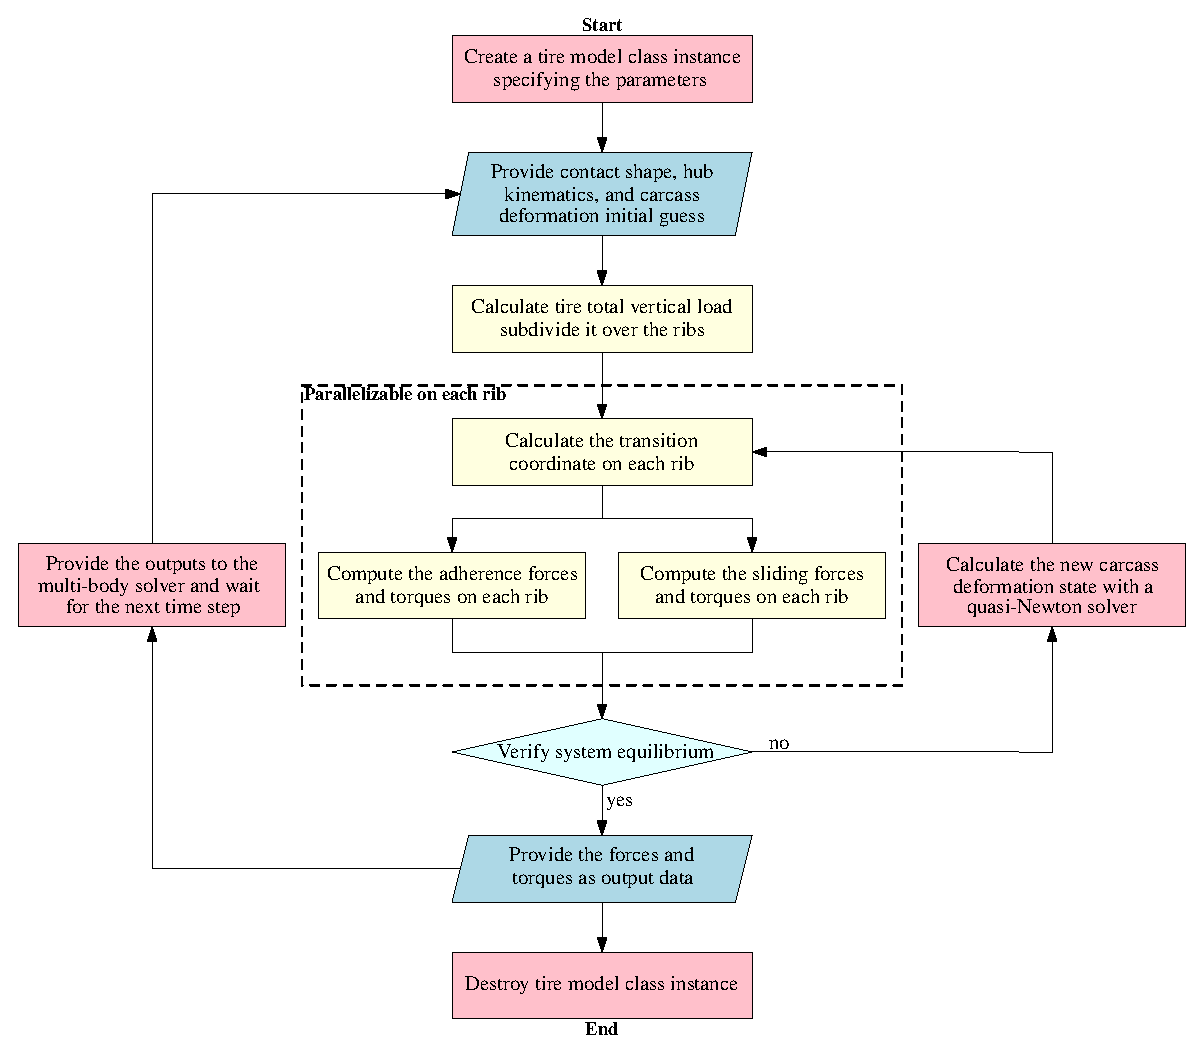
\includegraphics[angle=90, width=0.9\columnwidth]{flowchart}
  \caption{Flowchart of the index reduction algorithm.}
  \label{chap6:fig:index_reduction}
\end{figure}

\begin{algorithm}[H]
  \caption{Index reduction algorithm.}
  \label{chap6:alg:index_reduction}
  \begin{algorithmic}[1]
    \State \textbf{Require:} A \ac{DAE} system of the form $\mF \overset{\mathrm{def}}{=} \mA \, \mxp - \mb = \m{0}$.
    \Procedure{ReduceIndex}{$\mF$} \Comment{Index reduction procedure}
      \State $\mh \gets \varnothing$ \Comment{The set of invariants}
      \State $\mA, \, \mb \gets \mathrm{GenerateMatrix}(\mF, \, \mxp)$ \Comment{The \ac{DAE} system matrix}
      \State $m \gets \mathrm{Size}(\mx)$\Comment{The size of $\mx$}
      \While{$\mA$ is singular}
        \State $\displaystyle\triangleright$ Differential and algebraic equations separation (Section~\ref{chap6:sec:separation})
        \State $\mL, \, \mU, \, \mP, \, \mQ \gets \mathrm{MatrixFactorization}(\mA)$ \Comment{LU or FFLU decomposition of $\mA$}
        \State $r \gets \mathrm{Rank}(\mU)$ \Comment{The rank of $\mU$ is equal to the rank of $\mA$}
        \State $\mI_1 \gets \mathrm{IdentityMatrix}(r, \, r)$ \Comment{The upper identity matrix}
        \State $\mI_2 \gets \mathrm{IdentityMatrix}(m-r, \, m-r)$ \Comment{The lower identity matrix}
        \State $\mE \gets [\mI_1, \, \m{0}] \, \mU \, \mQ^\top$ \Comment{The reordered part of $\mA$}
        \State $\mg \gets [\mI_1, \, \m{0}] \, \mL^{-1} \, \mP \, \mb$ \Comment{The differential part of $\mb$}
        \State $\ma \gets [\m{0}, \, \mI_2] \, \mL^{-1} \, \mP \, \mb$ \Comment{The algebraic part of $\mb$}
        \State
        \State $\displaystyle\triangleright$ Algebraic equations differentiation (Section~\ref{chap6:sec:differentiation})
        \State $\mAd, \, \mgd \gets \mathrm{GenerateMatrix}(\mathrm{Diff}(\ma, \, t), \, \mxp)$ \Comment{Differentiate the equations $\ma$}
        \State $\mA \gets \begin{bmatrix} \mE \\ \mAd \end{bmatrix}$ \quad and \quad $\mb \gets \begin{bmatrix}\mg \\ \mgd \end{bmatrix}$
        \Comment{The new matrix $\mA$ and vector $\mb$}
        \State $\mh \gets \mh \cup \ma$ \Comment{Add the algebraic equations to the set of invariants}
      \EndWhile \\
      \Return $\mA, \, \mb, \, \mh$ \Comment{The \acp{DAE} reduced to an \ac{ODE} system with invariants}
    \EndProcedure
  \end{algorithmic}
\end{algorithm}

\subsection{A Step-by-Step Example}
\label{chap6:sec:step_by_step}

Within this Section, we present the step-by-step results of the index reduction algorithm. To do so we exploit a simple non-stiff index-3 problem found in \Wolfram{}~\Mathematica{} documentation~\cite{mathematica}. The initial value problem is defined as follows
%
\begin{equation}
  \label{chap6:eq:index_3}
  \mF = \begin{bmatrix}
    x^{\prime}_{2} - x_{1} - \cos(t) \\
    x^{\prime}_{3} - x_{2} - \sin(t) \\
    x_{3} - \cos(t)
  \end{bmatrix},
\end{equation}
%
with states $\mx = [x_{1}, \, x_{2}, \, x_{3}]^\top$ and initial conditions $\mx_{0} = [-1, \, 0, \, 1]^\top$. Notice that the analytical solution of this problem is $\mx_{exact} = [\sin(t) - 2\cos(t), \, 2\sin(t), \, \cos(t)]^\top$. The index reduction algorithm is applied to the \ac{DAE} system~\eqref{chap6:eq:index_3} and the step-by-step results for the matrices $\mE$, $\mg$, and $\ma$ are reported here below.
%
\begin{equation*}
  \begin{array}{l}
    \text{Index-3 \acp{DAE}:} \quad \mE = \begin{bmatrix} \,
      0 & 1 & 0 \\
      0 & 0 & 1
    \, \end{bmatrix}, \quad
    \mg = \begin{bmatrix} \,
      \sin(t) - x_{1} \\
      \sin(t) - x_{2}
    \, \end{bmatrix}, \quad\quad~~~\,
    \ma = \begin{bmatrix} \,
      \cos(t) - x_{3}
    \, \end{bmatrix}. \\[1.0em]
    %
    \text{Index-2 \acp{DAE}:} \quad \mE = \begin{bmatrix} \,
      0 & 1 & 0 \\
      0 & 0 & 1
    \, \end{bmatrix}, \quad
    \mg = \begin{bmatrix} \,
      \sin(t) - x_{1} \\
      \sin(t) - x_{2}
    \, \end{bmatrix}, \quad\quad~~~\,
    \ma = \begin{bmatrix} \,
      2\sin(t) - x_{2}
    \, \end{bmatrix}. \\[1.0em]
    %
    \text{Index-1 \acp{DAE}:} \quad \mE = \begin{bmatrix} \,
      0 & 0 & 1 \\
      0 & 1 & 0
    \, \end{bmatrix}, \quad
    \mg = \begin{bmatrix} \,
      \sin(t) - x_{2} \\
      \sin(t) - x_{1}
    \, \end{bmatrix}, \quad\quad~~~\,
    \ma = \begin{bmatrix} \,
      \sin(t) - 2\cos(t) - x_{1}
    \, \end{bmatrix}. \\[1.0em]
    %
    \text{Index-0 \acp{DAE}:} \quad \mE = \begin{bmatrix} \,
      0 & 0 & 1 \\
      0 & 1 & 0 \\
      1 & 0 & 0
    \, \end{bmatrix}, \quad
    \mg = \begin{bmatrix} \,
      \sin(t) - x_{2} \\
      \sin(t) - x_{1} \\
      2\sin(t) + \cos(t)
    \, \end{bmatrix}, \quad
    \ma = \varnothing.
  \end{array}
\end{equation*}
%
The final form of the system is an index-0 \acp{DAE} system is then
%
\begin{equation}
  \label{chap6:eq:index_3_reduced}
  \mF = \begin{bmatrix}
    x^{\prime}_{2} - x_{1} - \cos(t) \\
    x^{\prime}_{3} - x_{2} - \sin(t) \\
    x^{\prime}_{1} - \cos(t) - 2\sin(t)
  \end{bmatrix},
  %
  \quad \text{with invariants} \quad
  %
  \mh = \begin{bmatrix}
    \cos(t) - x_{3} \\
    2\sin(t) - x_{2} \\
    \sin(t) - 2\cos(t) - x_{1}
  \end{bmatrix}.
\end{equation}
%
%Although the just presented example is not so complex and relevant for a real validation of the algorithm, it is useful to demonstrate the step-by-step results of the index reduction algorithm. Furthermore, the expression complexities encountered throughout the index reduction algorithm applied to the Index-3 problem are reported below in \tablename{}~\ref{chap6:tab:complexity}.

\subsection{Known Issues}

While the algorithm just presented is relatively straightforward to implement, it does have two major sources of potential issues that are both determined by the technology used and the fundamental theory.
%
\begin{itemize}
    \item \emph{Expression complexity}. Symbolic manipulation often leads to a growth in expression complexity. For this reason, expression simplification may not always be feasible due to software limitations or excessive CPU time demands. Making the algorithm insensitive to expression swell is thus crucial to its effectiveness.
    \item \emph{Numerical stability of symbolic matrix factorization}. The description of the algorithm involves the manipulation of matrices and vectors with either symbolic or mixed symbolic-numeric entries. Ensuring that symbolic matrix factorization maintains numerical stability is a critical requirement of the algorithm. In the case of \ac{LU} decomposition, inadequate pivoting strategies can lead to the generation of singular matrices, which in turn can cause the algorithm to fail~\cite{zhou2005implicit, zhou2007symbolic, giesbrecht2014symbolic}.
\end{itemize}
%
These are the two main points that we acknowledge in the implementation of the algorithm. In the forthcoming sections, each of these matters is discussed in detail, with recommendations on techniques and open-source software solutions that are used to address them.

% % % % % % % % % % % % % % % % % % % % % % % % % % % % % % % % % % % % % % % %

\section{Expression Swell}
\label{chap6:sec:expression_swell}

Symbolic computation software, such as \Maple{}, is capable of handling relatively large symbolic expressions. However, the increase in complexity can significantly slow down the execution of the index reduction algorithm discussed earlier, resulting in unacceptably long CPU times. This phenomenon, known as expression swell, is a primary contributor to the degradation of performance in symbolic computation kernels. Expression swell can be categorized into two types: \emph{inherent} and \emph{intermediate}. The latter occurs when a calculation temporarily generates extensive expressions during intermediate steps, en route to a potentially more compact final result. To mitigate this issue, hierarchical representation techniques offer a solution~\cite{zhou2006hierarchical}. The core concept of this hierarchical representation is to conceal (or \emph{veil}) intricate expressions from the user by employing auxiliary variables referred to as \emph{veil variables} (or \emph{veils}) and reveal (or \emph{unveil}) them only when they become strictly necessary. As an expert reader may have noticed, expression swell is directly linked to expression complexity. Specifically, choosing the right balance between the maximum expression complexity and the number of veiling variables is crucial to prevent expression swell and concurrently avoid excessive veiling. To effectively gauge expression complexity, a metric is necessary, and various definitions are available. While previous works have relied on the \Maple{}'s \texttt{length} function, we adopt a different measure: the computational cost, which is determined through the \texttt{cost} function in the \texttt{codegen} package. This approach, as illustrated in the forthcoming examples, offers insensitivity to the number of characters used to represent the expression internally to the symbolic computation kernel, thus ensuring superior control over the final expression size.

\paragraph{Large Expression Management} Specific modules designed to perform large expression management tasks and help the user handle hierarchical representations have been developed and documented in prior research~\cite{carette2006linear, zhou2007symbolic}. Among these, the \Maple{} module \texttt{LargeExpressions} already fulfills this role effectively. However, we have observed some minor limitations within this module, primarily arising from its user interface choices rather than the core concept or the programming technique employed. Consequently, they have refined it into a new, object-oriented package known as \LEM{}~\cite{lem2023source}. This updated version remains adherent to the original but offers enhanced control and straightforward utilization of veil variables. Notably, the object-oriented aspect allows for the creation of multiple instances of \LEM{} objects, thereby ensuring a sharp separation between veil variables to prevent potential conflicts resulting from improper usage. Examples of expression complexity calculation and large expression management are reported in~\ref{chap6:sec:complexity} and~\ref{chap6:sec:lem} respectively.

% % % % % % % % % % % % % % % % % % % % % % % % % % % % % % % % % % % % % % % %

\section{Matrix Factorization}
\label{chap6:sec:matrix_factorization}

As previously mentioned, matrix factorization is a widely employed technique for addressing linear systems. There are several types of decompositions, each with distinct properties and characteristics. The \ac{LU} decomposition ranks among the most commonly used approaches. In the context of purely numerical matrices, the practice aligns well with the theoretical foundations of the algorithm. However, when dealing with matrices consisting of either symbolic or mixed symbolic-numeric entries, the situation becomes more intricate~\cite{zhou2007symbolic}. In exact symbolic linear algebra scenarios, the cost of each operation during factorization can vary due to uncontrolled expression swell~\cite{zhou2006hierarchical}. Furthermore, the presence of symbolic values hinders the guarantee of numerical stability. Consequently, a key objective is to derive an output format that retains the symbolic structure of the input matrix and ensures numerical stability.

\paragraph{Fill-In} After the \ac{LU} factorization of a sparse matrix $\m{A}$, it is common to observe that the joint non-zeroes pattern of $\m{L}$ and $\m{U}$ exhibit either equal or lower sparsity compared to the original non-zero pattern of $\m{A}$. This phenomenon, known as fill-in, increases the number of algebraic operations required for solving linear systems, thereby diminishing performance. To mitigate this issue, specific reordering algorithms can be applied to minimize the fill-in of the factorized matrix. These algorithms mainly include \emph{nested dissection}~\cite{george1973nested, lipton1979generalized} and \emph{minimum degree}~\cite{markowitz1957elimination, rose1970symmetric} techniques. In this work, the minimum degree algorithm is preferred due to its ease of implementation. Conversely, the nested dissection is not yet considered as it involves working on the system's graph to identify graph separators, which is a less straightforward process in the symbolic case.

\paragraph{Numerical Stability} A crucial concern is ensuring the numerical stability of the symbolic code generated by matrix factorization. This issue is closely tied to \emph{zero-} or \emph{identity-testing} within symbolic expressions. When simplifying an expression is not feasible, the most commonly adopted methods for zero-testing are the probabilistic ones, which rely on the \emph{DeMillo-Lipton-Schwarz-Zippel lemma}~\cite{demillo1978probabilistic, schwartz1980fast, zippel1979probabilistic}.
%
\begin{itemize}
    \item The utilization of \emph{signature functions} involves the verification of equivalent expressions within a multitude of sub-expressions, a process facilitated by \emph{hashing} techniques~\cite{gonnet1984determining, char1984design, gonnet1986results, monagan1994signature}. In \Maple{}, each expression is stored in the simplification table, employing its signature as a key. A unique feature of these signatures is that equivalent expressions share the same signature. It is important to note that not all expressions can have their signatures determined, such as trigonometric expressions, however, opportune coordinates change for signature computation routines can be applied (see~\ref{chap6:sec:signature}).
    %
    \item The \emph{Hybrid symbolic-numerical} or \emph{static pivoting approach} offers a means to validate the stability of symbolic code through random numerical evaluations~\cite{giesbrecht2014symbolic, li1998making}. While this approach may be computationally less efficient compared to the former method, it yields satisfactory results. In other words, the ``choice of pivots is numerically good at most numerical specializations'' as emphasized in~\cite{giesbrecht2014symbolic}.
\end{itemize}

Based on these observations, the \ac{LU} and \ac{FFLU} factorizations are preferred over the QR and \ac{GJ} factorizations, as the former two involve simpler operations, thereby mitigating the issue of expression swell. Additionally, employing the \ac{LU} factorization with a minimum degree pivoting strategy proves superior in reducing fill-in.

\subsection{Improved Symbolic Pivoting Strategy}

A crucial detail of any \ac{LU}-based decomposition, either numerical or symbolic, is the pivoting strategy. This strategy hinges on the two aforementioned considerations: the degrees of the elements within the system matrix and the actual complexity of the expressions. The elements in the system matrix are arranged in descending order of their degrees, and the pivot of the least complexity is chosen. Sometimes these two features are conflicting. In such cases, the prioritization of the pivot with the lowest degree is preferred. It is important to notice that pivots consisting of numerical values take precedence over those with symbolic values, primarily due to their inherent minimum expression complexity. Throughout the pivoting process, the utilization of signatures is also employed whenever possible to confirm the presence of null expressions without the need for simplification. To summarize, the main steps of the pivoting strategy are the following.
%
\begin{enumerate}
  \item The degree for each of the system matrix's entries is calculated.
  \item The pivots are sorted by degree and a permutation is generated.
  \item The pivots are iterated in the order of the permutation and a candidate pivot is selected at each step.
  \item The candidate pivot is checked for null expressions with the aid of signatures.
  \item If the candidate pivot signature is not null, the expression is simplified and their complexity is calculated.
  \item If the candidate pivot is numeric, its numerical value is calculated, otherwise, it is set to infinity.
  \item The candidate pivot with the lowest complexity or largest absolute numeric value is selected as the best pivot and returned.
\end{enumerate}
%
A detailed description of the developed symbolic pivoting strategy is presented in Algorithm~\ref{chap6:alg:pivoting_strategy}.

\begin{algorithm}[H]
  \caption{Symbolic Pivoting Strategy.}
  \label{chap6:alg:pivoting_strategy}
  \begin{algorithmic}[1]
    \State \textbf{Require:} A $n \times m$ matrix $\m{A}$.
    \State \phantom{\textbf{Require:}} The $k$-th pivoting stage.
    \Procedure{SymbolicPivoting}{$\m{A}$, $k$} \Comment{Symbolic pivoting procedure for the $k$-th pivot}
    \State $\m{d}^r, \, \m{d}^c \gets \text{ComputeDegrees}(\m{A})$ \Comment{Calculate the row and column degrees of $\m{A}$}
    \For{$i$ \textbf{from} $k$ \textbf{to} $n$} \Comment{Iterate over the rows}
      \For{$j$ \textbf{from} $k$ \textbf{to} $m$} \Comment{Iterate over the columns}
        \State $D_{ij} \gets \infty$ \Comment{Set the combined degree matrix to infinity}
        \IfThen{$A_{ij} \neq 0$}
        {$D_{ij} \gets d^r_{i} \, \max(0, \, d^c_j-1) + d^c_j \, \max(0, \, d^r_i-1)$} \Comment{Compute the combined degree}
      \EndFor
    \EndFor
    \State $\mathcal{P} \gets \text{Sort}(\m{D})$ \Comment{Find the permutation that sorts the pivots list by degree cost}
    \State $q, \, l \gets \, 0, \, 0$ \Comment{Initialize the temporary pivot row and column indices}
    \State $p, \, p_c, \, p_n \gets \infty, \, \infty, \, \infty$ \Comment{Initialize the temporary pivot value, complexity and numerical value}
    \For{\textbf{all} $(i, j)$ \textbf{in} $\mathcal{P}$} \Comment{Iterate on the permutation set}
      \IfThen{$p_c \neq \infty$ \textbf{and} $D_{ij} > D_{ql}$}{\textbf{break}} \Comment{No more good pivots to check}
      \State $t \gets A_{ij}$ \Comment{Get the pivot value}
      \IfThen{$\text{Signature}(t) = 0$}{\textbf{continue}} \Comment{Skip the next pivot}
      \State $t \gets \text{Simplify}(t)$ \Comment{Try to simplify the pivot expression}
      \State $t_c \gets \text{ExpressionComplexity}(t)$ \Comment{Calculate the computational complexity of the pivot}
      \State $t_n \gets \infty$ \Comment{Set the default numerical value of the pivot to infinity}
      \IfThen{$t$ is numeric}{$t_n \gets \max(1, \, \mathrm{abs}(t))$} \Comment{Set the numerical value of the pivot}
      \If{$t_c < p_c$ \textbf{or} ($t_c = p_c$ \textbf{and} $t_n > p_n$)} \Comment{If the pivot is better than the current one}
        \State $q, \, l \gets i, \, j$ \Comment{Update the best pivot row and column indices}
        \State $p, \, p_c, \, p_n \gets t, \, t_c, \, t_n$ \Comment{Update the best pivot value, complexity and numerical value}
      \EndIf
    \EndFor \\
    \Return $p, \, q, \, l$ \Comment{The $k$-th pivot and its position}
    \EndProcedure
  \end{algorithmic}
\end{algorithm}

\paragraph{Symbolic Linear Algebra} The considerations outlined above aid as the foundations for the \LAST{} package~\cite{last2023source}. Within this package, the pivoting process has been designed to address the critical considerations of expression swell and numerical stability as previously discussed. This toolkit, integrated into the \Maple{} environment, is dedicated to symbolic linear algebra tasks. It builds upon the original research outlined in~\cite{zhou2008fraction} and encompasses a collection of functionalities for symbolic full-pivoting \ac{LU}, \ac{FFLU}, QR, and \ac{GJ} factorizations. Importantly, the \LAST{} package is intended to be used in tandem with the previously presented \LEM{} package~\cite{lem2023source}, contributing to the mitigation of expression swell.

% % % % % % % % % % % % % % % % % % % % % % % % % % % % % % % % % % % % % % % %

\section{Symbolic-Numerical Examples}
\label{chap6:sec:examples}

In this section, we showcase examples of high-index \ac{DAE} systems, which range in a wide spectrum, encompassing physical systems, engineering applications, as well as ``artificial'' \ac{DAE} systems with specific properties. These examples are employed to demonstrate the capabilities of the proposed index reduction algorithm. In particular, the following test cases are presented.
%
\begin{enumerate}
  \item A non-stiff index-3 problem found in \Wolfram{}~\Mathematica{} documentation~\cite{mathematica}, already showcased in Section~\ref{chap6:sec:step_by_step}.
  \item An index-3 problem with analytical solution, which describes the motion of a particle in 3D~\cite{campbell1995constraint}.
  \item A moderately stiff car-axis problem of index-3 describing a simple model of a car axis riding over a bumpy road~\cite{lioen1998test, mazzia2008test}.
  \item A slightly stiff index-1 system of an eight-nodes transistor-amplifier~\cite{lioen1998test, mazzia2008test}.
  \item A stiff index-2 system of an electric ring modulator~\cite{lioen1998test, mazzia2008test}.
  \item A dimension 5 Rei{\ss}ig's family \ac{DAE} system of index-1~\cite{reissig2000differential}.
  \item An index-3 system that describes the space shuttle reentry problem~\cite{brenan1995numerical}.
  \item An index-5 \ac{DAE} system, which describes the motion of a robotic arm~\cite{pryce1998solving}.
  \item The $\mathrm{N}$-Pendula with: (a)~$\mathrm{N} = 2$ and index-5~\cite{pryce1998solving}; (b)~$\mathrm{N} = 3$ and index-7~\cite{nedialkov2008solvingIII}; and (c)~$\mathrm{N} = 4$ and index-9~\cite{nedialkov2008solvingIII}.
\end{enumerate}
%
Examples 1 and 2 are accurately showcased in Sections~\ref{chap6:sec:step_by_step} and~\ref{chap6:sec:numerical_integration}, respectively. In specific, the first example demonstrates the step-by-step results of the index reduction algorithm presented here, while the second is used to visualize the numerical integration results of the reduced-index system, as well as the good conditioning of both the symbolic matrix factorization and the numerical integration scheme. The remaining tests are presented more concisely, and the expressions' complexity met during the index reduction process for each test is reported in \tablename{}~\ref{chap6:tab:complexity} of Section~\ref{chap6:sec:daes_complexity}. Similarly, the numerical results of the reduced-index systems are reported in \tablename{}~\ref{chap6:tab:numerical_integration} of Section~\ref{chap6:sec:numerical_integration}.

\subsection{Expression Complexity of the Reduced-Index Systems}
\label{chap6:sec:daes_complexity}

To demonstrate the capabilities of the proposed index reduction algorithm, we first consider the examples from a symbolic computation perspective. In particular, we consider the computational cost of the expressions generated during the presented procedure. The compactness of the expressions generated during the index reduction algorithm is a crucial aspect, as it ensures that limited computational overhead is introduced in the numerical integration of the reduced-index system, as well as in the projection of the solution on the hidden constraints. For each reduction stage of the examples considered, the computational cost is reported in \tablename{}~\ref{chap6:tab:complexity}. Notice that the computational costs of expressions that could not be simplified by \Maple{} within \SI{100}{\second} of CPU time are reported with a $\star$ symbol preceding them. The tests are performed on a \SI{2.6}{\giga\hertz} 6-Core Intel\textsuperscript{\textregistered} Core\textsuperscript{\textregistered} i7 computer.

The presented algorithm can successfully reduce the index of all the example \ac{DAE} systems here considered. The computational cost of the expressions generated during the index reduction procedure is comparable to the original \ac{DAE} system in most of the tests. However, it is important to highlight that in examples 7, 8 and 9c some of the expressions generated during the index reduction procedure are significantly more complex than the original \ac{DAE} system. In these cases, the \Maple{} symbolic computation kernel is not able to perform the simplification within \SI{100}{\second} of CPU time and the raw expressions are kept in the following reduction steps. As a consequence, the computational cost inherently increases throughout the following reduction steps. The \ac{DAE} systems that are hard to simplify are those having a matrix $\mA$ that is strongly dependent on the state variables $\mx$ or equivalently that retains complicated divisions in the vector $\mb$. In these cases, the computational cost of the vector $\ma$ increases significantly due to successive and repeated differentiation and symbolic factorization. The trigonometric identities provided by Weierstra{\ss}~\eqref{chap6:eq:weierstrass} or~\eqref{chap6:eq:zhou} can be used to obtain polynomial expressions and improve the detection of symbolic eliminations (see~\ref{chap6:sec:signature}). However, the use of such trigonometric identities does not typically lead to a significant improvement in the computational cost of the expressions generated during the index reduction procedure as the polynomial expressions obtained are hard to simplify as well.

Another aspect that is important to mention is the sudden increase in computational complexity of the expressions generated in the last reduction step. Even if this increase is not critical to the correct index reduction as the presented algorithm is robust to expression swell, it does undermine the numerical efficiency of the final \ac{DAE} system. This highlights the need for further research on expression swell mitigation techniques in symbolic computation (see~\ref{chap6:sec:lem}), as well as the need to use integrators that can handle index-1 or even index-2 \acp{DAE}.

\setlength\tabcolsep{0.0pt}
\setlength{\LTcapwidth}{\textwidth}
{\footnotesize\centering\begin{longtable}{cccc}
  \caption[
    Expression complexity encountered throughout the index reduction algorithm of the test \ac{DAE} systems.
  ]{
    Expression complexity encountered throughout the index reduction algorithm of the test \ac{DAE} systems. \emph{Legend}: $\cf$ = functions, $\ca$ = additions, $\cm$ = multiplications, and $\cd$ = divisions. Expressions preceded by the $\star$ symbol could not be simplified within \SI{100}{\second} of CPU time in the \Maple{} environment.
  }
  \label{chap6:tab:complexity}
  \endfirsthead
  \endhead
  %
  \multicolumn{4}{c}{\textbf{1.~~Index-3 \acp{DAE}~\cite{mathematica}}} \\
  \toprule
  \textbf{Original \acp{DAE}} & \multicolumn{3}{c}{$\mF = 10\cf + 5\ca$ \quad $\mh = 0$} \\
  \midrule
  \textbf{Reduction step} & $\mE$ & $\mg$ & $\ma$ \\
  \midrule
  Index-3 \acp{DAE} & 0 & $4\cf + 2\ca$ & $2\cf + 1\ca$ \\
  Index-2 \acp{DAE} & 0 & $4\cf + 2\ca$ & $2\cf + 1\cm + 1\ca$ \\
  Index-1 \acp{DAE} & 0 & $4\cf + 2\ca$ & $3\cf + 1\cm + 1\ca$ \\
  Index-0 \acp{DAE} & 0 & $6\cf + 1\cm + 3\ca$ & $0$ \\
  \midrule
  \textbf{Reduced \acp{DAE}} & \multicolumn{3}{c}{$\mF = 12\cf + 1\cm + 6\ca$ \quad $\mh = 7\cf + 2\cm + 4\ca$} \\
  \bottomrule \\[-0.1em]
  %
  \multicolumn{4}{c}{\textbf{2.~~Particle Motion~\cite{campbell1995index}}} \\
  \toprule
  \textbf{Original \acp{DAE}} & \multicolumn{3}{c}{$\mF = 47\cf + 30\cm + 23\ca$ \quad $\mh = 0$} \\
  \midrule
  \textbf{Reduction step} & $\mE$ & $\mg$ & $\ma$ \\
  \midrule
  Index-3 \acp{DAE} & 0 & $39\cf + 36\cm + 13\ca$ & $7\cf + 10\cm + 6\ca$ \\
  Index-2 \acp{DAE} & 0 & $39\cf + 36\cm + 13\ca$ & $22\cf + 20\cm + 8\ca$ \\
  Index-1 \acp{DAE} & 0 & $39\cf + 36\cm + 13\ca$ & $68\cf + 72\cm + 33\ca$ \\
  Index-0 \acp{DAE} & $388\cf + 424\cm + 180\ca$ & $79\cf + 77\cm + 26\ca$ & 0 \\
  \midrule
  \textbf{Reduced \acp{DAE}} & \multicolumn{3}{c}{$\mF = 258\cf + 239\cm + 109\ca$ \quad $\mh = 97\cf + 102\cm + 47\ca$} \\
  \bottomrule \\[-0.1em]
  %
  \multicolumn{4}{c}{\textbf{3.~~Car-Axis~\cite{lioen1998test, mazzia2008test}} } \\
  \toprule
  \textbf{Original \acp{DAE}} & \multicolumn{3}{c}{$\mF = 108\cf + 131\cm + 56\ca$ \quad $\mh = 0$} \\
  \midrule
  \textbf{Reduction step} & $\mE$ & $\mg$ & $\ma$ \\
  \midrule
  Index-3 \acp{DAE} & $12\cm$ & $94\cf + 145\cm + 54\ca$ & $14\cf + 16\cm + 10\ca$ \\
  Index-2 \acp{DAE} & $12\cm$ & $94\cf + 145\cm + 54\ca$ & $26\cf + 45\cm + 15\ca$ \\
  Index-1 \acp{DAE} & $12\cm$ & $94\cf + 145\cm + 54\ca$ & $136\cf + 4\cd + 261\cm + 95\ca$ \\
  Index-0 \acp{DAE} & $1060\cf + 38\cd + 1901\cm + 717\ca$ & $431\cf + 8\cd + 842\cm + 268\ca$ & 0 \\
  \midrule
  \textbf{Reduced \acp{DAE}} & \multicolumn{3}{c}{$\mF = 896\cf + 4\cd + 1202\cm + 546\ca$ \quad $\mh = 176\cf + 4\cd + 322\cm + 120\ca$} \\
  \bottomrule \\[-0.1em]
  %
  \multicolumn{4}{c}{\textbf{4.~~Eight-Nodes Transistor-Amplifier~\cite{lioen1998test, mazzia2008test}}} \\
  \toprule
  \textbf{Original \acp{DAE}} & \multicolumn{3}{c}{$\mF = 55\cf + 21\cd + 29\cm + 41\ca$ \quad $\mh = 0$} \\
  \midrule
  \textbf{Reduction step} & $\mE$ & $\mg$ & $\ma$ \\
  \midrule
  Index-1 \acp{DAE} & $5\ca$ & $17\cf + 11\cd + 22\cm + 20\ca$ & $19\cf + 12\cd + 44\cm + 24\ca$ \\
  Index-0 \acp{DAE} & $24\cf + 26\cd + 24\cm + 24\ca$ & $18\cf + 12\cd + 26\cm + 20\ca$ & 0 \\
  \midrule
  \textbf{Reduced \acp{DAE}} & \multicolumn{3}{c}{$\mF = 74\cf + 26\cd + 87\cm + 49\ca$ \quad $\mh = 19\cf + 12\cd + 44\cm + 26\ca$} \\
  \bottomrule \\[-0.1em]
  %
  \multicolumn{4}{c}{\textbf{5.~~Electric Ring Modulator~\cite{lioen1998test, mazzia2008test}}} \\
  \toprule
  \textbf{Original \acp{DAE}} & \multicolumn{3}{c}{$\mF = 116\cf + 3\cd + 75\cm + 92\ca$ \quad $\mh = 0$} \\
  \midrule
  \textbf{Reduction step} & $\mE$ & $\mg$ & $\ma$ \\
  \midrule
  Index-2 \acp{DAE} & $0$ & $51\cf + 3\cd + 41\cm + 41\ca$ & $44\cf + 32\cm + 36\ca$ \\
  Index-1 \acp{DAE} & $86\cf + 68\cm + 66\ca$ & $262\cf + 13\cd + 416\cm + 220\ca$ & $10\cf + 2\cd + 18\cm + 11\ca$ \\
  Index-0 \acp{DAE} & $86\cf + 12\cd + 72\cm + 70\ca$ & $262\cf + 13\cd + 416\cm + 220\ca$ & 0 \\
  \midrule
  \textbf{Reduced \acp{DAE}} & \multicolumn{3}{c}{$\mF = 335\cf + 15\cd + 537\cm + 256\ca$ \quad $\mh = 54\cf + 2\cd + 50\cm + 47\ca$} \\
  \bottomrule \\[-0.1em]
  %
  \multicolumn{4}{c}{\textbf{6.~~Rei{\ss}ig's \acp{DAE}~\cite{reissig2000differential}}} \\
  \toprule
  \textbf{Original \acp{DAE}} & \multicolumn{3}{c}{$\mF = 13\cf + 26\ca$ \quad $\mh = 0$} \\
  \midrule
  \textbf{Reduction step} & $\mE$ & $\mg$ & $\ma$ \\
  \midrule
  Index-1 \acp{DAE} & $0$ & $4\cf + 2\ca$ & $10\cf + 5\ca$ \\
  Index-0 \acp{DAE} & $0$ & $14\cf + 5\ca$ & 0 \\
  \midrule
  \textbf{Reduced \acp{DAE}} & \multicolumn{3}{c}{$\mF = 32\cf + 13\ca$ \quad $\mh = 10\cf + 7\ca$} \\
  \bottomrule \\[-0.1em]
  %
  \multicolumn{4}{c}{\textbf{7.~~Space Shuttle Reentry~\cite{brenan1995numerical}}} \\
  \toprule
  \textbf{Original \acp{DAE}} & \multicolumn{3}{c}{$\mF = 116\cf + 16\cd + 77\cm + 38\ca$ \quad $\mh = 0$} \\
  \midrule
  \textbf{Reduction step} & $\mE$ & $\mg$ & $\ma$ \\
  \midrule
  Index-3 \acp{DAE} & $0$ & $112\cf + 13\cd + 247\cm + 49\ca$ & $6\cf + 1\cd + 30\cm + 11\ca$ \\
  Index-2 \acp{DAE} & $0$ & $112\cf + 13\cd + 247\cm + 49\ca$ & $66\cf + 2\cd + 529\cm + 123\ca$ \\
  Index-1 \acp{DAE} & $0$ & $112\cf + 13\cd + 247\cm + 49\ca$ & $903\cf + 4\cd + 8382\cm + 1369\ca$ \\
  Index-0 \acp{DAE} & $5612\cf + 28\cd + 50347\cm + 8204\ca$ & $112\cf + 13\cd + 247\cm + 49\ca$ & 0 \\
  \midrule
  \textbf{Reduced \acp{DAE}} & \multicolumn{3}{c}{$\star \mF = 5749\cf + 41\cd + 50599\cm + 8263\ca$ \quad $\mh = 975\cf + 7\cd + 8941\cm + 1503\ca$} \\
  \bottomrule \\[-0.1em]
  %
  \multicolumn{4}{c}{\textbf{8.~~Robotic Arm~\cite{pryce1998solving}}} \\
  \toprule
  \textbf{Original \acp{DAE}} & \multicolumn{3}{c}{$\mF = 125\cf + 19\cd + 56\cm + 64\ca$ \quad $\mh = 0$} \\
  \midrule
  \textbf{Reduction step} & $\mE$ & $\mg$ & $\ma$ \\
  \midrule
  Index-5 \acp{DAE} & $0$ & $66\cf + 3\cd + 50\cm + 35\ca$ & $16\cf + 12\ca$ \\
  Index-4 \acp{DAE} & $0$ & $66\cf + 3\cd + 50\cm + 35\ca$ & $24\cf + 6\cm + 14\ca$ \\
  Index-3 \acp{DAE} & $0$ & $66\cf + 3\cd + 50\cm + 35\ca$ & $162\cf + 2\cd + 138\cm + 114\ca$ \\
  Index-2 \acp{DAE} & $14\cf + 2\cd + 6\cm + 6\ca$ & $372\cf + 4\cd + 375\cm + 253\ca$ & $972\cf + 1\cd + 1062\cm + 770\ca$ \\
  Index-1 \acp{DAE} & $14\cf + 2\cd + 6\cm + 6\ca$ & $372\cf + 4\cd + 375\cm + 253\ca$ & $\star (6.5\cf + 5.6\cm + 1.8\ca)\cdot10^{6} + 4\cd$ \\
  Index-0 \acp{DAE} & $\star (8.3\cf + 7.1\cm + 2.3\ca)\cdot10^{7} + 58\cd$ & $(2.4\cf + 2.0\cm + 0.9\ca)\cdot10^{6} + 8\cd$ & 0 \\
  \midrule
  \textbf{Reduced \acp{DAE}} & \multicolumn{3}{c}{$\star \mF = (8.6\cf + 7.3\cm + 2.4\ca)\cdot10^{7} + 66\cd$ \quad $\star \mh = (6.5\cf + 5.6\cm + 1.8\ca)\cdot10^{6} + 7\cd$} \\
  \bottomrule \\[-0.1em]
  %
  \multicolumn{4}{c}{\textbf{9a.~~2-Pendula~\cite{pryce1998solving}}} \\
  \toprule
  \textbf{Original \acp{DAE}} & \multicolumn{3}{c}{$\mF = 67\cf + 31\cm + 31\ca$ \quad $\mh = 0$} \\
  \midrule
  \textbf{Reduction step} & $\mE$ & $\mg$ & $\ma$ \\
  \midrule
  Index-5 \acp{DAE} & $0$                  & $12\cf + 8\cm + 2\ca$ & $6\cf + 12\cm + 6\ca$ \\
  Index-4 \acp{DAE} & $1\cf + 5\cm + 1\ca$ & $16\cf + 12\cm + 3\ca$ & $4\cf + 4\cm + 1\ca$ \\
  Index-3 \acp{DAE} & $1\cf + 5\cm + 1\ca$ & $16\cf + 12\cm + 3\ca$ & $7\cf + 12\cm + 4\ca$ \\
  Index-2 \acp{DAE} & $1\cf + 5\cm + 1\ca$ & $16\cf + 12\cm + 3\ca$ & $18\cf + 2\cd + 30\cm + 9\ca$ \\
  Index-1 \acp{DAE} & $1\cf + 5\cm + 1\ca$ & $16\cf + 12\cm + 3\ca$ & $118\cf + 2\cd + 283\cm + 72\ca$ \\
  Index-0 \acp{DAE} & $555\cf + 21\cd + 1213\cm + 287\ca$ & $16\cf + 12\cm + 3\ca$ & $0$ \\
  \midrule
  \textbf{Reduced \acp{DAE}} & \multicolumn{3}{c}{
  $\mF = 482\cf + 2\cd + 807\cm + 229\ca$ \quad $\mh = 153\cf + 4\cd + 341\cm + 92\ca$} \\
  \bottomrule \\[-0.1em]
  %
  \multicolumn{4}{c}{\textbf{9b.~~3-Pendula~\cite{nedialkov2008solvingIII}}} \\
  \toprule
  \textbf{Original \acp{DAE}} & \multicolumn{3}{c}{$\mF = 67\cf + 31\cm + 31\ca$ \quad $\mh = 0$} \\
  \midrule
  \textbf{Reduction step} & $\mE$ & $\mg$ & $\ma$ \\
  \midrule
  Index-7 \acp{DAE} & $0$                   & $18\cf + 12\cm + 3\ca$ & $10\cf + 21\cm + 10\ca$ \\
  Index-6 \acp{DAE} & $2\cf + 10\cm + 2\ca$ & $26\cf + 20\cm + 5\ca$ & $4\cf + 4\cm + 1\ca$ \\
  Index-5 \acp{DAE} & $2\cf + 10\cm + 2\ca$ & $26\cf + 20\cm + 5\ca$ & $4\cf + 12\cm + 7\ca$ \\
  Index-4 \acp{DAE} & $2\cf + 10\cm + 2\ca$ & $26\cf + 20\cm + 5\ca$ & $18\cf + 2\cd + 30\cm + 9\ca$ \\
  Index-3 \acp{DAE} & $2\cf + 10\cm + 2\ca$ & $26\cf + 20\cm + 5\ca$ & $118\cf + 2\cd + 283\cm + 72\ca$ \\
  Index-2 \acp{DAE} & $2\cf + 10\cm + 2\ca$ & $26\cf + 20\cm + 5\ca$ & $992\cf + 3\cd + 2077\cm + 479\ca$ \\
  Index-1 \acp{DAE} & $2\cf + 10\cm + 2\ca$ & $26\cf + 20\cm + 5\ca$ & $6824\cf + 3\cd + 17665\cm + 4030\ca$ \\
  Index-0 \acp{DAE} & $54152\cf + 51\cd + 136388\cm + 28945\ca$ & $26\cf + 20\cm + 5\ca$ & $0$ \\
  \midrule
  \textbf{Reduced \acp{DAE}} & \multicolumn{3}{c}{
  $\mF = 28319\cf + 3\cd + 64295\cm + 15806\ca$ \quad $\mh = 7973\cf + 10\cd + 20092\cm + 4605\ca$} \\
  \bottomrule \\[-0.1em]
  %
  \multicolumn{4}{c}{\textbf{9c.~~4-Pendula~\cite{nedialkov2008solvingIII}}} \\
  \toprule
  \textbf{Original \acp{DAE}} & \multicolumn{3}{c}{$\mF = 67\cf + 31\cm + 31\ca$ \quad $\mh = 0$} \\
  \midrule
  \textbf{Reduction step} & $\mE$ & $\mg$ & $\ma$ \\
  \midrule
  Index-9 \acp{DAE} & $0$                   & $24\cf + 16\cm + 4\ca$ & $14\cf + 30\cm + 14\ca$ \\
  Index-8 \acp{DAE} & $3\cf + 15\cm + 3\ca$ & $36\cf + 28\cm + 7\ca$ & $4\cf + 4\cm + 1\ca$ \\
  Index-7 \acp{DAE} & $3\cf + 15\cm + 3\ca$ & $36\cf + 28\cm + 7\ca$ & $7\cf + 12\cm + 4\ca$ \\
  Index-6 \acp{DAE} & $3\cf + 15\cm + 3\ca$ & $36\cf + 28\cm + 7\ca$ & $18\cf + 2\cd + 30\cm + 9\ca$ \\
  Index-5 \acp{DAE} & $3\cf + 15\cm + 3\ca$ & $36\cf + 28\cm + 7\ca$ & $118\cf + 2\cd + 283\cm + 72\ca$ \\
  Index-4 \acp{DAE} & $3\cf + 15\cm + 3\ca$ & $36\cf + 28\cm + 7\ca$ & $992\cf + 3\cd + 2077\cm + 479\ca$ \\
  Index-3 \acp{DAE} & $3\cf + 15\cm + 3\ca$ & $36\cf + 28\cm + 7\ca$ & $6824\cf + 3\cd + 17665\cm + 4030\ca$ \\
  Index-2 \acp{DAE} & $3\cf + 15\cm + 3\ca$ & $36\cf + 28\cm + 7\ca$ & $(4.8\cf + 4\cd + 11.9\cm + 2.7\ca)\cdot10^{5}$ \\
  Index-1 \acp{DAE} & $3\cf + 15\cm + 3\ca$ & $36\cf + 28\cm + 7\ca$ & $\star (3.0\cf + 14.9\cm + 0.4\ca)\cdot10^{6} + 4\cd$ \\
  Index-0 \acp{DAE} & $\star (3.0\cf + 14.7\cm + 0.4\ca)\cdot10^{7} + 92\cd$ & $7\cf + 28\cm + 36\ca$ & 0 \\
  \midrule
  \textbf{Reduced \acp{DAE}} & \multicolumn{3}{c}{
  $\star \mF = (3.0\cf + 14.7\cm + 0.4\ca)\cdot10^{7} + 92\cd$ \quad $\star \mh = (3.1\cf + 15.1\cm + 0.5\ca)\cdot10^{6} + 18\cd$} \\
  \bottomrule
  %
\end{longtable}}

\subsection{Numerical Integration of the Reduced-Index System}
\label{chap6:sec:numerical_integration}

To demonstrate the numerical stability of the reduced-index system, we consider the second example, which is an index-3 problem with an analytical solution, taken from~\cite{campbell1995constraint}. It describes the motion of a particle inside a 3D torus surface. This system has three position variables $[x_{1}, \, x_{2}, \, x_{3}]^\top$, three velocity variables $[u_{1}, \, u_{2}, \, u_{3}]^\top$, and one constraint with Lagrange multiplier $\lambda$. The solution manifold is 4D, and the exact solution is
%
\begin{equation}
  \label{chap6:eq:torus_solution}
  \mx_{exact} = \begin{bmatrix}
    x_{1} \\ x_{2} \\ x_{3}
  \end{bmatrix} = \begin{bmatrix}
    (\rho \cos(2\pi - t) + r) \cos(t) \\
    (\rho \cos(2\pi - t) + r) \sin(t) \\
    \rho \sin(2\pi - t)
  \end{bmatrix}.
\end{equation}
%
The initial value problem is defined as follows
%
\begin{equation}
  \label{chap6:eq:torus}
  \mF = \begin{bmatrix}
    x^{\prime}_{1} - u_{1} \\
    x^{\prime}_{2} - u_{2} \\
    x^{\prime}_{3} - u_{3} \\
    u^{\prime}_{1} - u_{3}\cos(t) + x_{3}\sin(t) + u_{2} - 2 c x_{1}\lambda \\
    u^{\prime}_{2} - u_{3}\sin(t) - x_{3}\cos(t) - u_{1} - 2 c x_{2}\lambda \\
    u^{\prime}_{3} + x_{3} - 2x_{3}\lambda \\
    x_{1}^2 + x_{2}^2 + x_{3}^2 - 2r(x_{1}^2 + x_{2}^2)^{1/2} + r^2 - \rho^2
  \end{bmatrix},
\end{equation}
%
with $c = 1 - {r} / {(x_{1}^2 + x_{2}^2)^{1/2}}$, states $\mx = [x_{1}, \, x_{2}, \, x_{3}, \, u_{1}, \, u_{2}, \, u_{3}, \, \lambda]^{\top}$, initial conditions $\mx_{0} = [15, \, 0, \, 0, \, 0, \, 15, \, -5, \, \lambda]^{\top}$, and parameters $\rho = 5$ and $r = 10$. The index reduction algorithm is applied to the \ac{DAE} system and reduced to index-0. The expressions' complexity of the step-by-step results are reported in \tablename{}~\ref{chap6:tab:complexity}.

The numerical integration of the reduced-index system is performed through Implicit Euler, RadauIIA3, and RadauIIA5 Runge-Kutta methods. To respect the invariants during the integration the \emph{standard projection} method is applied \cite{hairer2000symmetric}. This method consists of projecting the solution $\mx$ of the numerically integrated system onto the invariants on the hidden constraints $\mh = \m{0}$, which is equivalent to the constrained minimization
%
\begin{equation}
  \underset{\tilde{\mx}}{\textrm{minimize}} \quad \dfrac{1}{2}\left(\mx - \tilde{\mx}\right)^2
    \quad \textrm{subject to} \quad
    \mh = \m{0}.
\end{equation}
%
To verify that the projection is performed correctly and does not affect the order of the Runge-Kutta method, numerical integration is performed in the interval $t \in [0, \, 2\pi]$ seconds with different integration time steps $\Delta t$. The error of the numerical integration $\varepsilon = \| \, \mx - \mx_{exact} \, \|_{\infty}$ is reported in \figurename~\ref{chap6:fig:torus_order}. As can be seen, the implemented projection preserves the order of the method for all the integration time steps. It is important to highlight that to obtain such results the absolute error tolerances of the integrator and the projection are both set to $\varepsilon = 10^{-10}$. The same tolerances are used in the numerical integration of the reduced-index system in the interval $t \in [0, \, 400\pi]$ seconds with step $\Delta t = 0.025$ seconds. The results are reported in \figurename~\ref{chap6:fig:torus_integration}, where Implicit Euler, RadauIIA3, and RadauIIA5 Runge-Kutta methods are employed, and the projection on the hidden constraints $\mh$ is performed. The effect of the projection is highlighted on the bottom left plot.

\begin{figure}[htp!]
  \centering
  \includetikz{./figures/chapter_6/torus_order.tex}
  \includetikz{./figures/chapter_6/torus_hidden.tex}
  \caption{Numerical integration error $\varepsilon = \| \, \mx - \mx_{exact} \, \|_{\infty}$ of the \acp{DAE}~\eqref{chap6:eq:torus} over different integration time steps $\Delta t$, along with the computed order of the method (left). The projection on the hidden constraints is performed and the invariants violation $\| \, \mh \, \|_{\infty}$ is reported (right). Notice that the implemented projection preserves the order of the method for all the integration time steps. The tests are performed in the interval $t \in [0, \, 2\pi]$ seconds, using Implicit Euler, RadauIIA3, and RadauIIA5 Runge-Kutta methods.}
  \label{chap6:fig:torus_order}
\end{figure}

\begin{figure}[htp!]
  \centering
  \includetikz{./figures/chapter_6/torus_implicit_euler.tex}
  \includetikz{./figures/chapter_6/torus_radauiia3.tex}
  \includetikz{./figures/chapter_6/torus_radauiia5.tex}
  \includetikz{./figures/chapter_6/torus_radauiia5_noproj.tex}
  \caption{Numerically integrated solution of the \acp{DAE}~\eqref{chap6:eq:torus} in the interval $t \in [0, \, 400\pi]$ seconds, with step $\Delta t = 0.025$ seconds, using Implicit Euler (top left), RadauIIA3 (top right), and RadauIIA5 (bottom left and right) Runge-Kutta methods. The first three plots show the numerical integration of the reduced-index system with projection on the hidden constraints $\mh$ produced by the index reduction algorithm. On the bottom right plot, the numerical integration of the reduced-index system is performed without projection on the manifold $\mh$ and substantial drift is observed.}
  \label{chap6:fig:torus_integration}
\end{figure}

The numerical integration for the remaining examples is also carried out, with outcomes detailed in \tablename{}~\ref{chap6:tab:numerical_integration}. This table reports the performance comparison between the joint index reduction algorithm and numerical integration schemes offered by \Maple{} and those of \Indigo{}. To ensure a fair comparison, both \Maple{} and \Indigo{} utilize the Runge-Kutta-Fehlberg 4(5) method for numerical integration of the \ac{DAE} system. Identical error tolerances are applied, with a relative tolerance of $10^{-6}$ and an absolute tolerance of $10^{-7}$. The results illustrate that the \Indigo{}'s index reduction algorithm implementation effectively generates numerically stable reduced-index \acp{DAE}, ensuring consistent integration across examples. However, exceptions arise in examples 8, 9b, and 9c. In example 8, \Maple{} fails to generate code for the reduced-index system within the expected time frame, thus the integration is not performed. This is due to the complexity of the expressions generated during the index reduction procedure, which overloads the \Maple{}'s \texttt{CodeGeneration} package.
Conversely, in examples 9b and 9c the integration of the reduced-index system is successfully performed using the non-default implicit RadauIIA5 method. Nonetheless, \Maple{}'s \texttt{dsolve} exceeded the function evaluations limit during the numerical integration of example 4 and fails in examples 5, 7, 8, 9b, and 9c due to either system's stiffness or high index.

It is important to highlight that during the numerical integration, the symbolic code is not regenerated by updating the index reduction. Therefore, for some numerical values of states and parameters, the \acp{DAE} system structure may change, leading to numerical instability. While this does pose a potential issue, it is worth noting that we have not encountered instability in the integration process, proving that the presented pivoting strategy is effective.

\setlength\tabcolsep{2.5pt}
\setlength{\LTcapwidth}{\textwidth}
{\footnotesize\centering\begin{longtable}{lccl}
  \caption{Numerical integration results of the reduced-index \ac{DAE} systems. The table reports the name and reference of the \ac{DAE} system, the index of the system, the integration interval $t \in [t_{\text{ini}}, \, t_{\text{end}}]$, and the outcomes of the whole code generation and integration process for both \Maple{} and \Indigo{}. If not otherwise specified, the tests are integrated using a Runge-Kutta-Fehlberg 4(5) method with a relative tolerance of $10^{-6}$ and an absolute tolerance of $10^{-7}$. The computation time limit is \SI{1000}{\second}, to both generate the necessary code and perform numerical computations. \emph{Legend:} \mycheckmark{} successful code generation and numerical integration, \mycrossmark{} errors in the code generation, numerical integration or time expired, and \mywarnmark{} warnings encountered or non-default settings used in the code generation or numerical integration.}
  \label{chap6:tab:numerical_integration}
  \endfirsthead
  \endhead
  %
  \toprule
  \textbf{Integrated \ac{DAE} system} &
  \multicolumn{3}{l}{\textbf{Integration outcomes and errors}} \\
  \midrule
  \multirow{1}{*}{\textbf{1.~~Index-3 \acp{DAE}~\cite{mathematica}}}
    & \Maple{}  & \mycheckmark{}\phantom{\mywarnmark{}} & Success \\ \cmidrule(l{4pt}){2-4}
    Index-3 \quad $t \in [0, 200\pi]$ seconds & \Indigo{} & \mycheckmark{}\phantom{\mywarnmark{}} & Success \\ \midrule
  \multirow{1}{*}{\textbf{2.~~Particle Motion~\cite{campbell1995index}}}
    & \Maple{}  & \mycheckmark{}\phantom{\mywarnmark{}} & Success \\ \cmidrule(l{4pt}){2-4}
    Index-3 \quad $t \in [0, 400\pi]$ seconds & \Indigo{} & \mycheckmark{}\phantom{\mywarnmark{}} & Success \\ \midrule
  \multirow{1}{*}{\textbf{3.~~Car-Axis~\cite{lioen1998test, mazzia2008test}}}
    & \Maple{}  & \mycheckmark{}\phantom{\mywarnmark{}} & Success \\ \cmidrule(l{4pt}){2-4}
    Index-3 \quad $t \in [0, 3]$ seconds & \Indigo{} & \mycheckmark{}\phantom{\mywarnmark{}} & Success \\ \midrule
  \multirow{1}{*}{\textbf{4.~~Eight-Nodes Transistor-Amplifier~\cite{lioen1998test, mazzia2008test}}}
    & \Maple{}  & \mycheckmark{}\mywarnmark{} & Warning, function evaluations limit exceeded \\ \cmidrule(l{4pt}){2-4}
    Index-1 \quad $t \in [0, 0.2]$ seconds & \Indigo{} & \mycheckmark{}\phantom{\mywarnmark{}} & Success \\ \midrule
  \multirow{1}{*}{\textbf{5.~~Electric Ring Modulator~\cite{lioen1998test, mazzia2008test}}}
    & \Maple{}  & \mycrossmark{}\phantom{\mywarnmark{}} & Error, time expired (in \texttt{dsolve}) \\ \cmidrule(l{4pt}){2-4}
    Index-2 \quad $t \in [0, 1]$ milliseconds & \Indigo{} & \mycheckmark{}\phantom{\mywarnmark{}} & Success \\ \midrule
  \multirow{1}{*}{\textbf{6.~~Rei{\ss}ig's \acp{DAE}~\cite{reissig2000differential}}}
    & \Maple{}  & \mycheckmark{}\phantom{\mywarnmark{}} & Success \\ \cmidrule(l{4pt}){2-4}
    Index-1 \quad $t \in [0, 10]$ seconds & \Indigo{} & \mycheckmark{}\phantom{\mywarnmark{}} & Success \\ \midrule
  \multirow{1}{*}{\textbf{7.~~Space Shuttle Reentry~\cite{brenan1995numerical}}}
    & \Maple{}  & \mycrossmark{}\phantom{\mywarnmark{}} & Error, time expired (in \texttt{dsolve}) \\ \cmidrule(l{4pt}){2-4}
    Index-3 \quad $t \in [332.8, 419.8]$ seconds & \Indigo{} & \mycheckmark{}\phantom{\mywarnmark{}} & Success \\ \midrule
  \multirow{1}{*}{\textbf{8.~~Robotic Arm~\cite{pryce1998solving}}}
    & \Maple{}  & \mycrossmark{}\phantom{\mywarnmark{}} & Error, time expired (in \texttt{dsolve}) \\ \cmidrule(l{4pt}){2-4}
    Index-5 \quad $t \in [0, 2]$ seconds & \Indigo{} & \mycrossmark{}\phantom{\mywarnmark{}} & Error, time expired (in \texttt{CodeGeneration}) \\ \midrule
  \multirow{1}{*}{\textbf{9a.~~2-Pendula~\cite{pryce1998solving}}}
    & \Maple{}  & \mycheckmark{}\phantom{\mywarnmark{}} & Success \\ \cmidrule(l{4pt}){2-4}
    Index-5 \quad $t \in [0, 60]$ seconds & \Indigo{} & \mycheckmark{}\phantom{\mywarnmark{}} & Success \\ \midrule
  \multirow{1}{*}{\textbf{9b.~~3-Pendula~\cite{nedialkov2008solvingIII}}}
    & \Maple{}  & \mycrossmark{}\phantom{\mywarnmark{}} & Error, time expired (in \texttt{dsolve}) \\ \cmidrule(l{4pt}){2-4}
    Index-7 \quad $t \in [0, 60]$ seconds & \Indigo{} & \mycheckmark{}\mywarnmark{} & Success with RadauIIA5 method \\ \midrule
  \multirow{1}{*}{\textbf{9c.~~4-Pendula~\cite{nedialkov2008solvingIII}}}
    & \Maple{}  & \mycrossmark{}\phantom{\mywarnmark{}} & Error, time expired (in \texttt{dsolve}) \\ \cmidrule(l{4pt}){2-4}
    Index-9 \quad $t \in [0, 60]$ seconds & \Indigo{} & \mycheckmark{}\mywarnmark{} & Success with RadauIIA5 method \\
  \bottomrule
  %
\end{longtable}}

% % % % % % % % % % % % % % % % % % % % % % % % % % % % % % % % % % % % % % % %

\section{Future Work}
\label{chap6:sec:future_work}

Despite its proven effectiveness, the presented symbolic index reduction algorithm offers scope for various methodological and implementation enhancements, which will be the subject of future research.

\subsection{Improved Pivoting Strategy}

Notably, the symbolic factorization relies on full-pivoting \ac{LU} decomposition. The choice of a pivot strategy holds paramount importance for achieving numerical stability in the reduced-index system. The present implementation selects pivots based on the minimum degree technique and expression complexity to minimize fill-in. However, this metric may not always be effective and the use of nested dissection or other techniques may further reduce fill-in and improve the numerical stability of the solution as well as the overall memory performance of the algorithm.

\subsection{Continued Symbolic Matrix Factorization}

In the present version, the matrix decomposition is repeated throughout the all \ac{DAE} system at every reduction step. This can be avoided by saving the partial factorization of the matrix $\mA$ and continuing it in the following reduction steps. This will significantly reduce the computational cost of the algorithm as only the newly differentiated expressions~\eqref{chap6:eq:diff_daes} need to be factorized at each iteration. This improvement would certainly improve the overall computational efficiency of the symbolic index reduction algorithm as the factorization operations would decrease dramatically.

\subsection{\acp{DAE} Augmentation through Expression Hierarchical Representation}

The most interesting and relevant aspect to be explored is the connection between the hierarchical representation of expressions (see~\ref{chap6:sec:lem}) and the \ac{DAE} system augmentation. The use of veiling variables may be used to hide some parts of the expressions by the collection of common sub-expressions. Even if this may appear to be a substantial improvement, it is not so frequent to encounter expressions that are common to all the equations of the \ac{DAE} system. Still, this concept can be extended to mitigate the expression swell during matrix factorization (see~\ref{chap6:sec:last}). The veiling variables $\mv$ would then include the states $\mx$ of the \ac{DAE} system. In this manner, the hierarchical representation of the expression serves as a system augmentation technique as well as a means to limit expression swell during the index reduction procedure. The augmented \ac{DAE} system would then be expressed as
%
\begin{equation}
  \label{chap6:eq:augmented_dae}
  \underline{\m{F}}(\mx, \mx^\prime, \m{v}, t) \overset{\mathrm{def}}{=} \underline{\m{A}}(\mx, \m{v}, t) \, \mx^\prime - \underline{\m{b}}(\mx, \m{v}, t) = \m{0},
  %
  \qquad \text{where} \qquad
  %
  \m{v}(\mx, t) = \begin{bmatrix}
    v_{1}(\mx, t) \\
    v_{2}(v_{1}, \mx, t) \\
    \vdots \\
    v_{n}(v_{1}, \dots, v_{n-1}, \mx, t) \\
  \end{bmatrix}.
\end{equation}
%
Notice that if the matrix $\,\underline{\m{A}}(\mx, \m{v}, t)$ is non-singular, the augmented \ac{DAE} system~\eqref{chap6:eq:augmented_dae} has index-1. This is a crucial aspect to be taken into consideration since, as demonstrated in Section~\ref{chap6:sec:daes_complexity}, the final reduction to index-0 \acp{DAE} is costly. Furthermore, the vector $\mv$ and its Jacobian with respect to the states $\mx$ can be sequentially evaluated for additional reduction of the computational burden. Nonetheless, the augmented formulation~\eqref{chap6:eq:augmented_dae} allows for the full exploitation of the signature technique to detect null expressions without the need for symbolic simplification~\cite{monagan1994signature}. Eventually, this will be the subject of future research and implementations that will exploit index-1 \acp{DAE} integrators similarly to the other state-of-the-art \acp{DAE} solver presented in the Introduction.

% % % % % % % % % % % % % % % % % % % % % % % % % % % % % % % % % % % % % % % %

\section{Conclusions}
\label{chap6:sec:conclusions}

In this paper, we presented a methodology for the automatic index reduction of \ac{DAE} systems. The index reduction algorithm is based on the separation of the system into differential and algebraic parts with the help of symbolic linear algebra, \ie{}, \ac{LU} matrix factorization. Symbolic-numerical examples are presented to detail the capabilities of the proposed index reduction algorithm. The results show that the presented algorithm is capable of consistently reducing high-index \ac{DAE} systems to index-0 \acp{DAE}. The computational cost of the expressions generated during the index reduction procedure is comparable to the original \ac{DAE} system in most of the examples. However, the \Maple{} symbolic computation kernel is not always able to perform the simplification in some cases. As a consequence, the expression complexity increases significantly throughout the left reduction steps. Still, the presented algorithm can successfully reduce the index of the \ac{DAE} system. Yet, the numerical efficiency of the final \ac{DAE} system is undermined by the inherent increase in computational complexity of the expressions generated in the last reduction steps. This highlights the need for future research on the inclusion of large expression management techniques in the symbolic index reduction algorithm to limit expression swell, as well as to augment the \ac{DAE} system and obtain a more compact representation of the expressions generated during the index reduction procedure. Despite this, the reduced-index systems are proven to retain good numerical stability during the integration process. A comparison between the joint index reduction algorithm and numerical integration schemes offered by \Maple{} with those of \Indigo{} demonstrates the effectiveness of the proposed methodology and software implementation.

% % % % % % % % % % % % % % % % % % % % % % % % % % % % % % % % % % % % % % % %

\begin{appendices}
%!TEX root = ../main.tex

\chapter{A Small 3D Geometry Library}
\label{app1:acme}

In the past few decades, the simulation of both manned and unmanned vehicles has gained increasing significance. The demand for highly efficient \ac{RT} simulators underscores the necessity for algorithms that are not only efficient but also accurate in modeling vehicle movements within a virtual environment. Typically, the virtual world comprises numerous basic geometric entities capable of colliding and adjusting accordingly. The ability to quickly solve basic geometric problems is one of the most important roles in this kind of simulation. The \Acme{} library, previously introduced in \citet{stocco2021acme}, is built to efficiently perform simple operations on a large number of basic geometric entities. Specifically, the library is tailored to address specific \ac{HRT} tire-ground contact geometry analysis. This chapter describes the implementation details of the \Acme{} library, exploring its data types, features, and ease of use. The software is implemented in \cpp{} and is freely available online under the \ac{BSD} 2-Clause license. Online documentation includes descriptions of the \cpp{} and \Matlab{} \Mex{} \acp{API}, along with usage examples.

% % % % % % % % % % % % % % % % % % % % % % % % % % % % % % % % % % % % % % % %

\section{Computational Geometry in Real-Time Simulations}
\label{app1:sec:acme_motivation}

Over the recent decades, there has been a notable shift in the automotive manufacturing sector towards prioritizing simulation. In particular, the advent of high-performance \acp{CPU} and \acp{GPU} has intensified the focus on \ac{RT} simulators. These sophisticated simulators, characterized by high fidelity and full integration, demand substantial computational capabilities. Moreover, specialized codes are essential to meet the dual requirements of \ac{HRT} responsiveness and high accuracy within very limited time intervals. Indeed, the time step in driving simulators is typically set at \SI{1}{\milli\second}, which is a trade-off to capture most of the typical frequencies in vehicle subsystems.

An important aspect of simulation lies in the vehicle-environment interaction. In driving simulators the virtual environment on which the vehicle moves is made from a multitude of basic geometric entities that can intersect and evolve. Consequently, the efficient resolution of simple geometric problems assumes a crucial role in achieving high accuracy and, by extension, a realistic simulation. Specifically, when working with numerous geometric objects, it is essential to partition the 3D space with an appropriate data structure. This structured partitioning facilitates efficient access to spatial objects. The absence of spatial partitioning would necessitate scanning the entire database during any search, resulting in a significant increase in processing time.

There is a multitude of geometric libraries already implemented and capable of solving complicated geometric problems, \eg{}, mesh-mesh intersection, re-meshing, Delaunay triangulation, and so on. The sheer size of such libraries and their high complexity make them unsuitable for application in the simulation environment introduced earlier. The need to easily maintain and correct inefficiencies has led to the development of a new geometry library. In this chapter, we introduce a \cpp{} library named \Acme{}, designed to efficiently address the resolution of basic 3D geometric problems at high speed. The first version of \Acme{} was tailor-made to perform \ac{HRT} tire-ground contact geometry analysis, where geometrical objects and tire-ground intersection objects were initially coexistent in the same code. The desire to bring the library to the next level made it necessary to formalize and create a more effective framework. Consequently, all the geometrical algorithms are then collected in an independent library. But why create a new library even if there are plenty of alternatives available out there? The dynamic nature of the simulation field, with the continual introduction of new features, underscores the importance of maintaining a simple yet robust minimum core. This approach enables quick response to changes. Most of the available geometry libraries are either excessively large or overly complex for this specific purpose~\cite{cgal2023cgal, libigl2018libigl}. Furthermore, we aim to reduce the dependencies by relying solely on the \cpp{} \Eigen{} template library, which is well-recognized for its efficiency with small vectors and matrices.

% % % % % % % % % % % % % % % % % % % % % % % % % % % % % % % % % % % % % % % %

\section{A New Geometry Library}

As previously mentioned, the software is implemented in \cpp{}, a widely used and high-performance object-oriented general-purpose programming language. Since its invention by Bjarne Stroustrup in 1985, \cpp{} has undergone significant extensions and modifications. Therefore, we chose to develop our code based on the \cpp{}11 standard~\cite{stroustrup2013cpp}. The adoption of the 2011 standard introduced notable improvements in the coding style, exemplified by the introduction of the new smart pointer classes, extensively utilized in the \Acme{} library. The source code of the software is freely available online~\cite{acme} and is released under the \ac{BSD} 2-Clause license. The online documentation includes descriptions of the \cpp{} and \Matlab{} \Mex{} \acp{API}, along with usage examples. Rigorous testing has been conducted on \MacOS{}, \Linux{}, and \Windows{} \acp{OS} to ensure the software's compatibility across diverse platforms.

\subsection{Design Choices}

This software is neither intended as a black box nor as a \ac{GUI} based application for end-users. Instead, it is designed as an easy-to-use set of \cpp{} classes that provides a basic and reliable foundation, which can be extended by the developers according to their specific needs. The design of the software is grounded in the following principles.

\paragraph{Driven by Actual Needs}
The implementation focuses on a stable minimum core library, including only features that are currently in use. This deliberate choice allows for progressive testing of the software and a less concerned third-party extension process.

\paragraph{Build on the State-of-the-Art \Eigen{} Library}
For a flexible and extensible framework, \Acme{} is built on the \Eigen{} template library for linear algebra~\cite{eigen2010eigen}. Recognized for its efficiency with small vectors and matrices, \Eigen{} is an apt choice in the field of computational geometry where matrices and vectors are typically of limited size. Additionally, \Eigen{} can leverage \ac{LAPACK}/\ac{BLAS}~\cite{anderson1999lapack} for peak performance when dealing with larger matrices and vectors. Relying on this well-tested and high-performing template library allows \Acme{} to achieve high-performance levels while maintaining an elegant and expressive \ac{API}.

\paragraph{Avoiding Memory Leaks}
Managing dynamically allocated memory is one of the most critical aspects of a low-level programming language like \cpp{}. Often, the most insidious errors are due to flaws in memory allocation and release policies, resulting in excessive use of resources (\emph{memory leak}), or irreversible error conditions that undermine program stability (\emph{access violation}). The usage of \cpp{}11 smart pointers in \Acme{} significantly reduces the likelihood of these errors. Smart pointers, as part of the standard library utility classes, act as wrappers for raw pointers, offering transparent memory release policies suitable for various use cases. Notably, \SharedPointer{} objects retain shared ownership, allowing multiple objects to own the same instance. The object is only destroyed and its memory deallocated when either the last \SharedPointer{} owning it is destroyed or reassigned to another \SharedPointer{}. Additionally, the object can be destroyed using the \code{delete} expression or a custom \code{delete} expression.

\paragraph{Polymorphic Behavior}
\Acme{} capitalizes on \cpp{} polymorphism as a fundamental design pattern. This polymorphic behavior greatly simplifies the management of heterogeneous objects that share a common interface of geometric entities. Notably, the same \cpp{} polymorphic behavior is also present in the \Matlab{} \Mex{} wrapper.

\paragraph{High-quality Documentation}
Comprehensive documentation is available on the provided website, encompassing both the \cpp{} and \Matlab{} \Mex{} \acp{API}, along with examples. The documentation is generated using a combination of \Doxygen{} and \Sphinx{}. \Doxygen{} processes annotated \cpp{} sources to create documentation, while \Sphinx{} enhances the graphical quality of the generated \html{} code, providing a more visually appealing and graphically rich design.

\subsection{Data Types}

\Acme{} supports a limited number of geometrical entities, carefully chosen to maintain the library's essential nature for efficiency and easy maintenance. The chosen classes specifically describe and manipulate virtual ground surfaces and tires. While the library is intentionally kept minimal, it is extensible according to the needs of end-users. The geometric entities are systematically organized into classes, each being within the \Acme{} namespace and publicly inheriting from the virtual superclass \Entity{}. The derived classes, representing the homonyms geometric entities are \Point{}, \Line{}, \Ray{}, \Plane{}, \Segment{}, \Triangle{}, \Disk{}, and \Ball{}, are integral components of the library. In Figure~\ref{app1:fig:acme_entities}, a representation of all \Acme{} basic \Entity{} objects is shown. A concise mathematical description of each data type in the software follows.

\begin{figure}[htb]
  \centering
  \def\svgwidth{9cm}
  \input{./figures/appendix_1/acme_entities_1.pdf_tex} \\[1.0em]
  \def\svgwidth{9cm}
  \input{./figures/appendix_1/acme_entities_2.pdf_tex}
  \caption{Representation of all \Acme{} basic \Entity{} objects.}
  \label{app1:fig:acme_entities}
\end{figure}

\paragraph{\Point{}}
In the 3D Euclidean space, a point represents an exact location. A point $\pt{p} \in \mathbb{R}^3$ is represented by an ordered triplet of coordinates
%
\begin{equation*}
  \pt{p} = \left[x, y, z\right]^{\top} \text{.}
\end{equation*}
%
The \Point{} class is built through public inheritance from the virtual class \Entity{} and the \Eigen{}::\MatrixBase{} template class. It is worth noting that in many \cpp{} libraries, vectors and points are often described by the same class. However, in \Acme{}, we have provided a clear way to distinguish them. This distinction is evident in the inheritance structure, where the \Point{} class inherits publicly from the \Entity{} class. On the other hand, the inheritance of the \MatrixBase{} template class makes it possible to easily build mathematical vectors out of point entities and vice versa. In our software, both vectors and points are represented by column sets of elements.

\paragraph{\Line{}}
A line $\boldsymbol{\ell}$ is defined by an origin point $\pt{o}$ and a unit direction vector $\et{d}$, such that the line corresponds to the set
%
\begin{equation*}
  \boldsymbol{\ell}(\pt{o}, \et{d}) = \left\{ \pt{o} + \et{d} t ~ \big| ~ t \in \mathbb{R} \right\} \text{.}
\end{equation*}

\paragraph{\Ray{}}
A ray $\boldsymbol{\varrho}$ is defined by an origin point $\pt{o}$ and a unit direction vector $\et{d}$, such that the ray corresponds to the set
%
\begin{equation*}
  \boldsymbol{\varrho}(\pt{o}, \et{d}) = \left\{ \pt{o} + \et{d} t ~ \big| ~ t \in \mathbb{R}_{\ge0} \right\} \text{.}
\end{equation*}

\paragraph{\Plane{}}
A plane $\boldsymbol{\pi}$ is defined by a generic point on the plane $\pt{p}$ and a unit normal vector $\et{n}$, such that the plane corresponds to the set
%
\begin{equation*}
  \boldsymbol{\pi}(\pt{p}, \et{n}) = \left\{ \et{n} \cdot (\pt{p} - \left[x, y, z\right]^{\top}) = 0 ~ \big| ~ \left[x, y,  z\right]^{\top} \in \mathbb{R}^3 \right\} \text{.}
\end{equation*}

\paragraph{\Segment{}}
A segment $\boldsymbol{\sigma}$ is defined by two points $\pt{p}_1$ and $\pt{p}_2$, such that the segment corresponds to the set
%
\begin{equation*}
  \boldsymbol{\sigma}(\pt{p}_1, \pt{p}_2) = \left\{ \pt{p}_1 + \left(\pt{p}_2-\pt{p}_1\right)t ~ \big| ~ t \in \mathbb{R}, \, 0 \le t \le 1 \right\} \text{.}
\end{equation*}

\paragraph{\Triangle{}}
A triangle $\boldsymbol{\tau}$ is defined by three points $\pt{p}_1$, $\pt{p}_2$ and $\pt{p}_3$, such that the triangle corresponds to the set
%
\begin{equation*}
  \boldsymbol{\tau}(\pt{p}_1, \pt{p}_2, \pt{p}_3) = \left\{ t_1\pt{p}_1 + t_2\pt{p}_2 + t_3\pt{p}_3 ~ \big| ~ t_1, t_2, t_3 \in \mathbb{R}_{\ge0}, \, t_1 + t_2+t_3 \le 1 \right\} \text{.}
\end{equation*}

\paragraph{\Disk{}}
A disk $\boldsymbol{\phi}$ is defined by a radius $r$, a center point $\pt{o}$, and a unit normal vector to the disk face $\et{n}$. Equivalently, using the same notation for the center point and the unit normal vector to the face, a disk can be defined by a radius $r$ and a laying plane $\boldsymbol{\pi}(\pt{o}, \et{n})$. In both cases, the disk corresponds to the set
%
\begin{equation*}
  \boldsymbol{\phi}(r, \pt{o}, \et{n}) = \boldsymbol{\phi}(r, \boldsymbol{\pi}(\pt{o}, \et{n})) = \left\{ \big\| \pt{o} - \left[x, y, z\right]^{\top} \big\|^2_2 \le r^2 ~ \big| ~ \left[x, y, z\right]^{\top} \in \boldsymbol{\pi}(\pt{o}, \et{n}) \right\} \text{.}
\end{equation*}

\paragraph{\Ball{}}
A ball $\boldsymbol{\omega}$ is defined by a radius $r$ and a center point $\pt{o}$, such that it corresponds to the set
%
\begin{equation*}
  \boldsymbol{\omega}(r, \pt{o}) = \left\{ \big\| \pt{o} - \left[x, y, z\right]^{\top} \big\|^2_2 \le r^2 ~ \big| ~\left[x, y, z\right]^{\top} \in \mathbb{R}^3 \right\} \text{.}
\end{equation*}

\subsection{Mesh Tools}
In addition to the fundamental data types presented, we also provide other classes that are useful in scenarios involving mesh or manipulation of large numbers of entities. These objects include \Collection{}, \ac{AABB}, and \AabbTree{}.

\paragraph{\Collection{}}
The \Collection{} object consists of a vector of \SharedPointer{} to \Entity{} type objects. This class can be used when a substantial number of \Entity{} object instances need to be grouped into a single object. The grouping, coupled with the usage of \SharedPointer{} objects, facilitates effective data manipulation and ensures safe memory management. Nonetheless, the \Collection{} object is not a geometric entity and does not have any geometric meaning. It is merely a container for \Entity{} objects that can be used to perform operations on a large number of \Entity{} objects simultaneously. In Figure~\ref{app1:fig:acme_collection}, an example of two \Collection{} objects bounded in two different \Aabb{}s is reported.

\begin{figure}[htb]
  \centering
  \def\svgwidth{9cm}
  \input{./figures/appendix_1/acme_collection.pdf_tex}
  \caption{Example \Collection{} objects bounded in two different \Aabb{}s. The two \Aabb{} objects are then bounded in a master \Aabb{} depicted in red.}
  \label{app1:fig:acme_collection}
\end{figure}

\paragraph{\Aabb{}}
An \Aabb{} $\boldsymbol{\beta}$ is defined by a maximum point $\pt{p}_{\max}$ and a minimum point $\pt{p}_{\min}$, which are respectively equal to
%
\begin{equation*}
  \pt{p}_{\max} = \left[x_{\max}, y_{\max}, z_{\max}\right]^{\top}
  \quad \text{and} \quad
  \pt{p}_{\min} = \left[x_{\min}, y_{\min}, z_{\min}\right]^{\top} \text{.}
\end{equation*}
%
The \Aabb{} corresponds to the set
%
\begin{equation*}
  \boldsymbol{\beta} (\pt{p}_{\max}, \pt{p}_{\min}) =
  \left\{
  \left[x, y, z\right]^{\top} \in \mathbb{R}^3 ~ \bigg| ~
  \begin{array}{c}
    x_{\min} \leq x \leq x_{\max} \\
    y_{\min} \leq y \leq y_{\max} \\
    z_{\min} \leq z \leq z_{\max}
  \end{array}
  \right\} \text{.}
\end{equation*}
%
Indeed, this type of geometrical entity is very simple, requiring only two \Point{} objects to fully describe the space it occupies. Furthermore, the algorithms involved in \Aabb{} collision detection and/or intersection are highly efficient. Specifically, the basic algorithm for \Aabb{}-\Aabb{} collision detection can be executed solely through two-way comparison operators, making it lightweight and fast to perform.

\paragraph{\AabbTree{}}
There are plenty of possible tree structures. Some of them are suitable for a more rough spatial description with low computational complexity, while others are suitable for accurate spatial indexing but carry high computational complexity. In the \Acme{} library, the \ac{AABB} tree is chosen due to its balanced complexity-performance ratio, making it effective for \ac{RT} applications. The performance of a generic \ac{BVH} is generally measured by the computation time required to solve an intersection query. To enhance the \ac{BVH} performance and consequently reduce the number of comparisons among pairs of \acp{BVP}, a \ac{BVH} should be as compact as possible, minimizing the bounding volume contained in each \ac{BVP}~\cite{asyrani2012bounding, eloe2014dual}. Several techniques can be employed to build an \ac{AABB} tree, with the most common being the \emph{top-down} and \emph{bottom-up} strategies. While the \emph{top-down} strategy allows to easily perform the tree construction~\cite{eloe2014dual, ericson2004realtime, asyrani2012bounding}, the \emph{bottom-up} approach usually achieves more compact trees and better performances, albeit being more intricate to construct~\cite{omohundro1989five, asyrani2012bounding}. The typical average computational complexity of tree construction is $\mathcal{O}(n\log{n})$, while the intersection of two \ac{AABB} trees has an average cost of $\mathcal{O}(m\log{n})$, where $n$ and $m$ are the numbers of \acp{BVP} of the two trees. If one intends to intersect two sets of \acp{BVP} without the use of the \ac{AABB} tree the computational cost is always $\mathcal{O}(nm)$, as each element of the first set must be compared with all the elements of the second set~\cite{xing2010efficient}. Notably, The \AabbTree{} implemented in the \Acme{} library is directly derived from the one presented in~\cite{frego2019pointcoloud, bertolazzi2020efficient} and has been extended from the 2D to the 3D case (please refer to~\cite{stocco2021acme} for a detailed description of the \AabbTree{} implementation).

\subsection{Basic Intersection Algorithms}

Specific algorithms for basic intersections are not discussed here for the sake of brevity. It is important to note that comprehensive sources for intersection testing are limited. Exceptions include~\cite{schneider2002geometric} and~\cite{eberly2020robust}, which serve as extensive collections of geometric tests of various types. References~\cite{ericson2004realtime} and~\cite{vandenbergen2003collision} are equally valuable, although not as exhaustive. Individual articles on specific tests can also be found in the five-volume \emph{Graphic Gems} series~\cite{glassner1990graphics, arvo1991graphics, kirk1992graphics, heckbert1994graphics, paeth1995graphics}.

\subsection{Software Functionalities}
The \Acme{} geometry library consists of a \cpp{} core and a \Matlab{} \Mex{} wrapper. The library is built to efficiently \emph{create}, \emph{intersect} and \emph{destroy} basic geometry entities objects. It is possible to check geometrical conditions between objects, like \emph{parallelism}, \emph{orthogonality}, \emph{collinearity} and \emph{coplanarity}. The intersections that can be performed with the \Acme{} library are limited to those that potentially return a \emph{single} \Acme{}::\Entity{} object. For example, the intersection of a coplanar disk and a triangle may potentially return a circular arc and two segments, making it unsuitable for direct execution through the \Acme{} library. The sets of geometrical condition tests and intersections that can be performed are summarized in Tables~\ref{app1:tab:acme_conditions} and~\ref{app1:tab:acme_intersections} respectively.

\begin{table}[htb]
  \centering
  \begin{tabular}{ccccccccc}
    \toprule
    \makecell[cc]{\textbf{Geometrical}\\\textbf{intersection}\\\textbf{tests}} &
    \rotatebox[origin=c]{270}{~~\Point{}~~}    &
    \rotatebox[origin=c]{270}{~~\Line{}~~}     &
    \rotatebox[origin=c]{270}{~~\Ray{}~~}      &
    \rotatebox[origin=c]{270}{~~\Plane{}~~}    &
    \rotatebox[origin=c]{270}{~~\Segment{}~~}  &
    \rotatebox[origin=c]{270}{~~\Triangle{}~~} &
    \rotatebox[origin=c]{270}{~~\Disk{}~~}     &
    \rotatebox[origin=c]{270}{~~\Ball{}~~}     \\
    \midrule
    Parallelism   & $-$ & $\bullet$ & $\bullet$ & $\bullet$ & $\bullet$ & $\bullet$ & $\bullet$ & $-$ \\
    Orthogonality & $-$ & $\bullet$ & $\bullet$ & $\bullet$ & $\bullet$ & $\bullet$ & $\bullet$ & $-$ \\
    Collinearity  & $-$ & $\bullet$ & $\bullet$ & $-$       & $-$       & $-$       & $-$       & $-$ \\
    Coplanarity   & $-$ & $\bullet$ & $\bullet$ & $\bullet$ & $\bullet$ & $\bullet$ & $\bullet$ & $-$ \\
    \bottomrule
  \end{tabular}
  \caption{Geometrical conditions tests that can be performed through \Acme{} library. \emph{Legend}: $\bullet$ available test, and $-$ not available test.}
  \label{app1:tab:acme_conditions}
\end{table}

\begin{table}[htb]
  \centering
  \begin{tabular}{ccccccccc}
    \toprule
    \makecell[cc]{\textbf{Geometrical}\\\textbf{intersection}\\\textbf{tests}} &
    \rotatebox[origin=c]{270}{~~\Point{}~~}    &
    \rotatebox[origin=c]{270}{~~\Line{}~~}     &
    \rotatebox[origin=c]{270}{~~\Ray{}~~}      &
    \rotatebox[origin=c]{270}{~~\Plane{}~~}    &
    \rotatebox[origin=c]{270}{~~\Segment{}~~}  &
    \rotatebox[origin=c]{270}{~~\Triangle{}~~} &
    \rotatebox[origin=c]{270}{~~\Disk{}~~}     &
    \rotatebox[origin=c]{270}{~~\Ball{}~~}     \\
    \midrule
    \Point{}    & $\bullet$ & $\bullet$ & $\bullet$ & $\bullet$ & $\bullet$ & $\bullet$ & $\bullet$ & $\bullet$ \\
    \Line{}     & $\bullet$ & $\bullet$ & $\bullet$ & $\bullet$ & $\bullet$ & $\bullet$ & $\bullet$ & $\bullet$ \\
    \Ray{}      & $\bullet$ & $\bullet$ & $\bullet$ & $\bullet$ & $\bullet$ & $\bullet$ & $\bullet$ & $\bullet$ \\
    \Plane{}    & $\bullet$ & $\bullet$ & $\bullet$ & $\bullet$ & $\bullet$ & $\bullet$ & $\bullet$ & $\bullet$ \\
    \Segment{}  & $\bullet$ & $\bullet$ & $\bullet$ & $\bullet$ & $\bullet$ & $\bullet$ & $\bullet$ & $\bullet$ \\
    \Triangle{} & $\bullet$ & $\bullet$ & $\bullet$ & $\bullet$ & $\bullet$ & $\circ$   & $\circ$   & $-$       \\
    \Disk{}     & $\bullet$ & $\bullet$ & $\bullet$ & $\bullet$ & $\bullet$ & $\circ$   & $\circ$   & $-$       \\
    \Ball{}     & $\bullet$ & $\bullet$ & $\bullet$ & $\bullet$ & $\bullet$ & $-$       & $-$       & $-$       \\
    \bottomrule
  \end{tabular}
  \caption{Geometrical intersection tests that can be performed through \Acme{} library. \emph{Legend}: $\bullet$ intersection can be always performed, $\circ$ intersection can be performed only if entities are not coplanar, and $-$ intersection can not be performed.}
  \label{app1:tab:acme_intersections}
\end{table}

Thanks to the \Matlab{} \Mex{}, objects can also be manipulated and \emph{visualized} in the \Matlab{} environment. An interesting feature of the \Matlab{} \Mex{} is that it preserves \cpp{} polymorphism. In other words, when performing an intersection between two generic objects, both in \cpp{} and in \Matlab{}, the software outputs the exact data type of the entity resulting from the intersection, maintaining all checks and verifications transparent to the end-user.

Table~\ref{app1:tab:acme_timing} presents a comparison of timing performances between the \CGAL{} and \Acme{} libraries in a \cpp{} environment. As evident from the results, there is a notable increase in speed. This could be attributed to the greater complexity of the \CGAL{} library, which, in addition to having a much more intricate and comprehensive framework than \Acme{}, likely carries out additional checks or dynamic allocations on the objects in use.


\begin{table}[htb]
  \centering
  \begin{tabular}{cccccc}
    \toprule
    \multirow{2.5}{*}{\makecell[cc]{\textbf{Intersected}\\\textbf{entities}}} &
    \multicolumn{2}{c}{\textbf{\CGAL{}}} & \multicolumn{2}{c}{\textbf{\Acme{}}} &
    \textbf{Speed-up} \\ \cmidrule(l{4pt}r{4pt}){2-3} \cmidrule(l{4pt}r{4pt}){4-5}
    & $\mu$~(\USI{\nano\second}) & $\sigma^2$~(\USI{\nano\second\squared}) &
      $\mu$~(\USI{\nano\second}) & $\sigma^2$~(\USI{\nano\second\squared}) &
      ($\times$) \\
    \midrule
    \Line{}-\Line{}         & \num{18.3} & \num{0.291}  & \num{2.2}  & \num{0.0132} & \num{8.3} \\
    \Ray{}-\Ray{}           & \num{1030} & \num{0.739}  & \num{8.5}  & \num{0.0974} & \num{121} \\
    \Segment{}-\Segment{}   & \num{1050} & \num{1.05}   & \num{8}    & \num{0.138}  & \num{131} \\
    \Triangle{}-\Triangle{} & \num{2920} & \num{3.83}   & \num{24}   & \num{0.454}  & \num{121} \\
    \Line{}-\Ray{}          & \num{13}   & \num{0.0268} & \num{1.9}  & \num{0.0164} & \num{6.8} \\
    \Line{}-\Segment{}      & \num{17}   & \num{0.104}  & \num{6.9}  & \num{0.192}  & \num{2.4} \\
    \Line{}-\Triangle{}     & \num{11.3} & \num{0.0228} & \num{5.6}  & \num{0.0526} & \num{2} \\
    \Ray{}-\Triangle{}      & \num{11.6} & \num{2.28}   & \num{25.5} & \num{0.858}  & \num{-0.45} \\
    \Segment{}-\Triangle{}  & \num{15}   & \num{0.568}  & \num{13.8} & \num{0.247}  & \num{1.1} \\
    \bottomrule
  \end{tabular}
  \caption{Timing performance comparison between \CGAL{} and \Acme{} libraries. The test consists of $10^5$ intersections between randomly created objects. Notice that intersections are only made between types of geometric entities common to the two libraries. \emph{Legend}: $\mu$ average intersection run-time, and $\sigma^2$ intersection run-time variance.}
  \label{app1:tab:acme_timing}
\end{table}

% % % % % % % % % % % % % % % % % % % % % % % % % % % % % % % % % % % % % % % %

\section{A Step-by-Step Example}

\begin{figure}[htb]
  \centering
  \small{\includetikz{figures/appendix_1/acme_example.tex}}
  \caption{Visualization of the example problem, which is obtained through the last 6 lines of the \Matlab{} example code.}
  \label{app1:fig:acme_example}
\end{figure}

We now present an example that illustrates some capabilities of the \Acme{} library. Specifically, the same example will be presented in both the \cpp{} language and the \Matlab{} environment, allowing us to understand the few differences between the two working environments. In the following \cpp{} and \Matlab{} code snippets, we will create the \Disk{} objects
%
\begin{equation*}
  \boldsymbol{\phi}_1(r_1, \pt{o}_1, \et{n}_1) = \boldsymbol{\phi}_1(2, \, \left[0, 0, 0\right]^{\top}, \left[0, 1, 0\right]^{\top}) \text{,} \quad \text{and} \quad
  \boldsymbol{\phi}_2(r_2, \pt{o}_2, \et{n}_2) = \boldsymbol{\phi}_2(1, \, \left[0, 0, 0\right]^{\top}, \left[1, 1, 0\right]^{\top}) \text{,}
\end{equation*}
%
that will be indicated by the variables \code{d1} and \code{d2}, respectively. Then, we will then intersect them, obtaining a geometric entity whose type is unknown to us. Subsequently, we will use the \code{type()} method to identify and print a string describing the type of the obtained \Entity{} object. In both cases, the output will be the string ``\code{segment}''. Finally, we will plot the obtained \Entity{} object in a \Matlab{} figure. The \cpp{} and \Matlab{} code snippets are reported in the following. The visualization of the example problem is reported in Figure~\ref{app1:fig:acme_example}, which is obtained through the last 6 lines of the \Matlab{} example code. \\[1.0em]

\begin{minipage}[t]{0.475\textwidth}
\cpp{}
\begin{mapleboxed}
#include "acme.hh"
using namespace acme;
using namespace std;

int main(void){
  // Create the disks
  entity *d1 = new disk(
    2, point(0,0,0), vec3(0,1,0)
  );
  entity *d2 = new disk(
    1, point(0,0,0), vec3(1,1,0)
  );

  // Perform the intersection
  entity *e1 = intersection(d1,d2);

  // Check output entity type
  cout << e1->type() << endl;

  return 0;
}
\end{mapleboxed}
\end{minipage}
\hfill
\begin{minipage}[t]{0.475\textwidth}
\Matlab{}
\begin{mapleboxed}
% Create the disks
d1 = acme_disk( ...
  2, [0,0,0]', [0,1,0]' ...
);
d2 = acme_disk( ...
  1, [0,0,0]', [1,1,0]' ...
);

% Perform the intersection
e1 = d1.intersection(d2);

% Check output entity type
disp(e1.type());

% Plot output
f1 = figure;
xlabel('x'); ylabel('y'); zlabel('z');
grid on; grid minor;
d1.plot(f1, 'red');
d2.plot(f1, 'blue');
e1.plot(f1, 'green');
\end{mapleboxed}
\end{minipage}

% % % % % % % % % % % % % % % % % % % % % % % % % % % % % % % % % % % % % % % %

%!TEX root = ../main.tex

\chapter{Tire-Ground Enveloping Modeling}
\label{app2:enve}

As previously introduced in Appendix~\ref{app1:acme}, simulation has become vital in vehicle development and virtual testing, especially for autonomous vehicles. High-performance \ac{HRT} simulators, which are crucial for those undertakings, require efficient algorithms to accurately model vehicle behavior within virtual environments. A prime example is tire-ground contact modeling, which is pivotal if we aim to achieve a high level of realism when simulating wheeled vehicles. Contact modeling focuses on an accurate estimation of the parameters needed to compute the forces and torques generated by vehicle-ground interaction. However, the complexity of this task is compounded by the fact that tire-ground contact is a highly nonlinear phenomenon, which is further exacerbated by the need to perform tests to fine-tune state-of-the-art tire-ground contact models. To tackle those challenges, we have developed a novel enveloping model that does not require any fitting of experimental data and is based on the 3D geometry of the intersection between undeformed volumes. In this appendix, we provide a detailed description of the algorithm's formulation, the current software implementation, which is available as a BSD-3-Clause Library under the name \Enve{}, as well as the achieved scalability and \ac{RT} performance.

% % % % % % % % % % % % % % % % % % % % % % % % % % % % % % % % % % % % % % % %

\section{Introduction to Tire-Ground Contact Modeling}
\label{app2:sec:introduction}

From the 1950s onwards, vehicle simulation has been crucial for evaluating ride and handling. More recently, as we shift towards autonomous vehicles, there's a growing need for high-quality simulations to develop and test them in various scenarios. Real-world testing is time-consuming and costly, making driving simulators essential for accelerating the transition to autonomous driving, enhancing safety, and reducing expenses. Beyond the hardware, a simulator's essence lies in its software, responsible for shaping the virtual environment based on physics. Aside from computer graphics, this software comprises multiple subprograms, including a \ac{MBS} -- used to integrate the \ac{MB} car system -- and several other subprograms that allow the \ac{MB} system to interact with the environment. In the case of a road vehicle, interactions with the environment primarily occur through tire-ground contact, aerodynamic forces, and, less frequently, through collisions with external objects. To obtain a sufficiently realistic simulation of the vehicle it is therefore of crucial importance to correctly estimate the forces and torques generated by the tire-ground contact~\cite{pacejka2012tire}. In order to be able to calculate the stress generated by the contact, the first step is to estimate the ground rut pose with respect to the tire reference frame~\cite{pacejka2005spin}. An incorrect estimate of the \emph{local contact plane} or \emph{surface} would inevitably lead to unrealistic or unreliable simulations. Since tire-ground contact evaluation is one of the most time-consuming processes in \ac{MB} simulations, algorithms designed specifically for this purpose are needed to ensure high efficiency and scalability. Specifically, in the case of \ac{DIL}, \ac{HIL}, and/or \ac{SIL} simulations, this software must guarantee a capability that is at least as fast as \ac{RT}. It is also desirable to obtain a faster than \ac{RT} capability, in order to speed up costly offline simulations and to allow for the use of less powerful machines.  As a matter of fact, the development of faster and at the same time more accurate contact models still remains an open research topic~\cite{gallrein2014advanced, serban2023realtime}.

From the scientific literature, it is known that appropriate contact methods must be applied when road unevenness is characterized by wavelengths 2--3 times smaller than the contact patch length. This occurs when riding is done either over cobblestone or Belgian block roads, or simply over road surfaces that present sharp obstacles, \eg{}, cleats, bumps or potholes~\cite{pacejka2012tire}. The role of the tire-ground contact model is to represent the excitation of pneumatic tires caused by uneven terrain surfaces. Although the term ``uneven ground surface'' comprehends any kind of unevenness, attention is mainly paid to short irregularities, as tire deformation is particularly important in those instances. The ability of the tire to deform, \ie{}, to follow the ground surface shape, is defined as the \emph{enveloping} property of the tire-ground contact. In specific, the enveloping is the \emph{quasi-static} component of the tire-ground contact phenomenon, whereas the \emph{dynamic} component comes from the carcass flexibility and is implemented in the tire force-calculation model~\cite{pacejka2012tire, schmeitz2004semiempirical}. The enveloping property depends on the tire geometry and structure, and can be represented through \emph{physical} models such as those presented in~\cite{davis1975radial, badalamenti1988radial, negrut1994dynamic, mousseau2003obstacle, kim2008two}, or (\emph{semi-})\emph{empirical} models such as~\cite{rill2013tmeasy, schmeitz2004semiempirical}. In contrast to physical models, the empirical models try to describe the contact through much simpler models designed to mimic the behavior of the tire-ground interaction.

In the early days of vehicle simulation, studies on tire behavior have mostly been limited to the case of flat and asperity-free contact surfaces, focusing on the deformation and dynamics of the tire carcass induced by the contact forces. The importance of accurately describing the local contact area has been highlighted in~\cite{kageyama2002study, pacejka2005spin}, where the influence of obstacles on the overall tire behavior is studied. While the tire is riding over 3D uneven road surfaces the local road plane shows variations in height, and in forward and banking angles. The banking slope angle gives rise to the so-called tire camber thrust, which must be taken into account in order to properly simulate the force generated by the tire. Since then, many enveloping models for arbitrarily uneven surfaces have been developed. Most of the models developed so far are based on heuristic concepts. Without a doubt, the most famous enveloping model is certainly the \Swift{} model, which allows the MagicFormulae{} model to be used even on rough road surfaces~\cite{schmeitz2004semiempirical}. Simple and parameterless contact models like that used in \TMEasy{}~\cite{rill2013tmeasy, rill2018sophisticated} can be applied, but do not always guarantee adequate enveloping properties,  which can cause sudden and unrealistic variations of the banking and slope angles in the proximity of sharp cleats or asperities. Another family of more sophisticated enveloping models is based on the physical concept of radial and radial-interradial spring tire~\cite{davis1975radial, badalamenti1988radial, negrut1994dynamic}. Models based on the tire radial-spring behavior are a good compromise between computational effort, robustness and physical consistency. Unlike the \Swift{} model, the radial spring tire models do not show any working range limit in shape, magnitude and orientation of the incoming road obstacles~\cite{davis1975radial}. For this reason, the results are physically consistent even in the case of high cleats. The state-of-the-art approach is referred to as ``full-physical tire modeling''. In particular, the commercial software \FTire{}~\cite{gipser2005ftire} and \CDTire{}~\cite{gallrein2007cdtire, gallrein2014advanced} are the leading virtual tire simulation models in this category. They are proven to be multi-purpose physics-based tire models that are able to simulate nearly all tire dynamics phenomena. They combine a discrete elements description of both belt and sidewalls elements with a brush type contact, and \ac{RT} capabilities~\cite{gipser2021ftire}. In terms of enveloping behavior, they are also providing physically consistent and extremely realistic results~\cite{gipser2008ftire, gallrein2007cdtire}. Unfortunately, little information on the actual computational time performance is available for both \FTire{} and \CDTire{}.

A very simple physical contact modeling approach we have not yet mentioned before relies on the geometry of intersection between undeformed regions, also known as displaced area models~\cite{mousseau2003obstacle}. This kind of model is derived from the physics of the linear radial-spring tire model. As stated also in~\cite{davis1975radial} a common approach for modeling the 2D vehicle-road contact is to assume that the tire is described by a disk moving on a ground region. Indeed, if we assume that the tire is represented by an infinite number of independent linear radial springs, the force resulting from the contact is linearly proportional to the intersection area and acts along the line passing through the centroid of the intersection region and the wheel center. Despite the simplicity of this approach and the limits that arise from neglecting the tire carcass being a unique cohesive body capable of transmitting shear forces, it provides a good approximation of the contact information. Models based on the geometry of intersection between undeformed regions are already available, but they all lack a full 3D description of the contact. This limits the comparison between other enveloping models to 2D contact scenarios. Moreover, no robust software implementation is freely available and can be used to determine the tire contact point and normal or equivalently a contact plane.

This appendix aims to present a software-based algorithm (hereafter called \Enve{}) to model the 3D geometrical contact between tire and ground, represented respectively as a generic axial-symmetric surface and a triangular mesh. In particular, the adopted methodology is derived from the physics of the linear radial-spring tire model and is based on the geometry of the intersection between undeformed regions. Indeed, \Enve{} is an enveloping model that is fully parameterizable by the tire's external shape alone and does not require any fitting on experimental data. As will be shown in the following, the proposed approach achieves an efficient and robust modeling of the tire-ground geometrical contact with scalable precision. This model is intended to be coupled with a tire model, \ie{}, empirical or physical tire model, with or without belt and sidewall dynamics. The tire model calculates tire-ground forces based on geometric contact parameters supplied by the \Enve{} software. In this study, we demonstrate the efficiency and efficacy of the software by coupling \Enve{} with the \MagicFormulae{}~6.2 tire model.
%
\begin{remark}
  In this appendix, the focus will only be on the enveloping properties of the tire-ground contact, \ie{}, the calculation of the so-called effective road surface. To evaluate dynamic response, one can employ a rigid ring model coupled with a tire model for force calculation, as exemplified by \MagicFormulae{}-\Swift{}~\cite{pacejka2012tire, schmeitz2004semiempirical}. In this appendix, our aim is to determine the application point and direction of contact forces, and as such, we do not delve into the modeling of tire-ground contact forces or the tire carcass dynamics.
\end{remark}
%
This appendix has two main goals. The first is to provide a methodology for the analysis of the geometrical tire-ground contact, which takes into account the geometry of the tire cross-section and of the road surface to compute information needed by the tire model to obtain forces. The proposed enveloping model offers advantages over \Swift{} in terms of algorithm simplicity and scalability. It excels in computing contact on multiple sections, making it suitable for supporting physical-based tire models like the brush model. Additionally, it does not rely on independently identified parameters, further enhancing its effectiveness and immediacy of use. These characteristics make it suitable for \ac{HRT} applications where computational efficiency is the main concern without diminishing the level of accuracy. The second is to evaluate the impact of this new approach coupled with a tire model in an advanced simulation environment with \ac{HRT} scheduling. The software, which is also called \Enve{}, is built on the \Acme{} geometry library (see Appendix~\ref{app1:acme} or \citet{stocco2021acme}), and is designed to be integrated into vehicle dynamics \ac{MB} kernel codes as well as into simpler simulation environments~\cite{piccinini2022predictive, piccinini2023physics}.

% % % % % % % % % % % % % % % % % % % % % % % % % % % % % % % % % % % % % % % %

\section{Tire-Ground Enveloping Model}
\label{app2:sec:model}

Let us consider a reference frame $\pt{H}xyz$ with unit vectors ($\et{h}_x$, $\et{h}_y$, $\et{h}_z$), whose origin $\pt{H}$ is located in the wheel hub (see Figure~\ref{app2:fig:tire_shell}). The axes are oriented according to the ISO 8855:2011 standard~\cite{iso88552011}. The $x$-axis is directed towards the longitudinal direction of motion, the $z$-axis points upwards and the $y$-axis is oriented in such a way that the coordinate system is right-handed. The tire is defined geometrically as an axially symmetric (around the axis $\et{h}_y$), convex and closed set $\sett{T}$
%
\begin{equation*}
  \sett{T} = \big\{ [x, y, z]^\mathrm{T} \in \mathbb{R}^3, ~ y \in [ y_l, \, y_r ], ~ R(y):\mathbb{R} \mapsto \mathbb{R}_{\geq 0} ~ \big\lvert ~ \sqrt{x^2+z^2} \leq R(y) \big\}  \, \text{,}
\end{equation*}
%
whose interior and boundary are respectively denoted with $\interior{T}$ and $\boundary{T}$. The function $R(y)$ can be chosen arbitrarily to properly reconstruct the tire's external morphology. On the other hand, the ground is modeled as a closed half-space $\sett{G}$
%
\begin{equation*}
  \sett{G} = \big\{ [x, y, z]^\mathrm{T} \in \mathbb{R}^3 ~ \big\lvert ~ z \leq g(x,y), ~ g(x,y): \mathbb{R}^2 \mapsto \mathbb{R}, ~ f(x,y):\mathbb{R}^2 \mapsto \mathbb{R}_{\geq 0}\big\}  \, \text{,}
\end{equation*}
%
whose interior and boundary are respectively denoted with $\interior{G}$ and $\boundary{G}$. The map $g(x,y)$ is a mapping between $\mathbb{R}^2$ to $\mathbb{R}$ that defines the height of the track surface. Similarly, the map $f(x,y)$ defines the local friction coefficient scaling factor, which is used to scale the tire performance according to the local ground surface conditions. Notice that the concept behind the friction coefficient scaling factor can be extended to other relevant local properties of the ground surface, \eg{}, temperature, water film thickness, and asphalt wear.

\begin{figure}[htb]
  \begin{subfigure}[t]{0.475\textwidth}
    \centering
    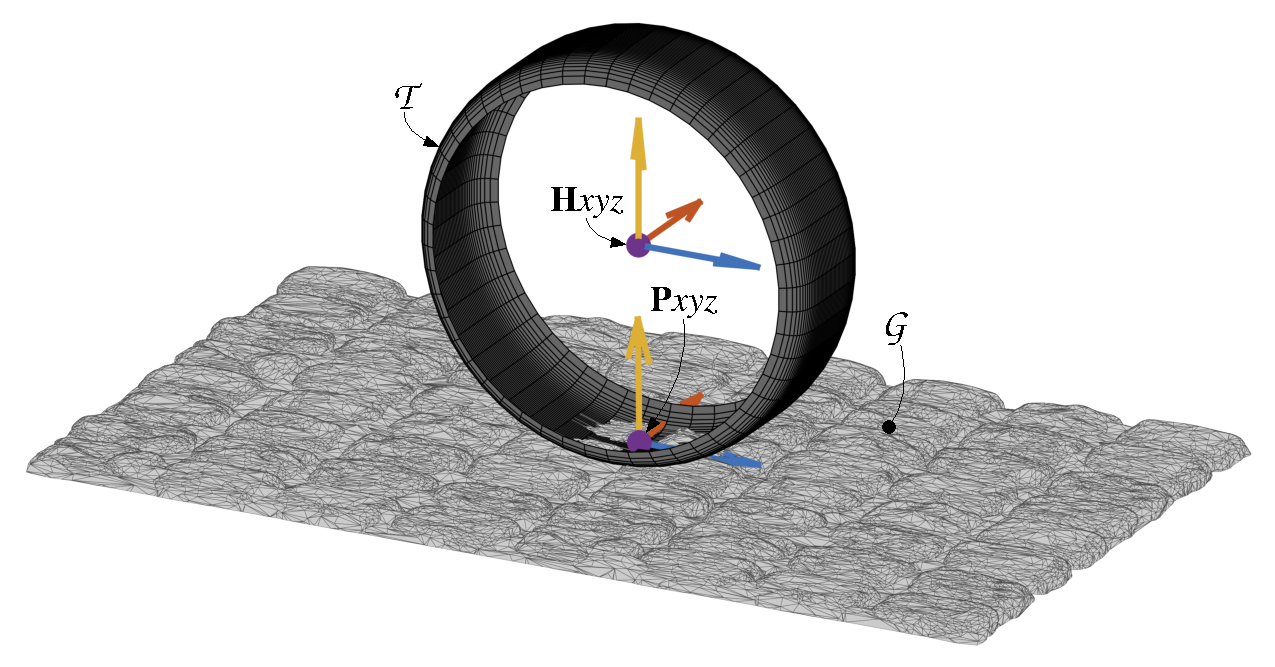
\includegraphics[width=1.0\textwidth, trim={5cm 2.3cm 5cm 0cm}, clip]{./figures/appendix_2/road_shell_ipe}
    \caption{Representation of the intersection between the tire $\sett{T}$ and a Belgian block road boundary $\sett{G}$ alongside the hub $\pt{H}xyz$ and the contact point $\pt{P}xyz$ reference frames.}
    \label{app2:fig:tire_shell}
  \end{subfigure}
  \hfill%
  \begin{subfigure}[t]{0.475\textwidth}
    \centering
    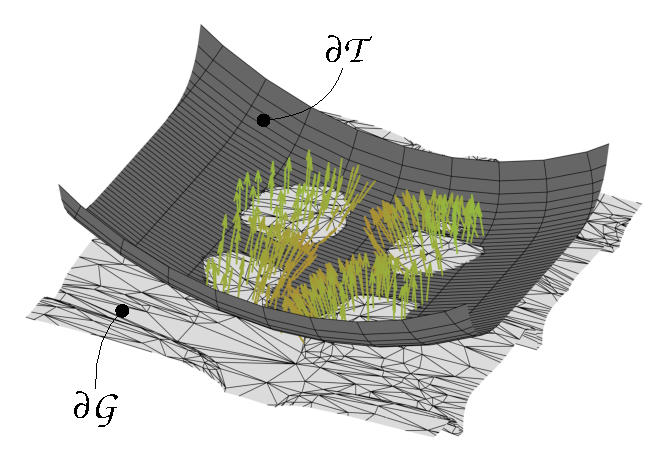
\includegraphics[width=1.0\textwidth]{./figures/appendix_2/zoom_ipe}
    \caption{Representation of the ground boundary $\boundary{G}$ normal directions (green arrows) inside the tire set boundary $\boundary{T}$. Each of these directions, together with other information, is exploited to calculate the contact point $\pt{P}$ and normal $\et{n}$.}
    \label{app2:fig:zoom}
  \end{subfigure}
  \caption{Representation of the tire-ground contact.}
  \label{app2:fig:tire_ground}
\end{figure}

To identify and quantify the contact between the tire and the ground we need to define what the intersection volume and the contact patch regions are. The intersection region is a closed set $\sett{V}$, collecting all the points of the tire $\sett{T}$, which are also points of the ground set $\sett{G}$, \ie{}, $\sett{V} = \sett{T} \cap \sett{G}$ (see Figure~\ref{app2:fig:zoom}). On the other hand, the contact patch is defined as a closed set $\sett{P}$ that collects all the points of the tire which are also interior points of the ground boundary surface $\boundary{G}$, \ie{}, $\sett{P} = \sett{T} \cap \boundary{G}$. The contact area $A$ and the contact volume $V$ are defined respectively as
%
\begin{center}
  \begin{minipage}[b]{0.425\textwidth}
    \vspace{-\baselineskip}
    \begin{equation}
      A = \iint_\sett{P} 1 \, \de\sett{\pt{x}}  \, \text{,}
      \label{app2:eq:int_area}
    \end{equation}
  \end{minipage}%
  \hfill\hfill and \hfill
  \begin{minipage}[b]{0.425\textwidth}
    \vspace{-\baselineskip}
    \begin{equation}
      V = \iiint_\sett{V} 1 \, \de\sett{\pt{x}} \, \text{.}
      \label{app2:eq:int_volume}
    \end{equation}
  \end{minipage}
\end{center}

The tire is assumed to be modeled by an infinite number of \emph{independent linear radial-springs}, whose stiffness $k$ is uniform all over the tire section. The inaccuracy introduced by this assumption is recovered by the tire force-calculation model, which employs concentrated parameters to describe the non-uniformity of the carcass stiffness. Before calculating the direction $\et{n}$ and application point $\pt{P}$ of the resultant contact force, we have to make three important observations.

\begin{observation}
  The force generated by the contact is produced by the deformation of the radial springs. If the terrain is non-deformable the contact force magnitude $\|\vt{F}\|$ is linearly proportional to the intersection volume $V$, \ie{},
  %
  \begin{equation*}
    \| \vt{F} \| = \iiint_\sett{V} k \, \de\sett{\pt{x}} = k V \propto V \, \text{.}
  \end{equation*}
  %
\end{observation}
%
Notice that the proportionality constant is the stiffness coefficient $k$, which is a function of the tire's internal structure and pressure. However, these dependencies are considered by the tire force-calculation model through lumped parameters. It should be pointed out that the damping effect is not considered due to the quasi-static nature of the enveloping phenomenon.
%
\begin{observation}
  Since the tire is assumed to be modeled by an infinite number of independent radial springs, the contact force $\vt{F}$ can not produce any rolling resistance torque around the wheel hub axis $\et{h}_y$. In other words, the contact force acts along the direction determined by one of the families of lines passing through the contact point $\pt{P}$ and the hub axis $\et{h}_y$.
\end{observation}
%
It is also important to note that the rolling resistance is not considered in the enveloping models. It is typically considered to be part of the tire contact force model, which must be fed with the information provided by the enveloping model. For instance, the \Swift{} model is coupled with the MagicFormulae{} model to compute the contact forces and torques generated by the tire-ground contact.

Thanks to these observations, the duality between the physical and geometrical models of the tire-ground contact can be exploited. Hence, the contact point $\pt{P}$ is calculated as the weighted average of contact surface points. The weight is proportional to the infinitesimal radial volume interested in the tire-ground contact. This infinitesimal radial volume is calculated as the intersection of the contact volume with the line $\ell(\pt{x},\et{h}_y)$ passing through the point $\pt{x} = [x, \, y, \, x]^\mathrm{T}$ and matching the axes of the wheel $\et{h}_y$ orthogonally. If $\mathrm{proj}(\pt{x},\boundary{G})$ defines the intersection point of the line $\ell(\pt{x},\et{h}_y)$ with $\boundary{G}$, then $\pt{P}$ is calculated as
%
\begin{equation}
  \pt{P} = \dfrac{1}{V} \displaystyle\iiint_\sett{V} \mathrm{proj}(\pt{x},\boundary{G}) \, \de\sett{\pt{x}}
  \, \text{.}
  \label{app2:eq:int_p}
\end{equation}
%
The application direction of the resultant tire-ground contact force is denoted by $\et{n}$. It is calculated as the average of the directions $\et{d}(\pt{x},\et{h}_y)$ of the lines $\ell(\pt{x},\et{h}_y)$, \ie{},
%
\begin{equation}
  \vt{n} = \displaystyle\iiint_\sett{V} \et{d}(\pt{x},\et{h}_y) \, \de\sett{\pt{x}},
  \quad \text{where} \quad
  \et{n} = \dfrac{\vt{n}}{\|\vt{n}\|}
  \, \text{.}
  \label{app2:eq:int_n}
\end{equation}
%
Similarly, the overall tire friction coefficient scaling factor $\lambda$ is calculated as
%
\begin{equation}
  \lambda = \dfrac{1}{V} \displaystyle\iiint_\sett{V} f(\pt{x}) \, \de\sett{\pt{x}}
  \, \text{.}
  \label{app2:eq:int_l}
\end{equation}
%
The solution of the here defined integrals~\eqref{app2:eq:int_p}, \eqref{app2:eq:int_n}, and~\eqref{app2:eq:int_l} is not straightforward. This is why, in the next section, we propose a numerical approximation of these integrals.

It should be pointed out that the local ground plane is hereafter identified by the reference frame $\pt{P}xyz$ whose origin point is $\pt{P}$ and axes directions are
%
\begin{equation*}
  \et{e}_z = \et{n} \, \text{,} \quad
  \et{e}_x = \dfrac{\et{h}_y \times \et{n}}{\|\et{h}_y \times \et{n}\|} \, \text{,} \quad \text{and} \quad
  \et{e}_y = \et{n} \times \et{e}_x
  \, \text{.}
\end{equation*}
%
The $\beta_x$ and $\beta_y$ angles, which are used to describe the local ground surface orientation with respect to the wheel hub, are calculated as the Euler angles ($zxy$ sequence) between the hub reference frame $\pt{H}xyz$ and the contact point reference frame $\pt{P}xyz$ (see Figure~\ref{app2:fig:tire_iso}).

\begin{figure}[htb]
  \centering
  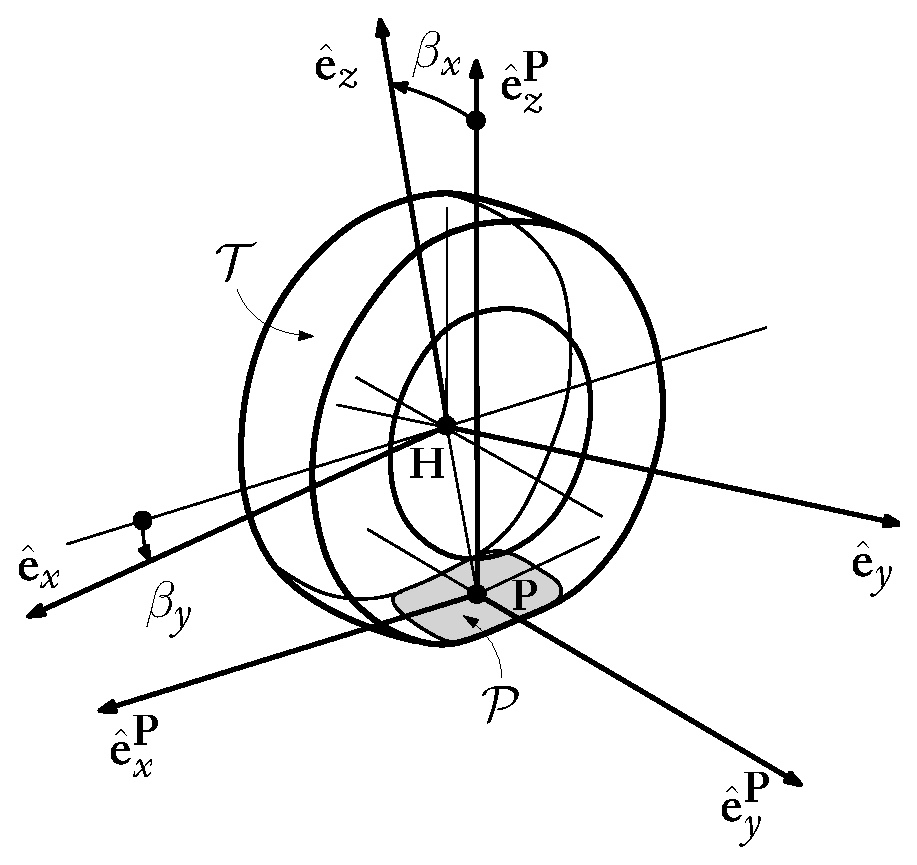
\includegraphics[width=9cm]{./figures/appendix_2/tire_iso}
  \caption{Representation of the contact pose $\pt{P}xyz$ along with the hub reference frame $\pt{H}xyz$ according to the ISO standard~\cite{iso88552011}. The constant pose is defined by the contact point $\pt{P}$ and the normal $\et{e}_z = \et{n}$, which also allows us to identify the forward and banking angles $\beta_x$ and $\beta_y$.}
  \label{app2:fig:tire_iso}
\end{figure}

% % % % % % % % % % % % % % % % % % % % % % % % % % % % % % % % % % % % % % % %

\section{Algorithm Implementation}
\label{app2:sec:algorithm_implementation}

So far, we have not yet described the actual shapes of the sets \sett{T} and \sett{G}, which represent the tire and the ground sets respectively. Since we will deal with complicated obstacle shapes it is important to restate the presented enveloping model in a formulation that does not limit its numerical efficiency, robustness, and scalability. For this reason, a discretized representation of tire and ground elements is required both to eventually solve the contact problem and to offer a highly scalable framework to work with. More specifically, the tire's external shape roughly corresponds to the external tread pattern profile revolved around the hub axis $\et{h}_y$. The tire set is discretized into a series of laterally lumped \emph{disks}, also called \emph{ribs}. On the other hand, the ground boundary is represented by a triangular mesh (see Figure~\ref{app2:fig:tire_zoom}). Both tire and ground descriptions are fully scalable as the density of the ribs and the triangles can be adjusted according to the accuracy and execution speed needed for the specific simulation. This representation approach turns out to be useful in the case of \ac{HRT} simulation (where the execution speed represents an important requirement that needs to be satisfied) but also in the case of offline simulations (where the demanded precision is usually higher).

\begin{figure}[htb]
  \centering
  \def\svgwidth{9cm}
  \input{./figures/appendix_2/tire_zoom.pdf_tex}
  \caption{Tire-road intersection with multiple instances of \Shell{} objects. Notice that the \Mesh{} is modeled as a multitude of \TriangleGround{} objects, while the \Shell{} object is made of a set of \Rib{}s. The \Rib{}s diameters and positions are extracted directly from the custom function $R(y)$ defined in the \Shape{} object.}
  \label{app2:fig:tire_zoom}
\end{figure}

The representation of tire and ground allows us to restate the enveloping model presented in Section~\ref{app2:sec:model} in a more ``software-friendly'' formulation. We will consider the discretized tire $\sett{S}$ as a set of $n$ tire ribs $\sett{\phi}$, \ie{}, $\sett{S} = \big\{ \sett{\phi}_1, \, \sett{\phi}_2, \, \dots \, \sett{\phi}_{n-1}, \, \sett{\phi}_{n}\big\}$. The generic tire rib $\sett{\phi}$ is defined geometrically as a disk of radius $r$, whose center is $\pt{O}$, and whose face normal corresponds to $\et{h}_y$. In addition, the rib also retains its ``virtual'' width $w \in \mathbb{R}_{\geq 0}$, which will be used in the numerical integration processes
%
\begin{equation}
  \sett{\phi} = \big\{ w \in \mathbb{R}_{\geq 0}, ~ \pt{x} = \left[x, y, z\right]^\mathrm{T} ~ \big\lvert ~ \pt{O} = \left[0, \, y, \, 0\right]^\mathrm{T}, r = R(y), ~ \|\pt{O} - \pt{x}\| \leq r, ~ \et{h}_y \cdot (\pt{O} - \pt{x}) = 0\big\} \, \text{.}
  \label{app2:eq:rib}
\end{equation}
%
Similarly, the discretized ground boundary $\boundary{G}$ is represented through a triangular mesh set $\sett{M}$ of $m$ triangles $\sett{\tau}$, \ie{}, $\sett{M} = \big\{ \sett{\tau}_1, \, \sett{\tau}_2, \, \dots, \, \sett{\tau}_{m-1}, \, \sett{\tau}_m \big\}$, where
%
\begin{equation}
  \begin{split}
    \begin{aligned}
      \sett{\tau} = \big\{ & \lambda\in\mathbb{R}_{\geq 0}, ~ \pt{x}\in\mathbb{R}^3 ~ \big\lvert ~ \pt{x} = t_1\,\pt{p}_1 + t_2\,\pt{p}_2 + t_3\,\pt{p}_3, ~ \dots \\
      &t_1 + t_2 + t_3 \leq 1, ~ t_1\geq 0, ~ t_2\geq 0, ~ t_3\geq 0\big\} \, \text{,}
    \end{aligned}
  \end{split}
  \label{app2:eq:triangleground}
\end{equation}
%
and where $\pt{p}_1$, $\pt{p}_2$, and $\pt{p}_3$ are the three vertices of the triangle. Notice that the mesh triangle $\sett{\tau}$ also carries a friction coefficient scaling factor $\lambda\in\mathbb{R}_{\geq 0}$, which is considered constant over the triangle surface.

The intersection between the set of ribs \sett{S} and the ground mesh triangles \sett{M} allows us to identify the contact parameters, namely the contact patch area $A$, the intersection volume $V$, the contact point location $\pt{P}$, and the contact force direction $\et{n}$. Trivially, if a generic rib $\sett{\phi}$ is intersected with a generic mesh triangle $\sett{\tau}$, the result will be a set $\sett{\sigma} = \sett{\phi} \cap \sett{\tau}$. This intersection can lead to four different cases, in which the set $\sett{\sigma}$ can be: (1) an empty set, if $\sett{\phi}$ does not touch $\sett{\tau}$ at all; (2) a point, if $\sett{\phi}$ intersects $\sett{\tau}$ one of its vertices; (3) a segment, if $\sett{\phi}$ intersects $\sett{\tau}$ or a portion of it; and (4) a convex hull, if $\sett{\phi}$ and $\sett{\tau}$ are coplanar and intersect. Cases 1 and 2 are not considered since they are not relevant to the modeled contact. Case 4 corresponds to a tire lying on the ground, which is not relevant for a vehicle simulation in which the tire is always rolling. Hence, case 3 is the only relevant one for the modeled contact. In this case, the intersection region is a segment $\sett{\sigma}$ such that
%
\begin{equation*}
  \sett{\sigma} = \big\{ \pt{x}\in\mathbb{R}^3 ~ \big\lvert ~ \pt{x}=(1-t)\,\pt{p}_a + t\,\pt{p}_b, ~ t \in [0, \, 1] \big\}
   \, \text{,}
\end{equation*}
%
where $\pt{p}_a$ and $\pt{p}_b$ are the two extrema points of the segment. We can now calculate the contact patch area $A$ by restating~\eqref{app2:eq:int_area} as the summation
%
\begin{equation}
  A = \sum_{i=1}^{n} w_i \sum_{j=1}^{m} \left\|\pt{p}_{b,ij} - \pt{p}_{a,ij}\right\|_{2}
   \, \text{,}
  \label{app2:eq:int_a_crt}
\end{equation}
%
where $w_i$ is the ``virtual'' width of the $i$-th rib.

To solve integrals~\eqref{app2:eq:int_volume}, \eqref{app2:eq:int_p} and~\eqref{app2:eq:int_n}, they are first transformed to cylindrical coordinates. Moreover, $\bar{\sett{\sigma}}$ denotes the transformation to into cylindrical coordinates of $\sett{\sigma}$. The radius $\bar{r}(\theta)$ represents the distance from the rib center point $\pt{O}$ to a generic point of the intersection segment $\bar{\sett{\sigma}}$. Denote with $r_i$ the radius of the $i$-th rib and with $\bar{r}_{ij}(\theta)$ the distance between the $i$-th rib center point and the segment $\bar{\sett{\sigma}}_{ij}$; where the segment $\bar{\sett{\sigma}}_{ij}$ is identified as the intersection of the $i$-th rib with the $j$-th triangle. The range of the angle $\theta$ for the generic segment $\bar{\sett{\sigma}}$ is denoted with $[\theta^a,\theta^b]\subset (\pi,2\pi)$, which are implicitly defined as
%
\begin{equation*}
  \begin{bmatrix} \cos \theta^a \\ \sin \theta^a \end{bmatrix}=
  \dfrac{\pt{p}_a - \pt{O}}{\|\pt{p}_a - \pt{O}\|}
   \, \text{,} \quad \text{and} \quad
  \begin{bmatrix} \cos \theta^b \\ \sin \theta^b \end{bmatrix}=
  \dfrac{\pt{p}_b - \pt{O}}{\|\pt{p}_b - \pt{O}\|}
  \, \text{.}
\end{equation*}
%
With this notation the integrals~\eqref{app2:eq:int_volume}, \eqref{app2:eq:int_p}, \eqref{app2:eq:int_n} and~\eqref{app2:eq:int_l} are rewritten as
%
\begin{equation}
  v_{ij}(\theta) = \dfrac{r_i^2-\bar{r}_{ij}(\theta)^2}{2}
   \, \text{,}
  \label{app2:eq:int_v_ij}
\end{equation}
%
\begin{equation}
  V = \sum_{i=1}^{n}w_i \sum_{j=1}^{m} \int_{\theta^a_{ij}}^{\theta^b_{ij}} v_{ij}(\theta) \, \de\theta
   \, \text{,}
  \label{app2:eq:int_v_cyl}
\end{equation}
%
\begin{equation}
  \pt{P} =
    \dfrac{1}{V} \sum_{i=1}^{n}w_i\sum_{j=1}^{m} \displaystyle\int_{\theta^a_{ij}}^{\theta^b_{ij}}
  \begin{bmatrix}
    \bar{r}_{ij}(\theta)\cos(\theta)v_{ij}(\theta)
    \\[2mm]
    y_i v_{ij}(\theta)
    \\[2mm]
    \bar{r}_{ij}(\theta)\sin(\theta)v_{ij}(\theta)
  \end{bmatrix} \, \de\theta
   \, \text{,}
  \label{app2:eq:int_p_cyl}
\end{equation}
%
\begin{equation}
  \vt{n} =
  \sum_{i=1}^{n}w_i\sum_{j=1}^{m} \displaystyle\int_{\theta^a_{ij}}^{\theta^b_{ij}}
  \begin{bmatrix}
    \cos(\theta)v_{ij}(\theta)
    \\[2mm]
    0
    \\[2mm]
    \sin(\theta)v_{ij}(\theta)
  \end{bmatrix} \, \de\theta  \, \text{,} \quad
  \et{n} = \dfrac{\vt{n}}{\|\vt{n}\|}
   \, \text{,}
  \label{app2:eq:int_n_cyl}
\end{equation}
%
\begin{equation}
  \lambda = \dfrac{1}{V} \sum_{i=1}^{n}w_i\sum_{j=1}^{m} \int_{\theta^a_{ij}}^{\theta^b_{ij}} \lambda v_{ij}(\theta) \, \de\theta
  \, \text{.}
  \label{app2:eq:int_l_cyl}
\end{equation}
%
Notice that the intermediate variable $v_{ij}(\theta)$ in~\eqref{app2:eq:int_v_ij} represents the length of the generic segment radially connecting the $\bar{\sett{\sigma}}_{ij}$ to the external tire boundary at the angle $\theta$ (see~Figure~\ref{app2:fig:intersection}). From a physical perspective, $v_{ij}(\theta)$ is the deflection of the infinitesimal radial springs at the angle $\theta$. It is possible to find a closed-form solution for $\bar{r}_{ij}(\theta)$. However, the analytical expression of the resulting $\pt{P}$ and $\et{n}$ is excessively long. For practical purposes, it is better to use a quadrature formula to numerically approximate the integrals. In this work, Simpson's $1/3$ rule is used.
%
\begin{remark}
  Simpson's $1/3$ rule quadrature formula of $f(x)$ for the interval $[a,b]$ reads as
  %
  \begin{equation*}
    \int_{a}^b f(x)\,\de x = \dfrac{h}{6}\left[ f(a) + 4f\left(c\right)+f(b)\right] - \dfrac{h^5}{2880} f^{(4)}(\xi)
     \, \text{,}
  \end{equation*}
  %
  where $h = b-a$, $c = (a+b)/2$, and $\xi \in [a, \, b]$~\cite{stoer2002introduction}. Notice that if $r \leq 1$, $\theta^b-\theta^a \leq \pi/6$, and $1 \geq \|\pt{O}-\pt{p}_{a,b}\| \geq 4/5$, the relative error of the numerically computed integrals in~\eqref{app2:eq:int_v_cyl}, \eqref{app2:eq:int_p_cyl}, and~\eqref{app2:eq:int_n_cyl} is below $1\%$.
\end{remark}
%
\begin{remark}
  The midpoint $\bar{r}((\theta^a+\theta^b)/2)$ is computed as
  %
  \begin{equation*}
    \bar{r}\bigg(\dfrac{\theta^b-\theta^a}{2}\bigg) = \dfrac{2\bar{r}(\theta^a)\bar{r}(\theta^b)}{\bar{r}(\theta^a)+\bar{r}(\theta^b)}\cos\bigg(\dfrac{\theta^b-\theta^a}{2}\bigg)
    \, \text{.}
  \end{equation*}
\end{remark}

\begin{figure}[htb]
  \centering
  \def\svgwidth{9cm}
  \input{./figures/appendix_2/intersection.pdf_tex}
  \caption{Representation of the intersection between a tire rib $\sett{\phi}$ (\textcolor[RGB]{255, 231, 187}{$\blacksquare$}) and a ground mesh triangle $\sett{\tau}$ (\textcolor[RGB]{255, 218, 217}{$\blacksquare$}). The intersection set $\sigma$ (\textcolor[RGB]{74, 181, 99}{$\blacksquare$}) is a segment with
  vertices $\pt{p}_a$ and $\pt{p}_b$, at $\theta^a$ and $\theta^b$ angles respectively.}
  \label{app2:fig:intersection}
\end{figure}

% % % % % % % % % % % % % % % % % % % % % % % % % % % % % % % % % % % % % % % %

\section{Software Architecture}
\label{app2:sec:software_architecture}

The \Enve{} algorithm-based software is written in \cpp{} (2011 standard~\cite{stroustrup2013cpp}), which is one of the most widely supported, common and fast among object-oriented general-purpose programming languages. We have only reduced the dependencies on the \Eigen{}~\cite{eigen2010eigen} and \Acme{}~\cite{stocco2021acme} libraries: this provides us with a flexible and extensible framework. \Eigen{} is a template library for linear algebra. It is very efficient for small vectors and matrices and can exploit \ac{LAPACK}/\ac{BLAS}~\cite{anderson1999lapack} for peak performance when matrices and vectors have a large size. \Acme{}, on the other hand, is an easy-to-use geometry library that aims to be a minimal tool for \ac{HRT} scheduling applications. Furthermore, \Matlab{}~\Mex{} and \Simulink{}~\SFunction{} extensions are provided to allow the integration of \Enve{} in more complex simulation environments. The software is distributed under the BSD 3-Clause License and is freely available online~\cite{enve}.

\subsection{Data Types}
\label{app2:sec:data_types}

The software is built on a limited number of classes. We have chosen to keep the library as essential as possible for ease of maintenance and efficiency. For this reason, we use the necessary classes to describe and manipulate virtual ground surfaces and tires. Each geometrical entity representing the tire and ground is organized in a specific class. A brief description of the data types used in the software is now given in this section.

\paragraph{\TriangleGround{}}
The generic ground triangle $\sett{\tau}$ is defined by the three points $\pt{p}_1$, $\pt{p}_2$ and $\pt{p}_3$. In this way, it geometrically corresponds to the \Triangle{} object described in the \Acme{} library~\cite{stocco2021acme}. For this reason, the \TriangleGround{} object publicly inherits from the \Acme{}::\Triangle{} object. Since the \TriangleGround{} object describes the generic triangle representing a local road region, this class also carries a scaling factor for the friction coefficient $\lambda$. The mathematical representation corresponds to the definition in~\eqref{app2:eq:triangleground}.

\paragraph{\Mesh{}}
The mesh represents the discretized ground set $\sett{M}$ on which the tire rolls. It is composed of a multitude of \TriangleGround{} objects. The size of these triangles is determined according to end-use requirements and desired accuracy. As a consequence, the number of triangles can range from a few dozen to tens of thousands. For this reason, the \Acme{} library's \AabbTree{} data structure is used to efficiently manage the intersection between the tire and the ground, and substantial acceleration of the overall algorithm is achieved.

\paragraph{\Flat{}}
Using a mesh to represent a flat ground surface is not always the most efficient choice, as this can prolong the time needed for computation unnecessarily. With a \Mesh{} the software is forced to go through the creation of an \AabbTree{} and to make an evaluation of the intersection of the same tree with the \Aabb{} containing the tire. To eliminate this source of inefficiency, the \Flat{} class has been implemented, to represent a perfectly flat terrain. The \Flat{} object publicly inherit from the \Acme{}::\Plane{} object and a friction coefficient scaling factor $\lambda$ is added to the class description
%
\begin{equation*}
  \sett{\pi} = \big\{ \lambda \in \mathbb{R}_{\geq 0}, ~ \pt{x},\pt{p},\et{n} \in \mathbb{R}^3 ~ \big\lvert ~ \et{n} \cdot (\pt{p} - \pt{x}) = 0\big\}
   \, \text{,}
\end{equation*}
%
where $\pt{p}$ is a generic point on the plane and $\et{n}$ is a unit normal vector.

\paragraph{\Shape{}}
The \Shape{} object describes the overall external shape of the tire $\sett{T}$ and of all the ribs in the set $\sett{S}$. The external boundary of the tire $\boundary{T}$ is defined as a surface generated by the revolution of an arbitrary function $R(y)$. By using the proper surface of revolution, it is possible to represent a wide variety of tire morphologies, ranging from car tires to motorcycle tires (see Figure~\ref{app2:fig:tire_shell}).

\paragraph{\Rib{}}
As mentioned before, the rib is considered a small section of the overall tire. Geometrically the rib is defined as a disk $\sett{\phi}$ of radius $r$, whose center $\pt{O}$ is located in $[0, \, y, \, 0]^\mathrm{T}$ in the $\pt{H}xyz$ wheel hub reference frame and whose lateral coordinate $y$ is constant throughout the whole disk area. The~\Rib{} object publicly inherit from the \Acme{}::\Disk{} object. In addition, the~\Rib{} class also carries its ``virtual'' width $w \in \mathbb{R}_{\geq 0}$, which is stored as a class member. The mathematical representation of this set corresponds to that in~\eqref{app2:eq:rib}.

\paragraph{\Shell{}}
The shell object encapsulates the set of~\Rib{} objects $\sett{S}$, along with a shared pointer to a \Shape{} object and an object of the type \Acme{}::\Aabb{}. This last object represents the bounding box that contains the tire at every instant of time. The \Shell{} object also contains all the attributes and secondary objects that are used to describe the tire and its intersection with the terrain. Whenever an intersection between the tire and the terrain occurs, the affine transformation describing the tire pose as well as the tire \Aabb{} is updated. Once these basic operations are completed, the bounding box is intersected with the \Acme{}::\AabbTree{} of the mesh. A list of shared pointers to \TriangleGround{} objects that are internal or that simply touch the tire bounding box is generated. This list is supplied one by one to the~\Rib{} objects to find the intersection parameters described in the previous section. To avoid unnecessary recalculations, the intersection parameters are stored in members that are internal to the \Shell{} class; they are then eventually extracted with methods specifically designed for this purpose.

\subsection{Algorithm Workflow}
\label{app2:sec:algorithm_workflow}

The workflow of the algorithm is highly streamlined. It is divided into three main algorithms that are briefly described below briefly described and that are also reported in the pseudocodes. Other minor algorithms are used to support the main ones and are not reported here for the sake of brevity.

\paragraph{Shell Initialization}
The initialization of the \Shell{} object is done by passing a \Shape{} object and the number of ribs $n$ as input parameters. Firstly, the \Shape{} object is used to reconstruct the tire's external shape; then the \Rib{} objects are instantiated by discretizing the tire into $n$ ribs.

\begin{breakablealgorithm}
  \caption{Initialization of a \Shell{} object.}
  \label{app2:alg:shell}
  \begin{algorithmic}[1]
    \State \textbf{Require:} The tire \Shape{} object, and the number of ribs $n$
    \Function{\Shell{}}{$\Shape{}, \, n$} \Comment{\Shell{} class constructor}
      \State $\sett{S} \gets \varnothing$ \Comment{Initialize the set of ribs}
      \State $w \gets \Shape{}.\text{width}()/n$ \Comment{The ribs width}
      \For{$i \gets 1$ to $n$}
        \State $y_i \gets w/2 + (i-1)\,w$ \Comment{The $i$-th rib lateral coordinate}
        \State $r_i \gets \Shape{}.\text{radius}(y_i)$ \Comment{The $i$-th rib radius}
        \State $\sett{S}_i \gets \Rib{}(r_i, \, y_i, \, w)$ \Comment{The $i$-th rib}
      \EndFor
      \State $F \gets \mathbf{I}_{4 \times 4}$ \Comment{The default affine transformation}
      \State $B \gets \Aabb{}(\sett{S}, F)$ \Comment{The bounding box of the tire}
      \State \textbf{store} $\sett{S}, \, B, \, F$ \Comment{Store the data in class members}
      \EndFunction
  \end{algorithmic}
\end{breakablealgorithm}

\paragraph{Mesh Initialization}
The \Mesh{} object is initialized by passing a Road Data Format or Wavefront OBJ extension file containing the triangles' vertices and faces as input. The file is first parsed to instantiate the mesh \TriangleGround{} objects and then used to build the \AabbTree{}, which will later be used to accelerate the intersection process as well as the calculation of contact parameters.

\begin{breakablealgorithm}
  \caption{Initialization of a \Mesh{} object.}
  \label{app2:alg:mesh}
  \begin{algorithmic}[1]
    \State \textbf{Require:} The mesh file path
    \Function{Mesh}{$\text{path}$} \Comment{\Mesh{} class constructor}
      \State $V \gets \varnothing$ \Comment{Initialize ground mesh vertices}
      \State $F \gets \varnothing$ \Comment{Initialize mesh faces}
      \State $\lambda \gets \varnothing$ \Comment{Initialize mesh $\lambda$s}
      \State $V, \, F, \, \lambda \gets \Mesh{}.\text{parse}(\text{file})$ \Comment{Parse the mesh file}
      \State $\sett{M} \gets \varnothing$ \Comment{Initialize the set of triangles}
      \State $B \gets \varnothing$ \Comment{Initialize the set of triangles' \Aabb{}s}
      \State $n \gets F.\text{size}()$ \Comment{The number of triangles}
      \For{$i \gets 1$ to $n$}
        \State $\pt{p}_1 \gets V(F(i,1))$ \Comment{The 1\textsuperscript{st} triangle vertex}
        \State $\pt{p}_2 \gets V(F(i,2))$ \Comment{The 2\textsuperscript{nd} triangle vertex}
        \State $\pt{p}_3 \gets V(F(i,3))$ \Comment{The 3\textsuperscript{rd} triangle vertex}
        \State $\sett{M}_i \gets \TriangleGround{}(\pt{p}_1, \, \pt{p}_2, \, \pt{p}_3, \, \lambda(i))$ %\Comment{The $i$-th triangle object}
        \State $B_i \gets \Aabb{}(\sett{M}_i)$ \Comment{The $i$-th triangle \Aabb{}}
      \EndFor
      \State $T \gets \AabbTree{}(\sett{M}, \, B)$ \Comment{The mesh's \AabbTree{}}
      \State \textbf{store} $\sett{M}, \, T$ \Comment{Store the data in class members}
    \EndFunction
  \end{algorithmic}
\end{breakablealgorithm}

\paragraph{Contact Parameters Calculation}
The contact parameters are calculated by intersecting the \Shell{} object and the \Mesh{} object. This is done by calling the ``setup'' method of the \Shell{} object. Firstly, this method intersects the mesh's \AabbTree{} with the tire's \Aabb{} and returns a list of triangles that are potentially intersecting the tire. Then, the tire ribs are intersected with the triangles and the contact parameters are calculated as described in Section~\ref{app2:sec:model}.

\begin{breakablealgorithm}
  \caption{Contact parameters calculation.}
  \label{app2:alg:intersection}
  \begin{algorithmic}[1]
    \State \textbf{Require:} The new tire affine transformation $F$, and the \Mesh{} object $\sett{M}$
    \Function{\Shell{}{\normalfont.setup}}{$F, \, \sett{M}$} \Comment{The intersection method}
      \State $B \gets \Shell{}.\text{update\_aabb}(F)$ \Comment{Update the tire \Aabb{}}
      \State $L \gets \Mesh{}.\text{intersect}(B)$ \Comment{The intersecting triangles}
      \State $r \gets \sett{S}.\text{size}()$ \Comment{The number of tire ribs}
      \State $n \gets L.\text{size}()$ \Comment{The number of intersecting triangles}
      \State $A \gets 0$ \Comment{Initialize the contact patch area}
      \State $V \gets 0$ \Comment{Initialize the intersection volume}
      \State $\pt{P} \gets \pt{0}$ \Comment{Initialize the contact point}
      \State $\et{n} \gets \pt{0}$ \Comment{Initialize the contact normal}
      \State $\lambda \gets 0$ \Comment{Initialize the friction coefficient scaling factor}
      \For{$i \gets 1$ to $r$}
        \For{$j \gets 1$ to $n$}
          \State $\sigma \gets \sett{S}_i \cap \sett{M}_{L(j)}$ \Comment{The intersection set (segment)}
          \State $A \gets A + \sett{\sigma}.\text{area}()$ \Comment{The contact area~\eqref{app2:eq:int_a_crt}}
          \State $V \gets V + \sett{\sigma}.\text{volume}()$ \Comment{The contact volume~\eqref{app2:eq:int_v_cyl}}
          \State $\pt{P} \gets \pt{P} + \sett{\sigma}.\text{point}()$ \Comment{The contact point~\eqref{app2:eq:int_p_cyl}}
          \State $\et{n} \gets \et{n} + \sett{\sigma}.\text{normal}()$ \Comment{The contact normal~\eqref{app2:eq:int_n_cyl}}
          \State $\lambda \gets \lambda + \sett{\sigma}.\text{lambda}()$ \Comment{The contact $\lambda$~\eqref{app2:eq:int_l_cyl}}
          \EndFor
      \EndFor
      \State $\lambda \gets \lambda/V$ \Comment{The average $\lambda$}
      \State \textbf{return} $A, \, V, \, \pt{P}, \, \et{n}, \, \lambda$ \Comment{The contact parameters}
    \EndFunction
  \end{algorithmic}
\end{breakablealgorithm}

% % % % % % % % % % % % % % % % % % % % % % % % % % % % % % % % % % % % % % % %

\section{Simulations and Discussion}
\label{app2:sec:discusson}

In this section, we present some simulations to prove the capabilities of the proposed model. The simulations are divided into two categories: quasi-static simulations, and \ac{RT} performance assessments. Quasi-static simulations are carried out according to the SAE J2731 standard~\cite{saej2731} to assess the enveloping capabilities at low speed of the presented model, while dynamic simulations highlight the outcomes of the tire-ground enveloping model in a dynamic scenario. In both types of simulations, a comparison with the \Swift{} model~\cite{schmeitz2004semiempirical} and the \TMEasy{} model~\cite{rill2018sophisticated} is provided. Simulations are performed by modeling the tire as a 205/60R15 (\SSI{2.2}{\bar} inflation pressure) passenger car tire, which is one of the tires used in~\cite{schmeitz2004semiempirical} to validate the \Swift{} model. The tire is discretized into 10 $\times$ 10 cams for the \Swift{} model and 10 ribs for the \Enve{} model.

\subsection{Quasi-Static Simulations on Uneven Road Surfaces}
\label{app2:sec:enveloping}

As mentioned before the aim of the first set of simulations is to assess the enveloping capabilities of the presented model at a low speed according to SAE J2731 standard~\cite{saej2731}. As motivated in the SAE standard, we want to assess under quasi-static considerations the ability of the model to correctly estimate the contact point height $z$\footnote{The contact point height is defined as the $z$-axis component of the contact point position $\pt{P}$ in the absolute reference frame.} and the forward and lateral slope angles $\beta_x$ and $\beta_y$ respectively. In this regard, we have considered three different road surfaces, characterized by different degrees of unevenness. On each of these surfaces, we have performed a set of simulations with constant vertical loads $F_z$ of 2, 4 and \SSI{6}{\kilo\newton}. It must be pointed out that the \TMEasy{} model output does not change with the vertical load $F_z$ and is thus reported with a single line in the plots.

The first simulation is performed on a series of different obstacles positioned orthogonally to the forward direction of the tire. Specifically, the obstacles' cross-sections are depicted at the top of~Figure~\ref{app2:fig:steps}. The results of the simulation are reported in the last two plots of~Figure~\ref{app2:fig:steps}. As it can be noticed, the behavior of the presented model is similar to that of the \Swift{} model, which is considered to be very close to the ground truth (see~\cite{schmeitz2004semiempirical} for an in-depth discussion on the \Swift{} model and its accuracy). The performance of \Enve{} depends on the geometry of the obstacles. Indeed, in the presented model the contact parameters are defined only by the geometry of the obstacles, which is not entirely true in the real world. Tire nonlinear radial stiffness and inflation pressure also play a non-negligible role in defining the overall tire-ground contact behavior. However, given the simplicity of the model, the results are quite satisfactory. Conversely, the \TMEasy{} model does not produce realistic results, causing abrupt changes in the contact parameters: $z$, $\beta_x$, and $\beta_y$.

The last simulation is performed on a rough Belgian block road surface depicted in~Figure~\ref{app2:fig:tire_shell}. The results reported in~Figure~\ref{app2:fig:cobblestone}, show that the \Enve{} model behavior is very close to that of the \Swift{} model in terms of contact point height $z$ and forward slope angle $\beta_y$. However, the \Enve{} model is not able to correctly estimate the lateral slope angle $\beta_x$. Even on the rough Belgian block road surface, the \TMEasy{} model is unable to correctly estimate the contact point height $z$ and the lateral slope angle $\beta_x$. Moreover, it strongly overestimates the forward slope angle $\beta_y$.

\begin{figure}[htb]
  \centering
  \hspace{1.5cm}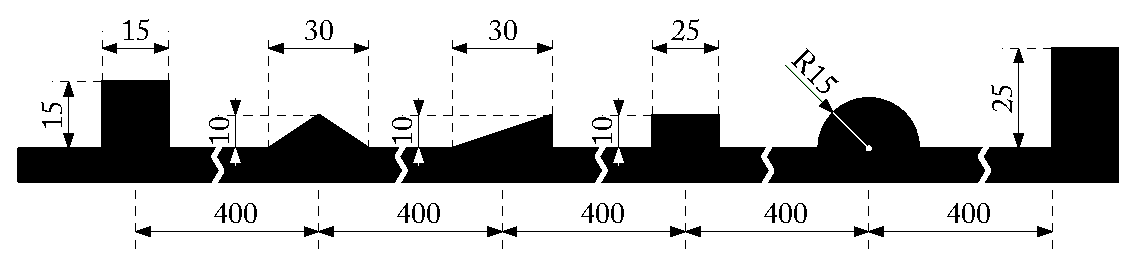
\includegraphics[width=9.0cm]{./figures/appendix_2/steps_ipe}\\[0.1in]
  \small{\includetikz{figures/appendix_2/steps.tex}}
  \caption{Quasi-static simulations of a 205/60R15 tire rolling over a stepped road surface. The \TMEasy{} model output does not change with the vertical load $F_z$ and is reported with a single line. \emph{Colors legend}: {\color{mycolor1}$\blacksquare$}~$F_z =$ \SSI{2}{\kilo\newton}, {\color{mycolor2}$\blacksquare$}~$F_z =$ \SSI{4}{\kilo\newton}, and {\color{mycolor3}$\blacksquare$}~$F_z =$ \SSI{6}{\kilo\newton}. \emph{Lines legend}: \raisebox{1.0pt}{\textbf{---}}~\Enve{}, \raisebox{1.0pt}{\textbf{--~--}}~\Swift{}, and {\color{mycolor5}$\blacksquare$}~\TMEasy{}, and {\color{black}$\blacksquare$}~road surface cross-section.}
  \label{app2:fig:steps}
\end{figure}

\begin{figure}[htb]
  \centering
  \small{\includetikz{figures/appendix_2/cobblestone.tex}}
  \caption{Quasi-static simulations of a 205/60R15 tire rolling over a Belgian block road surface. The \TMEasy{} model output does not change with the vertical load $F_z$ and is reported with a single line. \emph{Colors legend}: {\color{mycolor1}$\blacksquare$}~$F_z =$ \SSI{2}{\kilo\newton}, {\color{mycolor2}$\blacksquare$}~$F_z =$ \SSI{4}{\kilo\newton}, and {\color{mycolor3}$\blacksquare$}~$F_z =$ \SSI{6}{\kilo\newton}. \emph{Lines legend}: \raisebox{1.0pt}{\textbf{---}}~\Enve{}, \raisebox{1.0pt}{\textbf{--~--}}~\Swift{}, and {\color{mycolor5}$\blacksquare$}~\TMEasy{}, and {\color{black}$\blacksquare$}~road surface cross-section.}
  \label{app2:fig:cobblestone}
\end{figure}

% % % % % % % % % % % % % % % % % % % % % % % % % % % % % % % % % % % % % % % %

\subsection{Full-Vehicle Model Simulation}
\label{app2:sec:simulator}

To evaluate the behavior of the presented tire-ground enveloping model in a typical use case, it is integrated into a complete \ac{RT} vehicle simulation framework, and compared with the \Swift{}~\cite{schmeitz2004semiempirical} and \TMEasy~\cite{rill2013tmeasy, rill2018sophisticated}{} enveloping models. The used framework consists of a DIL/SIL/HIL simulator based on a custom high-fidelity vehicle model. Vehicle dynamics is described by a 14 \acp{DOF} full-vehicle model able to accurately simulate the impact of suspension kinematics and compliance on vehicle behavior within the typical range of frequencies for the ride and handling analysis. Contrary to widespread practice, the vehicle dynamic equations are not linearized. This improves model accuracy in nonlinear regions and vehicle attitude even in abnormal conditions. The described formulation enables the vehicle model for 3D road simulations. It is worth noting that additional \acp{DOF} are used to describe internal components' dynamics, such as the powertrain, the steering system or the tire subsystems. The structure of the model is organized in a modular fashion mirroring the mechanical interfaces of vehicle components. This modular structure makes the integration of third-party software or, more generally, of any external system a fairly straightforward process. As a result, it is possible to easily configure the vehicle model for HIL, SIL and/or DIL simulations. The developed enveloping model is thus interfaced, as a subsystem with the vehicle\ac{MB} system through a pre-defined model interface. Inputs of the tire-ground contact subsystem are the wheels' reference frames as well as the wheels' geometrical characteristics and the 3D road surface mesh. The outputs of the subsystem are, for each wheel, the equivalent tire contact point, the local contact plane, the contact penetration and the local friction coefficient. Road contact parameters, extracted from the tire-ground enveloping model, are then used by the \MagicFormulae{}~6.2 tire model to compute contact forces.

The modeled vehicle is a passenger car with sedan-like characteristics. The vehicle features a fully electric powertrain with a front-wheel drive transmission layout. The modeled suspensions are a MacPherson configuration for the front suspensions and a Multi-Link scheme for the rear suspensions. For the sake of brevity, only the most relevant vehicle parameters are listed in \tablename~\ref{app2:tab:vehicle_data}.

\begin{table}[htb]
  \centering
  \begin{tabular}{lc}
    \toprule
    \textbf{Parameter description}              & \textbf{Value} \\
    \midrule
    Total mass of the vehicle                   & \SSI{1300}{\kilo\gram} \\
    Center-of-mass height                       & \SSI{0.30}{\meter} \\
    Front axle distance from the center-of-mass & \SSI{1.25}{\meter} \\
    Rear axle distance from the center-of-mass  & \SSI{1.45}{\meter} \\
    Wheelbase                                   & \SSI{2.70}{\meter} \\
    Yaw inertia                                 & \SSI{1400}{\kilo\gram\meter\squared} \\
    Track width                                 & \SSI{1.50}{\meter} \\
    Steering ratio                              & \num{20} \\
    Maximum torque at wheel                     & \SSI{1200}{\newton\meter} \\
    Maximum motor power                         & \SSI{150}{\kilo\watt} \\
    Wheel inertia around rotation axis          & \SSI{1.40}{\kilo\gram\meter\squared} \\
    Size specification of the tires             & \num{205}/\num{60}R\num{15} \\
    Spring stiffness at wheel                   & \SSI{3530}{\kilo\newton\per\meter} \\
    Damping coefficients at wheel for jounce    & \SSI{789}{\newton\second\per\meter} \\
    Damping coefficients at wheel for rebound   & \SSI{1578}{\newton\second\per\meter} \\
    \bottomrule
  \end{tabular}
  \caption{Main parameters of the modeled vehicle.}
  \label{app2:tab:vehicle_data}
\end{table}

\begin{figure}[htb]
  \centering
  \small{\includetikz{figures/appendix_2/accelerations.tex}}
  \caption{Chassis accelerations of the full-vehicle model driving over a \SSI{45}{\deg} oblique step of \SSI{1}{\centi\meter} at a longitudinal speed of \SSI{10}{\kilo\meter\per\hour}. \emph{Legend}:
  {\color{mycolor1}$\blacksquare$}~\Enve{}, {\color{mycolor2}$\blacksquare$}~\Swift{}, and {\color{mycolor3}$\blacksquare$}~\TMEasy{}.}
  \label{app2:fig:accelerations}
\end{figure}

\begin{figure}[htb]
  \centering
  \small{\includetikz{figures/appendix_2/forces.tex}}
  \caption{Front-left tire forces of the full-vehicle model driving over a \SSI{45}{\deg} oblique step of \SSI{1}{\centi\meter} at a longitudinal speed of \SSI{10}{\kilo\meter\per\hour}. \emph{Legend}: {\color{mycolor1}$\blacksquare$}~\Enve{}, {\color{mycolor2}$\blacksquare$}~\Swift{}, and {\color{mycolor3}$\blacksquare$}~\TMEasy{}.}
  \label{app2:fig:forces}
\end{figure}

\begin{figure}[htb]
  \centering
  \small{\includetikz{figures/appendix_2/rhos.tex}}
  \caption{Tires deflections of the full-vehicle model driving over a \SSI{45}{\deg} oblique step of \SSI{1}{\centi\meter} at a longitudinal speed of \SSI{10}{\kilo\meter\per\hour}. \emph{Legend}: {\color{mycolor1}$\blacksquare$}~\Enve{}, {\color{mycolor2}$\blacksquare$}~\Swift{}, and {\color{mycolor3}$\blacksquare$}~\TMEasy{}.}
  \label{app2:fig:rho}
\end{figure}

Model accuracy and robustness are widely tested with DIL simulations by driving the vehicle in urban scenarios, characterized by speed bumps, sidewalks or, generally, uneven road surfaces. In this work, we present the results obtained by driving the vehicle at a longitudinal speed of \SSI{10}{\kilo\meter\per\hour} over a \SSI{45}{\deg} oblique and \SSI{1}{\centi\meter} high step. The reported results are the chassis accelerations (Figure~\ref{app2:fig:accelerations}), front-left tire forces (Figure~\ref{app2:fig:forces}), and the tires deflections (Figure~\ref{app2:fig:rho}). Note that \Enve{} and \Swift{} enveloping models present a similar behavior even in the case of a simulation of a full-vehicle model. In fact, the generated chassis accelerations, the tires' forces, and deflections are in agreement with each other. The discontinuities in both the contact point height and the banking and forward slope angles of the \TMEasy{} model reflect on the full-vehicle model simulations with abrupt changes contact forces as well as chassis acceleration not seen in experimental measurements. Notice that according to the results reported in Figure~\ref{app2:fig:cobblestone}, the \Enve{} model is able to correctly estimate the contact point height, but it slightly underestimates the banking angle. This causes the correct prediction of the vertical contact force magnitude, but a slight underestimation of the lateral contact force magnitude. This error may be emphasized or reduced depending on the tire's properties.

\subsection{Real-Time Performance}
\label{app2:sec:performance}

To access the computations' performance of the \Enve{} \cpp{} software implementation, we will make use of the\ac{RTF} metric. Specifically, the \ac{RTF} is defined as the ratio between the time needed to process the input and the input duration. In order to consider a system a \ac{RT} system, \ac{RTF} should be $\leq$\,1. We performed a test in which the triangles inside the \Aabb{} of the tire are increased from 1 up to 10\textsuperscript{4}, while the number of ribs is increased from 1 to 10. The simulation platform is an iHawk\textsuperscript{TM} Concurrent Real-Time provided with \SSI{2.5}{\giga\hertz} Intel Xeon Silver 4215 8 Core, \SSI{11}{\mega\byte} cache, \SSI{32}{\giga\byte} DDR4 \ac{RAM}, and \SSI{64}{\bit} RedHawk Linux RTOS with CentoOS distribution. All tests are performed on a shielded CPU. The results reported in~Figure~\ref{app2:fig:rtf_enve}, show that the \ac{RTF} of \Enve{} is mostly impacted by the number of triangles inside the \Aabb{} of the tire rather than the number of ribs. Overall, the \ac{RTF} of the software is $\leq$\,1 for a number of triangles inside the \Aabb{} of the tire up to $\approx$\,1000, which corresponds to a regular grid discretization of $\approx$\,\SSI{1.5}{\centi\meter} spacing. However, in a typical vehicle simulation, only a part of the time step can be used to perform the tire-ground contact calculations. The available time depends on several factors, such as the complexity of both the vehicle and the tire models. To the author' knowledge, a good practice is to use roughly 25\% of the integration time step to establish the contact parameters. This means that the \ac{RTF} of the software should be $\leq$\,0.25 to be considered \ac{RT}. In this case, the maximum number of triangles inside the tire \Aabb{} drops to $\approx$\,200, which corresponds to a regular grid discretization of $\approx$\,\SSI{3.5}{\centi\meter} spacing. Overall, these performances are more than sufficient for most \ac{RT} applications. Further improvements can be achieved by parallelizing the \AabbTree{}-\Aabb{} and the \Rib{}-\TriangleGround{} intersection algorithms, which are currently implemented in a serial fashion. Moreover, different instances of \Enve{} objects can run concurrently in separated CPUs to further improve the overall performance of the full-vehicle model.

\begin{figure}[htb]
  \centering
  \small{\includetikz{figures/appendix_2/rtf_enve.tex}}
  \caption{Real-time factor of the \Enve{} algorithm \cpp{} implementation~\cite{enve} as a function of the number of triangles in the tire \Aabb{} and the number of ribs which discretize the tire.}
  \label{app2:fig:rtf_enve}
\end{figure}

% % % % % % % % % % % % % % % % % % % % % % % % % % % % % % % % % % % % % % % %

%!TEX root = ../main.tex

\chapter{Tire Physical Modeling}
\label{app3:tirex}

We present a novel tire brush model with carcass flexibility, primarily designed for real-time applications while preserving the physical significance of its parameters. The model has been already presented in~\cite{stocco2024physical}, and it is here reported to provide a comprehensive overview of the tire modeling approach. Specifically, it is built upon the methodologies in~\cite{stocco2021acme,stocco2024novel}, also outlined in Appendix~\ref{app1:acme} and Appendix~\ref{app2:enve}. The tire's geometry is discretized and represented using a series of ribs, each intersecting the local road surface independently. The carcass in-plane fore-aft displacement, in-plane deflection, and out-of-plane sidewall torsion are approximated through a second-order polynomial. Forces and torques originating from the tire-road contact area are described using brush mechanics. Notably, the kinematics of the bristles are directly linked to carcass deformation. Extensive effort is dedicated to understanding the possible sources of instability, as well as describing and implementing a robust numerical scheme to effectively solve the non-linear system of equations arising from the modeling. Numerical performance results are provided to demonstrate the suitability of the presented model for demanding hard real-time simulations. Validation of the model here presented is carried out by fitting experimental data and comparing it with the state-of-the-art \MagicFormulae{} model, proving its reliability and accuracy in reproducing tire behavior.

% % % % % % % % % % % % % % % % % % % % % % % % % % % % % % % % % % % % % % % %

\section{Introduction to Tire Modeling}
\label{app3:sec:introduction}

Numerous investigations and experiments have been conducted over the past century to understand tire characteristics and behavior, revealing a close relationship between tire performance and the technologies, techniques, and materials used in manufacturing~\cite{nakajima2019advanced, gil2020inplane}. However, accurately modeling tire characteristics from construction specifications is challenging due to the complex tire internal structure. To tackle this challenge, two main modeling approaches have been proposed so far: \emph{empirical} and \emph{physical}~\cite{guiggiani2014science, rill2020road, pacejka2012tire, oertel2015years}.

The empirical approach is popular because of its simplicity, low computational cost, and ability to capture accurate tire behavior. In this approach, tire-road interaction forces are approximated using a combination of functions derived from physical insights, as well as years of experimental campaigns and experience. The identification process for computing the set of parameters that best fit experimental data for a specific tire is one of the biggest challenges for these models. The \MagicFormulae{} model, initially developed by~\citet{bakker1987tyre} and later improved multiple times~\cite{pacejka2012tire}, is the most-known and state-of-the-art empirical model. It fits experimental data through a sequence of numerical optimizations on predetermined curve shapes~\cite{bayle1993new}. Due to its diffusion, low computational complexity and overall performance, the \MagicFormulae{} model is considered the standard in both data fitting and vehicle simulation~\cite{guiggiani2014science, pacejka2012tire}.

The physical approach involves direct geometrical and physical tire modeling, providing a deeper understanding of the complex phenomena related to tire behavior~\cite{nakajima2019advanced}. While the computational burden heavily depends on the desired accuracy, this approach can better generalize behavior without fitting a large experimental dataset for every specific tire. Additionally, physical models usually depend on a smaller number of parameters that have a direct physical meaning. The \ac{FE} method represents a physical approach to tire modeling primarily used, though not exclusively, for assessing static characteristics, stiffnesses, resonant frequencies, and vibration modes~\cite{taheri2014technical}. Another physical modeling technique is based on the \ac{DE} method~\cite{karpman2020discrete}, which employs a limited number of interconnected elements and nodes to mimic the degrees of freedom and constraints of real tire carcass structures~\cite{gipser2005ftire, gallrein2007cdtire, yamashita2016physicsbased}. Prominent \ac{DE} models like \FTire{} and \CDTire{} are capable of running under real-time environments~\cite{cosinscientific, gallrein2014advanced}, and encompass advanced features such as detailed external geometry description, flexible and visco-plastic rim, air cavity vibration, deformable and visco-elastic ground soil compatibility, as well as temperature and wear modeling. However, the availability of detailed information regarding the computational time performance of both \FTire{} and \CDTire{} remains limited.

A big branch of physical modeling relies on the brush mechanics theory~\cite{pacejka2012tire}, which originates from a simplified version of Kalker's conformal contact theory~\cite{kalker1967rolling, kalker1971transient, kalker1979survey, kalker1986railway, kalker1997simulation, meymand2016survey}. This theory assumes the road surface to be non-deformable, and describes the tire behavior within the contact patch area using one or more rows of radial bristles along or parallels to its equator, having a frictional constraint with the road, and deflecting according to kinematic equations. Over the years, several extensions of the original brush model have emerged, addressing dynamic friction behavior~\cite{deur2004brush, deur2005extensions, velenis2005dynamic, kikuuwe2019brushtype}, realistic contact pressure distribution~\cite{miyashita2010tire, fevrier2013method, xu2014analytical}, high camber angles and high steering speeds~\cite{higuchi1999transient, romano2022analytical}, carcass deformation influence~\cite{svendenius2006semiempirical, xu2014analytical, miyashita2010tire, miyashita2003analytical, miyashita2006new, kabe2006new, miyashita2015study, romano2019novel, romano2020unsteadystate, gil2020inplane}, effects of temperature and wear~\cite{fevrier2013method, harsh2019tire}, and a more accurate description of external tire morphology~\cite{chollet2012model, riehm2019brush}. Brush models are effective at efficiently capturing the behavior of the tire tread layer, and they can also be coupled to a simplified carcass deformation model under proper assumptions. Sakai's~\cite{sakai1981theoreticalI, sakai1981theoreticalII, sakai1981theoreticalIII, sakai1982theoreticalIV}, \NeoFiala{}~\cite{miyashita2003analytical, miyashita2006new, kabe2006new, miyashita2015study, miyashita2010tire}, \TreadSim{}~\cite{dehoogh2005implementing}, and \TaMeTire{}~\cite{fevrier2013method} are three notable advanced tire models that combine a brush model with a carcass deflection and, although different in design, they can accurately describe significant tire characteristics that are beyond the capabilities of empirical models. These include: (1) advanced frictional properties at the tire-road interface, such as local contact pressure and velocity dependency of the friction coefficient; (2) description of the tangential stress within the contact patch, crucial for understanding the tire's lateral and longitudinal force generation; and (3) carcass in-plane fore-aft displacement and deflection, and out-of-plane sidewall torsion, often described through a beam on elastic foundation or a second-order polynomial approximation.

Despite the extensive literature on tire modeling, the author aims to develop a novel tire model suitable for real-time vehicle simulations, highlighting the scope for further enhancement in the field of tire modeling. This new model is built upon a minimal set of physical parameters rather than empirical formulas, to characterize tire properties. For this reason, the contributions of this thesis to the existing state-of-the-art tire modeling include the development of a fully scalable physical tire model capable of running within a time step of \SI{1}{\milli\second}. Such a time step is a typical requirement for real-time simulations that aim at reproducing stiff subsystems with high-frequency dynamics~\cite{pacejka2012tire}. The tire model is structured modularly, facilitating straightforward extension to incorporate additional features such as the effect of temperature and wear, and not less importantly, to achieve the desired computational performance through the newly developed numerical solution scheme. Possible sources of instability are also analyzed, and practical solutions to ensure robustness are discussed. In summary, this study aims to advance the current understanding of flexible carcass tire model behavior and provide a numerical framework enabling the newly developed physical tire model's integration into hard real-time simulations. To demonstrate the suitability of the proposed model in such demanding conditions, timing and numerical scheme performance outcomes are provided. Validation of the model is performed by fitting experimental data provided by the \ac{TIRF} for the \ac{FSAE} \ac{TTC} testing program (refer to \citet{kasprzak2006formula} for a comprehensive description \ac{FSAE} \ac{TTC}'s testing set-up, procedures, and data acquisition), as well as by comparing it with the state-of-the-art \MagicFormulae{} model, ensuring its reliability and accuracy in reproducing tire behavior.

% % % % % % % % % % % % % % % % % % % % % % % % % % % % % % % % % % % % % % % %

\section{Tire Modeling}
\label{app3:sec:tire_modeling}

Pneumatic radial tires are inflated composite structures whose primary structural subcomponents are the \emph{rim}, the \emph{carcass}, and the \emph{tread}. While the rim maintains tire shape, the carcass constitutes the main tire structure connecting the rim to the tread. The tread, on the other hand, serves as the outer rubber layer providing a link between the road and the carcass. In the following sections, we will describe the tire modeling approach, focusing on the carcass and tread, as the rim is considered a rigid body.

\subsection{Tire and Road Geometric Representation}
\label{app3:sec:tire_road_representation}

Let us consider a reference frame $\pt{H}xyz$ with unit vectors ($\et{h}_x$, $\et{h}_y$, $\et{h}_z$),  having its origin $\pt{H}$ located at the wheel hub. The axes are oriented according to the ISO 8855:2011 standard~\cite{iso88552011}. The $x$-axis is directed towards the longitudinal direction of motion, the $z$-axis points upward, and the $y$-axis is oriented so that the coordinate system is right-handed (refer to \figurename~\ref{app3:fig:tire_iso}).  Geometrically, the tire is characterized as axially symmetric (about the axis $\et{h}_y$), convex, and closed set $\sett{T}$ defined as
%
\begin{equation}
  \sett{T} = \left\{ \begin{bmatrix} x\\ y\\ z \end{bmatrix} \in \mathbb{R}^3, ~ y \in \left[ y_l, y_r \right], ~ R(y):\mathbb{R} \mapsto \mathbb{R} ~\big|~ \sqrt{x^2+z^2} \leq R(y) \right\} \, \text{.}
\end{equation}
%
Here, the function $R(y)$ can be chosen arbitrarily to reconstruct the desired outermost shape of the tire. On the other hand, the road is modeled as a closed half-space $\sett{R}$ whose boundary is defined by the plane passing through the point $\pt{p}$ with unit normal $\et{n}$, \ie{},
%
\begin{equation}
  \sett{R} = \left\{\undx{}\in\mathbb{R}^3 ~|~ (\undx{}-\pt{p})\cdot\et{n} \leq 0 \right\} \, \text{,}
\end{equation}
%
where $\undx{} = [x,y,z]^\top$. The contact patch region is defined as a closed set $\sett{P}$ comprising all the points of the tire $\sett{T}$ which are also interior points of the road boundary surface $\boundary{R}$, \ie{}, $\sett{P} = \sett{T} \cap \boundary{R}$. The contact patch reference frame $\pt{O}xyz$ has the origin in $\pt{O}$, which corresponds to the centroid of the region $\sett{P}$. Its unit vectors ($\et{e}_x$, $\et{e}_y$, $\et{e}_z$) are defined as $\et{e}_x = \et{h}_x$, $\et{e}_y = \et{n} \times \et{e}_x$, and $\et{e}_z = \et{n}$.

\begin{figure}[htb]
  \centering
  \begin{minipage}[t]{0.425\linewidth}
    \centering
    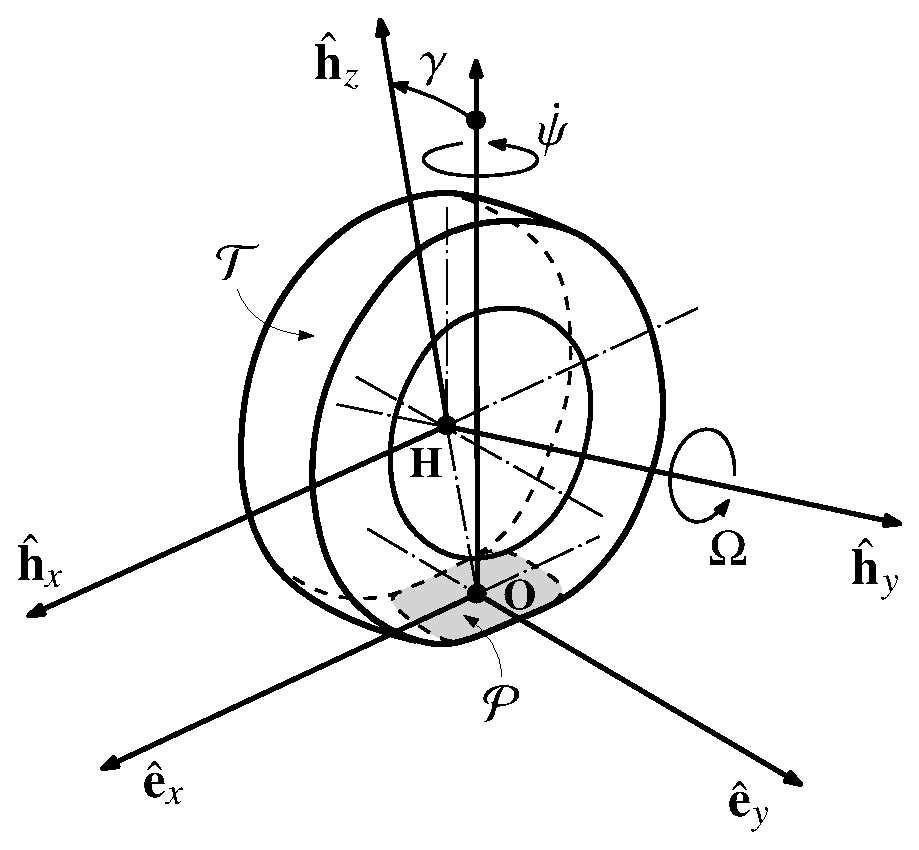
\includegraphics[width=0.9\linewidth]{figures/appendix_3/tire_iso}
    \caption{Tire-road schematics according to ISO coordinate system~\cite{iso88552011}.}
    \label{app3:fig:tire_iso}
  \end{minipage}
  \hfill
  \begin{minipage}[t]{0.525\linewidth}
    \centering
    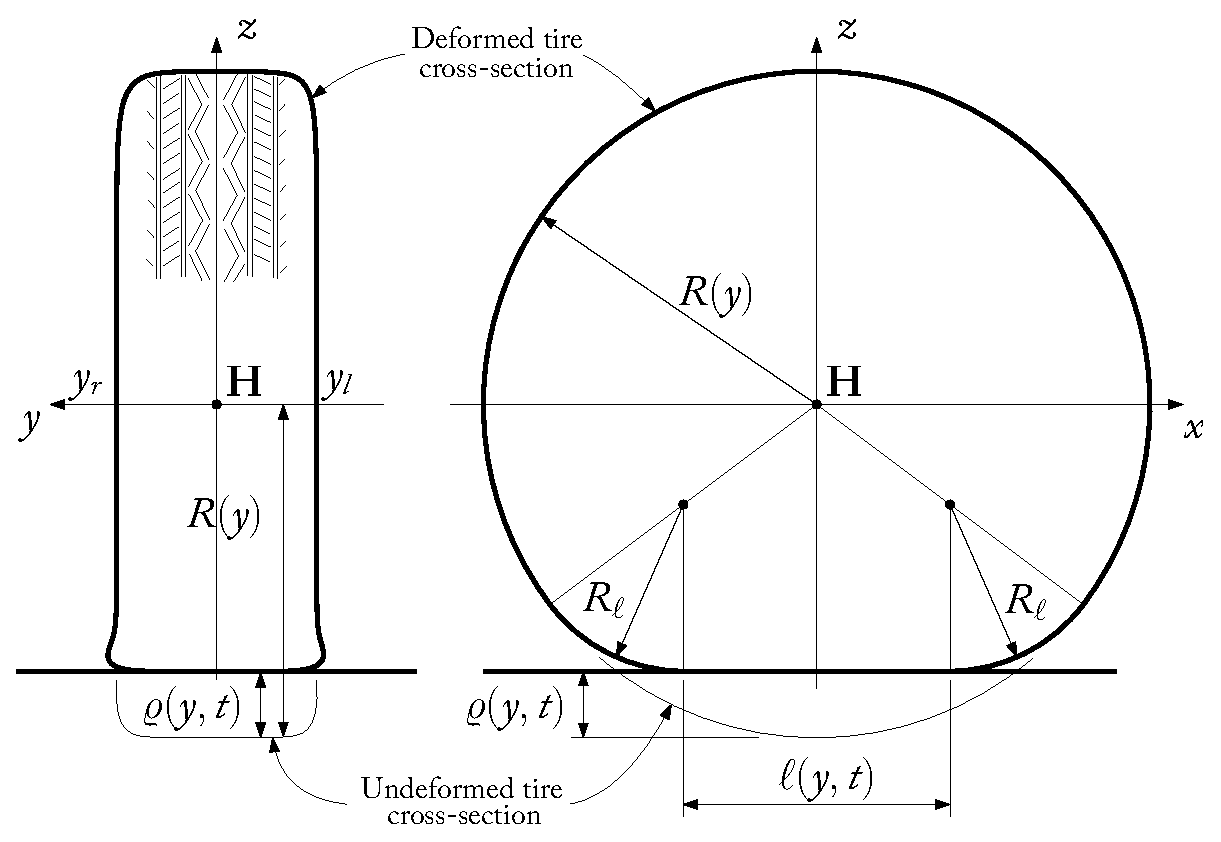
\includegraphics[width=1.0\linewidth]{figures/appendix_3/belt_section}
    \caption{Illustration of the tire-road contact geometry parameters.}
    \label{app3:fig:belt_section}
  \end{minipage}
\end{figure}

% % % % % % % % % % % % % % % % % % % % % % % % % % % % % % % % % % % % % % % %

\subsection{Tire-Road Vertical Contact Mechanics}
\label{app3:sec:vertical_contact}

When the contact patch set is not empty (\ie{}, $\sett{P} \neq \varnothing$) there is a multitude of contact points $\undx{} = [x,y,z]^\top \in \sett{P}$. At each point, the stress component along the $z$-axis (also known as normal stress) $q_z(\undx{},t)$ is applied. The integral of the normal stress distribution over the entire contact patch region is equal to the tire's vertical load $F_z(t)$. The vertical normal stress distribution is extremely difficult to calculate analytically, and it depends on the tread pattern properties, carcass stiffness, friction and inflation pressure~\cite{nakajima2019advanced}. To easily model the tire's vertical characteristics, we employ a single-contact point approach. The total vertical tire stiffness is calculated as
%
\begin{equation}
  k_z(\omega, \gamma, p) = k_z^s + k_z^p p + k_z^\omega \omega + k_z^\gamma \gamma^2 \, \text{.}
\end{equation}
%
Here, $k_z^s$ represents the structural vertical stiffness, $k_z^p$ denotes the vertical stiffness dependence on inflation pressure, $k_z^\omega$ indicates the vertical stiffness dependence on rolling speed, and $k_z^\gamma$ is the vertical stiffness dependence on camber angle. The total vertical force is thereby calculated as
%
\begin{equation}
  F_z(t) = k_z(\omega(t), \gamma(t), p) \rho(t) + c_z \dot{\rho}(t) + k_z^b \max(0, \rho(t)-\rho_b) \, \text{,}
  \label{app3:eq:vertical_force}
\end{equation}
%
where $F_z \in \mathbb{R}_{\geq 0}$, $\rho(t) \in \mathbb{R}_{\geq 0}$ represents the deflection at the tire contact point, $\rho_b$ represents the bottoming threshold, $c_z$ is the vertical damping coefficient, and $k_z^b$ indicates the bottoming vertical stiffness. Specifically, the tire contact point deflection $\rho(t)$ is calculated with the method outlined in~\cite{stocco2024novel, stocco2021acme}. This technique not only facilitates efficient and robust computation of the contact point deflection $\rho(t)$ but also allows us to compute the tire deflection $\varrho(y,t)$ at a specific lateral coordinate $y$ and time $t$. Alternatively, for cases where the technique outlined in~\cite{stocco2024novel} is not employed, a viable approximation, particularly for small camber angles ($|\gamma(t)| < \pi/10$), is
%
\begin{equation}
  \rho(t) = \max_{y \, \in \, [y_l, y_r]} \varrho(y,t) \qquad \text{(refer to \figurename~\ref{app3:fig:belt_section})} \, \text{.}
\end{equation}

\subsubsection{Contact Patch Length}
\label{app3:sec:contact_patch}

The geometrical intersection between the tire set $\sett{T}$ and road boundary surface $\boundary{R}$ provides us only a rough approximation of the tire-road contact patch area. Based on the findings in~\cite{koutny2007geometry, rhyne2005development}, we introduce a contact transition radius $R_\ell \in \mathbb{R}_{\geq 0}$ to take the tire belt stiffness into account and get a more realistic result (see \figurename~\ref{app3:fig:belt_section}). The contact length at any given lateral coordinate $y$ on the contact patch reference system can be computed as
%
\begin{equation}
  \ell(y,t) = 2\sqrt{\big(2(R(y)-R_\ell) - \varrho(y,t)\big)\varrho(y,t)} \, \text{,}
  \label{app3:eq:contact_length}
\end{equation}
%
where $\varrho(y,t)$ is the tire radial deflection. Notice that the equation~\eqref{app3:eq:contact_length} can be easily found from the study of \citet{rhyne2005development} by imposing null radial counter-deflection.

\subsubsection{Contact Pressure Distribution}
\label{app3:sec:pressure_distribution}

The pressure distribution is one of the most complex, challenging-to-model factors significantly impacting tire behavior~\cite{savkoor1966some}. Both experimental results and \ac{FE} analyses reveal that the pressure trend over the contact patch is strongly three-dimensional and is influenced by numerous factors, including carcass structural stiffness, contact pressure, relative camber angle, tread pattern topology, and local road macro-roughness. Experimental evidence suggests that adequately inflated modern radial tires typically exhibit a plateau in the pressure distribution at the central part of the contact patch~\cite[Chapter~5]{nakajima2019advanced}. Conversely, overinflated and underinflated radial tires may have more complicated distribution shapes~\cite{nakajima2019advanced, sakai1995measurement}. Recent efforts have been aimed at more detailed modeling of the contact patch to better match experimental results~\cite{miyashita2010tire, fevrier2013method, xu2014analytical}. An interesting approach involves modeling the contact pressure distribution using a quartic polynomial function $\Upsilon(\chi) = c_0 + c_1\chi^1 + c_2\chi^2 + c_3\chi^3 + c_4\chi^4$. This function represents the normalized contact pressure distribution shape along the normalized longitudinal coordinate $\chi \in [0, 1]$. To determinate the polynomial coefficients $c_0, \dots, c_4$ the following constraints are imposed
%
\begin{equation}
  \begin{cases}
    \dfrac{\mathrm{d}^2}{\mathrm{d}\chi^2}\Upsilon\left(\dfrac{1}{2}\right) = -\lambda & \text{convexity at the center of the contact patch $\chi = \dfrac{1}{2}$,}
    \\[1em]
    \displaystyle\int_{0}^{1} \Upsilon(\chi)\,\mathrm{d}\chi = 1 & \text{normalization condition for the total contact force over the contact patch,}
    \\[1em]
    \displaystyle\int_{0}^{1} \Upsilon(\chi)\chi\,\mathrm{d}\chi = \dfrac{1}{2} - \delta & \text{barycentre shift with respect to the center of the contact patch $\chi = \dfrac{1}{2}$,}
    \\[1.5em]
    \Upsilon(0) = \Upsilon(-1) = 0 & \text{absence of pressure at the edges of the contact patch $\chi = 0$ and $\chi = 1$.}
    \\[0.5em]
  \end{cases}
  \label{app3:eq:upsilon}
\end{equation}
%
Then, we solve for $c_0, \dots, c_4$, and the solution of the system is
%
\begin{equation*}
  c_0 = 0, \quad
  c_1 = -\dfrac{1}{3}\lambda + 10 + 60\delta, \quad
  c_2 = 2\lambda - 30 - 180\delta, \quad
  c_3 = -\dfrac{10}{3}\lambda + 40 + 120\delta, \quad \text{and} \quad
  c_4 = \dfrac{5}{3}\lambda - 20.
\end{equation*}
%
Here, $\lambda \in \mathbb{R}$ and $\delta \in \mathbb{R}$ respectively denote the convexity and longitudinal barycentre shift of the base curve $\Upsilon(\chi)$. The only drawback of this approach is that for certain values of $\delta$ and $\lambda$, the condition of positive pressure $\Upsilon(\chi) \ge 0$ within the range $\chi \in [0,1]$ is not always guaranteed and must be numerically checked in the software implementation. Thus, a careful selection of these parameters is essential. On the other hand, the use of a polynomial to describe the pressure distribution over the contact patch allows us to adopt some numerically robust algorithms and efficient evaluations for some of the calculations that will follow. Given the objective of achieving real-time applicability for the numerical tire model, this aspect should not be overlooked. The vertical contact stress distribution $q_z(\undx{},t)$ is then written as
%
\begin{equation}
  q_z(\undx{},t) = \dfrac{F_z(t)}{A_\sett{P}(t)}\Upsilon\left(\dfrac{\ell(y,t)/2-x}{\ell(y,t)}\right) \, \text{,} \\
  \label{app3:eq:vertical_stress}
\end{equation}
%
where $\undx{} = [x,y,z]^\top \in \sett{P}$, $F_z$ denotes the tire's vertical load, and $A_\sett{P}$ represents the contact patch area, defined as
%
\begin{equation}
  A_\sett{P}(t) = \displaystyle\int_{y_r}^{y_l} \ell(y,t)\,\mathrm{d}y \, \text{.}
\end{equation}
%
It must be stressed that the contact patch region $\sett{P}$ is a function of time $t$ and of the lateral coordinate $y$. This variability arises because the contact patch is not fixed but rather a function of the tire-road contact geometry.

% % % % % % % % % % % % % % % % % % % % % % % % % % % % % % % % % % % % % % % %

\subsection{Tire-road Tangential Contact Mechanics}
\label{app3:sec:tangential_contact}

In the present work, we assume that the vertical problem can be decoupled from the tangential, implying that the tangential stresses do not affect the vertical one, but not vice versa. Additionally, the vertical and lateral carcass flexibility characteristics are assumed to be fully independent. In simpler terms, we assume that neither friction-related phenomena nor carcass deformation affect the vertical pressure distribution $q_z$. Consequently, we can analyze tire-road tangential contact mechanics sequentially from the vertical component, while still maintaining the tangential contact forces proportionality to the vertical load $F_z$. It is worth noting that this assumption greatly simplifies the numerical solution of the tire model, as it avoids the need to find the vertical and tangential forces through a system of nonlinear equations, which would be computationally expensive.

% % % % % % % % % % % % % % % % % % % % % % % % % % % % % % % % % % % % % % % %

\subsubsection{Carcass Deformation Model}
\label{app3:sec:carcass_model}

In numerous tire models, the carcass is modeled as a beam on elastic foundation~\cite{dehoogh2005implementing, sarkisov2019physical, gil2020inplane, nakajima2019advanced}. Experimental findings from the studies~\cite{sarkisov2019physical, gil2020inplane} demonstrate that carcass deflection comprises both bending and shears components. The significance of the shear contribution varies depending on the carcass ply cord angles. Consequently, formulations like the Timoshenko-Ehrenfest or Euler-Bernoulli beam are particularly suited to describe the lateral bending of carcass structure in the cornering conditions~\cite{gil2020inplane}. Models like those in~\cite{fiala1954seitenkraften, miyashita2006new, kabe2006new, xu2014analytical, gil2020inplane, sakai1981theoreticalI, sakai1981theoreticalII, sakai1981theoreticalIII, sakai1982theoreticalIV, miyashita2010tire, fevrier2013method} adopt a second-order polynomial (parabola) as a local approximation of the beam on elastic foundation in the proximity of contact patch area. This approach provides a straightforward yet accurate description of the deformed carcass centreline within the contact region. However, the models currently present in the literature are only able to fully describe the lateral deformation and do not allow for modeling the longitudinal displacement. Indeed, during traction, braking and cornering, the contact patch is subject to non-negligible fore-aft, lateral, bending and torsional displacements. These displacements strongly impact the generation of longitudinal, lateral, and vertical forces, as well as rolling resistance, overturning, and self-alignment torques. To take into account the longitudinal displacement of the carcass, we define the two-dimensional carcass centreline as
%
\begin{equation}
  \sett{L}(\undx{}, \vt{c}) =
  \begin{bmatrix}
    \sett{L}_x \\[0.2em]
    \sett{L}_y
  \end{bmatrix} =
  \begin{bmatrix}
    x_c \\[0.2em]
    y_c + \theta_c(x-x_c) - y_c\dfrac{\Psi}{2}(x-x_c)^2
  \end{bmatrix} \, \text{,}
  \label{app3:eq:parabola}
\end{equation}
%
where time-dependent parameters $x_c$ and $y_c$ represent the carcass longitudinal and the lateral translating deformations, respectively, $\theta_c$ denotes the carcass twisting angle, and $\Psi$ is the lateral bending shape factor. As depicted in \figurename~\ref{app3:fig:contact_patch}, we model the carcass deformation through a point $\vt{c} = [x_c, y_c, \theta_c]^\top$ described within the contact patch reference frame $\pt{O}xyz$. The carcass point $\pt{c}$ is connected through a set of independent spring elements to the point $\left[0, 0, -R_z\right]^\top$, defined in the hub reference frame $\pt{H}xyz$, where $R_z = \et{n} \cdot (\pt{H}-\pt{O})$.

\begin{figure}[htb]
  \centering
  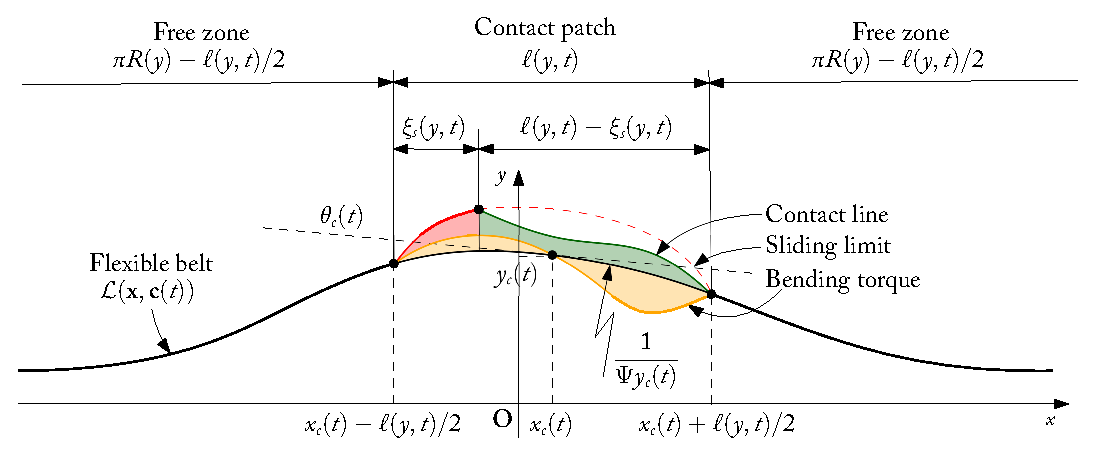
\includegraphics[width=0.8\linewidth]{figures/appendix_3/contact_patch}
  \caption{Depictions of the deformed carcass baseline $\sett{L}(\undx{}, \vt{c})$, along with the contact line of bristles, adherence limit, distribution of bending torque, and the adherence and sliding regions.}
  \label{app3:fig:contact_patch}
\end{figure}

As mentioned at the beginning of this, the carcass is the subcomponent of a tire that connects the rim to the tread and, it has a significant impact on the tire's overall behavior. From a pure physics perspective, the carcass is a system that is rigidly connected to the rim and has to deform in order to accommodate the tread's deformation. This involves balancing forces generated by the carcass state against the stresses of the tread state deformation. Thence, the carcass equilibrium equations in matrix form are written as
%
\begin{equation}
  \vt{G}(\vt{c}) = \pt{K}(\vt{c}) \vt{c} - \vt{F}(\vt{c},t) = 0 \, \text{,}
  \label{app3:eq:nls}
\end{equation}
%
where
%
\begin{equation}
  \vt{F}(\vt{c},t) =
  \begin{bmatrix}
    F_{ax}(\vt{c},t) \\[0.2em]
    F_{ay}(\vt{c},t) \\[0.2em]
    M_{az}(\vt{c},t)
  \end{bmatrix} + \begin{bmatrix}
    F_{sx}(\vt{c},t) \\[0.2em]
    F_{sy}(\vt{c},t) \\[0.2em]
    M_{sz}(\vt{c},t)
  \end{bmatrix} \, \text{,}
\end{equation}
%
and the matrix $\pt{K}$ represents the carcass stiffness matrix, which is assumed to be a diagonal matrix of the form
%
\begin{equation}
  \pt{K}(\vt{c}) =
  \begin{bmatrix}
    K_x(p,x_c) & 0 & 0 \\
    0 & K_y(p,y_c) & 0 \\
    0 & 0 & K_\theta(p,\theta_c)
  \end{bmatrix} \, \text{.}
\end{equation}
%
The entries $K_x(p,x_c)$, $K_y(p,t_c)$, and $K_\theta(p,\theta_c)$ are the longitudinal, lateral and twisting carcass stiffnesses, respectively. These values are influenced by the tire construction technology and inflation pressure $p$, as well as the deformation of the tire carcass. They can be expressed as follows
%
\begin{equation}
  \begin{split}
    \begin{aligned}
      K_x(p,x_c)           &= k_x^s      + p \, k_x^p      + k_x^b \, h(x_c, x_b, h_x) \, \text{,} \\
      K_y(p,y_c)           &= k_y^s      + p \, k_y^p      + k_y^b \, h(y_c, y_b, h_y) \, \text{,} \\
      K_\theta(p,\theta_c) &= k_\theta^s + p \, k_\theta^p + k_\theta^b \, h(\theta_c, \theta_b, h_\theta) \, \text{.} \\
    \end{aligned}
  \end{split}
\end{equation}
%
Here, the function $h(x,b,h)$ is defined as
%
\begin{equation}
  h(x,b,h) = \left(\mathrm{pos}(-x-b, h) + \mathrm{pos}(x-b, h)\right)^2 \, \text{,}
\end{equation}
%
where
%
\begin{equation}
  \mathrm{pos}(x,h) =
  \begin{cases}
    \dfrac{\sqrt{x^2 + h^2}}{2}+x    & x > 0 \\[0.5em]
    \dfrac{h^2}{2(\sqrt{x^2+h^2}-x)} & \mathrm{otherwise}
  \end{cases}
\end{equation}
%
is a regularized function of the positive part. Notice that the deformation of the tire carcass has a physical limit given by the maximum deformation of the sidewalls. For this reason, the parameters $k_x^b$, $k_y^b$, and $k_\theta^b$ are introduced to model the longitudinal, lateral and twisting bottoming stiffnesses, respectively.

\begin{figure}[htb]
  \centering
  \begin{minipage}[t]{0.475\linewidth}
    \centering
    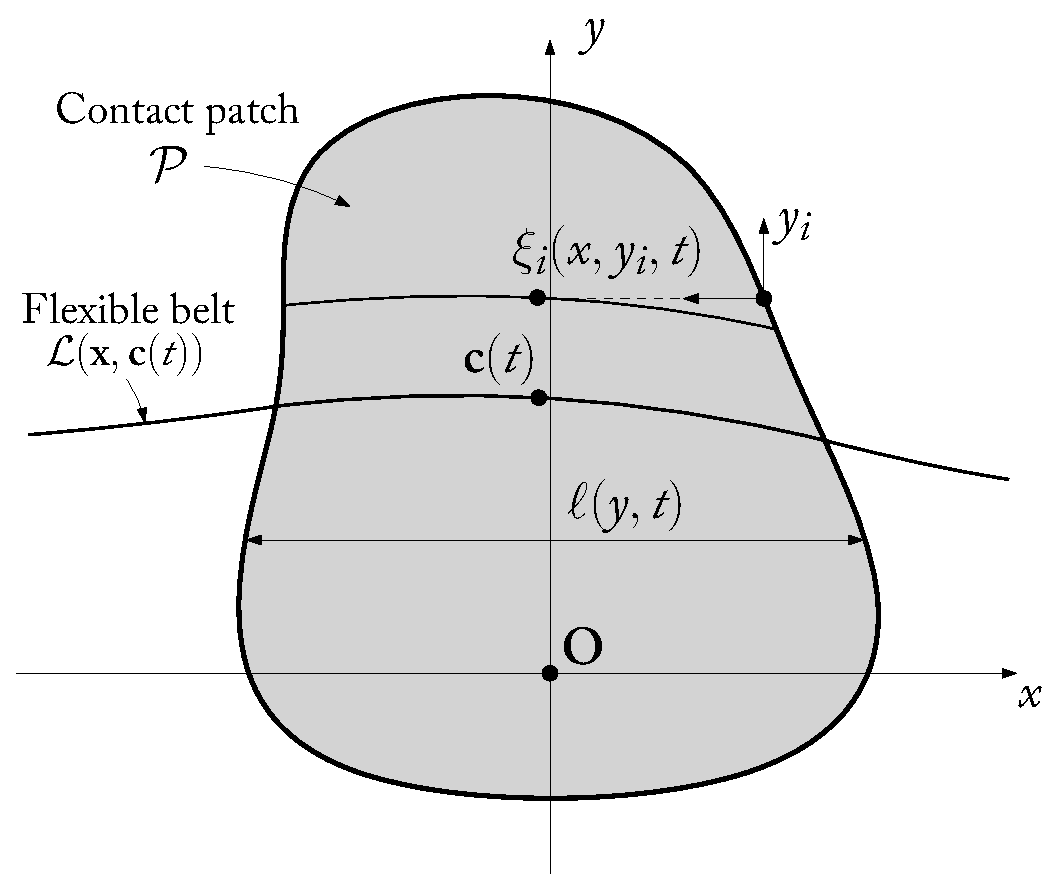
\includegraphics[width=0.9\linewidth]{figures/appendix_3/contact_patch_vertical}
    \caption{Representation of the contact patch region $\sett{P}$ and contact patch reference frame $\bm{\xi}_i(y_i,t)$. Notice that the contact patch is defined as a D-convex and arbitrary region, whose shape is described along the $y$-axis by the quantity $\ell(y,t)$.}
    \label{app3:fig:contact_patch_vertical}
  \end{minipage}
  \hfill
  \begin{minipage}[t]{0.475\linewidth}
    \centering
    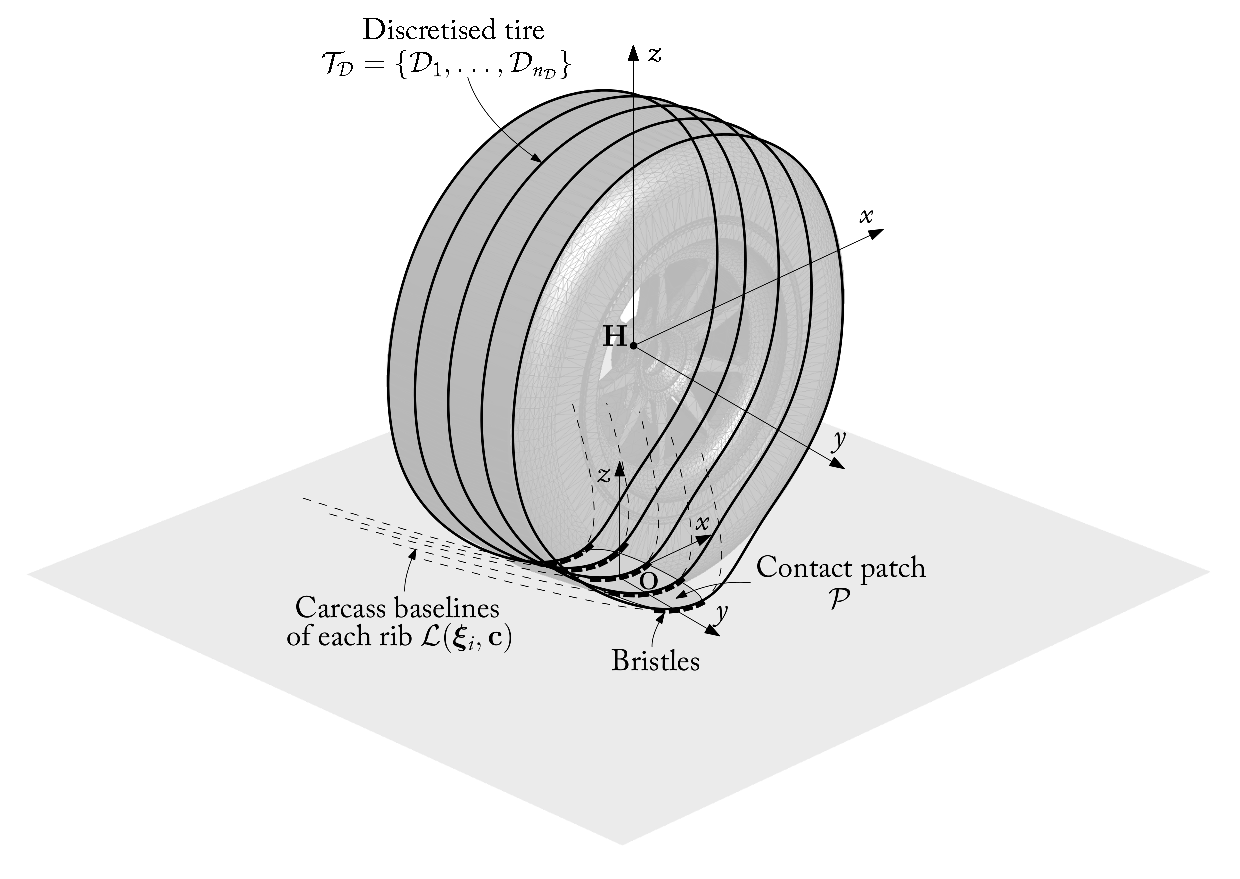
\includegraphics[width=0.9\linewidth, trim={4.35cm 3cm 4.35cm 0cm}, clip]{figures/appendix_3/brush_model}
    \caption{Illustration of the brush model. The tire $\sett{T}$ is discretized into a series of $n_\sett{D}$ ribs. Carcass and bristles are represented as the main components of the model. Conversely, the rim is assumed to be a rigid body and thus has no impact on the tire-road contact.}
    \label{app3:fig:brush_model}
  \end{minipage}
\end{figure}

\subsubsection{Tire-Road Tangential Contact Mechanics Equations}

For each point $\undx{} \in \sett{P}$, given a carcass pose $\vt{c}$, we associate a speed field $\pt{v}(\undx{}, t)$ and a displacement vector $\vt{u}(\undx{}, \vt{c}, t)$. The speed field $\pt{v}$ represents the relative speed between the outer tread layer and the road, while the displacement vector $\vt{u}$ represents the deformation of the material point (also referred to as a \emph{bristle}) located at the coordinate $\undx{}$. Additionally, each material point is also subjected to an external force $\vt{q}(\undx{}, \vt{c}, t)$ generated by the tire-road contact.

We define the generic tangential position as $\undt{}
 = x\et{e}_x + y\et{e}_y$, the tangential velocity field as $\vt{v}_{\undt{}
}(\undx{}, \vt{c}, t) = v_x(\undx{}, \vt{c}, t)\et{e}_x + v_y(\undx{},\vt{c},t)\et{e}_y$, the tangential displacement vectors as $\vt{u}_{\undt{}
}(\undx{},\vt{c},t) = u_x(\undx{},\vt{c},t)\et{e}_x + u_y(\undx{},\vt{c},t)\et{e}_y$, and the tangential stress vector as $vt{q}_{\undt{}
}(\undx{},\vt{c},t) = q_x(\undx{},\vt{c},t)\et{e}_x + q_y(\undx{},\vt{c},t)\et{e}_y$, in a such a way that
%
\begin{equation}
  \vt{v} =
  \begin{bmatrix}
    \vt{v}_{\undt{}
} \\
    v_z
  \end{bmatrix}, \qquad
  \vt{u} =
  \begin{bmatrix}
    \vt{u}_{\undt{}
} \\
    u_z
  \end{bmatrix}, \qquad \text{and} \qquad
  \vt{q} =
  \begin{bmatrix}
    \vt{q}_{\undt{}
} \\
    q_z
  \end{bmatrix} \, \text{.}
  \label{app3:eq:ut}
\end{equation}
%
The bristles tangential \emph{micro-sliding speed} is defined as
%
\begin{equation}
  \vt{v}_s(\undx{},\vt{c},t) =
  \begin{bmatrix}
    v_{sx}(\undx{},\vt{c},t) \\
    v_{sy}(\undx{},\vt{c},t)
  \end{bmatrix} \, \text{,}
\end{equation}
%
which represents the relative speed between a material point within the contact patch $\sett{P}$ and the road surface $\boundary{R}$. In the following, we will employ an isotropic steady-state Coulomb friction model, which enables us to write the equations governing the contact mechanics between the tire tread layer and the road surface as
%
\begin{equation}
  \vt{v}_s = 0 \iff \|\pt{q}_{\undt{}
}\| \leq \mu_s q_z
  \qquad \text{and} \qquad
  \vt{q}_{\undt{}
} = -\mu_d q_z \dfrac{\vt{v}_s}{\|\vt{v}_s\|}
  \iff \vt{v}_s \neq 0 \, \text{.}
  \label{app3:eq:fundamental_eqns}
\end{equation}
%
In these equations, $\mu_s$ represents the static friction coefficient and $\mu_d(\undx{}, \vt{c}, t)$ denotes the ``dynamic'' friction coefficient. It is important to note that~\eqref{app3:eq:fundamental_eqns} is only valid under the assumption of memory-less friction, meaning there is a one-to-one map between the tangential stress and the micro-sliding speed~\cite{canudasdewit2003dynamic}. To solve~\eqref{app3:eq:fundamental_eqns}, two additional sets of equations are necessary. The first set consists of the so-called \emph{tire-road kinematic equations}, which link the wheel hub's relative motion to the deformation field over the contact patch area. The second set includes the \emph{constitutive relations}, which correlate the bristles deformation field to the generated tangential stress $\vt{q}_{\undt{}
}$.

% % % % % % % % % % % % % % % % % % % % % % % % % % % % % % % % % % % % % % % %

\subsubsection{Rubber Friction}
\label{app3:sec:rubber_friction}

Friction significantly affects tire behavior. As noted in prior works~\cite{selig2014rubber, savkoor1965friction, savkoor1987dry, tiwari2017rubber}, it is influenced by various factors such as tread rubber compound, road surface roughness at both micro and macro levels, relative speed of sliding surfaces, and temperature conditions. To keep the complexity under an acceptable level, we adopt a steady-state Coulomb friction model. In doing so, the dynamic characteristic of friction,  known as \emph{frictional memory}, is disregarded. Such a behavior arises from the fact that the friction coefficient depends not only on the relative sliding speed but also on the contact history, \ie{}, the sliding trajectory~\cite{persson2010rubber}. Including this phenomenon would significantly increase the complexity of the whole tire model, necessitating a dense discretization of the tire tread layer.

Numerous physical formulations aim to capture the relationship between the friction coefficient and sliding speed. One of the most important is the \emph{Savkoor friction law}, which includes the so-called \emph{Stribeck effect}~\cite{savkoor1965friction, savkoor1966some, savkoor1987dry}. When accounting for contact pressure dependency, the ``dynamic'' friction coefficient $\mu_d(\undx{})$ can be expressed as
%
\begin{equation}
  \mu_d = \mu_w (\mu_{p_0} + \mu_{p_1} \exp( -\mu_{p_2} q_z )) (\mu_k + (\mu_s - \mu_k)) \exp\left( -\mu_{v_0}^2 \log^2 \left( \dfrac{\|\vt{v}_s\|}{v_\mu} + \mu_{v_1} \exp\left(-\dfrac{\|\vt{v}_s\|}{v_\mu}\right)\right)\right) \, \text{,}
\end{equation}
%
where
%
\begin{itemize}
  \setlength{\itemsep}{0pt}
  \item $\mu_w$ represents the friction coefficient scaling factor, used to tune the friction coefficient under different conditions, such as wet, dry, icy, etc.;
  \item $\mu_s$ is the static friction coefficient;
  \item $\mu_k$ is the kinetic friction coefficient;
  \item $\mu_{p_0}$, $\mu_{p_1}$, $\mu_{p_2}$ are parameters aimed at fitting the rubber-asphalt contact friction pressure dependency;
  \item $\mu_{v_0}$ and $\mu_{v_1}$ are parameters used to reproduce the rubber-asphalt contact friction velocity dependency;
  \item $v_\mu$ is the Stribeck velocity.
\end{itemize}

% % % % % % % % % % % % % % % % % % % % % % % % % % % % % % % % % % % % % % % %

\subsubsection{Tire-Road Kinematic Equations}
\label{app3:sec:kinematic_equations}

The relative velocity between the bristles and the road, first introduced with the name of micro-sliding velocity $\vt{v}_s$, are expressed in Eulerian form similar to that in~\cite{romano2019novel, romano2020unsteadystate, romano2022brush, romano2022analytical, pacejka2012tire, guiggiani2014science, limebeer2018dynamics}. Hence, using~\eqref{app3:eq:parabola} and~\eqref{app3:eq:ut}, $\vt{v}_s$ can be written as
%
\begin{equation}
  \vt{v}_s = V_r\left(\bm{\sigma} + \varphi\et{e}_z \times \left(\sett{L} + \undt{}
\right) + \dfrac{\mathrm{d}}{\mathrm{d}x}\sett{L}\,\right) + \dfrac{\mathrm{d}}{\mathrm{d}t}\vt{u}_{\undt{}
}
  \label{app3:eq:v_s} \, \text{,}
\end{equation}
%
where the material point deformation $\vt{u}_{\undt{}
}$ is assumed to be small. For a comprehensive description and derivation of such sliding refer to~\cite{rill2020road, pacejka2012tire, guiggiani2014science, limebeer2018dynamics, romano2019novel, romano2022brush, romano2022analytical}. The \emph{theoretical translational slips} $\bm{\sigma}$ represent the normalized difference between the longitudinal and lateral components of the speed of the wheel hub and that of the tire periphery $V_r(y,t) = \omega(t)R_r(y,t)$. Therefore, they are defined as
%
\begin{equation}
  \bm{\sigma}(y,t) =
  \begin{bmatrix}
    \sigma_x(y,t) \\[0.2em]
    \sigma_y(y,t)
  \end{bmatrix}
  = -\dfrac{1}{|V_r(y,t)|}
  \begin{bmatrix}
    V_x(t) - V_r(y,t) + \dot{x}_c(t) \\[0.2em]
    V_y(t) - R_z(t)\dot{\gamma}(t) + \dot{y}_c(t)
  \end{bmatrix} \, \text{,}
\end{equation}
%
where $\sigma_x$ and $\sigma_y$ are referred to as the \emph{longitudinal} and the \emph{lateral theoretical slips}. The \emph{theoretical spin slip} $\varphi$ is obtained from
%
\begin{equation}
  \varphi(y,t) = -\dfrac{\dot{\psi}(t) + \omega(t)\sin(\gamma(t)) + \dot{\theta}_c(t)}{|V_r(y,t)|} \, \text{.}
\end{equation}
%
The quantity $R_r$ represents the so-called \emph{real rolling radius}, which is calculated as
%
\begin{equation}
  R_r(y,t) = R(y) - \dfrac{\varrho(y,t)}{3} \, \text{.}
\end{equation}
%
Other definitions of slips are available in the literature, such as the \emph{practical longitudinal slip} $\kappa$ and \emph{slip angle} $\alpha$~\cite{pacejka2012tire}, which are defined as
%
\begin{equation}
  \begin{bmatrix}
    \kappa(y,t) \\[0.2em]
    \alpha(y,t)
  \end{bmatrix}
  =
  -\dfrac{1}{|V_x(t)|}
  \begin{bmatrix}
    V_x(t) - V_r(y,t) + \dot{x}_c(t) \\[0.2em]
    \arctan{V_y(t) - R_z(t)\dot{\gamma}(t) + \dot{y}_c(t)}
  \end{bmatrix} \, \text{,}
\end{equation}
%
and thus
%
\begin{equation}
  \begin{bmatrix}
    \sigma_x \\[0.2em]
    \sigma_y
  \end{bmatrix}
  =
  \dfrac{1}{1 + |\kappa|}
  \begin{bmatrix}
    \kappa \\[0.2em]
    -\tan(\alpha)
  \end{bmatrix} \, \text{.}
\end{equation}

Since we are using the same Eulerian form of~\cite{romano2022analytical}, the total time derivative is given by
%
\begin{equation}
  \dfrac{\mathrm{d}}{\mathrm{d}t} =  \dfrac{\partial}{\partial t} + \vt{v}_{\undt{}
} \cdot\nabla_{\undt{}
} \, \text{,}
\end{equation}
%
where $\nabla_{\undt{}
}$ collects the tangential components of the gradient, and $\partial/\partial t = 0$ since we are neglecting the viscous component of the Kelvin-Voigt element representing the rubber material point~\cite{meyers2008mechanical}. Neglecting the viscous effect of the tread rubber material eliminates any explicit time dependence in the formulation of brush model forces and torques. Consequently, the tread rubber always operates under stationary conditions. Considering these points, the total derivative of the material point can be explicitly expressed as
%
\begin{equation}
  \dfrac{\mathrm{d}}{\mathrm{d}t}\vt{u}_{\undt{}
} = \underbrace{\dfrac{\partial}{\partial t}\vt{u}_{\undt{}
}}_{=0} + \vt{v}_{\undt{}
}\cdot\nabla_{\undt{}
}\vt{u}_{\undt{}
} \, \text{,}
\end{equation}
%
where the tangential gradient is given by $\nabla_{\undt{}
} = [\partial/\partial x, \partial/\partial y]^\top$. The velocity field $\vt{v}_{\undt{}
}$ of the tread rubber is formulated as
%
\begin{equation}
  \vt{v}_{\undt{}
} = -V_r \dfrac{\dfrac{\mathrm{d}}{\mathrm{d}x} \sett{L}}{\Big\|\dfrac{\mathrm{d}}{\mathrm{d}x} \sett{L}\,\Big\|} \, \text{.}
\end{equation}
%
Given the assumption of small carcass deformations (approximatively $|x_c| < \rho_b$, $|y_c| < \rho_b$, and $|\theta_c| < \pi/10$) and small tire camber angles ($|\gamma(t)| < \pi/10$) the following relationships holds~\cite{romano2022advanced}
%
\begin{equation}
  \dfrac{\mathrm{d}}{\mathrm{d}x} \sett{L}_x \approx 1 \qquad \text{and} \qquad \dfrac{\mathrm{d}}{\mathrm{d}x} \sett{L}_y \approx 0 \, \text{.}
  \label{app3:eq:approx}
\end{equation}
%
The trajectories of the bristles moving within the contact patch are straightened in the longitudinal direction. Therefore, the formulation is constrained to a velocity field of the form $\vt{v}_{\undt{}
} = [-V_r, 0]^\top$

By separating the longitudinal and tangential displacements of the bristles, we derive the bristle micro-sliding speed formulated as
%
\begin{equation}
  \vt{v}_s = V_r\left( \vt{\bm{\sigma}} + \varphi\huvec_z \times \left(\sett{L} + \undt{}
\right) + \dfrac{\mathrm{d}}{\mathrm{d}x}\sett{L} - \dfrac{\mathrm{d}}{\mathrm{d}x}\vt{u}_{\undt{}
} \right) \, \text{.}
  \label{app3:eq:v_s_int}
\end{equation}

% - - - - - - - - - - - - - - - - - - - - - - - - - - - - - - - - - - - - - - -

\subsubsection{Constitutive Relations}
\label{app3:sec:constitutive_relations}

In the present work, we assume that -- from a frictional perspective -- two regions are identified along the contact patch region \cp{}. The first is the adhesion region \adh{}, where bristle tips do not slide with respect to the ground, generating the so-called adhesive forces. The second is the sliding region \sli{}, where bristles tips slide on the ground surface, producing instead the sliding forces. The boundary separating these two regions is called transition line $\xi_s(\bm{\xi},\vt{c},t)$. Although this assumption may be not realistic in the case of high spin slip value, it greatly simplifies the problem~\cite{romano2022advanced}. By adopting this approach, the domain corresponds to the contact patch interior \interior{P}, where the partial differential equations ruling the tire-road kinematics are defined, and the corresponding boundary conditions can be uniquely formulated on \boundary{P}~\cite{romano2022analytical}. This research aims to develop a formulation that strikes a balance between realism and computational efficiency, rather than striving for a rigorous closed-form expression for the tangential bristle contact mechanics.

\paragraph{Adhesion Region}

Each individual, material point, acting independently of others,  enters the contact patch through the leading edge in an undeformed state.  As a result of van der Waals molecular bonding and rubber indentation at the rubber/ground interface, the tip of the bristles sticks to the ground. However, due to the micro-sliding velocity $\vt{v}_s$ between the root of the bristles and the road, a tangential deflection $\vt{u}_{\undt{}
}$ starts to build up, along with tangential stress $\vt{q}_{\undt{}
}$. Initially null, this bristle deformation increases gradually along the contact length until it reaches the transition line $\xi_s(\bm{\xi},\vt{c})$. This transition line represents the contact length coordinate at which the local force exerted by the bristle deformation in adhesion equals the maximum possible static friction force.

It is important to note that within the adhesion region, the tips of the bristles do not slide relative to the ground, resulting in a zero micro-sliding velocity. Consequently, the deformation of the bristles increases along the contact length direction with a spatial derivative equal to
%
\begin{equation}
  \dfrac{\mathrm{d}}{\mathrm{d}x}\vt{u}_{\undt{}
} =
  \dfrac{\mathrm{d}}{\mathrm{d}x}
  \begin{bmatrix}
    u_x \\[0.2em]
    u_y
  \end{bmatrix} \, \text{,}
  \label{app3:eq:u_dx}
\end{equation}
%
which is easily found from~\eqref{app3:eq:v_s_int} by imposing $\vt{v}_s = 0$.

We now introduce a new contact patch coordinate system (also depicted in \figurename~\ref{app3:fig:contact_patch_vertical})
%
\begin{equation}
  \bm{\xi}(y,t) =
  \begin{bmatrix}
    \xi(x,y,t) \\[0.2em]
    \eta \\[0.2em]
    \zeta
  \end{bmatrix}
  =
  \begin{bmatrix}
    \ell(y,t)/2-x \\[0.2em]
    y \\[0.2em]
    z
  \end{bmatrix} \, \text{.}
\end{equation}
%
The variable $\xi$ represents the distance from the entrance to the longitudinal coordinate, measured longitudinally from the contact patch leading edge. From now on, we will use the superscript ``$\,\bm{\xi}\,$'' to denote variables described in reference system $\bm{\xi}$, \eg{}, $\vt{u}_{\undt{}
}(\bm{\xi},\vt{c})$. Substituting $\bm{\xi}$ in~\eqref{app3:eq:u_dx} we obtain
%
\begin{equation}
  \dfrac{\mathrm{d}}{\mathrm{d}\xi}\vt{u}_{\undt{}
}^{\bm{\xi}} =
  \dfrac{\mathrm{d}}{\mathrm{d}\xi}
  \begin{bmatrix}
    u_{x}^{\bm{\xi}} \\[0.2em]
    u_{y}^{\bm{\xi}}
  \end{bmatrix} \, \text{.}
  \label{app3:eq:u_dxi}
\end{equation}
%
The specific deformation $\vt{u}_{\undt{}
}^{\bm{\xi}}$ at a contact length coordinate $\xi$ and lateral coordinate $y$ is obtained from integrating~\eqref{app3:eq:u_dxi} over space, while imposing the boundary condition $\vt{u}_{\undt{}
}(\undx{} = [0,y,0]^\top,\vt{c}) = 0$, namely
%
\begin{equation}
  \vt{u}_{\undt{}
}^{\bm{\xi}} = \int_0^\xi \dfrac{\mathrm{d}}{\mathrm{d}\zeta}\vt{u}_{\undt{}
}(\zeta,\vt{c}) \,\mathrm{d}\zeta.
  \label{app3:eq:u_xi}
\end{equation}
%
The infinitesimal adherence force at a specific contact length coordinate $\xi$ is determined by the product between~\eqref{app3:eq:u_xi} and the tread tangential stiffness matrix $\pt{k}$
%
\begin{equation}
  \vt{q}_{\undt{}
}^{\bm{\xi}} = -\nu\pt{K}_{\undt{}
}\vt{u}_{\undt{}
}^{\bm{\xi}} \, \text{.}
  \label{app3:eq:fa}
\end{equation}
%
Here, $\nu$ represents the tread pattern void ratio, and $\pt{K}_{\undt{}
}$ denotes the tangential stiffness matrix. This latter is typically expressed as
%
\begin{equation}
  \pt{K}_{\undt{}
} =
  \begin{bmatrix}
    k_{xx} & k_{yx} \\[0.2em]
    k_{yx} & k_{yy}
  \end{bmatrix} \, \text{,}
\end{equation}
%
where $k_{xy} \approx k_{yx} \ll k_{xx} \approx k_{yy}$, as proofed by \citet{okonieski2003simpified}. The total bristles force induced by the deformation in adherence is obtained by integrating the following over the entire adhesion region \adh{}
%
\begin{equation}
  \vt{F}_a(\vt{c},t) = \int_{\adh} \vt{q}_{\undt{}
}^{\bm{\xi}} \mathrm{d}\bm{\xi} \, \text{.}
  \label{app3:eq:F_a}
\end{equation}

In the original brush model presented in~\cite{pacejka2012tire}, the self-aligning moment is attributed solely to the asymmetrical distribution of lateral shear stress along the contact length. However, in this study, we will also consider that the difference in longitudinal force on each side of the contact patch contributes to the generation of the self-aligning moment. Thereby, the adhesive self-aligning moment is defined as the cross-product between forces induced by deformation and the position vector (the sum of bristle position and carcass baseline position vectors), which reads
%
\begin{equation}
  \vt{M}_{a}(\vt{c},t) = \int_{\adh} \vt{q}_{\undt{}
}^{\bm{\xi}} \times \left(\sett{L}^{\bm{\xi}} + \bm{\xi}\right) \mathrm{d}\bm{\xi} \, \text{.}
  \label{app3:eq:M_a}
\end{equation}

\paragraph{Slide Region}

When the local force induced by bristle deformation in adhesion is greater than the local maximum explicable static friction force, the bristle tips begin to slide over the ground with a micro-sliding velocity $\vt{v}_s^{\bm{\xi}} \neq 0$. The local force exerted by bristle deformation in sliding opposes the micro-sliding velocity. Thus, its direction is denoted as
%
\begin{equation}
  \vt{d}_{\undt{}
}(\bm{\xi},\vt{c}) =
  \begin{bmatrix}
    d_{tx}(\bm{\xi},\vt{c}) \\[0.2em]
    d_{ty}(\bm{\xi},\vt{c})
  \end{bmatrix} =
  -\dfrac{\vt{v}_s^{\bm{\xi}}}{\|{\vt{v}_s^{\bm{\xi}}}\|} \, \text{.}
\end{equation}
%
The total bristles force induced by the deformation in sliding is determined by integrating the following expression over the entire sliding region \sli{}
%
\begin{equation}
  \vt{F}_s(\vt{c},t) = \int_{\sli} \mu_d^{\bm{\xi}}\,q_z^{\bm{\xi}}\,\vt{d}_{\undt{}
}^{\bm{\xi}} \, \mathrm{d}\bm{\xi} \, \text{.}
  \label{app3:eq:F_s}
\end{equation}
%
Similar to the adhesive scenario, the self-aligning moment is defined as the cross-product between the local force induced by the sliding and the position vector
%
\begin{equation}
  \vt{M}_s(\vt{c},t) = \int_{\sli} \mu_d^{\bm{\xi}}\,q_z^{\bm{\xi}}\,\vt{d}_{\undt{}
}^{\bm{\xi}} \times \left(\sett{L}^{\bm{\xi}} + \bm{\xi}\right) \mathrm{d}\bm{\xi} \, \text{.}
  \label{app3:eq:M_s}
\end{equation}

% % % % % % % % % % % % % % % % % % % % % % % % % % % % % % % % % % % % % % % %

\section{A Numerical Solution Approach}
\label{app3:sec:numerical_solution}

Due to the complexity of the problem outlined in the preceding sections, finding an analytical solution is not feasible. Therefore, we need to further analyze the contact zone between the tire and the road and set some more assumptions that will allow us to obtain an effective numerical scheme.

\subsection{Tire-Road Contact Discretization}

An essential characteristic of the contact patch set $\sett{P}$ is its constant compactness and D-convexity along the $\et{e}x$ direction~~\cite{romano2022analytical, matouvsek2001directional}. Leveraging the D-convexity properties enables us to discretize the contact patch into longitudinal sections. To optimize the intersection of the tire and road sets, we discretized the tire set $\sett{T}$ into a series of $n_\sett{D}$ ribs, similarly to the approach in~\cite{chollet2012model, stocco2024novel}. Each tire rib, denoted as $\sett{D}$, is characterized as a conical frustum which is located in $\pt{o}= [0,y_\sett{D},0]^\top$ in the $\pt{H}xyz$ coordinate system, with a radius of $R(y_\sett{D})$ and a width of $w_\sett{D}$
%
\begin{equation}
  \sett{D} = \left\{ w_\sett{D}, y_\sett{D} \in \mathbb{R}, \pt{x} = \left[ x, y, z \right]^\top \in \mathbb{R}^3 ~|~ \sqrt{x^2+z^2} \leq R(y_\sett{D}), |y-y_\sett{D}| \leq \dfrac{w_\sett{D}}{2} \right\} \, \text{.}
\end{equation}
%
This new representation allows us to build the discretized tire set $\sett{T}_\sett{D}$ as
%
\begin{equation}
  \sett{T}_\sett{D} = \left\{ \sett{D}_1, \sett{D}_2, \dots, \sett{D}_{n_\sett{D}-1}, \sett{D}_{n_\sett{D}} \right\} \, \text{.}
\end{equation}
%
Notice that we will employ a set of contact patch coordinate systems $\bm{\xi}_i$ equal to the ribs $n_\sett{D}$. These coordinate systems are redefined as
%
\begin{equation}
  \bm{\xi}_i(x, y_i, t) =
  \begin{bmatrix}
    \xi_i(x, y_i, t) \\
    \eta_i \\
    \zeta
  \end{bmatrix}
  =
  \begin{bmatrix}
    \ell(y_i, t)/2 - x \\
    y_i \\
    z_i(x)
  \end{bmatrix} \, \text{,}
\end{equation}
%
where $z_i(x)$ represents the height of the rib $i$ at the point $x$, considering the possibility of the contact patch being sloped in the longitudinal direction. Similar to our previous approach, the variables described in the reference system $\bm{\xi}_i$ will be denoted with the superscript ``$\,\bm{\xi}_{i}\,$'', \eg{}, $\vt{u}_{\pt{t}}(\bm{\xi}_{i}, \vt{c})$. It is worth noting that this tire representation is fully adjustable in scale, allowing for the density of ribs representing the tire to be tailored based on the required accuracy and computational speed for a specific simulation.

By applying the considerations and assumptions outlined in Section~\ref{app3:sec:constitutive_relations} to the constitutive relations, we can express the integrals of forces and moments relative to the adhesion and sliding zones as summations of the components from each rib. Specifically, if the transition coordinate $\xi_s^i$ is assumed to be known, the integrals~\eqref{app3:eq:F_a} and \eqref{app3:eq:M_a} can be analytically solved. Conversely, integrals~\eqref{app3:eq:F_s} and \eqref{app3:eq:M_s} must be numerically calculated.

\subsection{The Transition Coordinate}

Starting from the beginning of each rib contact region, the bristle tips stick to the ground up to the transition coordinate $\xi_s^i$. Determining $\xi_s^i$ entails locating the precise point where the local force induced by bristle deformation in adhesion equals the local maximum static friction force that can be sustained. This requires applying the adhesion criteria outlined in~\eqref{app3:eq:fundamental_eqns}
%
\begin{equation}
  \left(q_{x}^{\bm{\xi}i}\right)^{2} + \left(q_{y}^{\bm{\xi}i}\right)^{2} = \left(\mu_s q_{z}^{\bm{\xi}i}\right)^{2} \, \text{.}
  \label{app3:eq:transition}
\end{equation}

Due to the complexity of the pressure distribution model and the shear field description, finding an analytical solution to equation~\eqref{app3:eq:transition} is not feasible. However, through calculus, it can be demonstrated that the longitudinal and lateral tangential stresses $q_{x}^{\bm{\xi}i}$, $q_{y}^{\bm{\xi}i}$, and normal stress $q_{z}^{\bm{\xi}i}$ can be described by polynomial functions. Consequently, both the right- and left-hand sides of~\eqref{app3:eq:transition} are also polynomials. We can therefore exploit many powerful and robust root-finding algorithms, like Sturm's sequence and the Bisection methods~\cite{bulirsch2002introduction} or the Algorithm 748 by~\citet{alefeld1995algorithm}.

\subsection{Tire Nonlinear System and Solution Method}

As mentioned earlier, the tire significantly impacts vehicle handling behavior, with carcass compliance being crucial for both steady-state and transient tire behaviors. However, most tire models similar to the one presented in this appendix lack or miss sufficient discussion on the numerical method's performance in computing carcass deformation. This involves balancing forces generated by the carcass state against the stresses of the tread state deformation. In this section, we introduce a numerical scheme designed to address this task efficiently, comparing its performance with existing methods in the literature.

The carcass equilibrium equation in matrix form is written as
%
\begin{equation}
  \vt{G}(\vt{c}) = \pt{K}(\vt{c}) \vt{c} - \vt{F}(\vt{c},t) = 0 \, \text{,}
  \label{app3:eq:nls}
\end{equation}
%
where
%
\begin{equation}
  \vt{F}(\vt{c},t) =
  \begin{bmatrix}
    F_{ax}(\vt{c},t) \\[0.2em]
    F_{ay}(\vt{c},t) \\[0.2em]
    M_{az}(\vt{c},t)
  \end{bmatrix} + \begin{bmatrix}
    F_{sx}(\vt{c},t) \\[0.2em]
    F_{sy}(\vt{c},t) \\[0.2em]
    M_{sz}(\vt{c},t)
  \end{bmatrix} \, \text{,}
\end{equation}
%
and the matrix $\pt{K}$ represents the carcass stiffness matrix, which is assumed to be a diagonal matrix of the form
%
\begin{equation}
  \pt{K}(\vt{c}) =
  \begin{bmatrix}
    K_x(p,x_c) & 0 & 0 \\
    0 & K_y(p,y_c) & 0 \\
    0 & 0 & K_\theta(p,\theta_c)
  \end{bmatrix} \, \text{.}
\end{equation}
%
The entries $K_x(p,x_c)$, $K_y(p,t_c)$, and $K_\theta(p,\theta_c)$ are the longitudinal, lateral and twisting carcass stiffnesses, respectively. These values are influenced by the tire construction technology and inflation pressure $p$, as well as the deformation of the tire carcass. They can be expressed as follows
%
\begin{equation}
  \begin{split}
    \begin{aligned}
      K_x(p,x_c)           &= k_x^s      + p \, k_x^p      + k_x^b \, h(x_c, x_b, h_x), \\
      K_y(p,y_c)           &= k_y^s      + p \, k_y^p      + k_y^b \, h(y_c, y_b, h_y), \\
      K_\theta(p,\theta_c) &= k_\theta^s + p \, k_\theta^p + k_\theta^b \, h(\theta_c, \theta_b, h_\theta) \, \text{.} \\
    \end{aligned}
  \end{split}
\end{equation}
%
Here, the function $h(x,b,h)$ is defined as
%
\begin{equation}
  h(x,b,h) = \left(\mathrm{pos}(-x-b, h) + \mathrm{pos}(x-b, h)\right)^2 \, \text{,}
\end{equation}
%
where
%
\begin{equation}
  \mathrm{pos}(x,h) =
  \begin{cases}
    \dfrac{\sqrt{x^2 + h^2}}{2}+x    & x > 0 \\[0.5em]
    \dfrac{h^2}{2(\sqrt{x^2+h^2}-x)} & \mathrm{otherwise}
  \end{cases}
\end{equation}
%
is a regularized function of the positive part. Notice that the deformation of the tire carcass has a physical limit given by the maximum deformation of the sidewalls. For this reason, the parameters $k_x^b$, $k_y^b$, and $k_\theta^b$ are introduced to model the longitudinal, lateral and twisting bottoming stiffnesses, respectively.

To solve~\eqref{app3:eq:nls}, an efficient iterative approach satisfying real-time constraints is necessary. Many tire models, such as those in~\cite{gruber2012normalI, gruber2012normalII, miyashita2010tire, miyashita2003analytical, miyashita2006new, kabe2006new, miyashita2015study}, employ Picard's Iteration Method (also known as the Fixed-Point Method), which is simple to implement but suffers from a slow convergence rate, potentially compromising model robustness. Alternatively, \TaMeTire{} employs a mixed Newton/quasi-Newton iterative method~\cite{fevrier2013method}. If the Jacobian $\vt{J}_\pt{G}$\footnote{$\vt{J}_\pt{G}(\vt{c}) = \partial\vt{G}(\vt{c})/\partial\vt{c}$.} is unavailable, \emph{quasi-Newton} methods can be utilized, albeit with a slight decrease in convergence rate and robustness. Notice that the Frobenius norm\footnote{For a matrix $\pt{A}\in\mathbb{R}^{n \times m}$, the Frobenius norm is defined as $\|\pt{A}\|_\mathrm{F}=\sqrt{\sum_{ij}A_{ij}^2}$.} of the Jacobian $\vt{J}_\pt{F}$\footnote{$\vt{J}_\pt{F}(\vt{c}) = \partial\vt{F}(\vt{c})/\partial\vt{c}$.} is typically small ($\|\vt{J}_\pt{F}\|_\mathrm{F} \ll 1$), while the Frobenius norm of the carcass stiffness matrix Jacbobian $\vt{J}_\pt{K}$ is usually large ($\|\vt{J}_\pt{K}\|_\mathrm{F} \gg 1$). Therefore, a good first approximation of $\vt{J}_\pt{G}$ is given by
%
\begin{equation}
  \vt{J}_\pt{G} = \vt{J}_\pt{K} - \vt{J}_\pt{F} \approx \vt{J}_\pt{K} \, \text{.}
  \label{app3:eq:jacobian_approx}
\end{equation}
%
If we set the initial iteration point at $\vt{c} = [0,0,0]^\top$, the bottoming effect of the carcass stiffness is absent. As a consequence, the initial estimation of the Jacobian $\vt{J}_\pt{G}$ can be straightforwardly computed by accounting solely for the structural and inflation pressure components of the carcass stiffness.

% % % % % % % % % % % % % % % % % % % % % % % % % % % % % % % % % % % % % % % %

\section{Numerical Performance and Validation}
\label{app3:sec:numerical_experiments}

In this section, we present numerical simulations to validate the tire model and the numerical solution approach. Specifically, we will compare the performance of the quasi-Newton methods used to solve the non-linear system of equations~\eqref{app3:eq:nls}, as well as the fitting quality of the tire model to experimental data. A comparison with the \MagicFormulae{} is also provided.

\subsection{Performance of the Quasi-Newton Methods}

We evaluate the performance of the quasi-Newton numerical methods mentioned earlier. Specifically, we aim to identify the most suitable method for solving the non-linear system of equations~\eqref{app3:eq:nls} among Picard Iteration Method (PIM), Greenstadt's $1^\text{st}$ Method (G1M)~\cite{spedicato1978some}, Greenstadt's $2^\text{nd}$ Method (G2M)~\cite{spedicato1978some}, Eirola-Nevanlinna Method (ENM)~\cite{eirola1989accelerating}, Broyden's Bad Method (BBM)~\cite{broyden1965class},
Broyden's Good Method (BGM)~\cite{broyden1965class}, Broyden's Combined Method (BCM)~\cite{martinez1982sobre}, and their respective dumped versions, denoted with the prefix ``D-''. We will compare these algorithms based on function evaluations, iterations, convergence speed, and success ratio. Table~\ref{app3:tab:timing} presents the performance data of the quasi-Newton solvers. The tests are conducted on a set of $10^5$ simulations with inputs distributed evenly within the following ranges $\sigma_x\in[-1,1]$, $\sigma_y\in[-1,1]$, $\varphi\in[-0.1,0.1]$, $F_z\in[0,5\cdot10^5]$, and $\gamma \in [-\pi/10, \pi/10]$, which represent typical operating conditions for a passenger car tire. All tests are performed on a shielded CPU. The simulation platform is a Concurrent\textsuperscript{\textregistered} iHawk\textsuperscript{\texttrademark} with \SI{2.5}{\giga\hertz} Intel\textsuperscript{\textregistered} Xeon\textsuperscript{\textregistered} Silver 4215 8-core, \SI{11}{\mega\byte} cache, \SI{32}{\giga\byte} DDR4 \ac{RAM}, and \SI{64}{\bit} RedHawk\textsuperscript{\texttrademark} Linux real-time operative system with CentOS distribution.

As depicted in Table~\ref{app3:tab:timing}, both the PIM and D-PIM fail to converge to the solution with the required tolerance. The G1M and D-G1M can not complete the tests due to overflow issues. Conversely, the G2M and ENM, and their dumped version, D-G2M and D-ENM, show a good success ratio but exhibited high average and variance iterations and function evaluations. Although the pure BBM suffered from overflow issues, its dumped version, D-BBM, successfully converged to the solution with the required tolerance and maintained an acceptable success ratio. The BGM and BCM, as well as their dumped versions, D-BGM and D-BCM, demonstrated the best performance overall. They exhibited the highest success ratio and the lowest average and variance in both iterations and function evaluations. Notably, the BCM showed superior computational efficiency. It is worth mentioning that no relaxation steps were accepted in D-BCM. Consequently, the performance of the BCM method is deemed excellent for meeting the demands of hard real-time simulations, \ie{}, achieving a computational time of less than \SI{1}{\milli\second}. Only a small percentage of the tests required and a high number of iterations, however, in these cases the vertical load and resulting carcass deformations exceeded the structural limits, leading to instability in the iterative process.

The bottom part of Table~\ref{app3:tab:timing} presents the performance of the BCM in relation to the number of ribs. Notably, the number of ribs does not impact the efficacy of the iterative method but merely affects the computational time. This arises from the fact that a change in the number of ribs does not alter the number of unknowns in~\eqref{app3:eq:nls}. Consequently, the computational time scales linearly with the number of ribs. However, it is worth noting that the variance of the computational time increases more than linearly due to small yet significant variations in the performance of Algorithm 748.

\begin{table}[htb]
  \centering
  \caption{Comparison between quasi-Newton methods' performance based on a dataset comprising $10^5$ tests. The inputs are evenly distributed within the ranges $\sigma_x \in [-1, 1]$, $\sigma_y \in [-1, 1]$, $\varphi \in [-0.1, 0.1]$, $F_z \in [0, 5\cdot10^5]$, and $\gamma \in [-\pi/10, \pi/10]$, using a 325/660R13 race car tire discretized with $5$ ribs. Convergence is considered achieved when $\|\pt{G}(\vt{c})\|_2 \le 10^{-8}$ and $\|\vt{c}_{k+1} - \vt{c}_{k}\|_2 \le 10^{-16}$. Maximum algorithm iteration and relaxation steps are set to 100 and 10, respectively. The bottom part of the table demonstrates the impact of changing the number of ribs on the BCM method's performance. \\
  \emph{Symbols legend}: \mini{} minimum number of evaluations/iterations, \maxi{} maximum number of evaluations/iterations, \meai{} average evaluations/iterations, \vari{} evaluations/iterations variance.
  }
  \label{app3:tab:timing}
  \small
  {\footnotesize\begin{tabularx}{0.75\textwidth}{*{6}{Y}}%{\textwidth}{*{14}{Y}}
  %\multicolumn{14}{c}{\textbf{Quasi-Newton Methods Performance with 5 Ribs}} \\
  \multicolumn{6}{c}{\textbf{Quasi-Newton Methods Performance with 5 Ribs}} \\
  \toprule
  \multirow{2.25}{*}{\textbf{Method}} &
  %\multicolumn{4}{c}{\textbf{Evaluations} ($-$)} &
  %\multicolumn{4}{c}{\textbf{Iterations} ($-$)} &
  \multicolumn{4}{c}{\textbf{Time} (\USI{\micro\second})} &
  \multirow{2}{*}{\textbf{Success}} \\
  \cmidrule(l{4pt}r{4pt}){2-5}
  %\cmidrule(l{4pt}r{4pt}){6-9}
  %\cmidrule(l{4pt}r{4pt}){10-13}
  %& \mini{} & \maxi{} & \meai{} & \vari{} & \mini{} & \maxi{} & \meai{} & \vari{}
    & \mini{} & \maxi{} & \meai{} & \vari{} & \\
  \midrule
  PIM   %& $100$ & $100$ & $100.0$ & $0.00$    & $100$ & $100$ & $100.0$ & $0.0$
    & $518.0$ & $7949.0$ & $617.2$  & $13953.2$  & $0.0\%$   \\ \hline
  G1M   %& $-$   & $-$   & $-$     & $-$       & $-$   & $-$   & $-$     & $-$
    & $-$     & $-$      & $-$      & $-$        & Overflow  \\ \hline
  G2M   %& $4$   & $100$ & $9.2$   & $55.8$    & $4$   & $100$ & $9.2$   & $55.8$
    & $23.5$  & $1089.4$ & $69.0$   & $5252.0$   & $99.5\%$  \\ \hline
  ENM   %& $6$   & $200$ & $11.9$  & $234.0$   & $3$   & $100$ & $6.5$   & $58.5$
    & $25.0$  & $2025.0$ & $81.5$   & $11002.8$  & $99.4\%$  \\ \hline
  BBM   %& $-$   & $-$   & $-$     & $-$       & $-$   & $-$   & $-$     & $-$
    & $-$     & $-$      & $-$      & $-$        & $0.0\%$   \\ \hline
  BGM   %& $4$   & $100$ & $8.8$   & $18.4$    & $4$   & $100$ & $8.8$   & $18.4$
    & $22.6$  & $948.1$  & $62.5$   & $1973.0$   & $99.9\%$  \\ \hline
  BCM   %& $4$   & $17$  & $8.4$   & $6.7$     & $4$   & $17$  & $8.4$   & $6.7$
    & $22.9$  & $264.4$  & $55.7$   & $885.9$    & $100.0\%$ \\ \hline
  D-PIM %& $100$ & $496$ & $190.7$ & $13628.1$ & $100$ & $100$ & $100.0$ & $0.0$
    & $507.0$ & $5383.0$ & $1151.9$ & $568491$   & $0.0\%$   \\ \hline
  D-G1M %& $-$   & $-$   & $-$     & $-$       & $-$   & $-$   & $-$     & $-$
    & $-$     & $-$      & $-$      & $-$        & Overflow  \\ \hline
  D-G2M %& $4$   & $376$ & $11.3$  & $572.4$   & $4$   & $100$ & $9.3$   & $57.1$
    & $21.5$  & $3195.5$ & $80.4$   & $40321.9$  & $99.5\%$  \\ \hline
  D-ENM %& $6$   & $513$ & $12.8$  & $829.7$   & $3$   & $100$ & $6.3$   & $44.3$
    & $27.0$  & $5207.7$ & $97.5$   & $52752.6$  & $99.5\%$  \\ \hline
  D-BBM %& $4$   & $125$ & $11.0$  & $58.0$    & $4$   & $42$  & $9.3$   & $12.8$
    & $22.3$  & $1284.0$ & $76.9$   & $5126.3$   & $100.0\%$ \\ \hline
  D-BGM %& $4$   & $376$ & $9.7$   & $110.6$   & $4$   & $100$ & $8.7$   & $15.1$
    & $21.3$  & $3238.9$ & $67.0$   & $8142.9$   & $99.9\%$  \\ \hline
  D-BCM %& $4$   & $35$  & $9.1$   & $14.6$    & $4$   & $17$  & $8.4$   & $6.7$
    & $22.5$  & $316.8$  & $62.1$   & $1615.1$   & $100.0\%$ \\
  \bottomrule
\end{tabularx}%
\vspace*{0.5em}
\begin{tabularx}{0.75\textwidth}{*{6}{Y}}%{\textwidth}{*{14}{Y}}
  %\multicolumn{14}{c}{\textbf{Broyden Combined Method Performance}} \\
  \multicolumn{6}{c}{\textbf{Broyden Combined Method Performance}} \\
  \toprule
  \multirow{2.25}{*}{\textbf{Ribs}} &
  %\multicolumn{4}{c}{\textbf{Evaluations} ($-$)} &
  %\multicolumn{4}{c}{\textbf{Iterations} ($-$)} &
  \multicolumn{4}{c}{\textbf{Time} (\USI{\micro\second})} &
  \multirow{2}{*}{\textbf{Success}} \\
  \cmidrule(l{4pt}r{4pt}){2-5}
  %\cmidrule(l{4pt}r{4pt}){6-9}
  %\cmidrule(l{4pt}r{4pt}){10-13}
  %\multirow{0.5}{*}{\textbf{of Ribs}}
  %& \mini{} & \maxi{} & \meai{} & \vari{} & \mini{} & \maxi{} & \meai{} & \vari{}
    & \mini{} & \maxi{} & \meai{} & \vari{} & \\
  \midrule
  $1$  %& $6$     & $11$    & $7.9$   & $10.3$
       %& $6$     & $11$    & $7.9$   & $10.3$
       & $12.1$  & $89.0$  & $19.4$  & $20.6$  & $100.0\%$ \\ \hline
  $5$  %& $4$     & $17$    & $7.9$   & $10.3$
       %& $4$     & $17$    & $7.9$   & $10.3$
       & $22.9$  & $264.4$ & $55.7$  & $885.9$ & $100.0\%$ \\ \hline
  $10$ %& $6$     & $11$    & $7.9$   & $10.3$
       %& $6$     & $11$    & $7.9$   & $10.3$
       & $106.9$ & $361.8$ & $167.3$ & $1746.22$ & $100.0\%$ \\ \hline
  $15$ %& $6$     & $11$    & $7.9$   & $10.3$
       %& $6$     & $11$    & $7.9$   & $10.3$
       & $158.0$ & $523.5$ & $249.4$ & $3878.2$ & $100.0\%$ \\ \hline
  $20$ %& $6$     & $11$    & $7.9$   & $10.3$
       %& $6$     & $11$    & $7.9$   & $10.3$
       & $210.1$ & $693.3$ & $332.9$ & $7028.7$ & $100.0\%$ \\ \hline
  $25$ %& $6$     & $11$    & $7.9$   & $10.3$
       %& $6$     & $11$    & $7.9$   & $10.3$
       & $262.7$ & $858.4$ & $414.0$ & $10708.3$ & $100.0\%$ \\
  \bottomrule
\end{tabularx}}%
\end{table}

\subsection{Validation of the Tire Model}

To demonstrate the effectiveness of the proposed fitting procedure, we validate the proposed tire model under pure slip conditions by comparing its predictions with those of a \MagicFormulae{}~5.2~\cite{pacejka2012tire} on the fitting of experimental data for a \Hoosier{} 18x6-10 LCO tire. As previously mentioned in the introduction, the dataset is obtained from the Calspan \ac{TIRF} for the \ac{FSAE} \ac{TTC} testing program~\cite{kasprzak2006formula}. In Figure~\ref{app3:fig:fsae_pure}, we compare the fitting of the longitudinal and lateral forces and aligning moment for the \Hoosier{} tire at several discrete values of vertical load with zero camber angle. The results indicate that the proposed model provides data fitting comparable to the \MagicFormulae{}~5.2 for the lateral force, while a higher \ac{RMS} error is observed for the longitudinal force and aligning moment. Given the limited number of parameters and the simplicity of the proposed model, these results are considered satisfactory.

\begin{figure}[htb]
  \centering
  \includetikz{figures/appendix_3/Fx_fsae.tex}
  \includetikz{figures/appendix_3/Fy_fsae.tex}
  \includetikz{figures/appendix_3/Mz_fsae.tex}
  \caption{Comparison between the \MagicFormulae{} and the proposed model regarding the fitting of experimental data for a \Hoosier{} 18x6-10 LCO tire. Experiments are performed under pure longitudinal and lateral slips at several discrete values of vertical load with zero camber angle. The dataset is provided by the Calspan \ac{TIRF} for the \ac{FSAE} \ac{TTC} testing program~\cite{kasprzak2006formula}. \emph{Lines and marks legend}: \textbullet~experimental data, \textbf{---}~proposed model, and \textbf{--~--}~\MagicFormulae{}~5.2. \emph{Colors legend}: \textcolor{mycolor1}{$\blacksquare$}~$F_z = \SI{222}{\newton}$, \textcolor{mycolor2}{$\blacksquare$}~$F_z = \SI{444}{\newton}$, \textcolor{mycolor3}{$\blacksquare$}~$F_z = \SI{667}{\newton}$, \textcolor{mycolor4}{$\blacksquare$}~$F_z = \SI{890}{\newton}$, and \textcolor{mycolor5}{$\blacksquare$}~$F_z = \SI{1120}{\newton}$.}
  \label{app3:fig:fsae_pure}
\end{figure}

% % % % % % % % % % % % % % % % % % % % % % % % % % % % % % % % % % % % % % % %

% That's all folks!

%!TEX root = ../main.tex

\chapter{Symbolic-Numerical Analysis and Solution of Structures}
\label{app4:trussme}

Understanding how structures react to external forces and imposed displacements is fundamental in engineering. This knowledge is essential for predicting system behavior, optimizing performance, and ensuring safety. Structural analysis involves evaluating deformations and internal reactions under specified \acp{BC}, a process foundational in structural mechanics. Typically, structural analysis is carried out numerically using the \ac{DSM}, a \ac{FEM} implementation known for solving large systems of equations. However, this method's principles can also be applied in a symbolic or hybrid symbolic-numerical fashion. This dual approach is valuable for reducing computational load, as symbolic solutions can be simplified and translated into efficient code for simulations. Moreover, symbolic \ac{DSM} facilitates model reduction, enabling the creation of smaller-scale models for faster simulations. Despite its advantages, symbolic computation has limitations, particularly in solving large linear systems of equations, which can be computationally intensive and may exceed software capabilities. This chapter introduces \TrussMe{}, a toolbox built on the \ac{DSM}, harnessing symbolic computation from \Maple{} and numerical capabilities from \Matlab{} for structural analysis. The toolbox facilitates both symbolic and hybrid symbolic-numerical analyses, streamlining code generation for efficient simulations. To address challenges in the symbolic solution of large linear systems, \TrussMe{} incorporates the routines for symbolic matrix factorization previously presented in Chapter~\ref{chap3:symbolic_computation}, employing hierarchical representation for managing large expressions in the symbolic solution.

% % % % % % % % % % % % % % % % % % % % % % % % % % % % % % % % % % % % % % % %

\section{Introduction to Symbolic Structural Analysis}
\label{app4:sec:introduction}

Structural mechanics is foundational in engineering for predicting system behavior under external forces. Achieving optimal performance in mechanical systems requires refining analytical processes to ensure precision and reliability, especially with the increasing adoption of complex structures. Structural analysis typically involves evaluating deformations and internal reactions under specified \acp{BC}, such as applied loads and displacements. Accurately predicting these responses is crucial for identifying critical areas and optimizing performance during the design process. Moreover, it is essential for simulating dynamic behavior during the simulation phase.

Traditionally, deformation and internal reaction analysis are performed numerically using \ac{FEM}, which was introduced in the mid-20\textsuperscript{th} century and is now widely utilized for analyzing complex structures with relative ease~\cite{felippa2001historical}. It is important to note that \ac{FEM} is a general concept based on discretizing structures into finite elements, leading to multiple implementation approaches with varying performance and capabilities across software platforms. Specifically, the \ac{FEM} implementation used in this chapter is the \ac{DSM}, introduced by Turner in 1959~\cite{turner1959direct} and further refined in 1964~\cite{turner1964further}. \ac{DSM} involves assembling stiffness matrices of individual elements into a global stiffness matrix, which is then used to solve equations relating node displacements and rotations to internal and external forces and moments. \acp{BC} are enforced by appropriately modifying the global stiffness matrix, force, and displacement vectors. Consequently, \ac{DSM} is a versatile method applicable to various structures, including trusses, beams, frames, and plates.

The drive to optimize product performance while minimizing design and production costs necessitates parametric studies and optimization techniques. However, traditional numeric design optimization brings complexities, requiring numerous simulations and substantial computational resources. In response, symbolic computation emerges as a valuable alternative. While the \ac{DSM} is typically associated with the numerical solution of large equation systems, its theoretical foundations enable symbolic or hybrid symbolic-numerical structural analysis. Symbolic solutions provide crucial derivatives of the solution concerning structural parameters, essential for fast optimizations. Additionally, symbolic approaches facilitate lean code generation, exploiting expression simplification for efficient simulations. Symbolic \ac{DSM} also aids model reduction by deriving smaller models to reduce simulation time. Despite its advantages, symbolic computation poses challenges, particularly in solving large linear equation systems due to software limitations~\cite{carette2006linear, zhou2007symbolic} (see Chapter~\ref{chap3:symbolic_computation}).

Symbolic computation in structural analysis has been explored in literature~\cite{noor1979computerized, pavlovic2003symbolic}. Successful attempts include symbolic manipulation in stiffness matrix generation~\cite{cecchi1977automatic} and solving equation systems~\cite{ioakimidis1992application, beltzer2012variational}. However, as highlighted in~\cite{pavlovic2003symbolic}, the symbolic structural solution remains limited by symbolic kernel capabilities, restricting the analysis to relatively small structures. Nonetheless, recent decades have seen significant advancements in solving large linear equation systems symbolically~\cite{carette2006linear, zhou2007symbolic}. These advances, utilizing symbolic matrix factorization with hierarchical representation, enable solutions previously deemed impractical.

The absence of a symbolic analysis and solution package for structures within the \Maple{} environment spurred the development of this toolbox\footnote{It is worth noting that, unlike \Maple{}, \Mathematica{} features a pre-existing suite of packages tailored for symbolic analysis of elastic structural elements, known as the \emph{Structural Mechanics} package~\cite{structuralmechanics}.}. Specifically, the authors' necessity for a tool to symbolically represent, solve, and generate code for modeling, simulating, and optimizing compliant mechanisms prompted the creation of \TrussMe{}. Leveraging the symbolic computation capabilities of \Maple{} and the numerical efficiency of \Matlab{}, this toolbox constitutes a framework for symbolic-numerical analysis and solution of structures. Grounded in the aforementioned \ac{DSM}, the solution method enables modeling, analysis, and resolution of structures. Depending on the symbolic kernel's capabilities, available computation time, and problem complexity, the symbolic solution can be found either symbolically in closed form or numerically. In both scenarios, a \Matlab{} class can be generated to efficiently evaluate the symbolic solution or solve the problem numerically. Throughout code generation, model inputs and class internal data are also mapped into the generated code. Particular emphasis is placed on the symbolic solution of linear equation systems arising from the \ac{DSM}, where the symbolic matrix factorization routines from Chapter~\ref{chap3:symbolic_computation} are employed. Notably the toolbox, named \TrussMe{}, along with its optional dependencies(\LEM{}~\cite{lem} and \LAST{}~\cite{last}), is released as open-source software under the BSD 3-Clause License~\cite{trussme}.

% % % % % % % % % % % % % % % % % % % % % % % % % % % % % % % % % % % % % % % %

\section{The Direct Stiffness Method}
\label{app4:sec:solution_method}

The forthcoming discussion of the solution method is indispensable for grasping the toolbox implementation and is not intended to offer an exhaustive review of the \ac{DSM}. For a more thorough understanding of \ac{DSM} theory, please consult~\cite{turner1959direct, turner1964further, logan2002first, hutton2004fundamentals}. As delineated in~\cite{samuelsson2006history}, \ac{DSM} furnishes a systematic approach to analyzing statically determinate and indeterminate structures. The structural analysis problem can be formulated as follows: given a structure subjected to external loads and/or prescribed displacements, determine the displacements and rotations of the nodes, along with the internal forces and moments within the elements. These displacements and rotations of nodes are termed \acp{DOF}. The relationship between \acp{DOF} and the forces and moments acting on the structure (both internal and external) is expressed in the system of equations
%
\begin{equation}
  \label{app4:eq:system}
  \mathbf{K}^{n} \, \mathbf{d}^{n} = \mathbf{f}^{n} \, \text{.}
\end{equation}
%
Here, $\mathbf{K}^{n} \in \mathbb{R}^{N \times N}$ represents the stiffness matrix, $\mathbf{d}^{n} \in \mathbb{R}^{N}$ denotes the displacement vector, $\mathbf{f}^{n} \in \mathbb{R}^{N}$ signifies the force vector, and $N$ signifies the number of \acp{DOF} of the structure. The superscript $n$ indicates that these quantities are expressed in the nodes' reference frames. Subsequent sections briefly outline the derivation of the components of the system of equations~\eqref{app4:eq:system}. Furthermore, the toolbox's solution method for effectively handling the system of equations is later discussed.

\subsection{Element Stiffness Matrix}

To derive the global stiffness matrix $\mathbf{K}^{n}$ in~\eqref{app4:eq:system}, we must initially define the stiffness matrix $\Ke \in \mathbb{R}^{\Ne \times \Ne}$ for individual elements $e \in \mathcal{E}$, which connect a subset of the structure's nodes. Here, $\mathcal{E}$ denotes the set of elements in the structure, and $\Ne$ signifies the number of \acp{DOF} of the element. Unless specified otherwise, the matrix $\Ke$ is always assumed to be expressed in the element reference frame. Stiffness matrices are derived from various theories, such as the Euler-Bernoulli and the Timoshenko-Ehrenfest beam theories, the plane stress theory, etc.~\cite{hutton2004fundamentals}. However, describing the derivation of such matrices $\Ke$ is beyond our scope, and they are assumed to be known.

\subsection{Element Stiffness Matrix Condensation}

The stiffness matrix $\Ke$ delineates how an element reacts when subjected to unit displacements imposed at each of its nodes' \acp{DOF}. Typically, when deriving such a matrix, it is assumed that the element is rigidly connected at each of its nodes' \acp{DOF}, thus possessing no internal \acp{DOF}. However, in certain structures, internal \acp{DOF} may arise due to links that allow for specific movements at nodes while constraining others. To address this scenario, the matrix $\Ke$ must be adjusted accordingly~\cite{logan2002first}. This adjustment, known as \emph{condensation}, involves reordering rows and columns of the matrix $\Ke$ such that rows and columns corresponding to free nodal \acp{DOF} are relocated to the bottom-right corner of the matrix. This reordering, executed via a permutation matrix $\Pe$, facilitates the elimination of stiffness entries associated with free nodal \acp{DOF} from the original matrix $\Ke$. Consequently, a new condensed stiffness matrix ${\Ke}_{,c} \in \mathbb{R}^{{\Ne}_{,c} \times {\Ne}_{,c}}$ is derived, where ${\Ne}_{,c}$ denotes the number of constrained \acp{DOF} of the element. The condensed stiffness matrix ${\Ke}_{,c}$ is then computed through the following operations
%
\begin{equation*}
  \Pe \, \Ke \, \Pe^\top= \left[\,\begin{matrix}
    {\Ke}_{,11} & {\Ke}_{,12} \\
    {\Ke}_{,21} & {\Ke}_{,22}
  \end{matrix}\,\right] \quad \xrightarrow[\text{condensation}]{\text{stiffness}} \quad
   \Pe \, {\Ke}_{,c} \, \Pe^\top = \left[\,\begin{matrix}
    {\Ke}_{,11} - {\Ke}_{,12} \, {{\Ke}_{,22}}^{-1} \, {\Ke}_{,21} & 0 \\
    0 & 0
  \end{matrix}\,\right] \, \text{.}
\end{equation*}
%
It is important to apply condensation to each element of the structure as needed. Subsequently, the subscript $c$ in ${\Ke}_{,c}$ is dropped, and the condensed stiffness matrix is denoted simply as $\Ke$.

\subsection{Global Stiffness Matrix Assemblage}

The global stiffness matrix $\mathbf{K}^{g}$ is constructed by aggregating the stiffness contributions from individual elements of the structure. The superscript $g$ signifies that these quantities are expressed in the global reference frame. To achieve this, the element's stiffness matrix $\Ke^{g}$ is initially derived by transforming $\Ke$ from the element reference frame to the global reference frame as follows
%
\begin{equation*}
  \Ke^{g} = \Te^\top \, \Ke \, \Te \, \text{,} \quad \text{where} \quad \Te = \mathrm{diag}\left( \Re, \dots, \Re \right) \, \text{.}
\end{equation*}
%
Note that $\Re$ represents the rotation matrix from the $e$-th element reference frame to the global reference frame. Each transformed stiffness matrix $\Ke^{g}$ is then integrated into the global stiffness matrix $\mathbf{K}^{g}$ by incorporating the contributions of individual elements into their respective positions corresponding to the structure's \acp{DOF}. Consequently, the matrix $\Ke^{g}$ is multiplied by the injection matrix $\Je \in \mathbb{R}^{\Ne \times N}$, which is a matrix of zeros except for the positions corresponding to the structure's \acp{DOF}, which are set to one. Thus, the global stiffness matrix $\mathbf{K}^{g}$ is formulated as follows
%
\begin{equation*}
  \mathbf{K}^{g} = \sum_{e \, \in \, \mathcal{E}} \Je^\top \, \Ke^{g} \, \Je
   = \sum_{e \, \in \, \mathcal{E}} \Je^\top \, \Te^\top\,\Ke \, \Te \, \Je \, \text{,}
\end{equation*}
%
where $\mathcal{E}$ is the set of elements of the structure.

Following this transformation, we arrive at the linear system of equations~\eqref{app4:eq:system} expressed in the global reference frame, denoted as $\mathbf{K}^{g} \, \mathbf{d}^{g} = \mathbf{f}^{g}$, where $\mathbf{d}^{g}$ and $\mathbf{f}^{g}$ represent the displacement and force vectors in the global reference frame, respectively. However, \acp{BC} for displacements and forces are typically applied in the nodes' reference frames. Consequently, to account for this, the system of equations~\eqref{app4:eq:system} must be adjusted by incorporating the nodes' rotations $\mathbf{Q}_{i}$ with respect to the global reference frame, which are expressed in the block diagonal matrix $\mathbf{Q}$. This adjustment allows us to express the system~\eqref{app4:eq:system} as
%
\begin{equation*}
  \underbrace{\mathbf{Q} \, \mathbf{K}^{g} \, \mathbf{Q}^\top}_{\displaystyle\mathbf{K}^{n}} \, \underbrace{\mathbf{Q} \, \mathbf{d}^{g}}_{\displaystyle\mathbf{d}^{n}} = \underbrace{\mathbf{Q} \, \mathbf{f}^{g}}_{\displaystyle\mathbf{f}^{n}} \, \text{,} \quad \text{where} \quad \mathbf{Q} = \mathrm{diag}\left( \mathbf{Q}_{1}, \dots, \mathbf{Q}_{N} \right) \, \text{,}
\end{equation*}
%
and $\mathcal{N}$ is the number of nodes of the structure.

To construct the nodal force vector $\mathbf{f}^{n}$ and displacement vector $\mathbf{d}^{n}$, it is necessary to incorporate the individual nodes' \acp{BC} into their corresponding \acp{DOF}. This process involves multiplying the $i$-th nodal force vector $\mathbf{f}^{n}_{i}$ and displacement vector $\mathbf{d}^{n}_{i}$ by the injection matrix $\mathbf{J}_{i} \in \mathbb{R}^{N_i \times N}$, where $N_i$ represents the number of \acp{DOF} of the node. Consequently, the vectors $\mathbf{f}^{n}$ and $\mathbf{d}^{n}$ are respectively derived as
%
\begin{equation*}
  \mathbf{f}^{n} = \sum_{i \, \in \, \mathcal{N}} \mathbf{J}_{i}^\top \, \mathbf{f}^{n}_{i}
  \quad \text{and} \quad
  \mathbf{d}^{n} = \sum_{i \, \in \, \mathcal{N}} \mathbf{J}_{i}^\top \, \mathbf{d}^{n}_{i} \, \text{.}
\end{equation*}

\subsection{Linear System Partitioning and Solution}

To solve the system of equations~\eqref{app4:eq:system}, it is beneficial to split it into two distinct sets of equations: the first set is solved for the free displacements $\mathbf{d}^{n}_{f}$, while the second set is solved for the reaction (internal) forces $\mathbf{f}^{n}_{s}$. This division is accomplished by rearranging and partitioning the stiffness matrix $\mathbf{K}^{n}$ into four submatrices $\mathbf{K}^{n}_{ff}$, $\mathbf{K}^{n}_{fs}$, $\mathbf{K}^{n}_{sf}$, and $\mathbf{K}^{n}_{ss}$, where the subscripts $f$ and $s$ denote the free and specified (or subject to \acp{BC}) \acp{DOF}, respectively. Similarly, the displacement and force vectors are partitioned accordingly, \eg{}, $\mathbf{d}^{n}_{f}$, $\mathbf{d}^{n}_{s}$, and $\mathbf{f}^{n}_{f}$, $\mathbf{f}^{n}_{s}$. Subsequently, the system of equations~\eqref{app4:eq:system} can be expressed as
%
\begin{equation}
    \label{app4:eq:macrofe}
    \underbrace{\left[\,\begin{matrix}
      \mathbf{K}^{n}_{ff} & \mathbf{K}^{n}_{fs} \\[0.5em]
      \mathbf{K}^{n}_{sf} & \mathbf{K}^{n}_{ss}
    \end{matrix}\,\right]}_{\displaystyle \mathbf{P}^{n} \, \mathbf{K}^{n} \, (\mathbf{P}^{n})^\top} \underbrace{\left[\,\begin{matrix}
      \mathbf{d}^{n}_{f} \\[0.5em]
      \mathbf{d}^{n}_{s}
    \end{matrix}\,\right]}_{\displaystyle \mathbf{P}^{n} \, \mathbf{d}^{n}} = \underbrace{\left[\,\begin{matrix}
      \mathbf{f}^{n}_{f} \\[0.5em]
      \mathbf{f}^{n}_{s} + \mathbf{f}^{n}_{r}
    \end{matrix}\,\right]}_{\displaystyle \mathbf{P}^{n} \, \mathbf{f}^{n}} \, \text{,}
\end{equation}
%
where $\mathbf{P}^{n}$ denotes the permutation matrix responsible for rearranging the rows and columns of the stiffness matrix $\mathbf{K}^{n}$. It is noteworthy that the vector $\mathbf{f}^{n}_{r}$ is introduced to conveniently represent the forces and moments applied to the nodes' \acp{DOF} that are also subject to \acp{BC}. This vector is henceforth referred to as the "remainder" force vector. The linear system~\eqref{app4:eq:macrofe} is subsequently solved for the unknowns $\mathbf{d}^{n}_{f}$ and $\mathbf{f}^{n}_{s}$ through the following operations
%
\begin{subequations}
  \label{app4:eq:macrosol}
  \begin{align}
    \textrm{[solve for $\mathbf{d}^{n}_{f}$]} \quad &\mathbf{K}^{n}_{ff}\mathbf{d}^{n}_{f} = \mathbf{f}^{n}_{f} - \mathbf{K}^{n}_{fs}\,\mathbf{d}^{n}_{s} \label{app4:eq:macrodf} \, \text{,} \\
    \textrm{[compute $\mathbf{f}^{n}_{s}$]} \quad &\mathbf{f}^{n}_{s} = \mathbf{K}^{n}_{sf}\,\mathbf{d}^{n}_{f} + \mathbf{K}^{n}_{ss}\,\mathbf{d}^{n}_{s} - \mathbf{f}^{n}_{r} \, \text{.} \label{app4:eq:macrosolfs}
  \end{align}
\end{subequations}
%
As will be elucidated later, obtaining a symbolic solution for~\eqref{app4:eq:macrodf} is not always feasible due to limitations in software capabilities. In such instances, one can resort to the numerical solution by performing a numerical factorization of the $\mathbf{K}^{n}_{ff}$ matrix and evaluating both~\eqref{app4:eq:macrodf} and~\eqref{app4:eq:macrosolfs}. If one's sole interest lies in the free displacements $\mathbf{d}^{n}_{f}$ and not in the specified forces (or support reactions) $\mathbf{f}^{n}_{f}$, it suffices to compute the solution for~\eqref{app4:eq:macrodf} only.

% % % % % % % % % % % % % % % % % % % % % % % % % % % % % % % % % % % % % % % %

\section{Software Description}
\label{app4:sec:software_description}

This section outlines the implementation of the \TrussMe{} toolbox, which comprises two main components: the symbolic and numerical parts. The symbolic component, developed in \Maple{}, facilitates the symbolic analysis of the structure. Conversely, the numerical component, developed in \Matlab{}, is utilized for numerically evaluating the symbolic expressions generated earlier. Each component is discussed in detail, accompanied by usage examples.

\subsection[The Symbolic Computation in \Maple{}]{The Symbolic Computation in Maple}
\label{app4:subsec:symbolic_computation}

As previously stated, the \TrussMe{} package serves as a symbolic implementation of the \ac{DSM} method for assembling and solving structures. The package's interface is designed with the philosophy of offering users a collection of user-friendly functions that can be seamlessly combined to conduct structural analysis. \TrussMe{} is structured to be employed in a step-by-step manner. Users are prompted to define the nodes, elements, and loads of the structure, followed by the generation of the structure's model. To accomplish this, the following procedure is recommended.
%
\begin{enumerate}
  \setlength{\itemsep}{0.0em}
  \item \textbf{Node Definition}: Specify the nodes of the structure, including their names, coordinates, reference frames, \acp{DOF}, and \acp{BC} on nodal displacements and rotations.
  \item \textbf{Material Definition}: Define the materials used in the structure, providing information such as name, Young's modulus, Poisson's ratio, and density.
  \item \textbf{Element Definition}: Define the elements connecting the nodes, specifying their names, node connections, reference frames, material properties, and cross-section details. Available element types include spring, rod, beam, or a generic element which serves as a base class for custom element definitions with user-defined stiffness matrices.
  \item \textbf{Load Definition}: Specify the loads acting on the structure, including their names, application nodes, and magnitudes.
  \item[5a.] \textbf{Model Generation}: Combine the defined nodes, elements, and loads to create a unified model of the structure. This model encapsulates components such as the global stiffness matrix, load vector, displacement vector, and permutation matrix used to reorder the system of equations in the form~\eqref{app4:eq:macrofe}.
  \item[5b.] \textbf{Solvability Check (Optional)}: Analyze the generated \ac{FE} model to ascertain if the structure retains under-constrained \acp{DOF}. This step involves automatically checking the solvability of the system of equations~\eqref{app4:eq:macrodf}. If the system is singular but solvable, indicating zero entries in the stiffness matrix and load vector corresponding to under-constrained \acp{DOF}, the \TrussMe{} package can identify and address this issue, issuing a warning message to notify the user.
  \item[6.] \textbf{System Solution}: Solve the system of equations to obtain the solution in symbolic form. If a closed-form solution is unavailable or if numerical evaluation is desired, the code-generation process can be employed to obtain the solution in numerical form.
\end{enumerate}

\subsubsection{Symbolic Computation Usage Example}

Consider the depicted simple structure illustrated in Figure~\ref{app4:fig:usage_example}. This structure comprises three nodes ($N_1$, $N_2$, $N_3$) interconnected by two elements ($E_1$, $E_1$). Nodes $N_1$ and $N_3$ are fully constrained in all \acp{DOF}, while node $N_2$ serves as a hinge connecting the two elements. A vertical load $F$ is applied at node $N_2$. Both elements are beams characterized by a cross-section $A$ and moment of inertia $I_z$, and are constructed from a material with Young's modulus $E$.

\begin{figure}[htb]
  \centering
  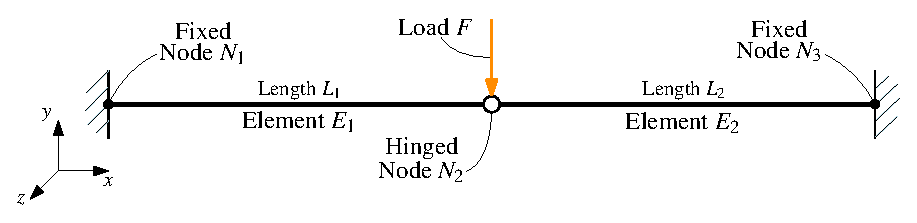
\includegraphics[width=0.8\textwidth]{./figures/appendix_4/usage_example.eps}
  \caption{Simple structure used to demonstrate the usage of the \TrussMe{} package.}
  \label{app4:fig:usage_example}
\end{figure}

To describe the structure in \TrussMe{}, we begin by defining the nodes. The \texttt{MakeNode} function is utilized for this purpose.
%
\begin{verbatim}
> N1 := MakeNode("N1", <0,0,0>, dofs=<0,0,0,0,0,0>):
> N2 := MakeNode("N2", <L_1,0,0>, dofs=<1,1,1,1,1,1>):
> N3 := MakeNode("N3", <L_1+L_2,0,0>, dofs=<0,0,0,0,0,0>):
\end{verbatim}
%
This function requires the node name, coordinates, and \acp{DOF} as inputs. In this case, we have not specified reference frames, so the default ground frame (the identity matrix) is chosen for both nodes. Similarly, no constraints on displacements are specified, so they are assumed to be zero. The \acp{DOF} are set using a six-element vector. The first three elements represent displacements along the $x$-, $y$-, and $z$-axes, while the remaining three represent rotations about these axes. A value of $0$ indicates a constrained \ac{DOF}, while $1$ indicates a free \ac{DOF}. Here, nodes $N_1$ and $N_3$ are constrained in all directions, while $N_2$ is free. The hinge modeling at node $N_2$ will be explained later in this section.

Before defining the elements, the material properties must be specified. Custom materials can be defined using the \texttt{MakeMaterial} function, which requires the material name, Young's modulus, Poisson's ratio, and density as inputs. If the shear modulus is not provided, it is calculated from Young's modulus and Poisson's ratio. In this case, the material is defined as follows.
%
\begin{verbatim}
> M := MakeMaterial(name="GenericMaterial", elastic_modulus=E, shear_modulus=G,
    poisson_ratio=nu, density=rho):
\end{verbatim}
%
Next, the \texttt{MakeBeam} function is employed, necessitating the element's name, nodes at its ends, material, and cross-section properties.
%
\begin{verbatim}
> E1 := MakeBeam("E1", N1, [N2, <0,0,0,0,0,0>], material=M, area=A, inertia=[I_x,I_y,I_z],
    frame=GenerateFrameXY(N1["coordinates"], N2["coordinates"], [0,0,1])):
> E2 := MakeBeam("E2", [N2, <0,0,0,0,0,1>], N3, material=M, area=A, inertia=[I_x,I_y,I_z],
    frame=GenerateFrameXY(N2["coordinates"], N3["coordinates"], [0,0,1])):
\end{verbatim}
%
During the element definition, the reference frame is also specified. Here, the \texttt{GenerateFrameXY} function aligns the coordinate system axes based on the coordinates of the two nodes. Additional details about how the element ends are connected to the nodes can be provided using an augmented six-element vector, such as \texttt{[N, <1,1,1,1,1,1>]}. If this vector is not provided, the element ends are assumed to be rigidly connected to the nodes in all directions. In the provided code snippet, element $E_1$ is connected rigidly to nodes $N_1$ and $N_2$, while element $E_2$ is hinged to node $N_2$ with constrained translational \acp{DOF} and free rotational \acp{DOF}. Element $E_2$ is then rigidly connected to node $N_3$. This hinge connection is achieved by specifying the free rotational \acp{DOF} of the element ends. In this case, element $E_2$ can rotate freely around the $z$-axis.

Once the nodes and elements are defined, the loads acting on the structure can be specified using the \texttt{MakeLoad} function.
%
\begin{verbatim}
> F := MakeLoad("F", N2, <0,-P,0,0,0,0>):
\end{verbatim}
%
Similarly, the \texttt{MakeLoad} function requires the load name, the node where the load is applied, and its magnitude as inputs. Optionally, the load reference frame can be specified using the \texttt{frame} parameter. If not specified, the node's reference frame is used. In this scenario, the load is applied to node $N_2$ in the $y$-direction.

Subsequently, the \ac{FE} model of the structure can be generated using the \texttt{GenerateFEM} function, followed by solving the linear system of equations with \texttt{SolveFEM}.
%
\begin{verbatim}
> fem := GenerateFEM([N1,N2,N3], [E1,E2], [F], tryhard):
> SolveFEM(fem, use_LEM=false, use_LAST=false):
\end{verbatim}
%
When using the \texttt{tryhard} flag, the solvability check described in step (5b) of the list above is activated. To enhance performance, the \TrussMe{} package is designed to complement the \LEM{} and \LAST{} packages, which help manage expression expansion during the symbolic solution procedure. Detailed instructions on utilizing these packages can be found in Section~\ref{chap3:sec:lem} and Section~\ref{chap3:sec:last}, as well as in their respective documentation~\cite{lem, last}. If both libraries are unavailable, the toolbox defaults to utilizing the linear algebra routines built into \Maple{}. If the \LEM{} and \LAST{} packages are preferred for solving the linear system of equations, the \texttt{use\_LEM} and \texttt{use\_LAST} flags must be set to \texttt{true}. In such cases, the solution may be obtained in a veiled form. To unveil the solution, the \texttt{use\_LEM} flag must be set to \texttt{false}. Once the linear system of equations is solved, the solution is stored in the \texttt{fem} table.
%
\begin{verbatim}
> f = fem["f"]^%T; d = fem["d"]^%T;
\end{verbatim}
\begin{equation*}
  \begin{matrix}
    f = \left[\,\begin{matrix}
      \, 0, \, \dfrac{PL_2^3}{L_1^3+L_2^3}, \, 0, \, 0, \, 0, \, \dfrac{PL_1L_2^3}{L_1^3+L_2^3}, \, 0, \, -P, \, 0, \, 0, \, 0, \, 0, \, 0, \, \dfrac{PL_1^3}{L_1^3+L_2^3}, \, 0, \, 0, \, 0, \, -\dfrac{PL_1^3L_2}{L_1^3+L_2^3} \,
    \end{matrix}\,\right] \\[1.5em]
    d = \left[\,\begin{matrix}
      \, 0, \, 0, \, 0, \, 0, \, 0, \, 0, \, 0, \, \dfrac{PL_1^3L_2^3}{3EI_z(L_1^3+L_2^3)}, \, 0, \, 0, \, 0, \, \dfrac{PL_1^2L_2^3}{2EI_z(L_1^3+L_2^3)} \, 0, \, 0, \, 0, \, 0, \, 0, \, 0 \,
    \end{matrix}\,\right]
  \end{matrix}
\end{equation*}

In cases where no symbolic solution could be obtained, or if the user just prefers to assess the solution numerically, the \texttt{GenerateMatlabCode} function can be employed.
%
\begin{verbatim}
> GenerateMatlabCode("FemClass", fem, path="./dir/", info="Usage example class", vars=[P],
    data=[I_x=4.0e-4, I_y=2.0e-4, I_z=2.0e-4, E=210.0e6, nu=0.33, A=5.0e-3, L_1=1.0,
    L_2=1.0]);
\end{verbatim}
%
This function creates the \texttt{FemClass.m} file in the \texttt{./dir/} directory, which contains a class definition of the aforementioned \ac{FE} model. During the code generation process, users can establish default class properties in the \texttt{data} field and variable parameters in the \texttt{vars} field. The latter is intended to represent parameters that may vary during the structure analysis, such as the load magnitude $P$. Further insights into the generated class and its application are elaborated in the subsequent section.

\subsection[The Numerical Computation in \Matlab{}]{The Numerical Computation in Matlab}
\label{app4:subsec:numerical_computation}

Since the symbolic solution of~\eqref{app4:eq:macrodf} may not always be feasible, users have the option to employ a numerical solution. This involves numerically factorizing the $\mathbf{K}^{n}_{ff}$ matrix and evaluating~\eqref{app4:eq:macrosol}. The numerical solution can be achieved within the \Maple{} environment through variable substitution or in \Matlab{} post the code generation process. In the latter scenario, the \TrussMe{} \Matlab{} toolbox comes into play. This toolbox is built upon the \texttt{TrussMe.System} base class, which is utilized to define the components of~\eqref{app4:eq:macrosol} and to establish a unified framework that can be leveraged by inherited classes. Within this abstract class, various methods are present, including several virtual methods that need to be implemented in the inherited classes: \\[0.5em]
%
\begin{minipage}[t]{0.49\textwidth}
  \begin{itemize}
  \setlength{\itemsep}{0.0em}
  \item stiffness matrix $\mathbf{K}^{n}$;
  \item free-free stiffness matrix $\mathbf{K}^{n}_{ff}$;
  \item free-specified stiffness matrix $\mathbf{K}^{n}_{fs}$;
  \item specified-free stiffness matrix $\mathbf{K}^{n}_{sf}$;
  \item specified-specified stiffness matrix $\mathbf{K}^{n}_{ss}$;
  \item displacement vector $\mathbf{d}$*;
  \item free displacement vector $\mathbf{d}^{n}_{f}$*;
  \end{itemize}
\end{minipage}
\hfill
\begin{minipage}[t]{0.49\textwidth}
  \begin{itemize}
  \setlength{\itemsep}{0.0em}
  \item specified displacement vector $\mathbf{d}^{n}_{s}$;
  \item force vector $\mathbf{f}$*;
  \item free force vector $\mathbf{f}^{n}_{f}$;
  \item specified force vector $\mathbf{f}^{n}_{s}$*;
  \item remainder force vector $\mathbf{f}^{n}_{r}$;
  \item \acp{DOF} permutation $\mathbf{P}^{n}$;
  \item getters and setters for the system data;
  \end{itemize}
\end{minipage} \\[0.5em]
%
where (*) denotes that the functionality is accessible only when the symbolic solution of the system is available; otherwise, an empty vector is returned.

\subsubsection{Numerical Computation Usage Example}

The \TrussMe{} \Matlab{} toolbox serves to numerically assess the problem's solution. Utilizing the toolbox is straightforward, particularly when the code is generated using the \TrussMe{} \Maple{} package. Suppose we have generated the \texttt{FemClass.m} file through the \TrussMe{} \Maple{} package; this file encompasses the class definition of the structure. To employ the generated class, we first instantiate it.
%
\begin{verbatim}
>>> fem = FemClass();
\end{verbatim}
%
Optionally, during instantiation, we have the liberty to assign values to the class's internal data.
%
\begin{verbatim}
>>> data.I_x = 4.0e-4; data.I_y = 2.0e-4; data.I_z = 2.0e-4; data.E = 210.0e9; ...
    data.A = 5.0e-3; data.L_1 = 1.0; data.L_2 = 1.0;
>>> fem = FemClass(data);
\end{verbatim}
%
Following instantiation, we can manipulate the internal data values either by setting or retrieving them using dedicated methods.
%
\begin{verbatim}
>>> fem.set_data_field('I_x', 4.0e-4);
>>> I_x = fem.get_data_field('I_x');
>>> fem.set_data(data);
>>> data = fem.get_data();
\end{verbatim}
%
Once instantiated, we can acquire the components of the system of equations~\eqref{app4:eq:macrosol} through the following methods.
%
\begin{verbatim}
>>> x = [1000];
>>> v = fem.v(x);
>>> d = fem.d(x,v);
>>> f = fem.f(x,v);
\end{verbatim}
%
It is worth noting that the vector \texttt{x} includes the system's parameters, such as the load value $P$ of \SSI{1000}{\newton}, while the vector \texttt{v} holds the veiling variables that might have been retained during the symbolic solution computation. In cases where the symbolic solution is unavailable, numerical computation becomes the only viable alternative, which is achieved by invoking the \texttt{compute\_d} and \texttt{compute\_f} methods.
%
\begin{verbatim}
>>> x = [1000];
>>> v = fem.v(x);
>>> d = fem.compute_d(x,v);
>>> f = fem.compute_f(x,v);
\end{verbatim}
%
The least squares solution can also be acquired by incorporating the tolerance value and maximum number of iterations into the \texttt{compute\_d} and \texttt{compute\_f} methods, such as \texttt{fem.compute\_f(x,v,tol,iter)}. Alternative numerical solution methods, relying on constrained minimization of energy functional, can be utilized to solve the system of equations~\eqref{app4:eq:macrosol}~\cite{hutton2004fundamentals}. However, these methods are not currently integrated into the \TrussMe{} \Matlab{} toolbox.

% % % % % % % % % % % % % % % % % % % % % % % % % % % % % % % % % % % % % % % %

\section{Example Applications}
\label{app4:sec:example_applications}

In this section, we briefly showcase two example applications of the \TrussMe{} toolbox. All examples revolve around the rear left double wishbone suspension of the Formula SAE \emph{E-Agle Trento Racing Team} (\emph{University of Trento}) vehicle~\citep{eagle}. The suspension system is depicted in Figure~\ref{app4:fig:suspension}. On the left side, a rendering of the system is shown along with the names of its main components, while on the right side, a schematic representation of the suspension system is presented. In the subsequent paragraphs, we delve into how the \TrussMe{} toolbox can facilitate the design optimization of the suspension system and effectively incorporate the kinematics and compliance of the suspension system through model reduction. The outcomes obtained using the \TrussMe{} toolbox are validated against results obtained from the commercial software \Ansys{}. For a comprehensive analysis of the results from the example applications, please refer to~\cite{larcher2024imece_symbolic}.

\begin{figure}[htb]
  \centering
  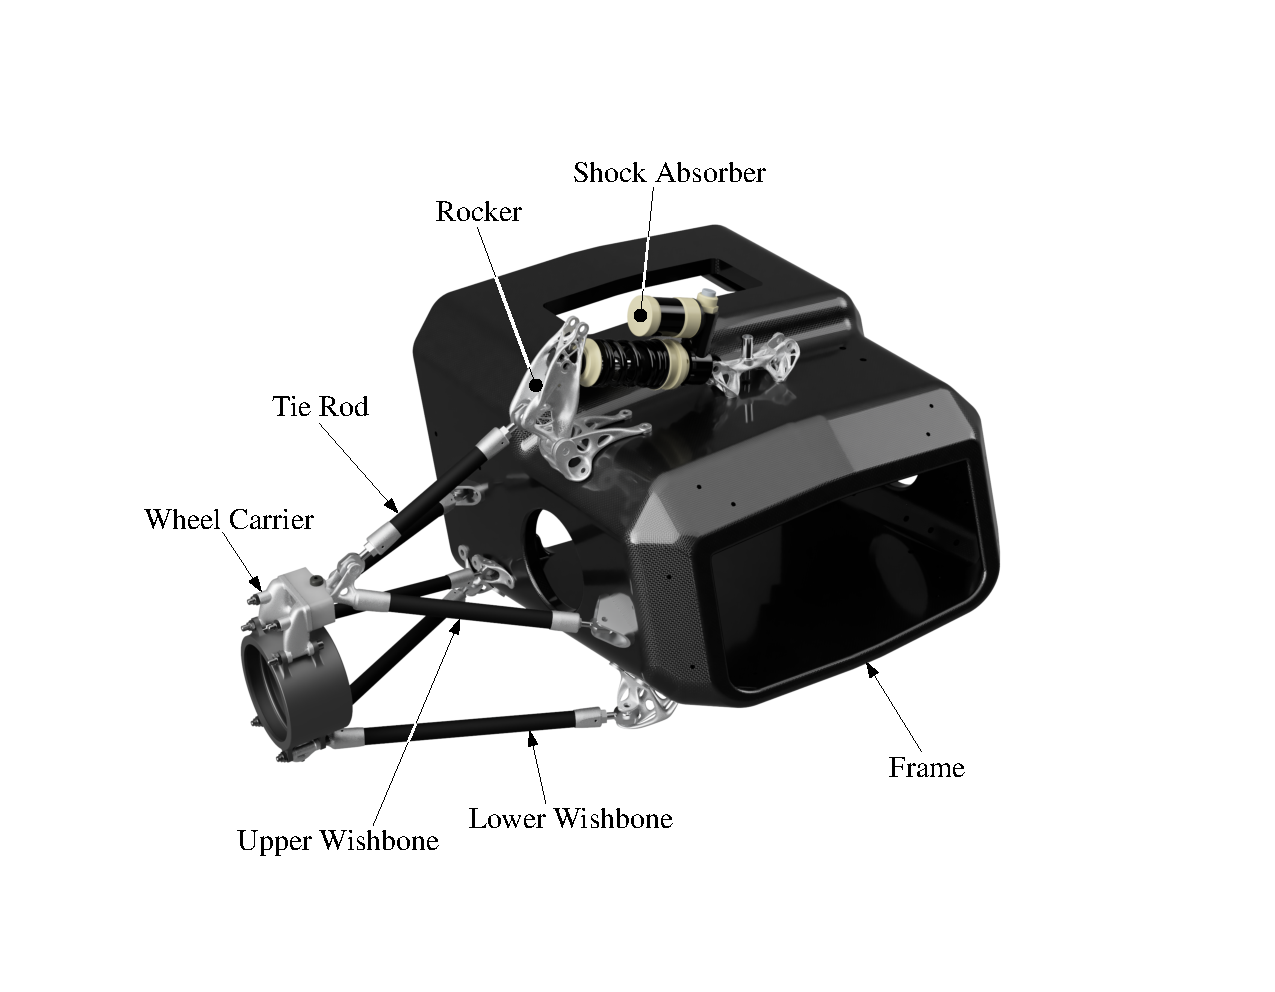
\includegraphics[width=0.475\textwidth, trim={2cm 2cm 3.5cm 2cm}, clip]{./figures/appendix_4/rendering.eps}
  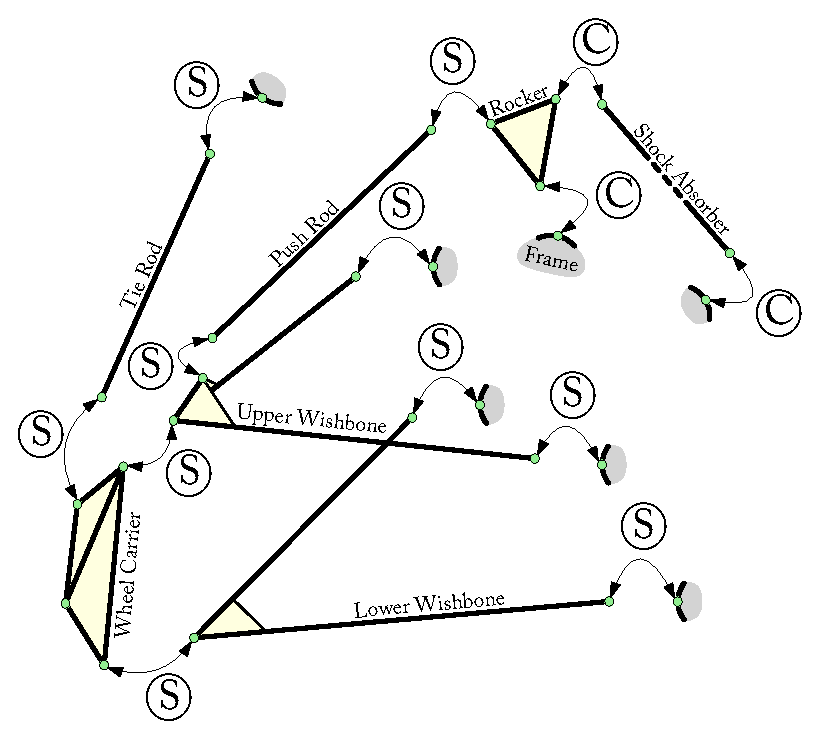
\includegraphics[width=0.425\textwidth]{./figures/appendix_4/constraints.eps}
  \caption{Rendering and schematic representation of the rear left double wishbone suspension. The spherical and cylindrical constraints are respectively represented by the symbols \circled{S} and \circled{C}.}
  \label{app4:fig:suspension}
\end{figure}

Before delving into the example applications, it is essential to clarify the workflow involving the \TrussMe{} package. In this scenario, the \TrussMe{} package is utilized to symbolically assemble the structure and simplify the expressions of its linear system components. Subsequently, the symbolic code is exported into a \Matlab{} class, where internal data and input parameters of the system are specified. This \Matlab{} class is then employed to numerically evaluate the solution of the problem within the \Simulink{} environment. This approach becomes necessary due to the significant slowdown of the symbolic kernel caused by the size and complexity of the resulting linear system.

\subsection{Design Optimization}

Mechanisms involving motion are prevalent in engineering applications. Typically, the design of such mechanisms assumes rigid bodies. However, in certain instances, the flexibility of the mechanism can significantly impact its performance. Optimization emerges as a potent tool for designing structures with optimal performance. The \TrussMe{} toolbox facilitates shape optimization aimed at reducing the compliance of the mechanism and minimizing internal forces. Specifically, the presented optimizations aim to minimize both the wheel compliance hub angle $\theta_z$ and the tie rod axial force $F_a$ by varying the $x$- and $z$- coordinates of the hard point connecting the tie rod to the chassis, referred to as point $P_5$ according to~\cite{larcher2024imece_symbolic}. The results of these optimizations are depicted in Figure~\ref{app4:fig:optimization}. These optimization demonstrations underscore that the current design does not represent the optimal solution in terms of minimum tie rod axial force and minimum wheel compliance hub angle. Optimum conditions are attained through a combination of values indicated by the green point. It is noteworthy that these optimization examples serve solely as a proof of concept for the model's parametric characteristics. In a real-world scenario, a multi-objective optimization considering compliance, structural analysis, and kinematic characteristics of the suspension would be imperative.

\begin{figure}[htb]
  \centering
    \begin{subfigure}[t]{0.49\textwidth}
    \small{\includetikz{figures/appendix_4/optimization_hub_angle.tex}}
    \caption{Wheel hub compliance angle $\theta_z$ dependency from the $x$- and $z$- coordinates of the $P_5$ hard point.}
    \label{app4:fig:variation_theta_z}
  \end{subfigure}
  \hfill
  \begin{subfigure}[t]{0.49\textwidth}
    \centering
    \small{\includetikz{figures/appendix_4/optimization_tie_force.tex}}
    \caption{Tie rod axial force $F_a$ dependency from the $x$- and $z$- coordinates of the $P_5$ hard point.}
    \label{app4:fig:variation_force_tie}
  \end{subfigure}
  \caption{Optimization is conducted on the coordinates of point $P_5$, specifically its $x$- and $z$-coordinates, with the aim of minimizing both the wheel compliance hub angle $\theta_z$ and the tie rod axial force $F_a$. The experiments are conducted under the application of a constant torque $M_z$ of \SI{0.4}{\kilo\newton\meter}. \emph{Marks legend:} {\color{mycolor2}\raisebox{-.15pt}{\Large$\bullet$}} current design, {\color{mycolor5}\raisebox{-.15pt}{\Large$\bullet$}} optimality condition.}
  \label{app4:fig:optimization}
\end{figure}

\subsection{Model Reduction}

This example application explores the inclusion of suspension compliance in vehicle simulation using a hybrid symbolic-numerical approach. This methodology facilitates easy generalization and \ac{RT} modification of model parameters without the need for code regeneration. The suspension's dynamic characteristics are modeled through a system of differential-algebraic equations, integrated using methods described in~\cite{larcher2024imece_symbolic}. Depending on the modeling approach, suspension pick-up points' positions and tire force at the hub are extracted either through semi-analytical solutions or numerical integration. These are then utilized to calculate the suspension's compliance characteristics. The compliance contribution can be incorporated into the overall suspension system displacement as either a \emph{steady-state} or \emph{full dynamic} contribution~\cite{larcher2024imece_symbolic}. The former approach reduces computational costs, while the latter yields accurate simulations at a higher computational expense. Results from this approach are compared with simulation data from commercial software \Ansys{}, showing good agreement under both static (Figure~\ref{app4:fig:rotations} and Figure~\ref{app4:fig:translations}) and dynamic conditions (Figure~\ref{chap5:fig:suspension_dynamic_results} in Chapter~\ref{chap5:applications}).

\begin{figure}[htb]
  \centering
  \small{\includetikz{figures/appendix_4/translations.tex}}
  \caption{Displacements of the wheel carrier reference frame in the $x$-, $y$-, and $z$-axes directions for different loads applied at the wheel hub. In the left-hand side of the figure, the forces are applied and torques are null. Conversely, the right-hand half side of the figure reports the results where torques are applied and forces are null. \emph{Legend:} {\color{mycolor1}$\blacksquare$}~$F_x = \SSI{4.0}{\kilo\newton}$, {\color{mycolor2}$\blacksquare$}~$F_y = \SSI{4.0}{\kilo\newton}$, {\color{mycolor3}$\blacksquare$}~$F_z = \SSI{4.0}{\kilo\newton}$, with $M_x = M_y = M_z = \SSI{0.0}{\kilo\newton\meter}$. {\color{mycolor4}$\blacksquare$}~$M_x = \SSI{0.4}{\kilo\newton\meter}$, {\color{mycolor5}$\blacksquare$}~$M_y = \SSI{0.4}{\kilo\newton\meter}$, {\color{mycolor6}$\blacksquare$}~$M_z = \SSI{0.4}{\kilo\newton\meter}$, with $F_x = F_y = F_z = \SSI{0.0}{\kilo\newton}$.}
  \label{app4:fig:translations}
\end{figure}

\begin{figure}[htb]
  \centering
  \small{\includetikz{figures/appendix_4/rotations.tex}}
  \caption{Rotations of the wheel carrier reference frame around the $x$-, $y$-, and $z$-axes directions for different loads applied at the wheel hub. In the left-hand side of the figure, the forces are applied and torques are null. Conversely, the right-hand half side of the figure reports the results where torques are applied and forces are null. \emph{Legend:} {\color{mycolor1}$\blacksquare$}~$F_x = \SSI{4.0}{\kilo\newton}$, {\color{mycolor2}$\blacksquare$}~$F_y = \SSI{4.0}{\kilo\newton}$, {\color{mycolor3}$\blacksquare$}~$F_z = \SSI{4.0}{\kilo\newton}$, with $M_x = M_y = M_z = \SSI{0.0}{\kilo\newton\meter}$. {\color{mycolor4}$\blacksquare$}~$M_x = \SSI{0.4}{\kilo\newton\meter}$, {\color{mycolor5}$\blacksquare$}~$M_y = \SSI{0.4}{\kilo\newton\meter}$, {\color{mycolor6}$\blacksquare$}~$M_z = \SSI{0.4}{\kilo\newton\meter}$, with $F_x = F_y = F_z = \SSI{0.0}{\kilo\newton}$.}
  \label{app4:fig:rotations}
\end{figure}

% % % % % % % % % % % % % % % % % % % % % % % % % % % % % % % % % % % % % % % %

\end{appendices}

% Bibliography -----------------------------------------------------------------
\addcontentsline{toc}{chapter}{Bibliography}
\DeclareFieldFormat{doi}{%
  \textsc{Doi}\addcolon\space%
  \ifhyperref{%
  \href{https://doi.org/#1}{
    \nolinkurl{#1}
  }
  }{
    \nolinkurl{#1}
  }
}
\printbibliography

% Acknowledgments --------------------------------------------------------------
%\addcontentsline{toc}{chapter}{Acknowledgments (Ringraziamenti)}
%%!TEX root = ../main.tex

\chapter*{Acknowledgments (Ringraziamenti)}
\label{chapter:acknowledgements}

\markboth{ACKNOWLEDGMENTS (RINGRAZIAMENTI)}{}

\subsection*{English version}

I would like to \dots
\bigskip
\hfill{Davide Stocco}

\subsection*{Versione Italiana}

Vorrei ringraziare \dots
\bigskip
\hfill{Davide Stocco}

\vfill


\end{document}

%%%%%%%%%%%%%%%%%%%%%%%%%%%%%%%%%%%%%%%%%%%%%%%%%%%%%%%%%%%%%%%%%%%%%%%%%%%%%%%%
% END DOCUMENT %%%%%%%%%%%%%%%%%%%%%%%%%%%%%%%%%%%%%%%%%%%%%%%%%%%%%%%%%%%%%%%%%
%%%%%%%%%%%%%%%%%%%%%%%%%%%%%%%%%%%%%%%%%%%%%%%%%%%%%%%%%%%%%%%%%%%%%%%%%%%%%%%%
